%Background image credits: https://commons.wikimedia.org/wiki/File:Back_view_of_Venus_reclining_accompanied_by_Cupid_Met_DP887793.jpg Metropolitan Museum of Art, CC0, via Wikimedia Commons
%Background image credits: https://www.flickr.com/photos/9822107@N08/6112497641 Attribution 2.0 Generic shaireproductions.com
%Background image credits: https://commons.wikimedia.org/wiki/File:Dove_(248816)_-_The_Noun_Project.svg I Create Stuff, CC0, via Wikimedia Commons
%Background image credits: https://commons.wikimedia.org/wiki/File:Heraldic_myrtle_wreath.svg Galico, CC BY-SA 3.0, via Wikimedia Commons
%Background image credits: https://commons.wikimedia.org/wiki/File:Venus_geocentric_orbit_curve_simplified_Line_(pentagram).svg AnonMoos, Public domain, via Wikimedia Commons
\documentclass[a4paper, 18pt, oneside]{article}
\usepackage{aurical}
\usepackage[T1]{fontenc}
% Load encoding definitions (after font package)
\usepackage{textalpha}
\usepackage{color}

\usepackage{eso-pic,graphicx}
\usepackage[top=55mm, bottom=55mm, outer=22mm, inner=22mm]{geometry}

\setlength{\columnsep}{120pt}

% Babel package:
\usepackage[main=french,polutonikogreek]{babel}
\usepackage{listings}
\lstset{basicstyle=\ttfamily}

% With XeTeX$\$LuaTeX, load fontspec after babel to use Unicode
% fonts for Latin script and LGR for Greek:
\ifdefined\luatexversion \usepackage{fontspec}\fi
\ifdefined\XeTeXrevision \usepackage{fontspec}\fi

% "Lipsiakos" italic font `cbleipzig`:
\newcommand*{\lishape}{\fontencoding{LGR}\fontfamily{cmr}%
		       \fontshape{li}\selectfont}
\DeclareTextFontCommand{\textli}{\lishape}

\usepackage{booktabs}
\setlength{\emergencystretch}{15pt}
\graphicspath{ {./ } }
\usepackage[figurename=]{caption}
\usepackage{float}
\usepackage{microtype}
\usepackage{setspace}
\onehalfspacing

\makeatletter % change only the display of \thepage, but not \thepage itself:
\patchcmd{\ps@plain}{\thepage}{\Fontlukas\bfseries\color{white}{\thepage}}{}{}
\makeatother

\color{white}

\begin{document}
\pagestyle{plain} % after changing a pagestyle command, it's necessary to invoke it explicitly
\Fontlukas\bfseries
\AddToShipoutPictureBG*{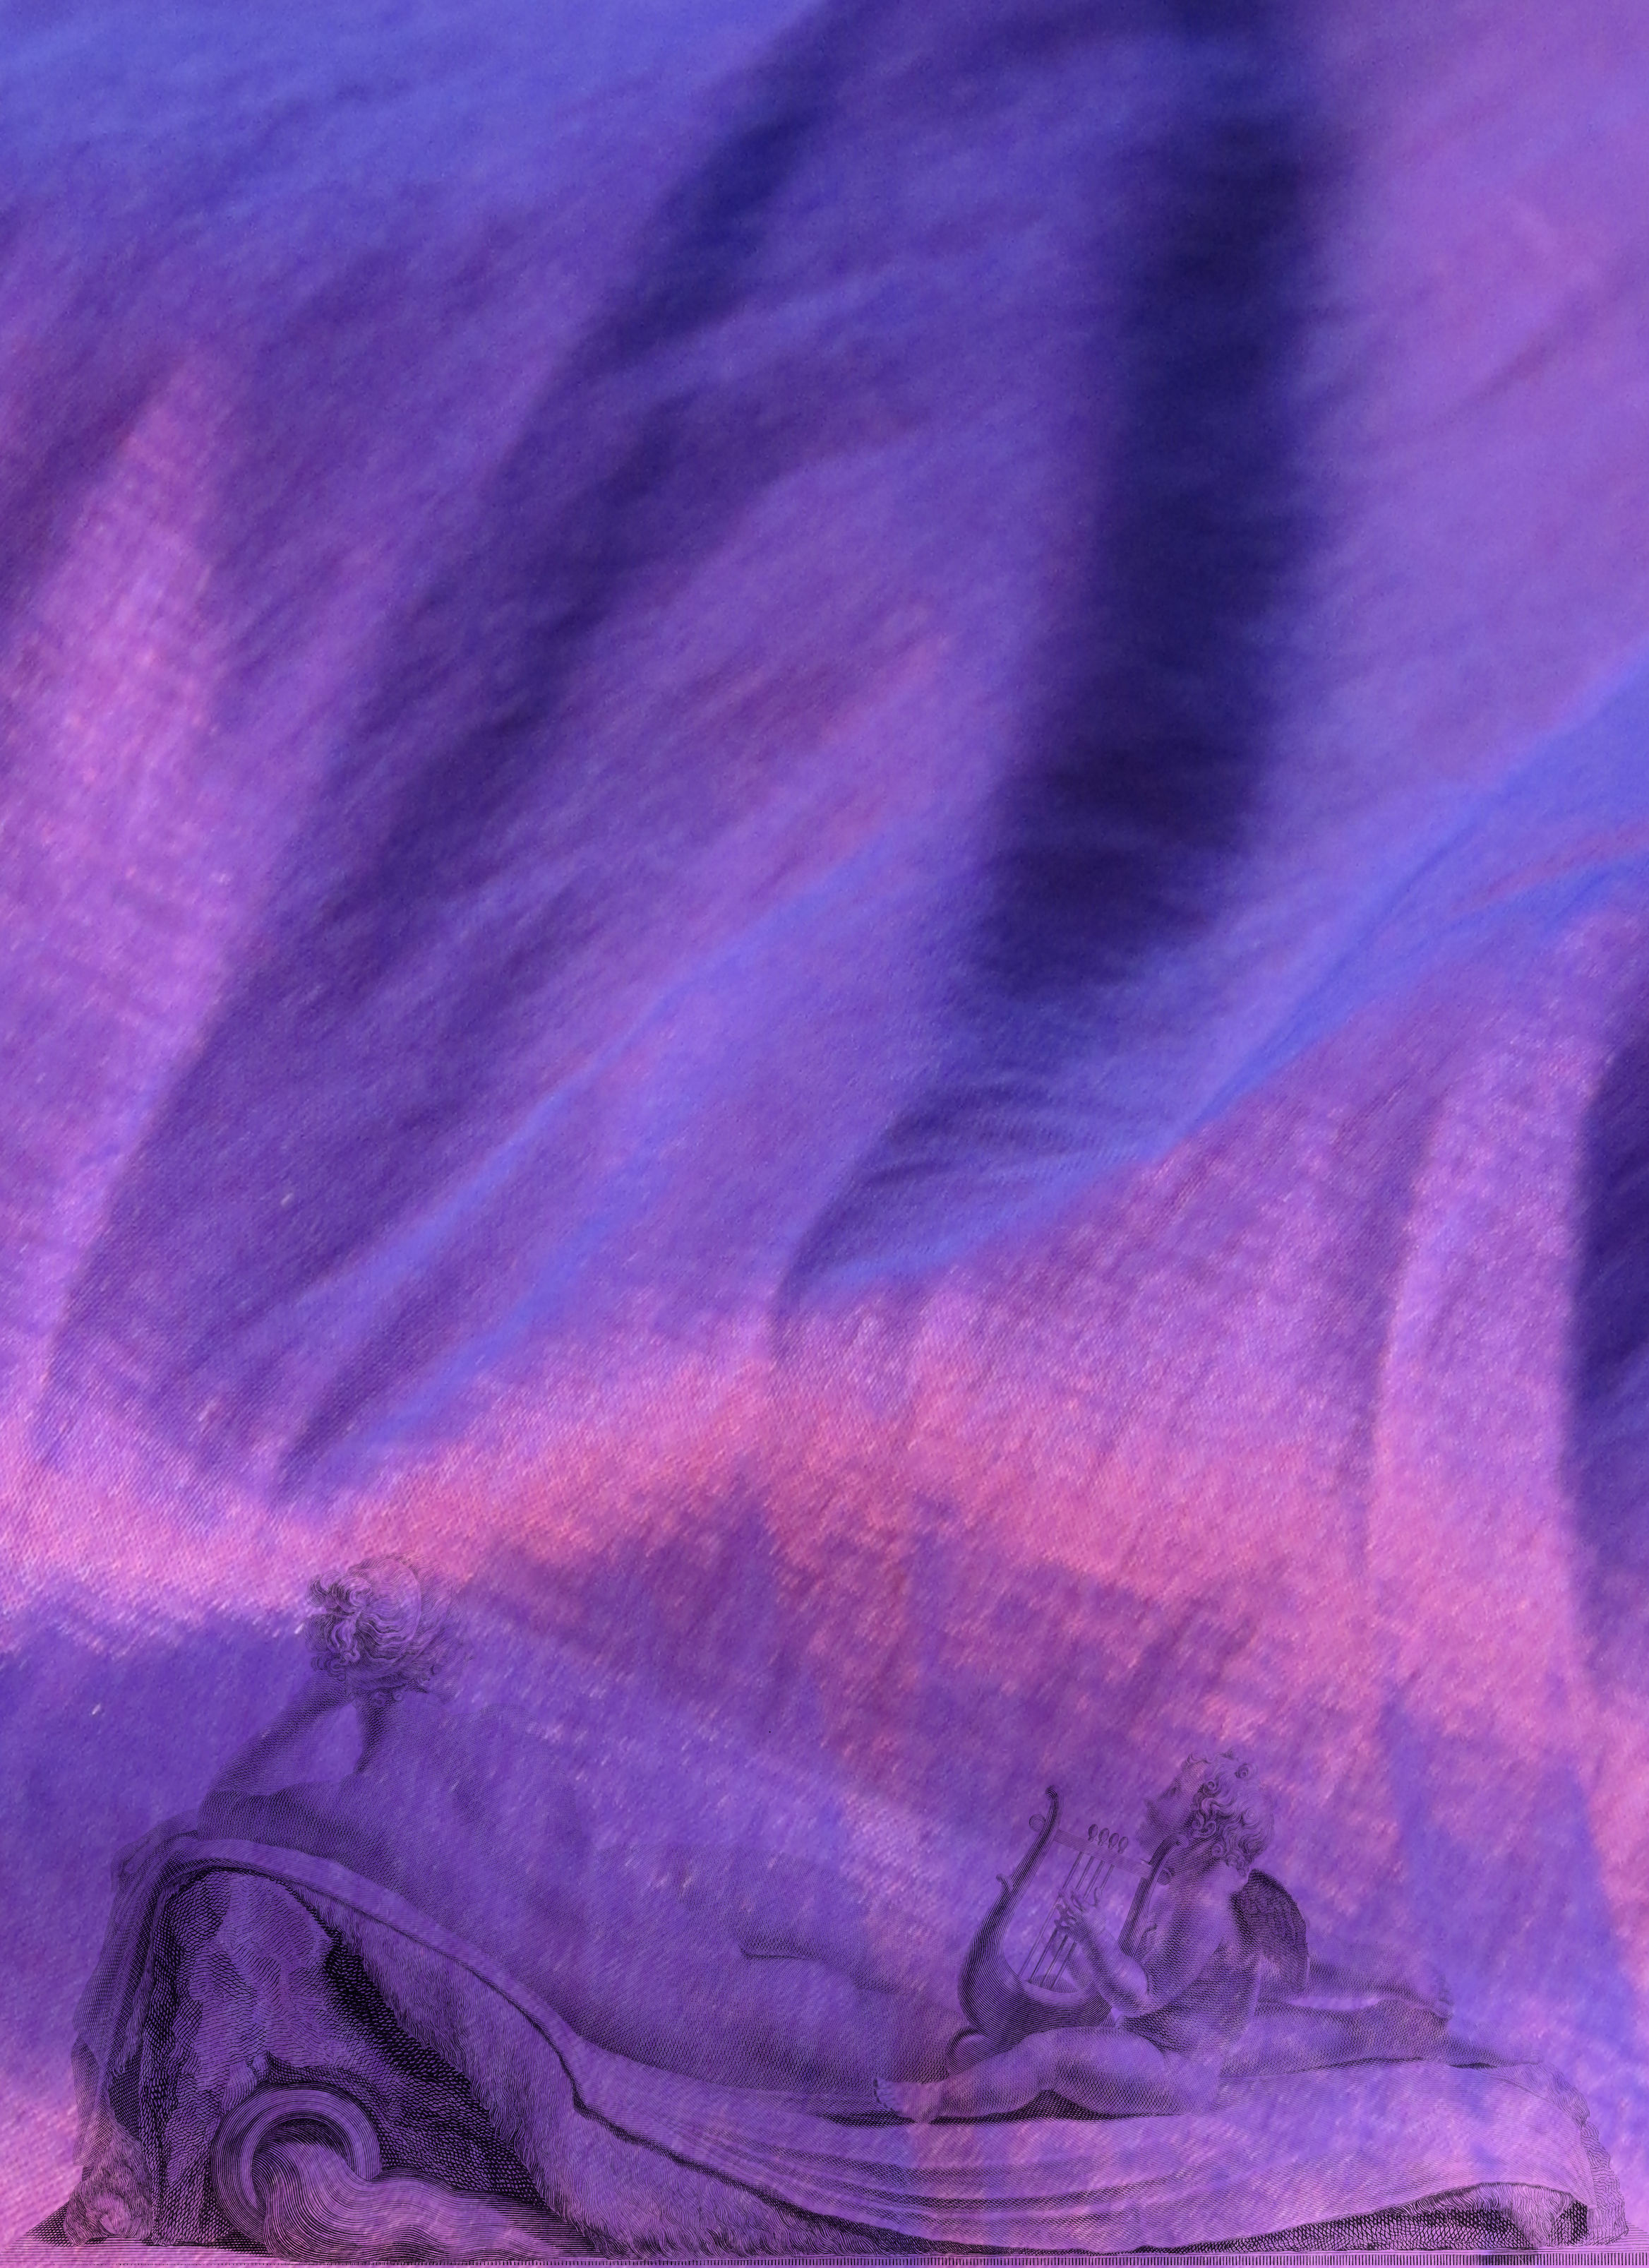
\includegraphics[width=\paperwidth,height=\paperheight]{venus-background-title.jpeg}}

\renewcommand\thefootnote{{\Fontlukas\bfseries\color{white}{\arabic{footnote}}}}
\let\oldfootnote\footnote
    \renewcommand{\footnote}[1]{\oldfootnote{{\normalsize\Fontlukas\bfseries\color{white}#1}}}

\begin{titlepage} % Suppresses headers and footers on the title page
	\centering % Centre everything on the title page
	%\scshape % Use small caps for all text on the title page

	%------------------------------------------------
	%	Title
	%------------------------------------------------
	
	\rule{\textwidth}{1.6pt}\vspace*{-\baselineskip}\vspace*{2pt} % Thick horizontal rule
	\rule{\textwidth}{0.4pt} % Thin horizontal rule
	
	\vspace{1\baselineskip} % Whitespace above the title
	
	{\scshape\Huge Mémoire sur la Déesse Vénus,}
	
	\vspace{1\baselineskip} % Whitespace above the title

	\rule{\textwidth}{0.4pt}\vspace*{-\baselineskip}\vspace{3.2pt} % Thin horizontal rule
	\rule{\textwidth}{1.6pt} % Thick horizontal rule
	
	\vspace{1\baselineskip} % Whitespace after the title block
	
	%------------------------------------------------
	%	Subtitle
	%------------------------------------------------

 {\scshape Auquel l'Académie Royale des Inscriptions et Belles-Lettres\\ a adjugé le Prix de la Saint Martin 1775.} % Subtitle or further description

 	\vspace*{1\baselineskip} % Whitespace under the subtitle

	{\scshape \Large Par Pierre-Henri Larcher,} % Subtitle or further description

 	\vspace*{1\baselineskip} % Whitespace under the subtitle

{\scshape De l'Académie des Sciences et Belles-Lettres de Dijon.} % Subtitle or further description

	%------------------------------------------------
	%	Editor(s)
	%------------------------------------------------
\vspace*{\fill}

	\vspace{1\baselineskip}

	{\small\scshape A Paris, 1776.}
	
	{\small\scshape{Chez Valade, Libraire, rue S. Jacques,\\ vis-à-vis la rue des Mathurins.}}
	
	\vspace{0.5\baselineskip} % Whitespace after the title block

\scshape Internet Archive Online Edition% Publication year
	
	{\scshape\small Utilisation non commerciale --- Partage dans les mêmes conditions 4.0 International} % Publisher
\end{titlepage}
\setlength{\parskip}{1mm plus1mm minus1mm}
\clearpage
\Large

\AddToShipoutPictureBG{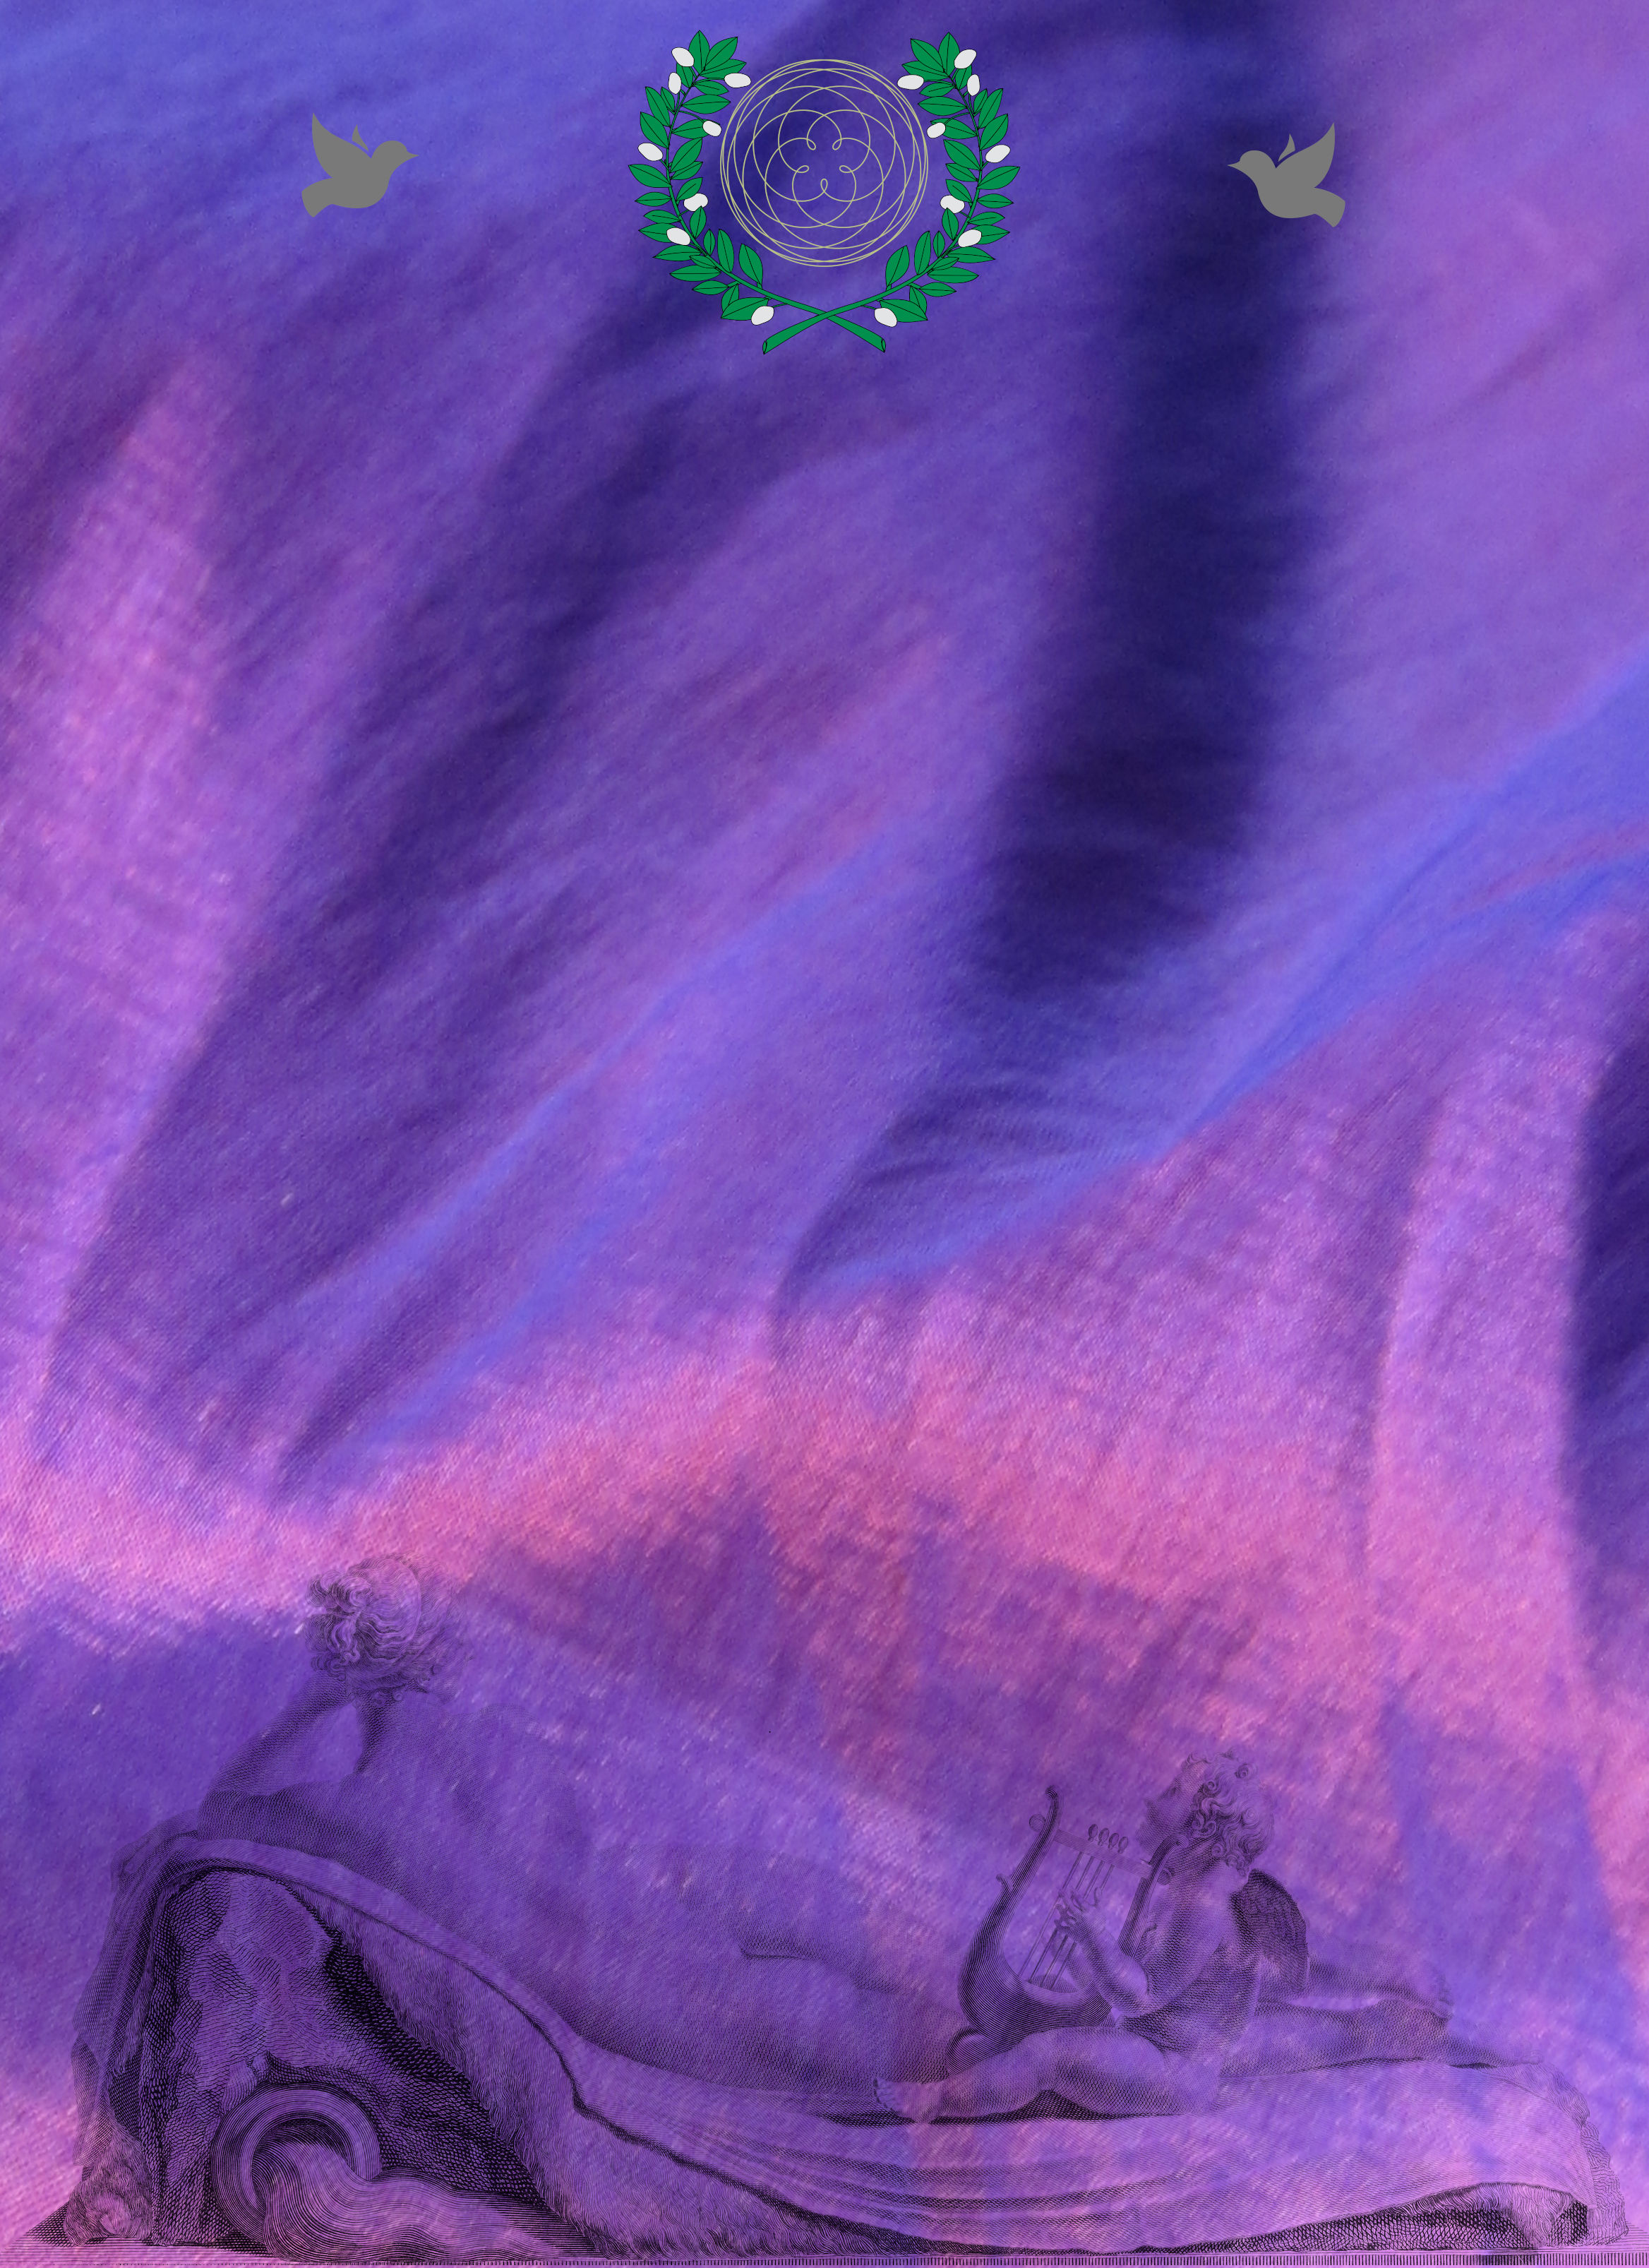
\includegraphics[width=\paperwidth,height=\paperheight]{venus-background.jpeg}}
\paragraph{}
\emph{L'Académie a proposé pour sujet du Prix, quels furent les Noms et les Attributs divers de Vénus chez les différents Peuples de la Grèce et de l'Italie ; quelles furent l'origine et les raisons de ces Attributs ; quel a été son Culte ; quels ont été les Statues, les Temples, les Tableaux célèbres de cette Divinité, et les Artistes qui se sont illustrés par ces Ouvrages.}

Ce sujet flatte agréablement l'imagination. Les fleurs semblent éclore sous les pas de la Déesse, et une mythologie enchanteresse offre mille tableaux riants, à la faveur d'un choix heureux, en proscrivant avec soin l'érudition, et en ne présentant que des surfaces légères, on ferait sans doute un morceau piquant, agréable et pittoresque, \emph{quæ legat ipsa Lycoris} ; mais on n'aurait pas rempli les vues de l'Académie. Si on ne rassemble pas en effet tous les traits épars dans une multitude d'Auteurs, cet ouvrage sera tronqué, imparfait, et sans les autorités sur lesquelles ces faits sont appuyés, il sera dénué du genre de preuves qui en est la base, et qui lui donne toute sa consistance. Cette méthode indispensable répand nécessairement de la sécheresse sur un sujet qui ne promettait que des grâces, et cette sécheresse doit augmenter par la nomenclature, souvent stérile, mais toujours nécessaire, des noms, surnoms et épithètes de cette Déesse, et par celle de tous les Temples, Autels et Statues qu'on lui a élevés. Mais à travers ces landes et ces terres arides, il se trouve des fleurs à cueillir: toutes les fois que mon sujet me les offrira de lui-même, je croirai bien mériter de mes Juges, en mêlant pour eux l'agréable à l'utile.

Qu'on ne s'imagine pas suffire au plan de l'Académie à l'aide des Tables des Matières qui sont à la fin des Auteurs, et sans la connaissance de la Langue Grecque. La plupart de ces Tables sont très-imparfaites, comme je l'ai éprouvé. La seule lecture de Pausanias m'a fourni plus de trente, tant noms, que Temples et Autels de Vénus omis dans l'Index de cet Auteur. A l'égard de l'intelligence de la Langue Grecque, elle est indispensable ; puisque sans elle on court risque à tout instant de tomber dans des contresens innombrables des Traducteurs Latins et François. Ce n'est point même assez de posséder passablement cette Langue, il faut encore la savoir en Critique ; car on rencontre sur sa route beaucoup de passages altérés, et sans ce degré de connaissance, on s'expose à faire dire à un Auteur le contraire de ce qu'il a voulu dire, et l'on donne contre des écueils fameux par plus d'un naufrage. J'ai souvent été obligé, par cette raison, de restituer des textes altérés, et j'ai cru suivre en cela les vues de l'Académie, qui sait que l'intelligence des faits dépend de celle des Auteurs.

Si nous avions l'Ouvrage de\footnote{Diogen. Laert. lib. 2. segment. 47. pag. 109. Voyez aussi la Note de Ménage. Le Scholiaste d'Apollonius Rhodius (ex edit. Aldi, pag. 135. lin. 6.) cite ce Socrate de Cos, ἐν ταῖς ἐπικλήσταιστι ; mais il faut lire ἐπικλήστεστι dans les Dénominations. L'αι se confond souvent avec dans l'ε dans les manuscrits.} Socrate de Cos sur les surnoms des Dieux, et les événements qui y avoient donné occasion, le plan de l'Académie serait en partie rempli, et content d'y renvoyer, je passerais aux Temples et aux Statues élevés en l'honneur de Vénus. Mais, puisque ce Livre n'est point venu jusqu'à nous, je vais tâcher d'en réparer la perte le mieux que je pourrai, en rassemblant en un seul et même corps tout ce que les Anciens nous ont laissé sur cette Déesse.

C'est avec raison que Théocrite félicite Vénus sur la multitude de noms qu'on lui a donnés et de Temples qu'on lui a élevés, πολυώνυμε καὶ πολύναε.\footnote{Theocrit. Idyll. 15. vers. 109.} Jamais Déesse a-t-elle en effet été connue sous un plus grand nombre de rapports, ou a-t-elle eu un culte plus étendu ?

Née dans l'Orient, elle y fut connue sous les noms de Mylitta, de Mitra, d'Alitta, \emph{etc.} Elle passa delà chez les Peuples Occidentaux, qui l'appelèrent Uranie, et fut adorée sous ce nom en différents lieux de la Grèce, et particulièrement à Athènes. L'ordre exige donc que je commence par la Vénus des Asiatiques ; mais comme l'Académie borne les recherches sur les noms et les attributs de cette Déesse aux différents Peuples de la Grèce et de l'Italie, je le ferai d'une manière succincte, et je me contenterai de rapporter les faits, sans bâtir de systèmes, ce qui serait très-aisé, et sans analyser ceux des autres, ce qui le serait encore davantage. Rien ne serait en effet plus facile que de compiler les ouvrages des Bochart, des Selden, \emph{etc.} et de surcharger cette Dissertation d'une érudition Orientale, qui n'en imposerait qu'à ceux qui n'y seraient pas initiés. Mais ce serait abuser de la patience de l'Académie, et lui enlever un tems précieux aux Lettres, et dont elle sait faire un si bon emploi. Ajoutons que les Ecrits des Orientaux ne sont pas venus jusqu'à nous. Les Grecs et les Latins, auxquels je suis obligé de recourir, en disent peu de chose, et je me flatte que l'Académie, qui connait mieux que personne le peu de secours qu'on peut tirer de leurs Ouvrages, voudra bien excuser si cette partie de mon Mémoire ne répond pas à l'idée que pourraient s'en former des personnes qui sentent le prix des connaissances, et ignorent la modicité des ressources.

Je n'examinerai point si l'Asie, qui est le berceau de la vraie Religion, n'est pas aussi celui de toutes les superstitions; il suffit seulement de savoir que si elles n'y sont pas nées, elles y trouvèrent un sol fertile, une terre préparée à les recevoir et à les propager.

Les Grecs empruntèrent leur Vénus des Orientaux. Mais quelle fut son origine chez ceux-ci ? Ils avoient plusieurs systèmes de Philosophie. Les uns vouaient que l'air fut le principe de tout ; d'autres prétendaient que ce fut l'eau ; d'autres enfin que ce fut le feu. Ces Peuples d'une imagination vive, et accoutumés à tout allégoriser, représentaient, sous l'emblème de Vénus, la force vivifiante de la Nature, la Cause Universelle. Delà, elle est tantôt l'air, tantôt elle naît de la mer, et tantôt c'est une semence ignée qui tombe du ciel dans les eaux. Selon le premier de ces systèmes : « Les Assyriens, dit\footnote{Julius Firmicus Maternus de Errore Profanarum Religionum. pag. 9.} Julius Firmicus Maternus, et une partie des Africains, non content de regarder l'air comme le premier des éléments, l'adoraient et le représentaient d'une manière figurée. Ils le nommaient alors Junon ou Vénus Vierge. »

Ce qui n'était d'abord qu'un emblème, qu'un type devint un être réel. Cette force vivifiante fut appelée chez les Assyriens Mylitta, ou plutôt Mylidath, qui signifie Genetrix en Chaldéen, selon\footnote{Selden de Dîs Syris. Syntagm. 2. cap. 2. pag. 174 et 175.} Scaliger. Le Mitra des Perses et l'Alitta ou Alilat des Arabes, dont parle\footnote{Hérodot. lib. 1. §. 131. lib. 3. §. 8.} Hérodote, ont aussi la même signification, si l'on en croit\footnote{Selden de Dîs Syris. Syntagm. 2. cap. 2. pag. 179 et 180.} Selden.

Ceux qui regardaient le feu comme le principe générateur, la faisaient fille de Cœlus ou Uranus. Un\footnote{Joan. Antiocheni Malalæ Historia Chronica, lib. 2. pag. 19. comme les deux premiers livres de Malalas ne sont point venus jusqu'à nous, l'Editeur y a suppléé par les Extraits de Chronologie d'un Anonyme. C'est dans ces Extraits que se trouve le passage que je cite.} Anonyme, dont les Extraits de Chronologie sont à la tête de Malalas, prétendait qu'elle était femme de Cœlus, et lui donnait Saturne pour fils. Mais je m'arrête d'autant moins à cette opinion, que cet Auteur, quel qu'il soit, paraît très-ignorant.

Ceux qui croyaient l'eau le premier principe, le premier agent, la firent naître dans la mer. Je développerai cela en un autre endroit. Elle était fille de Cœlus et de Dies, suivant\footnote{Cicero de Naturâ Deorum, lib. 3. §. 23. Arnobe adversus gentes (lib. 4. pag. 136.) en compte à tant, mais sans les spécifier.} Cicéron, et c'est la première des quatre Vénus qu'il compte d'après les Anciens. Platon\footnote{Plato Symposiæ. tom. 3. pag. 180. D.} ne lui donnait point de mère. La seconde, selon le même.\footnote{Cicero loco superius laudato.} Cicéron, engendrée de l'écume de la mer, eut de Mercure le second Cupidon ; la troisième, fille de Jupiter et de Dioné, épousa Vulcain, mais elle eut de Mars Antéros. La quatrième est la Syrienne, conçue à Tyr. Elle se nomme Astarté, et on lui donne Adonis pour époux.

Ces quatre Vénus tiennent à l'un ou à l'autre de ces systèmes, et sont conséquemment au fonds les mêmes. Aussi la plupart des Ecrivains Anciens les ont-ils confondues. J'espère qu'on ne me saura pas mauvais gré de l'avoir fait à leur exemple. J'observerai cependant dans ce Mémoire le plus d'ordre qu'il me sera possible.

La Vénus, que Cicéron nomme la première, comme je viens de le remarquer, était fille de Cœlus et de Dies ; mais, suivant\footnote{Plato Sympos. tom. 3. pag. 180. D.} Platon, elle reconnaissait le même père, et n'avait point de mère. Plus connue sous le nom de Vénus Uranie ou Céleste, elle unit dès l'origine\footnote{Apul. Metamorphos. lib. 11. pag. 357 et 358.} du monde les deux sexes, et perpétua ainsi la race humaine. \emph{Cœlestis Venus quæ primis rerum exordiis sexuum diversitatem generato amore sociasti, et æternâ sobole humano genere propagato, nunc... coleris, etc.} Cet attribut, qui lui est commun avec la mère de l'Amour, ou la fille de Dioné, fait voir que les Grecs et les Latins avoient emprunté leur Vénus des Orientaux, et qu'ils avoient embelli, ou pour mieux dire, dénaturé les fables de ces Peuples, comme tout ce qui passait par leurs mains.

Elle était la Cause Universelle répandue dans toute la nature, πάντα γὰρ ἐκ στέθεν ἐσττὶν.\footnote{Orphei Hymn. 54. vers. 4.} C'est sous ce point de vue qu'Orphée a dit, que tout ce qui respirait dans le ciel, sur la terre, et dans les abîmes de la mer, était son ouvrage.
\begin{quotation} 
\hspace*{15mm}Γεννᾷς δὲ τά πάντα

ὅστστάτ᾽ ἐν οὐρανῷ ἐσττι καὶ ἐν γαίη πολυκάρπῳ,

Ἐν πόντῳ τε βυθῷ τε.\footnote{Orphei Hymn. 54. vers. 5.}
\end{quotation}
\paragraph{}
Ces Vers prouvent que le sentiment de Barthius, qui faisait dire à Lucrece\footnote{Dans ces vers de l'Invocation : Æneadum genetrix, hominum Divûmque voluptas, Alma Venus, cœli sueter-labentia signa, Quæ mare navigerum, quæ terras singiferentes Concelebras...} que Vénus avoir peuplé le Ciel, en faisant de \emph{subter labentia} un seul mot, régime de \emph{concelebras}, n'était pas aussi absurde que le pensait Creech, le meilleur Commentateur de ce Poète Philosophe. Il ignorait sans doute que, selon l'ancienne mythologie, Vénus Uranie était la mère des Dieux. Servius, au défaut d'Orphée, aurait pu le lui apprendre : \emph{Dicunt\footnote{Servius ad Virgilii Æneid. lib. 10. vers. 83.} ipsam Venerem esse matrem Deûm}.

Cette Déesse exerçait un empire souverain sur les Parques,\footnote{Orph. Hymn. 54. vers. 5.} Κρατέεις τριστστεεῶν Μοιρῶν. Aussi Proclus de Lycie assure-t-il, dans un Hymne, qu'il lui\footnote{Procli Hymn. 1. in Venerem. vers. 7. etc.} adresse, que les Grands de Lycie avoient souvent évité les traits de la mort par sa puissance.

Elle était Vierge\footnote{Id. ibid. vers. 1.} Κουραφροδίτη. Julius Firmicus Maternus\footnote{Julius Firmicus Maternus de Errore Profanarum Religionum, pag. 9.} parle aussi de Vénus Vierge, ce qui ne peut convenir qu'à Vénus Uranie ; mais comme cet Auteur ne paraît point en avoir eu connaissance, il ajoute tout de suite : \emph{Si tamen Veneriplacuit aliquando Virginitas}.

Elle présidait aux chastes amours ; de-là vient que le même Proclus finit son premier Hymne à Vénus, par la prier d'éloigner de lui ce qui peut le couvrir de honte, de l'élever à l'amour de l'honnête, et de réprimer les désirs effrénés d'un amour terrestre. De là vient aussi qu'Orphée\footnote{Orphei Hymn. 54. vers. 28.} la prie de recevoir favorablement les vœux qu'il lui adresse avec un cœur pur. Le second Hymne de Proclus, en son honneur, roule entièrement sur le même sujet ; mais je le laisse de côté, afin de ne point trop allonger ce Mémoire.

Les Assyriens\footnote{Pausanias Attic. sivè, lib. 1. cap. 14. pag. 36.} l'honorèrent avant tous les autres Peuples. C'est d'eux que les habitants de Paphos reçurent son culte, qu'ils communiquèrent aux Phéniciens qui habitaient Ascalon en Palestine, et les Phéniciens le transmirent à ceux de Cytheres.

Hérodote\footnote{Herodot. lib. 1. §. 105.} dit la même chose, à cela près qu'il assure que le Temple d'Ascalon était le plus ancien ; que celui de Cypre en tirait son origine ; et que celui de Cytheres avait été bâti par des Phéniciens de la Palestine. Cet Historien ne parle point en ce passage des Assyriens ; mais il avance\footnote{Id. ibid. §. 131.} plus bas que les Perses tenaient le culte de Vénus Céleste des Assyriens et des Arabes ; que les Assyriens donnaient à Vénus le nom de Mylitta, les Arabes celui d'Alitta, et les Perses celui de Mitra. Cela est confirmé en partie par Saint Ambroise contre Symmaque\footnote{Stus Ambrosius adversus Symmachum. lib. 2. pag. 840.} : \emph{Cœlestem Afri, Mitram Persæ, plerique Venerem colunt, pro diversi ate nominis, non pro numinis varietate}.

On voit par-là que la Déesse Mylitta, adorée à Babylone, était la même qu'Uranie. Hésychius dit aussi la même chose au mot Μύλητα. Son culte était pur dans l'origine ; mais bientôt il dégénéra, et les endroits, où l'on s'assemblait pour lui rendre hommage, devinrent, dans la suite, des lieux de prostitution. C'est un fait avéré, et reconnu par tous les Ecrivains de l'antiquité. S'opposer à leur témoignage, c'est établir dans l'Histoire ancienne un Pyrrhonisme capable de refluer sur l'Histoire moderne, et de lui porter des coups très-dangereux.

Les femmes se prostituaient à Babylone, une fois en leur vie, en l'honneur de cette Déesse. Elles attendaient\footnote{Herodot. lib. 1. §. 199.} dans son Temple l'arrivée des étrangers. Lorsqu'une femme y avait pris place, elle ne pouvait s'en retourner chez elle, qu'un étranger ne lui eut jette de l'argent sur les genoux, en lui disant : J'invoque la Déesse Mylitta, et qu'il n'eût eu commerce avec elle hors du lieu sacré. Le Prophète Jérémie\footnote{Baruch cap. 6. \emph{vir}. 42 et 43.} parle clairement de cet usage, dans la Lettre qu'il écrit aux Juifs, qui dévoient être emmenés captifs à Babylone.

Il y avait des coutumes à peu près semblables en quelques endroits de l'Isle de Cypre, comme le dit Hérodote au même paragraphe, à\footnote{Euseb Vit. Constantin. lib. 3. cap. 58. pag. 613. Socrat. Hist. Ecclesiastic. lib. 1. cap. 18. tom. 2. pag. 48.} Héliopolis en Phénicie, et à Aphaques, près du Liban. Constantin abolit cet usage infame dans ces deux Villes et détruisit leurs Temples.

Zosime, qui s'étend sur le culte de Vénus à Aphaques, ne parle point de cette prostitution ; il se contente\footnote{Zosim. Histor. lib. 1. pag. 53.} de faire remarquer que les jours de fête de la Déesse, on apercevait en l'air, aux environs du Temple, un globe de feu, ou une torche allumée, et que les dons qu'on offrait à la Déesse se mettaient sur les eaux du lac près de ce Temple, et que s'ils lui étaient agréables, ils allaient au fonds, et qu'autrement ils surnageaient.

Ce fut en cette ville que Vénus donna à Adonis le premier et le dernier embrassement, suivant l'Auteur de l'Etymologicum Magnum, qui nous apprend au mot Αφακα, qu'Aphaca signifie en Syriaque\footnote{M. de Villoison, qui possède aussi-bien les Langues Orientales que le Grec, m'a communiqué cette note, ci-après que le Prix m'a été adjugé.\\\hspace*{5mm}« L'Auteur de l'Etymologicum magnum a bien raison d'observer que ce nom d'une Ville, située près du Liban, est Syriaque, et qu'il signifie \emph{s'embrasser}. On retrouve encore le mot d'Aphak en ce sens, dans la version Syriaque des Actes des Apôtres, chap. 20. vers. 10. dans la version Syriaque de la Genèse, chapitre 29. \emph{vir}. 13 et chap. 33. \emph{vir}. 4. et dans celle du quatrième Livre des Rois, chap. 4. \emph{vir}. 16. Il est singulier que ce mot, propre et particulier au Syriaque, ne se retrouve ni dans le Chaldéen, ni dans l'Hébreu, ni dans l'Arabe, ni dans l'Ethiopien, langues qui ont le même fond, les mêmes racines et la même marche que le Syriaque, et qui ne sont toutes que des dialectes de la Langue Orientale ; rapports si évidens, que Strabon en a été frappé, lorsqu'il observe (lib. 1. pag. 70. ed. d'Amsterd.) que les Arméniens, les Syriens et les Arabes se ressemblent beaucoup dans leurs langues, leur manière de vivre et la forme de leurs corps, » τὸ γὰρ τῶν Αρμενίων ἔθνος καὶ τὸ τῶν Σύρων, καὶ τῶν Αράβων, πολλὴν ὀμοφυλίαν ἐμφαίνει, κατά τε τὴν διάλεκτον, καὶ τοὺς βίους, καὶ τους τῶν στωμάτων χαρακτήρας καὶ μάλισττα καθὸ πληστιόχωροι ἐιστὶ.} un baiser. Cette Vénus avait aussi nom\footnote{Macrob. Saturnal. lib. 1. cap. 21. pag. 209.} Architis, probablement d'Arca, ville dans le voisinage d'Aphaques, où elle était adorée. Ainsi, je ne vois pas la nécessité de changer avec Pontanus cette dénomination.

Valère Maxime nous apprend\footnote{Valer. maxim. lib. 2. cap. 6. §. 15. pag. 181.} qu'on observait à Sicca Veneria en Afrique un usage pareil à celui de Babylone. Cette ville était éloignée d'environ cent vingt milles de Carthage. C'était une Colonie Phénicienne. Or il est très-vraisemblable que ses habitants avoient reçu le culte de cette Vénus des Phéniciens.

Le Temple de Vénus Céleste à Ascalon\footnote{Herodot. lib. 1. §. 105 et 106.} fut pillé par des Soldats de l'arrière garde de cette Armée Scythe, qui asservit l'Asie pendant vingt-huit ans, et qui, voulant pousser ses conquêtes en Egypte, en fut détournée par les présents que lui fit Psammitichus. La Déesse se vengea sur les Scythes qui avoient pillé son Temple, par une maladie honteuse dont elle les affligea. Je n'entrerai point dans une explication de cette maladie ; cela m'éloignerait trop de mon sujet.

Les Babyloniens nommaient aussi Vénus Molis. « Il jura\footnote{Damascenus in excerptis Valesianis, pag. 439.} par Molis : car tel est le nom que les Babyloniens donnent à Vénus. » Serait-ce une faute des copistes pour Mylitta ? je n'oserais le décider.

Les Babyloniens l'appelaient encore Salambo, selon Hésychius ; mais ils ne peuvent point s'être servis de ce terme, qui est grec, et qui tire son origine de στάλα, qui signifie au propre l'agitation de la mer, et au figuré celle de l'âme. De στάλα viennent σαλαΐζειν\footnote{Hésychius Σάλα, φροντίς. Σαλαίζειν, κόπτεστθαι. Σαλαΐς, κωκυτός. Σαλάβη, φραντίς.} se frapper le sein, comme dans le deuil, déplorer une perte. Σαλαΐς des gémissements. Σαλάβη l'agitation de l'âme. « Σαλαμβάς une Déesse ainsi nommée, dit l'Auteur de l'Etymologicum magnum, parce qu'elle va de côté et d'autre pleurant Adonis. Anacréon employé, continue le même Auteur, le mot σαλαΐζειν pour pleurer, déplorer, car une douleur et des gémissements pareils agitent l'âme et la troublent. » Ainsi, Salambo signifie Vénus pleurant la mort d'Adonis.

Déléphat était pareillement un nom de Vénus, selon\footnote{Selden de Dîs Syris. Syntagm, 2. 100. 4. p. 210.} Selden ; mais Héyschius, de l'autorité de qui il s'appuyé, dit seulement que c'est ainsi que les Chaldéens nommaient l'astre de Vénus.

La Déesse de Syrie passait aussi pour une Vénus ; et il est d'autant plus vraisemblable que c'en était une, qu'on la\footnote{Plutarch. in Crasso, pag. 553. F.} regardait comme la Nature et la première Cause qui de l'humidité tire les principes et les semences de toutes choses, et qui a découvert la source de tous les biens qui arrivent aux hommes. Hygin assure pareillement que\footnote{Hygini Fabulæ 198. Vide Auctores Mythographos Latinos, pag. 327.} cette Déesse était Vénus. Il tomba du ciel dans l'Euphrate, dit-il, un œuf d'une grandeur merveilleuse. Les poissons l'ayant roulé sur le rivage, des colombes le couvèrent, et l'ayant fait éclore, Vénus en sortit. Jupiter mit les poissons au nombre des astres, à la prière de la Déesse, dont il voulait récompenser la justice et la probité. Les Syriens, ajoute Hygin, regardent par cette raison les poissons et les colombes comme des dieux, et n'en mangent jamais.

Cette Déesse s'appelait Atargatis, suivant Strabon\footnote{Strabo, lib 16. pag. 1085. A.} ; mais si l'on en croit Eratosthène dans ses Κατασττεριστμοί,\footnote{Erathostenis enarrationes eorum quæ in astra sunt relata, pag. 13.} elle se nommait Dercéto. Elle tomba, dit-il, pendant la nuit, dans un lac près de Bambyce, (c'est la ville d'Héliopolis, selon Appien de Bello Parthico,\footnote{Appianus, pag. 270. Conf. Strab. lib. 16. 1084, lin. ultimâ et Plin. lib. 5. cap. 23.} Ælien, de Natura Animalium, Lib. 12. cap. i. \emph{etc.}) et fut sauvée par le Grand Poisson. Les Syriens de cette contrée lui donnèrent le nom de Déesse de Syrie. Ce Grand Poisson, dont parle Eratosthène,\footnote{Eratosthen loco superius laudato.} est celui qu'on dit avaler avec avidité l'eau que répand le verseau. C'est ainsi que s'exprime Théon le Scholiaste d'Aratus\footnote{Ad Arati Phænomena, pag. 50. col. 1. lin. ultimâ.} ; mais on lui fait dire : ἰχθὺς ὁ μέγας καλόυμενος, ὃς κάμπτειν λέγεται ὑδωρ ἀπὸ τῆς τὸυ ὑδροχόου χύστεως : ce qui ne fait absolument aucun sens. Je lis avec un changement très-léger κάπτειν, qui signifie \emph{avaler avec avidité}. Cette correction paraîtra, je crois, indubitable à la savante Académie, qui arrête, par son exemple, les Lettres prêtes à fuir d'un pays où elles ont été si florissantes, et qui en est, si j'ose ainsi m'exprimer, le Jupiter Stateur. Si j'eusse eu à être jugé par des hommes ordinaires, je me serais bien gardé de mettre de la critique dans cette Dissertation ; mais mes Juges sont heureusement convaincus que malgré leurs savantes veilles, il se trouve encore dans la plupart des Auteurs une infinité de passages dont on ne peut dissiper l'obscurité qu'à l'aide du flambeau de la critique. C'est à votre exemple, Messieurs, que je me suis engagé dans ces routes ténébreuses, et si je ne m'y suis point égaré, j'en ai obligation à la lumière de vos doctes écrits.

Revenons à la Déesse de Syrie. Elle n'était pas Vénus elle-même, suivant une tradition rapportée par le Scholiaste d'Aratus,\footnote{Scholiast. Arati ad Phænomena, pag. 32. Remarquez que cette page est chiffrée 42.} mais fille de cette Déesse, et n'avait point été sauvée par le Grand Poisson, mais par les Poissons qui en étaient nés, οὗτοι (ἰχθυές) δέ ἐιστιν οἱ τοῦ μεγάλου ἰχθύος ἔκγονοι, περὶ οὗ ἐν τοῖς ἐζῆς ἐρεῖ, ὁίτινες Δέρκην τὴν Αφροδίτης θυγατέρα ἐμπεστοῦσταν εἰς θάλαστσταν ἔστωσταν. Je rapporte ce passage en entier, afin de faire voir la nécessité de lire Δέρκητην au lieu de Δέρκην.

Le lac, où cet œuf était tombé, s'appelait lac de Vénus.\footnote{Plin. Histor. Natural. lib. 32. cap. 2. tom 2. pag. 574.} Les Poissons de ce lac étaient privés, et venaient à la voix des Sacristains.

Selon Manilius,\footnote{Manilius Astronomic. lib. 4. vers. 580.} Vénus se changea elle-même en Poisson, et s'enfuit dans l'Euphrate, afin d'échapper à la fureur de Typhon qui la poursuivait.
\begin{quotation}
\hspace*{15mm}\emph{In piscem sese Cytherea novavit}

\emph{Cum Babyloniacas submersa profugit in undas}

\emph{Anguipedem... Typhona furentem.}
\end{quotation}
\paragraph{}
Diodore de Sicile parle d'une autre tradition, Livre 2., §. 4, pag. 116 ; mais si je voulais épuiser ce qu'en a dit cet Historien, ainsi que ce que l'on trouve dans Lucien, je m'engagerais dans une discussion tout-à-fait étrangère à l'objet de ce Mémoire.

Cette Vénus était connue sous différents noms. C'est la même que Cicéron appelle Astarté\footnote{Cicero de Naturâ Deorum, lib. 3, §. 23.} et qui, suivant lui, était Syrienne et née à Tyr. « Les Africains, dit Hérodien,\footnote{Herodian. lib. 5. §. 15. pag. 193. Dio Cassius Hist. Roman. lib. 79, §. 12. tom. 11. pag. 1360.} la nommaient Uranie, et les Phéniciens Astroarché. » L'Empereur Hélagabale la maria à son Dieu Hélagabalus. D'Astarté, les Grecs faisaient Astroarché, parce qu'ils rapportaient tout à leur langue. On l'appelait aussi Belthés, qu'Hésychius interprète \emph{Junon} ou \emph{Vénus}. C'était par conséquent Uranie. Selden prouve\footnote{Selden de Dîs Syris. Syntagma. 2. §. 23.} que c'était l'Astarté des Tyriens.

On lui donnait Adonis pour époux, selon Cicéron.\footnote{Cicero de Naturâ Deorum, lib. 3. §. 23.} Elle était aussi adorée à Byblos. « J'ai vu à Byblos, dit l'Auteur de la Déesse de Syrie,\footnote{Lucianus de Syriâ Deâ, §. 6. tom. 3. pag 454.} un grand Temple de Vénus dans lequel ont célébré les Orgies d'Adonis. J'ai pris connaissance de ces Orgies : car ils prétendent qu'Adonis a été tué dans leur pays par le sanglier ; tous les ans, ils se frappent en commémoration de ce malheur, ils se lamentent, ils célèbrent leurs Orgies, et une grande tristesse couvre la surface de tout le pays. Quand on a cessé de pleurer et de se frapper, on fait à Adonis des sacrifices tels qu'on en fait à un mort. Le jour suivant, on dit qu'il vit, on expose à l'air sa statue, et l'on se rase la tête de la manière dont le font les Egyptiens à la mort d'Apis. Toutes les femmes qui ne veulent pas se raser sont exposées en vente, pour se prostituer un seul jour. Le marché n'est ouvert qu'aux étrangers, et l'argent qu'on en retire s'applique à des sacrifices qu'on fait à Vénus. »

Cette fête se célébrait, non-seulement à Byblos, mais encore en Assyrie et presque partout l'Orient, pour perpétuer, disent les Mythologues, les amours de la Déesse avec Adonis. Ces amours lui avoient fait donner les noms d'Αδωναίη\footnote{Orphei Argonautic. vers. 30.} et d'Adonias.\footnote{Nonnus Dionysiacor. lib. 33. vers. 25.} Mille Auteurs et Théocrite entr'autres, dans les Adoniazousai, parlent de cette fête, et si l'on rassemblait tous les détails épars de côté et d'autre, on pourrait en donner une description curieuse et circonstanciée. Mais je laisse à d'autres ce soin. Il me suffit de rapporter l'explication qu'en donnaient les Physiciens. Ils entendaient par Adonis\footnote{Macrob. Saturnal. lib. 1. cap. 21. pag. 209.} le Soleil, par Vénus l'Hémisphère supérieur de la terre, dont, suivant eux, nous n'occupons qu'une partie, et par Proserpine, l'Hémisphère inférieur. Lorsque le Soleil, en parcourant les douze signes de zodiaque, entre dans les six inférieurs, Vénus est alors censée pleurer, parce que Proserpine retient Adonis ou le Soleil auprès d'elle. Mais lorsqu'après avoir parcouru ces signes, il se rapproche de notre hémisphère, la Déesse reprend sa sérénité accoutumée. Cette physique n'est pas d'une grande exactitude ; car le Soleil n'est jamais plus près de nous qu'en hiver. Quoi qu'il en soit, une statue de la Déesse sur le mont Liban, avait la main gauche dans son habit, la tête couverte, le visage triste, et même on croyait voir couler des larmes de ses yeux. Cette image représentait l'hiver.

Le culte d'Adonis avait pénétré jusqu'à Rome. Vénus y avait un temple où elle était honorée avec Adonis, suivant le Rit Assyrien. Les Courtisannes de cette Capitale du monde avoient coutume de s'y trouver, et ceux qui en recherchaient les faveurs ne manquaient pas de s'y rendre, suivant le conseil que leur en donnait Ovide :
\begin{quotation}
\emph{Nec te prætereat Veneri ploratus Adonis.}\footnote{Ovid. Artis Amatoriæ. lib. 1. vers. 75.}
\end{quotation}
\paragraph{}
Nous avons remarqué qu'elle était particulièrement honorée sur le mont Liban. Son temple passait pour avoir été bâti par Cinyras.\footnote{Lucianus de Syriâ Deâ. §. 9. Tom. 3. p. 456.} Elle prenait delà le nom de Libanitis.\footnote{Id. adversus Indoctum. §. 3. pag. 101.} Mais je ne trouve pas que Nonnus le lui ait donné, comme l'avance Dom de Montfaucon dans son Antiquité Expliquée, mais bien celui de Libaneis,\footnote{Nonnus Dionysiacor. lib. 43. vers. 105.} dont ne parle point ce sçavant. C'est en ce lieu que la vient trouver\footnote{Idem. lib. 31. vers. 202.} Junon pour la prier de lui prêter ce Ceste enchanteur, dont je parlerai dans la suite ; et dont elle veut faire usage pour tromper Jupiter, qui voulait rendre Bacchus vainqueur des Indiens. On voit que Nonnus a emprunté cet Episode d'Homère ; mais cela n'est pas de mon sujet. Il me suffit d'avoir prouvé par cet Auteur, le culte qu'on rendait à la Déesse en Phénicie. Vénus était seule lorsque Junon l'aborda, quoique les Grâces ne la quittassent point, comme je le dirai autre part. Mais Nonnus\footnote{Idem lib. 31 vers. 205.} fait observer qu'elle les avait envoyés cueillir des fleurs en divers pays. Eschyle remarque pareillement que la Phénicie lui était consacrée ; aussi appelle-t-il cette contrée\footnote{Æschyl. Supplic. vers. 563.} τᾶς Αφροδιτας πολύπυραν αἶαν, la terre fertile en bleds de Vénus. On nommait encore la Déesse Assyrienne,\footnote{Nonnus Dionysiacor. lib. 31. vers. 203.} et Erythréene,\footnote{Id. ibid. lib. 31. vers. 276.} à cause des honneurs qu'on lui rendait en Assyrie et sur les bords de la Mer Rouge.

Il y avait à Majuma, port de Gaza en Palestine, une statue de marbre de Vénus, nue, \emph{quæ habebat aperta sua pudenda}, comme dit Marc Diacre \emph{in vitâ Sancti Porphyrii Gazensis}. Cette statue était placée sur un autel de marbre. Les habitants de Majuma avoient pour elle la plus grande vénération, et principalement les femmes qui brûlaient de l'encens et allumaient des lampes en son honneur. Rodolphe Hospinien avance,\footnote{Hospinianus de Origine Festorum Ethnicorum, pag. 160.} je ne sais d'après quelle autorité, que cette scandaleuse Statue subsista jusqu'au temps de l'Empereur Arcadius. Baronius et Louis de la Cerda, ont copié Marc Diacre et Hospinien, le premier dans ses Annales Ecclésiastiques, tome 5 sur l'année 399, n°. 30 ; le second, \emph{in Adversariis Sacris} ; Cap. 20.

Cette Statue est une preuve de l'extrême corruption des mœurs de ces temps.

Il y avait un temple de Vénus avec une Statue de la Déesse\footnote{Socrat. Histor. Ecclesiast. lib. 1. cap. 17. pag. 46. Sozom. Hist. Ecclesiast. lib. 2. cap. 1. pag. 44.} à Jérusalem, qu'on appelait \emph{Ælia Capitolina}, depuis qu'Adrien l'avait fait rebâtir. Ce temple était l'ouvrage de cet Empereur. Constantin le fit détruire.

Nous remarquerons avant de quitter la Syrie que les superstitieux étaient dans l'usage de porter\footnote{Ammian. Marcellinus, lib. 22. cap. 13. page. 254.} avec eux de petites Statues des Dieux. Le Philosophe Asclépiade en avait toujours une de la Déesse Céleste. Etant venu voit l'Empereur Julien, qui était pour lors à Antioche, il plaça cette petite Statue dans le Temple d'Apollon au faux-bourg de Daphné, et ayant mis devant cette Statue des cierges allumés, le feu prit à des matières combustibles qui brûlèrent le Temple.

Les Arméniens, ainsi que plusieurs autres peuples de l'Asie, adoraient Vénus sous le nom d'Anaïtis. Ils lui consacraient\footnote{Strab. lib. 11. pag. 805. B.} non-seulement les esclaves des deux sexes (ce qui n'est pas étonnant, dit Strabon), mais encore les filles de la première distinction. Elles ne se mariaient qu'après s'être longtemps prostituées auprès de la Déesse, suivant l'usage du pays, et personne ne dédaignait de les épouser. Le temple, qu'elle avait\footnote{Idem. lib. 12. pag. 838. A. B.} sous ce nom à Zela dans le Pont, était célèbre par sa magnificence, la majesté des cérémonies, et les serments qu'y prêtaient ceux qu'on chargeait de l'administration des affaires publiques. Il y avait autrefois en cette Ville beaucoup de personnes attachées au service de la Déesse et les Prêtres y jouissaient d'un revenu considérable. Tout le pays lui était consacré et soumis à l'autorité du Pontife qui était très-riche.

Strabon, qui en parle en quatre endroits de sa Géographie, la nomme seulement Anaïtis. Pausanias, qui dit qu'elle avait en Lydie un temple magnifique, l'appelle Diane Anaïtis,\footnote{Pausanias Laconic. sive. lib. 3. cap. 16. pag. 249.} ainsi que\footnote{Plutarchus in Artoxerxe, pag. 1025. C.} Plutarque, qui nous apprend que Diane était honorée sous ce nom à Ecbatanes. Mais Clément d'Alexandrie\footnote{Clemens Alexandrin. in Protreptico. p. 57. lin. 8.} nous instruit que Vénus Anaïtis était adorée à Suses et à Ecbatanes ; car les Critiques ont très-bien vu qu'il fallait lire en cet endroit : τῆς Αφροδίτης Αναΐτιδος, au lieu de τῆς Αφροδίτης ταναΐδος.

Les Anciens sont rarement d'accord, lorsqu'ils donnent des noms grecs à des divinités étrangères ; mais ici toutes les circonstances du culte d'Anaïtis, nous mènent à croire que c'est la même Déesse que Mylitta chez les Assyriens, Alitta chez les Arabes, et Mitra chez les Perses. Or on ne peut douter d'après le témoignage unanime des Anciens que Vénus Uranie ne fut adorée sous ces noms.

Vénus était connue à Comanes\footnote{Strabo. lib. 12. pag. 837. C.} dans le Pont, et l'on y célébrait sa fête avec beaucoup de magnificence. On y voyait un grand nombre de courtisannes de même qu'à Corinthe. Le Grand Prêtre\footnote{Id. ibid. pag. 861. A.} et la Grande Prêtresse demeuraient dans l'enceinte du lieu sacré ; la chair de porc y était interdite, et même on ne laissait point entrer de pourceaux dans la Ville. Cette défense, particulière aux Orientaux, caractérise Vénus Uranie.

Les Arabes adoraient Vénus, comme nous l'avons vu plus haut, sous le nom d'Alitta ou d'Alilat. Ils rendaient aussi leurs hommages à une pierre qu'ils appelaient Tête de Vénus. Euthymius (\emph{in Panopliâ}) dit, qu'en examinant cette pierre avec attention, on apercevait encore des traits qui indiquaient une tête. Le Catéchisme des Sarrasins anathématise cette pierre, qu'il nomme figure de Vénus. Vincent de Beauvais\footnote{Vincentius Bellovacensis, lib. 4. Speculi Historialis.} nous apprend, d'après un Auteur Chrétien, qui a écrit en Arabe contre les Mahométans, que Mahomet laissa subsister une coutume qu'il trouva établie à la Mecque en l'honneur de Vénus. Cet usage consistait à jeter de petites pierres derrière soi entre les jambes, c'est-à-dire, comme s'exprime cet Auteur, \emph{sub genitalibus membris, eo quod Venus maxime partibus illis dominetur}. Breidenbach cite aussi la même chose qu'il a puisée dans Pierre Alphonse. \emph{Voyez} la note d'Ouzelius sur Minucius Felix, page 18.

Les Sarrasins adorèrent jusqu'au temps d'Héraclius Vénus sous le nom de Chabar, qui signifie la Grande en leur langue. \emph{Voyez} Euthymius \emph{in Panoplia} et le Catéchisme des Sarrasins.

Les Perses tenaient le culte de Vénus Céleste des Assyriens et des Arabes, comme nous l'avons remarqué plus haut d'après Hérodote,\footnote{Herodot. lib. 1. §. 131.} et l'adoraient sous le nom de Mitra. Elle avait un temple dans l'Elymaïde, qui fut pillé par Antiochus, selon Appien.\footnote{Appianus de Bellis Syriacis, pag. 212.} Polybe racontait,\footnote{Joseph. Antiquit. Judaic. lib. 12. cap. 9. §. 1. tom. 1. pag. 621.} dans un livre qui n'est point venu jusqu'à nous, que ce temple était celui de Diane chez les Perses. On voit le peu d'accord des Grecs, lorsqu'ils parlent des divinités des autres nations. Polybe ajoutait qu'Antiochus tomba en phtisie pour avoir voulu piller ce temple. Mais Joseph, de qui nous tenons cette particularité, nous dit que la simple volonté de piller ce temple ne méritait point d'être punie : que si cette volonté paraissait à Polybe la cause de la mort de ce Prince, il était beaucoup plus vraisemblable de croire qu'il était mort pour avoir pillé le temple de Jérusalem. Mais, ajoute-t-il, je ne veux point disputer là-dessus avec ceux qui pensent devoir préférer le sentiment du citoyen de Mégalopolis.

Le culte de Vénus avait pénétré jusque dans l'Isle de Taprobane, aujourd'hui Ceylan. On l'appelait aussi l'Isle de Vénus Colias,\footnote{Dionysii Periegesis, vers. 592.} parce que, dit Eustathe dans son Commentaire sur Denys le Periegete, ses habitants étaient efféminés. Cela rend raison du nom de Vénus donné à cette Isle, mais n'explique pas pourquoi elle avait été surnommée Colias.

Si nous passons delà en Egypte, nous y trouverons le culte de la Déesse établi. Les différents Nomes, villes et ports qui prenaient son nom, et dont il serait trop long de faire l'énumération, font assez voir que cette Déesse y était en grande vénération. Les Tentyrites\footnote{Strabo, lib. 17. pag. 1169. C.} lui avoient élevé un temple dans leur ville. Elle était adorée à Chusæ,\footnote{Ælian, de Naturâ Animal. lib. 10. cap. 27. page. 575.} bourgade du Nome d'Hermopolis, dont les habitants honoraient les vaches, parce qu'ils étaient persuadés que cet animal appartenait à la Déesse, à cause de l'ardeur qu'il sent pour les plaisirs. \emph{Alexander ab Alexandro} la nomme Vénus Cornuta,\footnote{Alexander ab Alexandro Genialium Dieruns lib. 3. tom. 1. pag. 696.} sans aucune autorité, et quoi-qu'Elien assure que c'était Uranie. Son culte était établi à Atarbechis,\footnote{Herodot. lib. 2. §. 41.} dans l'Isle Prosopitis. Hérodote ne dit pas positivement que ce fut Uranie ; mais l'on sait que les Egyptiens ne connurent la Vénus des Grecs, que lorsque ces derniers s'établirent parmi eux. Elle s'appelait Athor dans la langue du pays. L'auteur de l'Etymologicum Magnum, dit au mot Athur : « Athur est un mois. Les Egyptiens appellent Venus Athor, et ont aussi donné le même nom au troisième mois de l'année » : Αθὺρ ὁ μὴν, καὶ τὴν Αφροδίτην Αιγύπτιοι καλοῦσιν Αθώρ. Καὶ μῆνα γε τὸν τρίτον τοῦ ἕτους ἐπώνυμον ταύτῃ πεποιήκασιν. Ainsi, la ville d'Atarbechis, où elle était principalement honorée, n'était autre que la ville de Vénus, puisqu'Atur ou Athor, comme l'écrit Orion le Thébain dans l'Etymologicum Magnum, était Vénus, et que Baki signifie encore aujourd'hui chez les Coptes une ville. C'était donc la même ville que Strabon\footnote{Strabo, lib. 17. pag. 1154. C.} appelle Aphroditès Polis, parce qu'il interprétait son nom en grec.

Je crois que cette Déesse est la même que celle qui était connue en Egypte, selon Hésychius, sous le nom de Σκοτία, ténébreuse. On fait qu'Athor signifie encore à présent chez les Coptes la nuit. Cela me paraît tenir au Système Théologique du pays, où les ténèbres\footnote{Damascius de Principiis in Anecdotis Wolfii, tom. 3. pag. 260.} étaient le principe de tout. On fait que le prétendu Orphée, qui a beaucoup puisé dans les Livres sacrés des Egyptiens, dit dans l'Hymne de la Nuit\footnote{Orphei Hymn. 2. vers. 1.} : « Je te chanterai, ô Nuit, mère des Dieux et des hommes ; Nuit, principe de tout, et que nous appellerons Vénus. » Et dans l'Hymne à Vénus,\footnote{Id. Hymn. 54. vers. 4.} « tout vient de vous, lui dit-il, vous avez uni le monde, vous exercez un empire souverain sur les trois Parques ; vous donnez la vie à tout ce qui est dans le Ciel, sur la terre, dans la mer et dans l'abime. »

M. Jablonski\footnote{Panth. Ægyptiorum, lib. 1. cap. 1. §. 13.} prétend qu'elle est la même qu'Hécate Scotia, dont on voyait le temple près de Memphis\footnote{Diodor. Sicul. lib. 1. §. 96. pag. 108.} ; comme si Hécate, qui n'est autre que Proserpine, n'avait pu elle-même être surnommée Scotia. M. Jablonski pouvait tout au plus déduire cette identité des principes qu'il a posés, et qui ne me semblent pas aussi certains qu'ils le lui paraissent.

Nephthys, Déesse Egyptienne, se rapportait aussi, selon quelques-uns\footnote{Plutarch. de Iside et Osiride. pag. 31. ex edit Cantabrigiensi. 1744. in-8°.} à Vénus. Je ne m'y arrête point, afin de ne point entrer dans la mythologie de ce pays qui m'écarterait trop du plan tracé par l'Académie.

Je finis ce que j'ai à dire des Egyptiens par remarquer qu'ils appelaient la terre Vénus,\footnote{Id. in Amatorio, pag. 764. D.} et le soleil l'Amour. Car, disaient-ils, de même que la terre ne peut rien sans la douce chaleur du soleil, de même Vénus ne peut rien sans l'Amour. Ce sentiment tient au système des Orientaux sur la formation des êtres, dont nous avons déjà parlé et dont nous parlerons encore.

Les Egyptiens représentaient Mars et Vénus\footnote{Horapollo. lib. 1. cap. 8. pag. 12.} par deux éperviers ; parce que la femelle de l'épervier vient toujours à la voix du mâle, quand même elle aurait eu trente fois sa compagnie.

Ils les peignaient aussi sous l'emblème de deux Corneilles, l'une mâle, l'autre femelle, parce que cet oiseau pond deux œufs, d'où naissent un mâle et une femelle, qui ne se quittent jamais.

Indépendamment de ces Vénus particulières aux Egyptiens et à la plus grande partie de l'Asie, on adorait encore près de Momemphis la Vénus des Grecs sous le nom de Vénus dorée.\footnote{Diodor. Sicul. lib. 1. §. 97. pag. 109 et 110.} Delà venait sans doute le nom de Plaine dorée qu'on donnait à la plaine voisine de cette Ville. M. Danville, se fiant à une édition vicieuse de Diodore de Sicile, a placé cette plaine près de Memphis. Une petite Isle, dans le voisinage de cette Ville, dont le nom moderne est Gezirat-Iddahab ou Isle d'Or, l'a confirmé dans son erreur.\footnote{Mémoires sur l'Egypte ancienne et moderne, pag. 131 et 132.} Mais Eusébe, en rapportant le passage entier de Diodore dans sa Préparation Évangélique,\footnote{Eusebii Præparatio Evangelica, lib. 10. §. 8. pag. 481.} met la ville de Momemphis et non point celle de Memphis ; on sait d'ailleurs par, Strabon,\footnote{Strab. lib. 17. pag. 1155. B.} que les habitants de Momemphis avoient une grande vénération pour Vénus. Cette Plaine, n'étant pas loin d'Alexandrie, devait être connue d'Histiæa,\footnote{Strab. lib. 14. pag. 894. C. Eustath. ad Homeri Iliad. lib. 2. pag. 280. lin. 19.} célèbre grammairienne d'Alexandrie, qui a écrit quelque chose sur l'Iliade d'Homère. Aussi en parle-t-elle au rapport d'Eustathe.\footnote{Eustath. ad Homeri Iliad. lib. 3. pag. 384. lin. 20.}

Il y avait à Memphis dans le temple\footnote{Herodot. lib. 2. §. 112.} de Protée, une Chapelle dédiée à Vénus surnommée l'Étrangère. Hérodote conjecturait que cette Vénus était Hélene, fille de Tyndare, non-seulement parce qu'il avait oui dire qu'Hélene avait autrefois demeuré à la Cour de Protée, mais encore parce que cette Chapelle était la seule qui fut consacrée à cette Déesse sous ce nom. Strabon avait en vue la même Chapelle, lorsqu'il dit qu'à Memphis\footnote{Strabo, lib. 17. pag. 1161. A.} il y en avait une de Vénus, qu'on regardait comme une Déesse grecque, et que quelques-uns croyaient dédiée à la Lune.

C'est de cette Vénus qu'Horace\footnote{Horat. Carm. lib. 3. Od. 26. vers. 9.} a dit ;
\begin{quotation}
\emph{O, quæ beatam Diva tenes Cyprum, et}

\emph{Memphin carentem Sithoniâ nive,}

\hspace*{15mm}\emph{Regina...}
\end{quotation}
\paragraph{}
On sera peut-être surpris de voir une Chapelle élevée à Hélene sous le nom de Vénus ; mais cette surprise cessera en réfléchissant sur le peu de délicatesse des Anciens là-dessus. Qui est-ce qui ne se rappelle pas d'avoir lu dans Plutarque\footnote{Plutarch. in Erotico. pag. 753. E et F.} que Vénus Bélestica avait un Temple à Alexandrie. Bélestia était une esclave d'une grande beauté, aimée d'un Roi d'Egypte, qui lui fit élever des Autels sous ce nom. Il y avait au Promontoire Zéphyrium entre Canope et Alexandrie une Chapelle de Vénus Arsinoë\footnote{Strabo, lib. 17. pag. 1052. B.} dont je parlerai plus amplement à l'Article de Vénus qui préside à la Mer. Je rapporterai, dans la suite de cet ouvrage, plusieurs exemples pareils. Vénus avait encore un Temple à Naucrate, dont je dirai un mot à l'occasion de l'empire qu'elle exerçait sur la Mer.

Après avoir parcouru l'Egypte, revenons en Asie. Tacite\footnote{Tacit. Annal. lib. 3. §. 62.} nous apprend qu'il y avait à Aphrodisias en Carie un Temple de Vénus, qui jouissait des mêmes privilèges que celui de Diane à Ephese. Il en était de même d'un Temple de cette Déesse\footnote{Antiquitates Asiaticæ Chishull. pag. 153. §. 10, 11 et 12.} dans la Ville des Plaraséens en Carie, qui ne m'est connue que par une Inscription rapportée par Chishull.

L'Isle de Cypre ne faisant point partie de la Grèce, j'aurais pu me contenter de dire en deux mots avec Himérius\footnote{Himerius. Vide Photii Bibliothec. Cod. 245. pag. 1132.} que Vénus Uranie y était adorée. Mais comme à l'exception d'Amathunte, elle n'était habitée que par des Grecs, je croirais m'écarter des intentions de l'Académie, en n'en parlant point d'une manière particuliere.\footnote{Id. ibid.}

Comment en effet passer sous silence une Isle aussi renommée par le culte de cette Déesse, que Délos l'était par celui d'Apollon ? Les Poètes, dit le même Himérius, attribuent Cypre à Vénus, de même que Délos à Apollon. On connait ce vers d'Horace ; \emph{Sic te diva potens Cypri}, et ceux-ci d'Homère\footnote{Homeri Hymn. secund. in Venerem, initio.} :
\begin{quotation}
Ἀιδοΐην Χρυσοστέφανον καλὴν Αφροδίτην

ἄσομαι, ἣ πάσης Κύπρου κρήδεμνα λέλογχεν

εἰναλίης.
\end{quotation}
\paragraph{}
« Je chanterai la respectable, la belle Vénus, qui a eu en partage l'Isle de Cypre entière. » Les Poètes l'appelaient \emph{Cyprigenia}, parce qu'elle était née dans l'Isle de Cypre ; \emph{Cypria Venus}\footnote{Arnobius adversus Gentes. lib. 5. pag. 169.} ou \emph{Cypris},\footnote{Nonnus Dionysiacorum. lib. 32. vers 212.} à cause du culte qu'on lui rendait en cette Isle. Mais Phurnutus\footnote{Phurnutus de Naturâ Deorum, cap. 24. p. 198.} prétend que cette Isle lui fut peut-être consacrée, parce que son nom convient en quelque sorte à la conception, à la gestation, τῆ Κύησει, ainsi qu'il faut lire au lieu de τῆ Κρύψει qui est une faute manifeste. Le traducteur latin paraît avoir eu en vue cette correction, qui est appuyée par l'Auteur de l'\emph{Etymologicum Magnum}\footnote{Pag. 546. lin. 31.} qui dit au mot Κύπρις, que Κύπρις est une syncope pour Κυόπορις, ἡ τὸ κύειν ποριζουσα, τουτ᾿ ἐστι, παρέχουσα, qui fait concevoir. Cela est encore confirmé par Eustathe,\footnote{Eustath. Commentar. in Homeri Odyss. Θ, pag. 1600. lin. 63.} où on lit : διὰ τὸ ἐξ Αφροδιτης τὸ κύειν πόρεσθαι ὅ ἐστι πορίζεσθαι ἢ πορσύηεσθαι.

Le Temple de Paphos était très-ancien. On le supposait bâti par Aërias\footnote{Tacit. Annal. lib. 3. §. 62.} ; mais d'autres prétendaient qu'il l'avait été par Cinyras,\footnote{Id. Historiar. lib. 2. §. 3.} et que la Déesse conçue au milieu des flots était abordée en ce lieu. On voit que Tacite, qui m'a fourni ces passages, confond, ainsi que la plupart des Poètes, la Vénus des Assyriens avec celle des Grecs : car on ne peut douter que la Vénus de Paphos ne fût\footnote{Pausanias Attic. sive. lib. 1. cap. 14. pag. 36.} celle des Assyriens, c'est-à-dire, Uranie. Pausanias et d'autres Auteurs le disent expressément.

Soit que dans ces siècles reculés la Sculpture fut inconnue, soit qu'on n'osât point encore donner aux Dieux la figure de l'homme, soit en un mot que cela fut fondé sur des principes philosophiques, comme cela me parait vraisemblable, il est certain que les Dieux, dans ces premiers temps, étaient représentés par des pierres rondes, triangulaires, quadrangulaires \emph{etc.} c'étaient autant d'emblèmes de la Divinité. « Les Péoniens, dit Maxime de Tyr,\footnote{Maximi Tyrii Dissertat. 8. (vulgo 38) §. 8. pag. 87.} adorent le Soleil sous la figure d'un disque placé au haut d'une longue perche. Je ne sçais pas quel Dieu vénèrent les Arabes ; c'est un cube de pierre. Vénus est honorée à Paphos sous une figure qu'on pourrait assimiler à une pyramide blanche. » On voit cette Déesse représentée sons cette forme sur une monnaie des Chalcidiens, dans le Recueil des Médailles de Peuples et de Villes par M. Pellerin, Tom. 2. Planch. 80, n°. 76. Le simulacre de la Déesse à Paphos, dit Tacite,\footnote{Tacit. Historiatum, lib. 2. §. 3.} n'a pas la figure humaine, mais celle d'un cône.

Chacun offrait\footnote{Id. ibid.} en cette Ville des victimes selon son goût ; mais l'on choisissait les mâles, et l'on consultait avec confiance les entrailles des Boucs. Il était défendu de répandre du sang sur son Autel, et l'on n'y allumait qu'un feu pur. Tacite, de qui j'emprunte ce récit, ajoute qu'il ne pleuvait jamais sur cet Autel, quoiqu'il fut à découvert. Pline\footnote{Plin. Histor. Natural. lib. 2. cap. 96. tom. 1. pag. 116.} fait aussi la même remarque. Mais, dit le judicieux Polybe,\footnote{Polyb. Excerpta è lib. 16. Historiarum. §. 11.} à propos de pareilles fables, qu'on débitait sur les Statues de Diane Mindyas\footnote{C'est ainsi qu'il faut lire dans Polybe d'après Strabon, livre 14. pag. 972. B. et non Cyndias comme lisait Casaubon dans Strabon d'après Polybe. On sçait que la ville de Minde avait donné son nom à cette Diane.} à Bargylies, et de Vesta à Iassus, « Je regarde comme des puérilités, non seulement tout ce qui n'est pas dans l'ordre des possibles, mais encore tout ce qui n'est point dans celui des vraisemblables. »

Il faut entendre, par ce feu pur dont parle Tacite, l'encens qu'on brûlait sur cet Autel, comme nous l'apprend Servius sur le vers 380 du second Livre des Géorgiques. On offrait aussi des fleurs sur le même Autel, suivant ces vers de Virgile :
\begin{quotation}
\emph{Ipsa Paphum sublimis abit, sedesque revisit}

\emph{Læta suas : ubi templum illi centum que Sabæo}

\emph{Ture calent aræ, sertisque recentibus halant.}

\hspace*{35mm}Æneid. 1. 415.
\end{quotation}
\paragraph{}
Le récit de Tacite paraît se contredire ; je crois cependant qu'il n'est pas difficile de concilier cet Auteur avec lui-même. La Déesse avait plusieurs Autels à Paphos. On immolait sans doute des victimes sur les unes, et l'on ne brûlait que de l'encens sur les autres. Je penserais même que l'usage d'immoler des victimes sur quelques Autels de la Déesse ne s'introduisit à Paphos, que lorsque les Grecs se furent rendus maîtres de l'Isle. Car on sait par les Extraits de Théopompe, faits par Photius, que des Grecs\footnote{Photii Bibliotheca, cod. 176. pag. 389. lin. 50.} qui avoient accompagné Agamemnon, s'emparèrent de l'Isle de Cypre, et obligèrent Cinyras et les siens de se retirer à Amathunte, où l'on voyait encore leur postérité. Pausanias s'accorde avec Théopompe. Les Arcadiens,\footnote{Pausanias Arcadic. sive lib. 8. cap. 5. p. 607.} dit-il, ayant été accueillis d'une violente tempête en revenant de la guerre de Troie, furent portés par les vents en Cypre. Agapénor, leur chef, fonda une colonie à Paphos, et y éleva un Temple en l'honneur de Vénus. Quoiqu'il en soit, il y avait en ce Temple un Oracle que Titus\footnote{Suetonius in Tito, cap. 5.} consulta lorsqu'il passa à Paphos, en allant faire compliment à Galba sur son élévation à l'Empire.

J'ai remarqué que quelques-uns regardaient le Roi Cinyras comme fondateur de ce Temple. Ses descendants, que l'on appelait Cinyrades, en furent les Prêtres, comme on le voit dans Hésychius au mot Κιννυράδαι, et dans le Scholiaste\footnote{Scholiastes Pindari ad Pyth. Od. 2. vers. 2 pag. 183. col. 2. lin. 10.} de Pindare. Thamyras ayant ensuite apporté de Cilicie la Science des Haruspices, sa postérité présida aussi aux cérémonies religieuses ; mais elle perdit dans la suite ce privilège, qui passa tout entier à la famille royale, de crainte que celle-ci ne fut éclipsée par une race étrangère. On ne consulte plus actuellement, dit Tacite,\footnote{Tacit. Histor. lib. 2. §. 3.} que le Prêtre de la famille de Cinyras.

Le Sacerdoce de Vénus Paphia était très-considérable par le revenu qui y était attaché, et par le crédit dont jouissait celui qui en était revêtu. Lorsque Caton fut envoyé dans l'Isle de Cypre, il fit dire à Ptolémée\footnote{Plutarchus in Catone minore pag. 776. B.} que s'il se retirait sans combattre, il ne manquerait ni d'argent ni d'honneurs, et que le Peuple Romain lui donnerait la Grande Prêtrise de Vénus Paphia.

L'ancienne Paphos éloignée\footnote{Strabo lib. 14. pag. 1002. B. C.} de dix stades de la mer, avait encore un temple de Vénus Paphia. Il se rendait tous les ans en cette Ville, de tous les autres lieux de l'Isle, une grande multitude de monde, hommes et femmes, qui allaient ensuite en grande pompe à la nouvelle Paphos, qui en était éloignée de soixante stades.

Vénus Paphia s'appelait aussi Φάπη, si l'on en croit Hésychius ; mais Jean Frédéric Gronovius corrige Φάπίη. C'est peut-être une faute d'impression. On trouve aussi \emph{Paphie} dans l'Épitaphe d'Homonœa,\footnote{Anthologia Latina, tom. 2. l. 4. Epigram. 142.} dont je vais transcrire une partie :
\begin{quotation}
\emph{Tu qui securâ procedis mente, parumper}

\hspace*{5mm}\emph{Siste gradum, quæso, verbaque pauca lege.}

\emph{Illa ego, quæ claris fueram prælata puellis,}

\hspace*{5mm}\emph{Hoc Homonoea brevi condita sum tumulo.}

\emph{Cui formam Paphie, Charites tribuêre decorem,}

\hspace*{5mm}\emph{Quam Pallas cunctis artibus erudiit, etc.}
\end{quotation}
\paragraph{}
Le savant et ingénieux Père Vavassor ne pensait pas que cette Épitaphe fût d'une grande antiquité parce qu'il croyait \emph{Paphie} inusité chez les Anciens. Voyez son Traité \emph{De Vi et Usu quorundam Verborum}. pag. 30. Il ne se rappelait pas sans doute qu'Homonœa était femme d'Atimetus affranchi de Tibere, et par conséquent que cette Épitaphe avoir été faite sous le règne de cet Empereur ou peu après ; il ne se rappelait pas non plus que ce même mot se rencontre dans une Épigramme\footnote{Ausonii opera, Epigr. 94. pag. 61.} qu'Ausone a imitée du grec d'Asclepiades ; imitation que les Commentateurs n'ont pu remarquer, parce que cette Épigramme n'existait encore que dans les Manuscrits.
\begin{quotation}
\emph{Punica turgentes redimibat zona papillas}

\hspace*{5mm}\emph{Hermiones : zonæ textum elegeion erat.}

\emph{Qui legis hunc titulum, Paphie tibi mandat,}

\hspace*{15mm}\emph{ames me ;}

\hspace*{5mm}\emph{Exemploque tuo neminem amare vetes.}
\end{quotation}
\paragraph{}
Comme l'original grec ne se trouve que dans des ouvrages où il n'y a pas d'apparence qu'on aille le chercher, et dans les Analectes des Poètes grecs qui n'ont point encore vu le jour, je pense qu'on ne sera pas fâché de le trouver ici.
\begin{quotation}
Ἑρμίονῃ ποτ᾿ ἐγώ πιθανῆ συνέπαιζον ἐχούσῃ

\hspace*{5mm}Ζωνίον ἐξ ἀνθέων ποικίλον, ὦ Παφίη,

Χρύσεα γράμματ᾽ ἔχον · δίολου δ᾽ ἐγέγραπτο.

\hspace*{5mm}Φίλει με

\hspace*{5mm}Καὶ μὴ λυπηθῇς, ἥντις ἔχῃ μ᾿ ἕτερος.\footnote{Analecta Veterum Poetar. Græcor. Tom. 1. pag. 214. 16.}
\end{quotation}
\paragraph{}

« Je jouais un jour avec la persuasive Hermione. Elle était parée d'une ceinture de fleurs en broderie, sur laquelle on lisait en lettres d'or ces mots : aimez-moi, et ne vous attristez pas si quel qu'autre me possédé. »

Phurnutus prétend\footnote{Phurnutus de Naturâ Deorum, cap. 24. pag. 198.} que Vénus a été nommée \emph{Paphia} de ἀποφίσκω, je trompe. Mais il faut lire avec Eustathe ἀπαφίσκω, dont se servaient les Anciens pour signifier tromper\footnote{Eustath. commentar. in Homeri Odyss. Θ. pag. 1600. lin. 62.} διὰ τὸ ἀπαφίσκειν ἤγουν ἀπατᾷν κατὰ τοὺς παλαιοὺς... Ἀποφίσχω n'est pas grec. On pourrait lire ἀπάφω en ce passage de Cornutus, et cette leçon se trouve dans quelques manuscrits ; mais l'autre est celle d'Eustathe.

Passons maintenant à Amathunte, autre Ville de la même Isle, où Venus n'était pas moins honorée qu'à Paphos, et qui lui donnait le nom d'\emph{Amathusias}\footnote{Symmach. lib. 1. Epist. 8.} et d'\emph{Amathusia}.\footnote{Catullus ad Manlium, vers. 51. Ovid. Amor. lib. 3. eleg. 15. vers. 15.} Tacite\footnote{Tacit. Annal. lib. 3. §. 62.} donne à penser qu'Amathus, fils du Roi Aërias, est le fondateur du Temple de Vénus. La Statue\footnote{Servius ad Virgilii Æneid. lib. 2. vers. 632.} de la Déesse avait une barbe, le corps et l'habit d'une femme, avec un sceptre et les parties sexuelles de l'homme. On l'appelait Αφροδίτος. Les hommes lui sacrifiaient en habit de femme, et les femmes en habit d'homme.

Macrobe fait la même observation\footnote{Macrob. Saturnal. lib. 3. cap. 8. pag. 283.} : \emph{Signum etiam ejus est Cypri barbatum corpore sed veste muliebri cum sceptro ac staturâ virili, et putant eandem marem ac feminam esse}. Le texte est altéré et mal ponctué. Il faut lire avec Servius : \emph{Signum etiam ejus est Cypri barbatum, corpore et veste muliebri, cum sceptro et naturâ virili}. Les deux sexes de cette Vénus expliquent le \emph{duplex Amathusia}\footnote{Catull. 67, 51, ex edit. Vulpi.} de Catulle que les Commentateurs\footnote{Un des Commissaires nommés pour examiner mon mémoire a observé qu'il fallait en excepter Vossius.} n'ont point entendu. On voit aussi pourquoi Hésychius l'appelle Αφρόδιτος. Les Anciens étaient fort incertains si elle était mâle ou femelle. Lævinus dit quelque part, suivant Macrobe,\footnote{Macrob. Saturnal. lib. 3. cap. 8. pag. 283.} \emph{Venerem igitur almum adorare, sive femina, sive mas est}. C'est selon le même Auteur, par la même raison que Virgile a dite : \emph{ducente Deo}, en parlant de Vénus, au lieu de \emph{Deâ} ; mais il est permis d'en douter. On sait que Virgile suit les Grecs pas à pas, et que ceux-ci faisaient le mot Θεος des deux genres. Tout le monde connait le commencement de la Harangue de Démosthène \emph{pro Coronâ}. θεοῖ ἔυχομαι πᾶσι ὴλ πάσαις.

Les passages ci-dessus rapportés, prouvent bien l'existence de cette Statue dans l'Isle de Cypre, mais ne disent pas qu'elle fut à Amathunte. Hésychius levé la difficulté. Pæon, dit-il au mot Αφρόδιτος, qui a écrit l'histoire d'Amathunte, assure que la Déesse était représentée comme un homme. On voit que je suis la correction de Kuster, qui lisait d'après Plutarque\footnote{Plutarch. in Theseo, pag. 9. A.} Παίων ὡς en la place de Παίανισον qui ne fait aucun sens. Kuster nous apprend dans sa note, que Meursius lisait en cet endroit πωγωνίαν ; mais cette correction s'éloigne trop du texte.

Les Romains avoient aussi une Vénus avec une barbe, dont je parlerai, lorsque j'en serai à la Capitale du Monde.

Il y avait encore à Amathunte un\footnote{Pausanias Bæotic. sive lib. 9. cap. 41. 796.} Temple de Vénus et Adonis, où l'on conservait le collier fait par Vulcain, que Vénus donna, suivant la Fable, à Harmonie,\footnote{Diodor. Sicul. lib. 4. §. 65. pag. 309. Nonnus Dionysiacor. lib. 5. vers. 135. etc.} fille de Cadmus,\footnote{Selon Nonnus et d'autres Mythologues, elle était fille de Mars et de Vénus, et femme de Cadmus. J'en parlerai au sujet des enfants de Vénus.} et dont Polynice fit dans la suite présente à Eriphyle, femme d'Amphiaraiis, afin de l'engager à persuader son mari d'aller à la guerre contre Thèbes. On sait les suites funestes de ce présent, qu'on peut lire dans Diodore de Sicile et ailleurs, et qui ne sont pas de mon sujet.

Il y avait aussi près d'Amathunte\footnote{Plutarch. in Theseo. pag. 9. C.} un bois que l'on appelait le bois de Vénus-Ariadne, parce qu'on y voyait le tombeau de cette Princesse, qui était morte en travail dans l'Isle de Cypre, suivant Pæon l'historien d'Amathunte. On célébrait sa fête le second jour du mois Gorpiæus, qui répond à-peu-près à notre mois de septembre. Un jeune homme, couché sur un lit, imitait alors les paroles et les actions d'une femme en travail.

Cinyras\footnote{Clemens Alexandrinus in Protreptico, pag. 13. lin. 17. Arnob. adversus Gentes. lib. 5. pag. 169.} avait institué des Mystères en l'honneur de Vénus, et l'on présentait aux Initiés du sel, un Phalle, symboles de sa naissance, et les Initiés lui offraient une pièce d'argent, comme à une courtisanne. On s'aperçoit, sans que j'en avertisse, que je lis avec Potter ἐν ταῖς τελεταῖς ταύτης... Le sel faisait allusion à la mer où elle avait été conçue. Le reste n'a pas besoin d'explication. Ces Mystères se célébraient en Cypre, comme nous l'apprend Arnobe\footnote{Arnob. adversus Gentes, lib. 5. pag. 169.} : \emph{nec non Cypriæ Veneris abstrusa illa Initia prætereamus, quorum conditor indicatur Cinyras rex fuisse : in quibus sumentes ea, certas stipes inferunt, ut meretrici, et referunt phallos, propitii numinis signa}. Le sacrifice qu'on lui offrait s'appelait\footnote{Hesychius Voc. κάρπωστις.} Κάρπωσις. Ce mot, qui vient de Καρπὸς \emph{fruges}, et qui signifiait probablement dans son origine les prémices des fruits qu'on offrait aux Dieux, se prit dans la suite pour un sacrifice en général, ainsi que le mot Κάρπωμα, comme on le voit dans la Version des Septante.

Je finis ce que j'ai à dire sur Amathunte par observer que les premières Courtisannes parurent en cette ville, si l'on peut ajouter foi au récit d'Ovide. Les Propœtides,\footnote{Ovid. Metamorphos. lib. 10. vets. 238.} dit-il, ayant osé nier la divinité de Vénus, elles se prostituèrent les premières, à ce que l'on assure, par un effet de sa colère. La prostitution était donc alors une honte et non pas un acte religieux. Cette réflexion confirme ce que j'ai dit plus haut, que le culte d'Uranie était pur dans son origine.

Argos en Cypre n'était remarquable que par le temple d'Apollon Erythius, où Vénus trouva le corps d'Adonis\footnote{Ptolem. Hephæst. lib. 7. vid. Phot. Bibliothec. Cod. 190. pag. 492. lin. 8. etc.} après sa mort. Elle l'enleva, après avoir fait part de son amour à Apollon. Ce Dieu en eut pitié. Il la conduisit sur le rocher Leucas, d'où il lui conseilla de se précipiter. La Déesse le crut, se précipita du haut du rocher et se trouva guérie.

Golgos ou Golgi : car ce mot s'écrit des deux manières, ville de Cypre, renommée par le culte de Vénus. Pausanias\footnote{Pausanias Arcadic. sive. lib 8. cap. 5. pag. 607.} paraît dire que cette Déesse y était adorée avant qu'elle le fut à Paphos ; mais cet Auteur ne veut parler que du temple qu'éleva en cette dernière ville Agapénor, chef de la Colonie Grecque, qui s'y établit au retour de la guerre de Troie. Il est hors de doute que ce temple était postérieur à celui de Golgos. Meursius\footnote{Meursii Cypr. lib. 1. cap. 11.} s'y est trompé. Vénus tirait de cette ville\footnote{Stephan. Byzantin. Noc. γολγοί.} le surnom de Golgia.

Myricæ était un lieu de l'Isle de Cypre\footnote{Hesychius voc. Μυρίκαι.} consacré à Vénus. Peut-être avait-il donné occasion au surnom de Myrica qu'on lui donnait au rapport de Servius ; mais je crois le passage de ce Grammairien altéré, comme je le ferai voir en parlant de Venus Murcia.

Il y avait à Salamis un temple de Venus Prospiciens, parce qu'Anaxarete avait été changée en pierre par la Déesse dans le temps qu'elle regardait par la fenêtre. Cette histoire serait trop longue à rapporter. On peut consulter le quatorzième Livre des Métamorphoses d'Ovide depuis le vers 698 jusqu'au 760. Les Grecs l'appelaient en leur langue παρακύπτουσα. Plutarque en parle in Amatorio, pag. 766. D.

On voyait à Soles un temple de Vénus, dont il n'est fait mention que dans Strabon.\footnote{Strabo. lib. 14. pag. 1002. D.}

Près de Carpasie\footnote{Idem ibid. pag. 1001. B.} était l'Olympe, promontoire élevé, avec un temple de Venus Acræa, les promontoires s'appelant en grec Ἄκραι. Ce temple avait cela de particulier, que l'entrée et même la vue en étaient interdites aux femmes. Meursius\footnote{Meursius in Cypro, lib. 1. cap. 28.} confond le promontoire Olympe avec le mont Olympe, qui était près de Palæa et d'Amathunte, et attribue à ce mont le temple dont je viens de parler.

Après avoir dit que les femmes se prostituaient à Babylone une fois en leur vie, Hérodote\footnote{Herodot. lib. 1. §. 199.} remarque qu'on observait une coutume à peu près pareille en quelques endroits de l'Isle de Cypre. Justin\footnote{Justini Histor. lib. 18. cap. 5. pag. 439.} assure que les habitants de cette Isle avoient coutume d'envoyer leurs filles sur le bord de la mer, en certains jours de l'année, où elles se prostituaient pour de l'argent, dont elles amassaient leur dot ; elles en étaient quittes pour faire des libations à Vénus. Lactance\footnote{Lactant de Falsâ Religione, lib. 1. §. 17. p. 92.} prétend que Vénus établit elle-même cette coutume, afin de ne point passer pour être la seule qui eût renoncé à toute pudeur. Mais sans doute qu'il ne voulait point parler de la Déesse de ce nom, mais de la Maîtresse de Cinyras, qui avait nom Vénus, comme nous l'apprennent\footnote{Ad Calcem Minutii Felicis, pag. 22.} Julius Firmicus Maternus de Errore Profanarum Religionum, et Arnobe\footnote{Arnobius, liv. 5. pag. 143.} adversus gentes. \emph{Numquid Rege à Cyprio, cujus nomen Cinyras est, ditatam meretriculam Venerem divorum in numero consecratam?} Cependant je ne dois point dissimuler que ces deux Auteurs donnent à penser qu'on fit dans la suite une divinité de cette Maîtresse de Cinyras ; mais ce sentiment me paraît absurde.

Cinyria, ville dont parle\footnote{Plin. Histor. Natural. lib. 5. cap. 31. pag. 284.} Pline le Naturaliste, était remarquable par le culte d'Uranie. Ce qui a fait dire à Nonnus\footnote{Nonnus Dionysiacor. lib. 13. vers 452.} qu'elle était la demeure fixe de cette Déesse, Ὀυρανίης πέδον ἕδρης. Meursius a oublié de remarquer que Vénus y était adorée.

Tamasus ou Tamasée, ville chérie de Vénus, comme on le voit par Ovide.\footnote{Ovid. Metamorphos. lib. 10. vers. 644. \emph{etc.}} Meursius applique à Amamassus, ville qui n'a jamais eu d'existence que dans des Éditions vicieuses d'Ovide, ce qu'il devait dire de Tamasus.

Aphrodisium, ville de Cypre,\footnote{Ptolemæi Tabula Urbium insignium. Inter Geographiæ Scriptoies Minores, tom. 3. pag. 32.} dont le nom indique la vénération que ses habitants avoient pour la Déesse.

Tremithus, bourgade de Cypre, qui tire son nom de ce qu'elle trembla à l'arrivée de Vénus. Mais Etienne de Byzance croit avec plus de raison, qu'elle fut ainsi appelée à cause de la grande quantité de Térébinthes qui croissaient en ce lieu. Les habitants de Cypre nommaient le térébinthe en leur langue Tremithous.

Le Palais de Vénus,\footnote{Apollonius Rhodius, lib. 3. vers 36.} ouvrage de Vulcain, son mari, était, je crois, à Idalie. Le Dieu l'avait bâti lorsqu'il reçut la Déesse des mains de Jupiter. Ce Palais était situé dans la partie Orientale de l'Isle, comme le dit Claudien,\footnote{Claudian. de Nuptiis Honorii et Mariæ. vers. 49. etc. J'ai traduit librement ce morceau entier de Claudien.} sur un mont escarpé, inaccessible aux hommes. La rigueur des hivers, l'ardeur brûlante des étés ne se sont point sentir sur ce mont ; les vents, les orages craignent de s'en approcher ; un printemps perpétuel y règne. Une plaine spatieuse en occupe le sommet : une muraille d'or l'environne et en interdit l'entrée. Des fleurs éternelles y croissent d'elles-mêmes et sans culture, et connaissent seulement la douce haleine des zéphyrs. On voit aussi en ces beaux lieux un sombre bocage, où ne sont admis que les oiseaux qui ont remporté le prix du chant au jugement de la Déesse. Les vaincus vont ailleurs cacher leur honte. Les arbres y sont sensibles à l'amour ; ils aiment et sont aimés à leur tour. Le palmier se baisse sur sa compagne ; le peuplier soupire pour le peuplier, le plane pour le plane, et l'aune répond au doux murmure de l'aune. Là coulent deux fontaines ; l'une est douce, et l'autre communique même au miel, l'amertume de ses eaux. C'est, dit-on, dans leurs ondes que Cupidon trempe ses flèches. Mille petits Amours, le carquois sur l'épaule, jouent sur leurs bords. Ils sont frères et se ressemblent. Les Nymphes leur ont donné le jour. Vénus reconnaît seulement Cupidon pour son fils. C'est lui, qui, l'arc\footnote{Nonnus dit que l'Amour gouverne le Mari de Junon avec la houlette de Vénus : c'est ainsi qu'il appelle l'arc de ce Dieu : κυπριδίῃ ποίμανε καλαύροπι νυμφίον Ηρης. Nonnus Dionysiacorum. lib. 1. vers. 82.} à la main, se fait obéir des dieux, du ciel et des astres ; c'est lui qui perce les Rois de ses traits, tandis que les autres exercent leur empire\footnote{Philostrate fait mention (Icones, lib. 1. Ερωτες) d'un amour céleste, d'un Uranius qui gouverne les Dieux, et de petits Amours, enfants des Nymphes, qui régissent tout ici-bas.} sur les peuples. C'est en ce beau lieu qu'habitent la licence sans contrainte, la colère des amans facile à apaiser, les veilles trempées de vin, les larmes qui n'ont point encore appris à couler, la pâleur flatteuse des amants, l'audace chancelante dans une première aventure, les craintes agréables et la volupté mal assurée. Les parjures voltigent sur leurs ailes légeres, et la jeunesse altiere et la tête levée, interdit à la vieillesse l'entrée du bocage. Le Palais de la Déesse réfléchit de mille manières les rayons du soleil ; il est d'or et de pierreries enchâssées avec art ; les poutres en sont d'émeraude, les colonnes d'hyacinthe, les murailles de bérylle, le seuil des portes de jaspe, et l'on soule aux pieds l'agathe. On y respire les plus doux parfums de l'Arabie. Les Grâces sont debout à côté de la Déesse ; l'une lui verse le nectar et les deux autres donnent à sa chevelure ces charmes enchanteurs et cette agréable négligence, le désespoir de l'art. Ce fut dans ce Palais\footnote{Apollonius Rhodius, lib. 3. vers. 36.} que se rendirent Junon et Pallas pour prier Vénus d'inspirer à Médée de l'amour pour Jason. La mère des amours fit alors usage pour la première fois de l'Iunx.

L'Iunx est un oiseau dont les Anciens se servaient dans leurs enchantements, et surtout dans les philtres. On croit communément que c'est le hochequeue. Les Latins l'appelaient \emph{frutilla}, parce qu'il est consacré à Vénus dont Frutis était un surnom, comme nous le verrons dans la suite. Les enchanteresses l'attachaient à une roue qu'elles tournoient rapidement en chantant des vers magiques. D'autres pensent, dit le Scholiaste\footnote{Scholiast. Pindari ad Pyth. 4. vers. 380.} de Pindare, qu'elles n'attachaient point cet oiseau entier à la roue, mais seulement ses entrailles. Quoi qu'il en soit, Vénus\footnote{Pindari Pythic. 4. vers. 384.} fit connaître la première cette sorte d'enchantement, et en donna des leçons à Jason, oui s'en servit pour fléchir le cœur de Médée. Cette allégorie n'a pas besoin d'explication. Quoique très-sensible, beaucoup d'Anciens ne l'ont point sentie, et croyaient bonnement à la prétendue vertu physique de cet oiseau.

La description précédente est fondée sur la douceur du climat de l'Isle de Cypre, et le culte dont la Déesse était particulièrement honorée à Idalie. On lait qu'il y avait\footnote{Strabo, lib. 14. pag. 1001. C. Scholiast. Theocriti ad Idyll. 15. vers. 100. Stephanius Byzantinus voc. Ἰδάλιον.} en ce lieu un promontoire et une colline élevée, avec une petite ville et un bois consacré à Vénus. Meursius a très-bien vu qu'il fallait lire dans le passage de Strabon, ἰδάλιον au lieu de Πηδάλιον.

C'est au culte de la Déesse que fait allusion Catulle dans ce vers :
\begin{quotation}
\emph{Quæque regis Golgos, quæque Idalium frondosum.}

\hspace*{30mm}Catull. 63, 96.
\end{quotation}
\paragraph{}
Théocrite avait dit auparavant\footnote{Théocrit. Idyll. 15. vers. 100.} :
\begin{quotation}
Δέσποιν᾽, ἃ Γολγώς τε ὴλ Ἰδάλιον ἐφίλασας.

« Reine, qui vous plaisez à Golgos et à Idalium. » 
\end{quotation}
\paragraph{}
Vénus Ἐλεήμων, miséricordieuse, était encore adorée en Cypre. Ce surnom lui fut peut-être donné par allusion à quelque histoire qui n'est point venue jusqu'à nous ; ou peut-être parce qu'elle est sensible aux soupirs des amans et qu'elle a pitié de leurs peines. Meursius a oublié cette Vénus, ainsi que beaucoup d'autres. Le Prêtre, qui présidait dans l'Isle aux sacrifices de la Déesse, s'appelait Agétor, Αγήτωρ. \emph{Voyez} Hésychius aux mots Ἐλεήμων et Αγήτωρ.

On la représentait encore dans la même Isle armée d'une pique, et alors elle était connue sous le nom d'Ἔγχειος hastata, de Ἔγχος hasta. Ἔγχειος, dit Hésychius, Αφροδιτη Κύπριοι. Meursius n'a point parlé de cette Vénus, non plus que de la suivante, qui était nue et d'ivoire, et si belle que Pygmalion, qui l'avait faite, en devint amoureux et satisfit avec elle ses désirs effrénés. Clément d'Alexandrie rapporte\footnote{Clemens Alexandrin. in Protreptico, pag. 50. lin. 41 et pag. 51.} ce trait d'après Philostephanus qui avait composé une histoire de Cypre que le sort nous a enviée. Arnobe\footnote{Arnob. adversus Gentes, lib. 6. pag. 206.} raconte aussi la même chose, mais il métamorphose ce Statuaire en un Roi de Cypre. Les habitants de cette Isle avoient un mois qu'ils nommaient\footnote{Porphyrius de Abstinentiâ ab Esu Animal, lib. 2. §. 54. pag. 198.} Aphrodisius. Cela n'est point étonnant de la part d'un peuple si adonné au culte de Vénus.

Les traditions, sur le lieu où Vénus était abordée au sortir de l'élément qui lui avait donné naissance, variaient beaucoup entr'elles. Si l'Isle de Cypre disputait cette gloire à celle de Cytheres, Béroë, au jugement de quelques Anciens, l'emportait et sur l'une et sur l'autre. Voici un passage formel de Nonnus, que je traduis tel que je pense qu'il doit être corrigé.

« La Déesse, dit cet Auteur,\footnote{Nonnus Dionysiacorum, l. 41. 5. 107-117.} n'accourut ni à Paphos, ni à Byblos, elle ne mit point le pied sur le rivage Colias, passa rapidement l'Isle de Cytheres,... et aborda à Béroë ; aussi les habitants de Cypre sont-ils des menteurs, lorsqu'ils soutiennent qu'elle vint en leur Isle, au sortir de la mer. »
\begin{quotation}
Οὐ Πάφον, οὐκ ἐπὶ Βύβλον ἀνέδραμεν, οὗ πόδα χέρστῳ

Κωλιάδος ρηγμῖνος ἐφήρμοσεν, ἀλλὰ ὴλ ἀυτῶν

Ὠκυτέρῃ στροφάλιγγι παρέτρεχεν ἄστυ Κυθήρων.

...

Καὶ Βερόης ἐπεβη, νεπόδων δ᾽ ἐπίβατρα θεαίνης

Ἐξ ἁλὸς ἐρχομένης ναέτης ἐψεύσατο Κύπρου.
\end{quotation}
\paragraph{}
L'avant dernier vers est étrangement altéré.\footnote{Le texte des Dionysiaques est prodigieusement corrompu. C'est l'étable d'Augée. Les conjectures de Falkenburgh sont peu de chose, et la traduction latine de Lubin est absurde. En voici un exemple. Livre 41. vers 281. καὶ δόλον ἔῤῥύοντο περίτροχον ἐικόνα κόστμου δμωΐ δες ἔνθα καὶ ἔνθα. Lubin, ne s'étant pas douté que le texte fut altéré, a traduit : \emph{et dolum liberabant circularem imaginem mundi famulæ hinc et hinc}. Il faudrait être plus qu'Œdipe pour entendre ce latin. Un Traducteur, même borné, se serait aperçu que le texte était corrompu, et s'il ne se fût point senti assez fort pour le corriger, il en aurait averti par une étoile plutôt que de traduire d'une manière aussi absurde. La correction était facile. Il fallait seulement séparer δόλον en deux, et écrire δ᾿ ὅλον, \emph{etc.} Le sens est alors clair. « Des femmes, dit Nonnus, dispersées de côté et d'autre, gardaient toute l'enceinte du palais d'Harmonie, image du monde. » Mais au livre 42. vers 1. il fallait, au contraire, de deux mots n'en faire qu'un.\\\hspace*{10mm}ὡς φαμένη παρέπειστε, μετὰ χρονίῳ δὲ πεδίλῳ\\\hspace*{10mm}θερμὸς Ἒρως ἀκίχητος ὑπηνέμῒον πόδα πάλλων.\\\hspace*{5mm}La version \emph{vetusto calceo} est ridicule. Il faut lire en un seul mot μεταχρονίῳ δὲ πεδίλῳ \emph{sublimibus vero talaribus} avec sa chaussure ailée.} Les mots νεπόδων δ᾽ ἐπιβατρα ne font absolument aucun sens. Je les change en Κύπρον δἐπιβαθρα par un théta.

Tout devient alors clair. « Vénus arrive à Béroë, et c'est faussement que l'habitant de Cypre dit que cette Isle fut l'abord de la Déesse au sortir de la mer. » Ma conjecture, quoique hardie, n'en est pas moins certaine. Il est impossible que Nonnus se soit exprimé autrement.

La prédilection de Vénus pour Béroë n'a rien de surprenant. Je ne parlerai, ni de l'ancienneté de cette ville, ni de son origine que Nonnus\footnote{Nonnus Dionysiacorum, lib. 41. vers. 83, \emph{etc.}} fait remonter avant celle des Arcadiens, quoiqu'ils se vantassent d'être antérieurs à la Lune. Je ne dirai pas non plus avec cet Auteur qu'elle fut la première ville qui parut après le débrouillement du Cahos. Mais je ferai remarquer\footnote{Voyez les cinquante premiers vers du 41 Livre des Dionysiaques de Nonnus.} la fertilité de son territoire, des prairies toujours émaillées de fleurs, des ruisseaux qui portent partout l'abondance, des bocages de palmiers et d'oliviers, des collines couronnées de pampres, des terres couvertes des dons de Cérès, et un printemps perpétuel.

Cette ville était le siége de l'éloquence,\footnote{Idem ibid. vers. 245, etc.} de la justice, des lois. C'était le séjour favori de Vénus, des amours, des plaisirs ; les Grâces s'y plaisaient plus que partout ailleurs, c'était leur Orchomene.\footnote{Pindare appelle Orchomène la Ville des Grâces. Pythiques, Od. 12. vers 46, et dans la 14 Olympique, vers 3 ; il dit, en s'adressant aux Grâces : O, vous Grâces, qui régnez sur la fertile Orchomène.}

Béroë, avant que d'être une ville, était une Nymphe, fille de l'Océan\footnote{Nonnus Dionysiacor. lib. 41. vers. 150, \emph{etc.}} et de Tethys, et portait le nom d'Amymone. Mais selon une autre tradition, Béroë était fille de Vénus\footnote{Idem ibid. vers. 155, \emph{etc.}} et d'Adonis. Je ne dirai point que la Déesse la mit au monde sur le Livre des Lois\footnote{Idem ibid. vers. 165. etc. Cette idée est ingénieuse, quoiqu'elle pêche par l'ordre des temps. Qu'on ne s'imagine pas que les Lois de Solon fussent alors écrites sur des rouleaux \emph{volumina} comme les livres anciens l'ont été depuis. Elles l'étaient sûr de grandes planches carrées ou triangulaires, selon quelques auteurs, appliquées sur un ouvrage en brique, de la grandeur d'un homme, et que l'Ecrivain faisait mouvoir à volonté par le moyen de boulons placés de l'un et de l'autre côté. ἑκατέρωθεν δὲ δόνακας, ὥσττε κινειστθαι, καὶ περιφέρεστθαι ὑπὸ τοῦ γράφοντος. Je rapporte ce passage en entier afin de faire sentir la nécessité de lire κνώδακας \emph{des boulons}. Car à quoi auraient pu servir \emph{des roseaux} δόνακες. Il faut encore rendre le même terme à l'Auteur de l'Etymologicum Magnum, an mot Αξονες, et lire κνώδαξι au lien de κώδιξι. Vitruve a employé le mot Cnodax en pareille occasion. On peut consulter Saumaise \emph{de Modo Usurar.} pag. 102. On appelait ces planches Αξονες et κύρβεις. Voyez l'Etymologicum Magnum, au mot κύρβεις. Ces Lois étaient écrites Βουσττροφηδόν, de la manière dont les bœufs forment les sillons, c'est-à-dire, de la gauche à la droite et ensuite de la droite à la gauche. Voyez le Lexique d'Harpocration, au mot : ὀ κάτωθεν νόμος.} de Solon, à la manière des femmes de Lacédémone qui accouchaient sur un bouclier ; je ne parlerai pas non plus de l'éducation qu'on lui donna. Cela peut servir d'illustration à la ville de Béroë, ou Beryt, comme elle a été appelée depuis, mais me paraît étranger au sujet proposé par l'Académie.

Après m'être étendu sur la Vénus Céleste des Orientaux autant que l'exigeait mon sujet, passons à celle des Grecs. Ces peuples ci tenaient leurs dieux des Barbares. Hérodote le dit positivement.\footnote{Herodot. lib. 2. §. 50.} La plupart de ces Dieux leur avoient été donnés par les Egyptiens ; ils en avoient reçu des Libyens et des Pélasges, et l'on ne peut douter que les Phéniciens n'aient introduit les leurs dans les pays où ils s'établirent. Il n'y a pas d'apparence que les Grecs aient connu Vénus avant l'arrivée de Cadmus. On voyait à Thèbes\footnote{Pausanias Bæotic. lib. 9. cap. 16. pag. 742.} une statue de Vénus-Uranie si ancienne, qu'on la croyait une offrande d'Harmonie, fille de Cadmus. Les Thébains prétendaient qu'elle avait été faite des éperons des navires qui avoient amené Cadmus. Harmonie imposa elle-même ce nom à cette Vénus, dit Pausanias, afin d'exprimer son amour honnête et dégagé des sens. Le culte de la Déesse n'avait donc pas encore dégénéré en Orient, ou du moins la dépravation n'était pas universelle.

Cadmus avait sans doute beaucoup de vénération pour Vénus, puisqu'il lui dédia la troisième Porte de Thèbes : πόρε τριτὰτην Αφροδιτῃ.\footnote{Nonnus Dionysiacor. lib. 5. vers. 80.} Ce devrait être la Porte Ogygie, suivant l'énumération d'Euripide\footnote{Euriplde Phœniss. vers. 1120.} ; mais d'autres Auteurs placent ces Portes dans un ordre différent. Si nous avions l'ouvrage d'Aristodeme de Thèbes sur tout ce qui regardait\footnote{Suidas voc. Ὀμολώῒος Ζεύς.} cette ville, nous saurions à quoi nous en tenir.

On voyait à Cythere un temple\footnote{Pausanias Laconic. sive lib. 3. cap. 23. pag. 269.} d'Uranie très-respecté et le plus ancien que la Déesse ait eu en Grèce. Sa Statue la représentait armée. De cette Isle elle prenait le nom de Κυθέρεια Cythérée,\footnote{Hesiodi Theogonia, vers. 198.} ou, parce que les amans se cachent et agissent en secret, comme le dit le Scholiaste d'Hésiode sur le vers 196 de la Théogonie, ou, parce qu'elle cache les amans, comme on le voit dans Eustathe\footnote{Eustathii Commentar. ad Homeri Odyss. pag. 1598. lin. 50.} sur Homère, ou, comme il n'y a rien de si incertain que la science des Etymologies, à cause de l'imprégnation, dit Phurnutus,\footnote{Phurnutus de Naturâ Deorum, cap. 24. pag. 197.} qui est la suite de l'union des deux sexes, διὰ τὰς ἐκ τῶν μίξεων γινομένας κυνσεις. On peut encore voir d'autres étymologies dans l'Etymologicum Magnum aux mots Κυθέρεια et Κύπρις ; mais je crois devoir m'y arrêter d'autant moins qu'elles sont la plupart trop recherchées, et qu'il est inutile d'en charger cette Dissertation.

Elle est aussi appelée Cytherias dans une Epigramme d'Antipater de Sidon, dont je parlerai dans la suite, et qui se trouve page 24 de l'Anthologie Grecque de Constantin Céphalas, imprimée à Léipsick par les soins de feu M. Reiske.

Si nous passons de cette Isle dans celle de Crète, nous y lirons une Inscription, rapportée par Reinesius,\footnote{Reinesius Class. 5. num. 11. ex Gualthero.} qui indique que Minyra, sœur de Diodotus, était Prêtresse de Vénus-Uranie. J'ignore qui était ce Diodotus, et peut-être est-il fort peu important de le savoir. Mais cette Inscription nous fait conjecturer qu'il y avait à Aptere en cette Isle un temple ou une chapelle d'Uranie.

Le trajet de Crète en Laconie n'est pas long. Près du Scias, bâtiment où le peuple s'assemblait à Sparte\footnote{Pausanias Laconic. sive, lib. 3. cap. 12. pag. 237.} sur la Place, était un édifice rond, où l'on voyait les Statues de Jupiter Olympien et de Vénus Olympienne. Cette épithete me persuade que c'était Uranie. J'en dis autant de cette Vénus qui avait un temple dans la même ville, sous le nom de Vénus-Junon.\footnote{Idem ibid. cap. 13. pag. 240.} Il avait été bâti par Eurydice, fille de Lacédémon et femme d'Acrisius, près du monument du Heros Pleuron.

Si nous allons de Sparte à Mégalopolis en Arcadie, nous trouverons qu'il y avait eu près du Théâtre\footnote{Idem Arcadic. sive lib. 8. cap. 32. pag. 666.} un temple de Vénus, dont il ne subsistait plus que la partie antérieure du temps de Pausanias, avec trois Statues, dont l'une était d'Uranie.

A Tégée, dans le même pays, il y avait un temple de Vénus Paphia,\footnote{Pausanias Arcadic. sive lib. 8. cap. 53. pag. 707.} c'est-à-dire, d'Uranie, bâti près de celui de Cérès et Proserpine, par Laodice, fille d'Agapénor, qui commandait les Arcadiens au siége de Troie.

Il y avait eu à Olympie\footnote{Idem Eliacorum posterior. sive. lib. 6. cap. 20. pag. 502.} un temple de Vénus-Uranie près de celui d'Ilithyie ; on n'en voyait plus que les ruines du temps de Pausanias. Cependant on sacrifiait à cette Déesse sur des autels qui subsistaient encore en cette ville.

Si l'on se rend ensuite à Elis, on remarquera près de la Place publique et derrière le portique bâti des dépouilles des Corcyréens, un temple de Vénus.\footnote{Idem ibid. cap. 25. pag. 515 et 516.} Non loin de ce temple était une pièce de terre qui en dépendait. La statue de la Déesse portait le nom de Céleste. Elle était d'or et d'ivoire, et c'était un ouvrage de Phidias. La Déesse avait un pied sur une tortue. Pausanias, de qui j'emprunte ce récit, laisse à d'autres le soin d'expliquer ce que les Anciens avoient voulu dire par cet emblème ; mais Plutarque, qui parle de cette Vénus dans son Traité sur Isis et Osiris, nous apprend qu'on avait voulu faire entendre qu'il convenait\footnote{Plutarchus de Iside et Osiside, pag. 381. E.} aux femmes mariées de garder le silence et de rester à la maison.

Car une femme, dit-il autre part,\footnote{Idem in Conjugia. Præcept. pag. 142. D.} ne doit parler qu'à son mari, ou par l'organe de son mari, sans trouver mauvais, si, de même qu'un joueur de flûte, elle parle d'une manière plus grave avec la langue d'un autre. Le P. de Montfaucon\footnote{Antiquité Expliquée, tom. 1. pag. 164.} n'a pas rendu exactement le premier passage de Plutarque, et ne paraît point avoir eu connaissance du second.

Je croirais volontiers que c'est de ce temple qu'a voulu parler Cicéron lorsqu'il a dit que la première Vénus,\footnote{Cicero de Naturâ Deorum, lib. 3. §. 23.} fille de Cœlus et Dies, avait un temple en Elide.

Les habitants d'Ægire en Achaïe\footnote{Pansanias Achaic. sive, lib. 7. cap. 26. pag. 592.} avoient une vénération particulière pour Vénus-Uranie. Il n'était point permis aux hommes d'entrer dans son temple.

On voyait à Sicyone un temple de la Déesse, où il n'était permis d'entrer qu'à une femme\footnote{Idem Corinthiac. sive, lib. 2. cap. 10. p. 134.} qui en était Sacristaine, et qui, dès l'instant qu'elle en faisait les fonctions, n'avait plus de commerce avec son mari, et à une jeune vierge qui en était la Prêtresse, et dont le Sacerdoce ne durait qu'un an. Les autres pouvaient voir la Déesse du seuil de la porte, et lui adresser delà leurs prières. Cette attention de n'admettre auprès de la Déesse que des vierges et des personnes qui gardaient la continence, me persuade que cette Vénus était Uranie, quoique Pausanias, que je me contente de traduire, n'en dise pas un mot. Mais pourquoi Vénus-Uranie, qui préside aux chastes amours, est-elle honorée par des vierges et des femmes qui observent la chasteté ? Je pense que cet usage était venu d'Egypte à Sicyone. Les Egyptiens, disposés à la mélancholie, croyaient honorer les Dieux par des jeûnes et en se privant des plaisirs les plus légitimes. On honora Vénus par de pareilles privations, en la considérant comme Dieu, et en faisant abstraction de son principal attribut. Quoi qu'il en soit, la Déesse était représentée assise, et était l'ouvrage de Canachus de Sicyone. Elle était d'or et d'ivoire, avait la tête surmontée de cette espèce de petit toit en forme de parasol qu'on appelait Πόλος,\footnote{L'Abbé Gédoyn a traduit une coiffure terminée en pointe. Ce n'est point la seule méprise de cet Abbé ; on en verra bien d'autres par la suite. Les temples des Anciens n'étaient pas fermés, comme les nôtres, avec des vitres ; il y en avait même qui étaient absolument découverts. Pour garantir les Statues des Dieux des ordures des oiseaux, on les surmontait d'une espèce de petit toit en forme de parasol, qu'on appelait πόλος. Ainsi, le πόλος n'était point particulier à Vénus.} et tenait d'une main un pavot, et de l'autre une pomme. On lui offrait en sacrifice les cuisses de toutes sortes de victimes, excepté celles des porcs. Cette aversion pour le porc me confirme que le culte de cette Vénus venait d'Egypte. Je sais que cette aversion se faisait remarquer chez plusieurs peuples de l'Asie ; mais il serait aisé de prouver qu'ils l'avoient puisée chez les Egyptiens.

Il y avait à Argos\footnote{Idem ibid. cap. 23. pag. 165.} un temple de Vénus-Uranie près de celui de Bacchus.

Il ne me reste plus à parler que d'Athènes, la ville la plus superstitieuse qui ait jamais été. Uranie\footnote{Idem Attic. sive. lib. 1. cap. 19. pag. 44.} y avait dans le quartier appelé les Jardins, un temple, près duquel elle était représentée par une pierre quadrangulaire. L'Inscription, gravée sur cette pierre, portait qu'elle était plus ancienne que les Parques. L'Abbé Gédoyn met, dans sa traduction de Pausanias, qui fourmille de contresens, qu'elle était la plus ancienne des Parques. M. L'Abbé Banier avait dit avant lui (dans les Mémoires de l'Académie des Belles-Lettres, tome 5, Mém. page 27) que Vénus-Uranie était la première et la plus ancienne des Parques, et il avait cité en marge Pausanias. M. Gori\footnote{Gori Museum Etruscum, tom. 2. pag. 350.Cet Ouvrage est fait avec beaucoup de négligence. J'ai lu avec attention tout ce que cet Ecrivain dit sur Vénus, Se j'ose dire qu'il se fonde le plus souvent sur des conjectures hasardées, et sur des passages d'Auteurs, faux, corrompus ou mal interprétés. Il induira surement en erreur ceux qui n'auront pas recours aux sources. J'en avertis une fois pour toutes.} a fait aussi la même faute. Mais qui a jamais entendu dire que Vénus ait été une des Parques ? Ces Ecrivains sont tombés dans cette erreur, parce qu'ils n'ont point fait attention que le superlatif se met souvent en grec pour\footnote{En voici des exemples en faveur de ceux qui pourraient ne se les pas rappeler. ὧ γύναι, ἐιρωτᾶ στε βαστιλεὺς, τίνα ἔχουστα γνώμην, τὸν ἄνδρα τε καὶ τὰ τέκια ἐγκαταλιποῦστα, τὸν ἀδελφεὸν εἵλαι περιειναι τοι · ὃς κὰι ἀλλοτριώτατός τοι τῶν παίδων, κὰι ἕστστον κεχαριστμένος τοῦ ἀνδρός ἔσττι. Herodot. lib. 3. §. 119. νῦν δ᾽ ὄυτις ἄλλη δυσττυχεσττάτη γυνὴ ἐμου πέφυκεν. Euripid Andromach. ver. 6.} le comparatif, et que n'y ayant point d'article dans le texte τῶν καλουμένων Μοιρῶν πρεσβυτάτην, il n'en fallait pas mettre en français. Cette Vénus, dis-je, était plus ancienne que les Parques, était antérieure aux Parques ; aussi avait-elle sur elles un souverain empire, comme l'a remarqué l'Auteur très-ancien des Hymnes attribués à Orphée, κρατέεις τρισσῶν Μοιρῶν\footnote{Orphei Hymn. 54. vers. 5.} que Scaliger a mieux rendu que l'Interpréte de Stobée, et \emph{trium jura tenes Mortarum}. On sacrifiait à cette Vénus, dit\footnote{Lucian Dialog. Meretricum, tom. 3. pag. 295.} Lucien, une génisse. Il faut cependant convenir qu'elle est appelée Ἅδης dans des vers rapportés par Plutarque,\footnote{Plutarchus. in Amatorio, pag. 757. A.} et qui sont probablement un fragment d'une Tragédie perdue de Sophocle. Mais il faut faire attention que ce Poète ne dit pas qu'elle ait eu ce nom, mais qu'il le lui donne poétiquement et relativement à sa force irrésistible.

Indépendamment de cette représentation symbolique, la Déesse avait\footnote{Pausanias Attic. sivè lib. 1. cap. 19. pag. 441.} dans le même temple une statue, ouvrage d'Alcamene, Athénien, et l'une des plus belles statues qu'il y eut à Athènes. Pline, qui en parle, livre 36 de son Histoire Naturelle, chap. 5, nous apprend que le quartier, appelé les Jardins, était hors de la ville, et que l'on disait que Phidias, Maître d'Alcamene, avait mis la dernière main à cette statue. Lucien, voulant faire le portrait\footnote{Lucian. in Imaginibus, tom. 2. §. 6. pag. 464.} d'une beauté accomplie, emprunte de cette Vénus le sein, les bras et les mains.

Agoracrite de Paros\footnote{Plin. Histor. Natural. lib. 36. cap. 5. tom. 2. pag. 725. lin. 12. etc.} avait été aussi disciple de Phidias. Ces deux éleves avoient travaillé à l'envi l'un de l'autre à une Vénus. Les Athéniens, qui favorisaient leur compatriote, donnèrent l'avantage à Alcamene. Mais on dit qu'Agoracrite vendit la sienne, à condition qu'on ne la placerait pas à Athènes, et qu'il l'appela Némésis. Elle fut posée à Rhamnus, bourgade de l'Attique. M. Varron donnait à cette Statue la préférence sur toutes les autres.

Cette pierre quadrangulaire avait-elle donné occasion\footnote{Plutarchus de Iside et Osiride. pag. 363. A.} aux Pythagoriciens de représenter Rhéa, Vénus, Cérès et Junon sous la forme d'un carré ? Je croirais plutôt que cela tenait à leur système sur les nombres qui n'est pas de mon sujet.

Vénus avait encore\footnote{Pausanias Attic. sive lib. 1. cap. 14. pag. 36.} dans la même ville un temple au-dessus du Céramique, où l'on voyait sa Statue en marbre de Paros ; c'était un ouvrage de Phidias. Mais Pausanias n'ajoute point que ce temple ait été bâti par Porphyrion, comme l'avance Meursius,\footnote{Meursius Athenæ Atticæ, lib. 1. cap. 4.} et beaucoup d'autres Écrivains qui n'ont fait que le copier. On s'aperçoit qu'il le confond avec celui des Athmonéens, dont je parlerai dans un instant. Cette Statue avoir été portée à Rome, et se voyait dans l'École\footnote{Plin. Hist. Natural. lib. 36. cap. 5. tom. 2. p. 725. lin. 9. Idem, lib. 35. cap. 10, p. 701. lin. 19.} des Portiques qu'Auguste avait fait bâtir sous le nom de sa sœur Octavie, et qui était dans le neuvième quartier de Rome, près du Théâtre de Marcellus.

Egée se voyant sans enfants attribuait ce malheur, ainsi que l'infortune de ses sœurs, à la colère de Vénus-Céleste. Pour apaiser la Déesse, il introduisit\footnote{Pausanias Attic. sive, lib. 1. cap. 14. pag. 36.} son culte à Athènes. On ne sait point en quoi il consistait ; mais comme cette Déesse était la même que celle qui était adorée en Assyrie, et en Cypre, je présume que le culte était aussi le même. On peut voir ce que j'en ai dit en parlant de d'Isle de Cypre.

Les Athmonéens,\footnote{Idem ibidem.} peuple de l'Attique, avoient aussi chez eux un temple de Vénus-Céleste, qu'ils croyaient fondé par Porphyrion, qui avait régné dans l'Attique, même avant Actée. Pausanias remarque à ce sujet que les Municipes de l'Attique avoient sur cette Déesse des opinions très-différentes de celles du peuple de la Capitale. Meursius\footnote{Meursius Athenæ Atticæ, lib. 1. cap. 4.} fait dire mal-à-propos à Pausanias, comme je l'ai déjà observé, que les Athmonéens attribuaient à Porphyrion la fondation du temple d'Uranie, qui était au-dessus du Céramique. Le récit de Pausanias est tel que je l'ai rapporté, comme on peut s'en convaincre à l'inspection de cet Auteur.

Si d'Athènes nous passons en Sicile, nous y trouverons établi le culte d'Uranie. Une inscription trouvée à Ségeste en cette Isle, en est la preuve. Il y est fait mention d'une certaine Minyra, fille d'Artémon, qui en était Prêtresse. Elle est rapportée par Gualtherius, \emph{Tab. Sicul.} page 49, \emph{Editionis Messanens.}

Le culte d'Uranie avait pénétré en Scythie. La Déesse y était adorée sous le nom d'Artimpasa.\footnote{Herodot. lib. 4. §. 59. Hesych.}

On trouve à la planche 99e du premier volume de l'Antiquité Expliquée du P. de Montfaucon, trois figures qu'on croit celles de Vénus-Uranie. La première porte un voile attaché au cou, et qui tombe par derrière. Elle est ailée et présente un bracelet à Cupidon. La seconde, ailée ainsi que la première et vêtue, tient entre les mains un globe céleste qu'elle examine ; au-dessous est un flambeau avec un papillon au-dessus. La troisième est un buste de femme avec des ailes, dont la coiffure est nouée de manière qu'on en prendrait les deux bouts pour des cornes. J'ai remarqué ces fortes de coiffures dans des Vénus du Museum Etruscum de Gori. Ce Sçavant croyait que c'était le Polos, dont parle Pausanias, et dont j'ai donné l'explication à l'occasion d'Uranie adorée à Sicyone\footnote{Ci-dessus, pag. 69 Note.} ; mais il se trompe grossièrement. Les médailles la représentent sans ailes, tenant d'une main une pomme et de l'autre une pique, avec une étoile à côté d'elle.

Comme Vénus-Uranie présidait\footnote{Apul. Metamorphos. lib. 11. pag. 357.} à la propagation de l'espèce humaine, on ne doit pas être surpris que cet attribut ait donné lieu à la corruption de s'introduire en Grèce de même qu'en Asie. Mais les Grecs, plus sages que les Orientaux, conservèrent chez eux le culte d'Uranie dans toute sa pureté, et ils imaginèrent deux autres Vénus,\footnote{Ces deux Vénus tenaient aux systèmes philosophiques des Orientaux. Voyez ci-dessus p. 6, 7 et 8. l'article de Vénus engendrée de la mer, et l'Epilogue.} l'une fille de Jupiter et de Dioné, l'autre de la mer, qui présidaient, suivant eux, aux plaisirs peu chastes ; et même en cela ils furent plus réservés que les Asiatiques, et ne se livrèrent pas à une prostitution aussi effrénée que ces peuples.

Xénophon fait dire à Socrate dans le Banquet\footnote{Xénophon. Sympos. cap. 8. §. 9. pag. 183.} « qu'il ignorait s'il y avait deux Vénus, l'une Céleste et l'autre Pandemos (qui appartient à tout le peuple). Car, Jupiter, ajoute-t-il, qui parait Un a beaucoup de surnoms ; mais il savait que leurs temples, leurs autels étaient bien différents ; que le culte de Vénus-Uranie était chaste et celui de Pandémos criminel. » Personne n'ignore, dit Platon,\footnote{Platonis Sympos. tom. 3. pag. 180. D.} que sans Amour il n'y a point de Vénus. S'il n'y en avait qu'une seule, il n'y aurait qu'un seul Amour. Puisqu'il y a deux Vénus, il faut donc qu'il y ait aussi deux Amours. Qui ne sait, en effet qu'il y a deux Vénus, l'une très-ancienne, sans mère et fille d'Uranus, d'où lui vient le nom d'Uranie, l'autre plus jeune, fille de Jupiter et de Dioné, que nous appelons Vénus-Pandémos. »

Ce nom vient de πᾶς tout et de δῆμος peuple, parce que Thésée introduisit\footnote{Pausanias Attic. sive, lib. 1. cap. 22. pag. 51.} son culte à Athènes, après avoir rassemblé dans cette ville le peuple qui était auparavant dispersé dans les différentes bourgades. Apollodore disait, dans son Traité\footnote{Harpocrat. Voc. πάνδημος Αφροδίτη. pag. 138.} sur les Dieux, que l'on avait donné à Athènes le nom de Pandémos à la Statue de la Déesse qui avait été posée dans la Place publique, parce que l'on avait anciennement rassemblé le peuple en ce lieu. L'ancienne Statue de Pandémos n'existait plus du temps de Pausanias ; celle qu'on y avait substituée était l'ouvrage d'un très-habile artiste. Le nom de Pandémos servit dans la suite à désigner Vénus présidant à la prostitution publique. Il n'avait rien dans l'origine que de très-honnête, et s'appliquait à d'autres dieux. Dans le cabinet de la Reine Christine, il y avait une Médaille avec la tête de Jupiter et l'Inscription Ζεὺς Πάνδημος. La même inscription se trouve sur des Médailles de Nerva et de Domitien, son prédécesseur. Le même Thésée plaça près de la Statue de Vénus celle de Pitho, la Déesse de la persuasion. L'allusion est sensible ; une belle femme ne plaît pas longtemps, si elle ne joint les grâces de l'esprit et de l'élocution à ses autres charmes. Vénus fut aussi appelée Suada,\footnote{Servius ad Virgilii Æneid. lib. 1. vers. 720.} parce qu'elle persuade tout ce qu'elle veut.

L'Abbé Gédoyn traduit toujours dans Pausanias Pandémos par \emph{Vulgaire} ; mais ce terme ne me paraissant point rendre l'expression grecque, et moins encore faire sentir la raison qui l'avait fait employer, j'ai cru qu'il fallait d'autant moins chercher d'équivalent au mot grec, qu'étant un surnom, j'ai pensé qu'il devait être conservé tel qu'il était dans la langue originale.

Pandémos était représentée\footnote{Pausanias Eliacorum Poster. sive, lib. 6. cap. 25. pag. 516.} assise sur un bouc à Elis sur la balustrade de la pièce de terre, attenant le temple de la Déesse, qui était près de la Place publique. Cette Statue, ouvrage de Scopas, était de bronze, ainsi que le bouc. Cette manière de la représenter la fit nommer Epitragia. Cet emblème fait assez voir qu'on donnait à Elis une autre signification du surnom de Pandémos. On pourrait alors le rendre par le terme de \emph{volgivaga}. Solon\footnote{Eustath. commentar. ad Iliad, lib. 19. vers. 282, pag. 1185. lin. 1.} lui avait fait bâtir à Athènes un temple de l'imposition qu'il avait mise sur les femmes qu'il avait achetées et placées dans des lieux de prostitution, à cause des\footnote{C'était, sans doute, pour prévenir les insultes qu'ils auraient pu faire aux femmes mariées, ou pour éviter les vices contre nature.} jeunes gens. Car la Déesse, ajoute Eustathe, à qui je dois ce trait historique, se plaît aux courtisannes qui lui apportent de l'or. Nicandre de Colophon raconte le même fait, au troisième Livre\footnote{Athen. Deipnosoph. lib. 13. cap. 3. pag. 569.} de son Histoire de Colophon.

On célébrait sa fête à Athènes le quatre du mois, comme le dit Athénée\footnote{Idem. lib. 14. cap. 22. pag. 659 D.} d'après le Poète Ménandre, dans la Comédie intitulée : \emph{le Flatteur}.

Elle fut encore appelée Epitragia par une autre raison. Thésée, prêt à partir\footnote{Plutarch. in Theseo, pag. 7. F. 8. A.} pour l'Isle de Crète, se rendit à Delphinium ou Port Sacré, pour y sacrifier à Apollon. On allure que le Dieu de Delphes lui répondit de prendre Vénus pour guide, et de l'invoquer, comme la compagne de son voyage. On ajoute que pendant que Thésée sacrifiait sur le bord de la mer, une chevre fut tout-à-coup changée en bouc, et que par cette raison la Déesse fut nommée Epitragia de τράγος un bouc.

C'est sans doute à cela que fait allusion la figure de la planche 100e du premier volume de l'Antiquité Expliquée de Dom de Montfaucon, et non au récit de Pausanias, comme le croyait ce Religieux ; mais je me suis aperçu, que quoique sçavant, il était souvent inexact, et l'Académie peut vérifier que ma nomenclature des différentes Vénus, est cent fois plus nombreuse que la sienne. Quoi qu'il en soit, la figure en question représente la Déesse sur les flots, étendue sur une chevre qu'elle tient par la barbe. Elle est accompagnée de Néréides et de Cupidons montés sur des dauphins ; on y voit aussi des tritons, des chevaux marins, \emph{etc.}

Il y avait à Thèbes en Béotie\footnote{Pausanias Bœotic. sive, lib. 9. cap. 16. pag. 742.} une Statue de Vénus-Pandémos, que les Thébains assuraient avoir été faite des éperons des navires qui avoient amené Cadmus en Grèce. C'était une offrande d'Harmonie, sa fille, qui voulut par-là indiquer les plaisirs des deux sexes. Si Pausanias ne s'en est point laissé imposer par les Thébains, c'était la plus ancienne Statue de Vénus qu'il y eut en Grèce, avec celle de Vénus-Uranie dont j'ai déjà parlé, et celle de Vénus-Apostrophia dont je dirai deux mots dans la suite.

Si l'on orna Vénus-Uranie des vertus des femmes honnêtes, on distingua Pandémos par les vices des courtisannes. La pudeur était dans les temps anciens le plus bel ornement des femmes. Sûres de l'effet de leurs charmes, elles n'avoient point recours à l'art pour les relever. Elles laissaient aux courtisannes les miroirs, les parfums et tout l'attirail de la toilette. Ce fut sur ce modelé que fut formée Uranie. Mais bientôt les mœurs antiques dégénérèrent et perdirent de leur éclat. Si Uranie conserva encore des adorateurs, on dressa par tous des autels à Pandémos, à Porné, à Etæra, \emph{etc.} Bien éloignée de la chaste Pallas, qui se baignait et ne se parfumait pas, cette Vénus aimait les parfums. Celui dont elle relevait sa beauté, s'appelait par excellence Κάλλος, \emph{Beauté}. Elle s'en parfumait\footnote{Homeri Odyss. lib. 18. vers. 191.} lorsqu'elle allait danser avec les Grâces. Les vases où se mettait ce parfum se nommaient Αλάβαστρα. πῆ Παφιης Αλάβασττρα\footnote{Anthologia Græca, lib. 1. cap. 70. pag. 98.} ; \emph{où sont les boëtes à parfum de Vénus} ? Elle prenait plaisir à se regarder dans le miroir, comme on le voit dans les Crétois de Sophocle.\footnote{Athen. Deipnosophist. lib. 15. pag. 687. C.} Aussi les Anciens la représentent-ils souvent avec un miroir. \emph{Alius\footnote{Apul. Metamorphos. lib. 4. pag. 136. lin. 3.} sub oculis Dominæ (Veneris) speculum prægerit}. Elle avait un soin particulier de sa chevelure, et se servait à cet effet d'un peigne d'or.\footnote{Apollonius Rhodius, lib. 3. fol. 50. in aversâ parte.}

A Mégalopolis en Arcadie\footnote{Pausanias Arcadic. sive, lib. 8. cap. 32. pag. 666.} on voyait encore du temps de Pausanias la partie antérieure d'un temple de Vénus avec trois Statues de la Déesse, dont l'une était de Pandémos, et une autre sans aucun surnom. J'ai parlé de la première, pag. 66.

Vénus, dit Eustathe,\footnote{Eustath. ad Homeri Iliad. lib. 19. vers. 282. pag. 1185. lin. 1.} fut surnommée Etæra ou Courtisanne, parce qu'elle se plaisait aux courtisannes qui lui apportaient de l'or. On pourrait croire d'après un passage de Clément d'Alexandrie,\footnote{Clemens Alexandrin. in Protreptico, pag. 33. lin. 17.} qu'elle n'était adorée sous ce nom qu'à Athènes. Mais Philetærus\footnote{Athen. Deipnosophist. lib. 13. cap. 1. pag. 559. A.} nous apprend dans la Piece, qui a pour titre Corinthiastès ou Scortator : (car on disait Κορινθιαζειν pour Scortari, selon Hésychius) qu'elle avait sous ce nom des temples partout, tandis qu'elle n'en avait en aucun lieu de la Grèce sous, celui d'Épouse. Hésychius parle aussi du temple de Vénus-Etæra à Athènes, au mot Εταίρας ίερόν.

Il y avait à Abyde\footnote{Id. lib. 13. cap. 4. pag. 572. E.} un temple consacré à Vénus Courtisanne à l'occasion que je vais dire. La ville était réduite en esclavage, et les citoyens contenus par des Troupes. Les soldats s'étant enivrés un jour de fête, et ayant pris avec eux un grand nombre de courtisanes, ils s'endormirent. Une de ces courtisanes prit les clefs de la ville, passa pardessus le mur, et étant allé avertir les Abydéniens, ceux-ci entrèrent aussi tôt en armes, tuèrent les sentinelles, se rendirent maîtres du mur, et ayant recouvré leur liberté, ils élevèrent un temple à Vénus-Porné, par reconnaissance pour l'action de la courtisane.

Il y avait à Ephèse un temple de Vénus Courtisanne, comme le dit Evalcès\footnote{Idem ibidem. pag. 573. A.} dans son Histoire de cette ville. Mais j'ignore en quelle occasion il fut élevé.

Nous ne sommes pas plus instruits de Mucheia, autre surnom de Vénus, dont nous devons la connaissance à Suidas. Je soupçonne que Μυχός, signifiant un lieu retiré, on a donné l'épithete de Μυχεία à la Déesse, parce qu'elle célèbre ses Mystères les plus secrets dans des lieux écartés. Ce n'est point une conjecture. Mon explication est vraie, et le peuple entier d'Athènes la garantit telle. Lorsqu'à l'occasion de Timarque,\footnote{Æschinis Oratio adversus Timarchum, pag. 11 et 12. edit. Stephani.} on venait à parler dans l'Assemblée du Peuple de lieux écartés, détournés, ils rappelaient à ce Peuple l'idée des crimes qu'y commettait cet homme infame.

La signification de Vénus-Castnia est douteuse. Guillaume Canter faisait venir ce mot de Castnium, montagne de Pamphilie, dont parle Etienne de Byzance au mot Κάστταξ. Mais il aurait dû prouver aussi que Vénus était adorée en ce lieu. Le Scholiaste de Lycophron\footnote{Sur le vers 403. de l'Alexandra de Lycophron.} l'explique par \emph{impudique}, et s'appuie sur ce qu'une femme surprise avec son amant, se disculpe en disant que c'est son frère ou son parent. Canter, dans sa note sur ce passage, trouvait cette raison absurde. Mais il ne faisait pas attention que ce mot peut venir de Κάσις, qui signifie frère ou sœur. Callimaque parle aussi de ce surnom dans un Fragment de ses Jambes, que nous a conservé Strabon,\footnote{Strabo, lib. 9. pag. 669. A.} et qui a été omis par le dernier Éditeur, M. Ernesti. Alexander ab Alexandro donne\footnote{Alexander ab Alexandro Genial. Dierum, lib. 3, tom. 1. pag. 696.} mal-à-propos à cette Vénus le nom de Castiniensis, et l'index de Strabon celui de Castinæa.

Au promontoire Simas\footnote{Excerpta ex Dionysii Byzantii Anaplo Bospori Thracii, pag. 15.} sur le Pont-Euxin, il y avait une Statue de Vénus Courtisanne. On assurait que ce lieu avait été habité par une belle femme, nommée Sima, qui accordait ses faveurs pour de l'argent, à ceux qui naviguaient de ce côté.

Vénus Peribasia ou Divaricatrix\footnote{Clemens Alexandrin. in Protreptico, pag. 33. lin. 17.} était adorée chez les Argiens, selon Clément d'Alexandrie, et fut ainsi nommée \emph{à Divaricandis cruribus}. On trouve dans Hésychius Περιβασώ, τήν Αφροδιτην. Peribaso, Vénus.

On la nommait aussi Salacia,\footnote{Servius ad Virgilii Æneid. liv. 1. vers. 720.} et c'était proprement la Déesse des Courtisannes ; Lubia, Lubentina,\footnote{Cicero de Naturâ Deor. liv. 2. §. 23. Servius loco laudato.} à cause des plaisirs qu'elle procure ; car Libentia signifie les plaisirs, la volupté ; et St. Augustin dit dans la Cité de Dieu,\footnote{Stus Augustinus de Civitate Dei. lib. 4. 8.} qu'elle a eu le nom de Libentina à \emph{Libidine}. Elle avait à Rome un temple sous cette dénomination, avec un bois sacré ; mais on ignore en quel quartier il était. Elle s'appelait aussi Volupia\footnote{Servius ad Virgilii Æneid. lib. 1. vers. 720.} par la même raison, avec une Chapelle de ce nom dans le dixième quartier.

Les gens sages, loin d'imputer à Vénus ces désordres, la priaient au contraire de détourner les hommes des passions déréglées et des unions incestueuses. Ils l'avoient surnommée Apostrophia.\footnote{Pausanias Bœotic. sive, lib. 9. cap. 16. pag. 742.} On en voyait la Statue à Thèbes. C'était une offrande d'Harmonie, qui l'avait fait faire des éperons des vaisseaux qui avoient amené son père Cadmus en Grèce. Cette Princesse n'ignorait pas sans doute les crimes qu'avoir fait commettre l'Amour. Vénus Epistrophia a la même signification. On lui avait élevé un temple à Mégares, dans la rue\footnote{Idem Attic. sive, lib. 1. cap. 11. pag. 97.} qui menait à la Citadelle.

Vénus Verticordia répondait chez les Romains à-peu-près à la Vénus Apostrophia des Grecs ; nous en parlerons ailleurs. Mais quelles que fussent ces Vénus, elles étaient, chez les Grecs, nées de Cœlus et de la mer, ou de Jupiter et de Dioné. Commençons par la fille de Cœlus.

Lorsque les Grecs firent aborder Vénus en Cypre, ils voulurent sans doute parler de l'introduction de son culte en cette Isle ; mais quand ils nous disent qu'elle fut engendrée de l'écume qui sortit du corps de Cœlus et tomba dans la mer, après qu'il eût été mutilé par son fils Saturne, il me semble que leurs Philosophes entendaient, sous cette allégorie, la manière dont se produisent tous les êtres, soit qu'ils eussent pris cette allégorie des Orientaux, soit qu'ils l'eussent imaginée eux-mêmes.

Quelques anciens Philosophes ayant remarqué que rien ne pouvait croître sans une certaine portion de chaleur et d'humidité, regardèrent le feu et l'eau comme les deux principes de la vie. Ovide a exprimé ce système dans ces vers :
\begin{quotation}
\emph{Quippe ubi temperiem sumsêre humorque calorque,}

\emph{Concipiunt, et ab his oriuntur cuncta duobus.}

\emph{Cumque sit ignis aquæ pugnax, vapor humidus omnes}

\emph{Res creat, et discors concordia fœtibus apta est.}

\hspace*{30mm}Ovid. Metamorphos. lib. 1. vers 430.
\end{quotation}
\paragraph{}
Le feu contenait le germe, \emph{mas ignis, quod ibi semen},\footnote{Varro de Linguâ Latinâ, lib. 4. pag. 18.} et l'eau le développait et lui donnait la nourriture : \emph{aqua fæmina}.\footnote{Idem. ibid. Hippocrate dit aussi la même chose \emph{de Diæta lib.} 1. §. 19.} « L'homme et tous les animaux sont composés, suivant Hippocrate,\footnote{Hippocrat. de Diætâ, lib. 1. §. 4. pag. 182.} de deux choses ennemies par leurs facultés, mais qui s'accordent par leur\footnote{C'est ce qu'Ovide appelle dans les vers cités ci-dessus ; \emph{ubi temperiem sumsêre humorque calorque}.} mélange ; je veux dire, le feu et l'eau. Ces deux éléments, joints ensemble, se suffisent à eux-mêmes et à tout le reste. Chacun d'eux isolé n'est utile, ni à lui-même, ni à aucune autre substance. Chacun d'eux a donc cette propriété-ci : le feu peut mettre tout en mouvement dans le tout ; et l'eau nourrir tout dans le tout. »

Le passage d'Hippocrate est altéré, et je l'ai traduit, comme je conçois qu'il doit être rétabli. Ce ne sera point m'écarter du plan de l'Académie, que d'exposer les raisons qui m'ont déterminé aux changements que j'ai faits ; la critique devant elle seule distinguer un ouvrage de cette nature, d'une compilation que tout le monde est en état de faire, sans même avoir la plus légère teinture de la langue Grecque. Voici d'abord le texte de cet Auteur, tel qu'il se trouve dans l'Edition de Van der Linden. ξυνίς τα ται μὲν οὖν τὰ ζῶα, τάτε ἄλλα πάντα, κὰι ὁ ἄνθρωπος, ἀπὸ δυοιν · διαφόροις μὲν τὴν δύναμιν · στυμφόροις δὲ τὴν χρῆστιν, πυρὸς λέγω καὶ ὕδατος.\footnote{Hippocrat de Diætâ, lib. 1. §. 4. pag. 182.} 1.° διαφόροις et συμφρόροις ne s'accordent ni avec ἀπὸ δυοῖν qui précèdent, ni avec πυρὸς καὶ ὓδατος qui suivent. Il faut donc lire διαφόροιν et στυμφόροιν au duel. Le Sigma à la fin des mots se confond souvent avec le Nu dans les Manuscrits. 2.° Χρήστιν ne fait aucun sens. Que veut dire, \emph{Homo constituitur ex duobus differentibus quidem facultate, concordibus vero} usu. Hippocrate nous a mis lui-même sur la voie de rétablir la vraie leçon. Il dit plus bas, §. 18. Pag. 195. ἡ δὲ ψυχὴ τοῦ ἀνθρώπου, ὥστπέρ μοι καὶ προείρηται, στὐγηρηστιν ἔχουστα πυρὸς καὶ ὕδατος... « L'Ame de l'Homme ayant, comme je l'ai dit aussi auparavant, un mélange de feu et d'eau. » Je pose en fait qu'Hippocrate ne l'a dit que dans le passage ci-dessus rapporté. Il faut donc lire ici τὴν κρῆστιν ioniquement pour κρᾶστιν. Les Copistes ne se doutant point que κρῆστιν fût un Ionisme, et ne croyant pas même ce terme grec, l'ont changé en χρῆστιν.

Mais revenons à notre explication. C'est par une suite de ces principes que quelques anciens Philosophes avoient imaginé « qu'une semence\footnote{Varro de Linguâ Latinâ, lib. 4. pag. 18.} ignée était tombée du Ciel dans la mer, et que Vénus était née de l'écume, par la combinaison du feu et de l'eau : \emph{de cœlo semen igneum cecidisse dicunt in mare, ac natam e spumis Venerem conjunctione ignis et humoris.} » C'est, dis-je, l'union de ces deux éléments qui a produit tout, et c'est ce que voulaient nous représenter les Anciens, sous l'emblème de la naissance de Vénus. \emph{Causa nascendi duplex}, dit Varron.\footnote{Idem ibid.} \emph{Ignis et aqua... mas ignis, quod ibi semen ; aqua femina, quod fetus ab ejus humore et eorum vinctione sumit Venus}. De-là l'épithete de \emph{Victrix} donnée à cette Déesse dans un sens différent de celui où nous le verrons plus bas, représente cette union, cette combinaison, \emph{non quod vincere velit}, comme le dit\footnote{Idem ibid.} le plus savant des Romains, \emph{sed quod vincire et vinciri ipsa}. Car \emph{Victoria}, selon le même,\footnote{Idem ibidem.} vient de ce qu'on liait les vaincus : \emph{Victoria, ab eo quod superati vinciuntur}.

La théologie des Anciens renferme, sous des allégories ingénieuses, le débrouillement du cahos et la formation de l'univers, comme on s'en convaincra, en lisant attentivement la vie d'Homère, attribuée à Denys d'Halicarnasse, qui se trouve parmi les Opuscules Mythologiques donnés par Thomas Gale. Les yeux du vulgaire ne pouvaient percer ce voile ; mais ceux du Savant n'en étaient point arrêtés. Ces allégories animent toute la nature, elles font le charme de la poésie. Un Poète Physicien eut mis en beaux vers l'explication de Varron et le système des Anciens sur la génération. Mais un Poète, dont l'imagination vive et fleurie n'aime à présenter que des images riantes, préférera l'allégorie ; et c'est ce qu'a fait Hésiode, lorsqu'il nous peint Cœlus mutilé par Saturne,\footnote{M. l'Abbé Bergier traduit κάββαλ ἀπ᾽ ἠπείροιο \emph{il jeta incontinent} [Page 107 de sa traduction d'Hésiode.], et de crainte qu'un Lecteur indulgent ne crût que c'était une faute d'Imprimeur, il nous avertit dans ses Remarques [Origine des Dieux du Paganisme. Tome 2. page 83.] que ἀπ᾽ ἠπείροιο, \emph{semble ici un adverbe de temps}, comme le latin \emph{continuò} incontinent. On voit qu'il a traduit d'après l'ancienne et mauvaise version latine. ἢπειρος signifie le continent par opposition aux Isles.} et Vénus devant le jour, à la liqueur prolifique que la mer avait reçue dans son sein. Phurnutus avait entrevu cette explication de Varron, ou plutôt il suivait l'opinion de Thalès,\footnote{Diogen Laert. lib. 1. segm 27. Thales Milesius... aquam dixit esse initium rerum. Cicero de Naturâ Deorum, lib. 1. § 10.} qui soutenait que l'eau est le Principe de tout. « Il est vraisemblable,\footnote{Phurnutus de Naturâ Deorum, cap. 24. p. 196.} dit-il, que la tradition ne nous a transmis que Vénus était née dans la mer, que parce qu'il faut à la cause qui engendre tout, du mouvement\footnote{Il paraît que c'est à raison de ce mouvement que le feu était regardé comme ayant la vertu de tout engendrer. Voyez le passage d'Hippocrate ci-dessus rapporté.} et de l'humidité, deux choses dont la mer se trouve abondamment pourvue. »

L'explication de Varron est confirmée par l'usage où étaient les Romains de recevoir leurs femmes avec le feu et l'eau : \emph{Aquâ et igni mariti uxores accipiebant}. C'est ce que nous apprend le même Varron sur le vers 167 du quatrième livre de l'Enéïde de Virgile. Servius, qui nous a conservé ce passage dans ses Commentaires sur ce Poète, ajoute que de son tems, on portait encore des flambeaux allumés devant les mariés, et qu'un jeune garçon, ou une jeune fille tenait aussi de l'eau puisée dans une fontaine d'une onde pure, dont on l'avait ensuite les pieds aux mariés. C'est ainsi que se célèbrent les Noces de Jason et de Médée :
\begin{quotation}
\emph{Inde ubi sacrificas cum conjuge venit ad aras}

\emph{Æsonides, unâque adeunt, pariter que precari}

\emph{Incipiunt, ignem Pollux undam que jugalem}

\emph{Prætulit, ut dextrum pariter vertantur in orbem}.\footnote{Valerius Flaccus Argonautic. lib. 8. 5. 243.}
\end{quotation}
\paragraph{}
Stace décrit les mêmes rits dans l'Epithalame de Stella et de Violantille.
\begin{quotation}
\hspace*{10mm}\emph{Procul ecce canoro}

\emph{Demigrant Helicone Deæ, quatiunt que novenâ}

\emph{Lampade solennem thalamis coeuntibus ignem,}

\emph{Et de Pieriis vocalem fontibus undam}.\footnote{Stat. Sylv. lib. 1. Sylv. 2. vers. 3.}
\end{quotation}
\paragraph{}
Et c'est par allusion à cette coutume qu'Enée épouse Didon, et que Pluton enleve Proserpine au milieu des éclairs et des orages :
\begin{quotation}
\hspace*{10mm}\emph{Nimbis Hymenæus hiulcis}

\emph{Intonat, et testes firmant connubia flammæ.}\footnote{Claudianus de Raptu Proserpinæ, lib. 2. v. 230.}
\end{quotation}
\paragraph{}
Les Romains avoient pris cette coutume des Grecs. Thucydide\footnote{Thucydid. Hist. lib. 2. §. 15. pag. 108.} remarque que les Athéniens faisaient usage de l'eau de la Fontaine Enneacroune avant leurs noces. Cela est confirmé par Suidas, qui ajoute qu'un jeune garçon, le plus proche parent de l'époux, allait chercher cette eau le jour même des noces. On représentait sur le tombeau des célibataires, un enfant tenant une cruche ; remarque curieuse qui se trouve dans Suidas au mot Λουτροφόρος, et qui est appuyée du témoignage de Démosthène dans son Plaidoyer\footnote{Demosth. pag. 1044. E. ex edit. Wolfii.} contre Leocharès : « Archiades, dit-il, tomba malade, et mourut en l'absence de Midylides, sans avoir été marié. Quelle en est la preuve ? L'enfant qu'on voit une cruche à la main sur son tombeau. »

N'oublions pas non plus qu'on représentait Vénus tenant un flambeau :
\begin{quotation}
\emph{Contectam myrto Venerem veneratur Aprilis.}

...

\emph{Cereus et dextrâ flammas diffundit odoras.}\footnote{Anthologia Latina, lib. 5. Epigram. 75. tom. 2.}
\end{quotation}
\paragraph{}
Sa naissance de l'écume lui fit donner en grec le nom d'Aphrodite Αφροδίτη, ἐξ ἀφρου ἀναδῦσα. Car, comme le remarque Eustathe\footnote{Eustath. Commentar. in Homeri Iliad. lib. 3. pag. 413. lin. 11.} dans ses Commentaires sur Homère, l'upsilon se change en iota, de même que de δυὸ vient l'adverbe δὶς, de χύω, de Χίτών \emph{etc.} Denys le Grammairien en prend occasion de l'appeler Αφρογένεια \emph{née de l'écume}, dans un Epithalame dont Theodorus Prodromus nous a conservé un fragment in \emph{Amaranto,\footnote{A la suite des Amours de Rhodante et de Dosiclès, pag. 458. edit. Gaulinini.} sive Senili Amore}. Hésiode lui avait\footnote{Hesiodi Theogonia, vers 196.} aussi donné le même nom et par la même raison. Mais M. Van Lennep prétend dans ses Remarques sur Coluthus, pag. 94, que cette épithete n'était pas connue de ce Poète, et par conséquent, que le vers où elle se trouvait, n'était pas de lui. Il se fonde sur ce qu'elle n'est point dans Homère, qui était antérieur à Hésiode, ou du moins son contemporain ; comme si Homère avait fait mention de tous les surnoms et épithètes de Vénus connus de son tems.

Euripide donnait à Aphrodite une autre étymologie, assortie à la gravité de son caractère et à la sagesse de ses mœurs. Il dérivait ce terme d'Αφροσύνη\footnote{Euripides in Troadibus, vers. 989.} \emph{folie}, parce que la passion qu'inspire cette Déesse est la cause de toutes les folies des hommes. Aristote\footnote{Eustath. Commentar. in Homeri Iliad. lib. 3. pag. 414. lin. 37.} était de même avis dans sa Rhétorique, puisqu'il dit qu'elle était l'origine de la folie : ἄρχουσα ἀφροσύνης. Quoiqu'on pense de ces explications, ce terme avoir donné naissance à Αφροδισία ἄγρα dont parle Sophocle dans la Piece intitulée \emph{Danaë}, au rapport d'Hésychius et d'Eustathe, dans ses Commentaires sur Homère, pag. 1183, ligne 19, pour signifier des perdrix et des pourceaux, animaux très-lascifs. L'Aphron,\footnote{Athen. Deipnosophist. lib. 7. cap. 21. pag. 325. B.} petit poisson de mer qu'on nommait aussi Aphrya ou Aphya, était censé chéri de Vénus, à cause de ce vain rapport de nom. Il y avait aussi un coquillage que les pêcheurs appelaient, selon Hésychius,\footnote{Hesychius Voc. οὖς Αφροδίτης.} \emph{Oreille de Vénus}. Il serait très-facile de grossi le nombre de ces exemples ; mais je ne veux point compiler des livres qui sont entre les mains de tout le monde.

Pour peu qu'on soit initié dans la Mythologie des Grecs, on doit s'apperce-voir du peu d'accord de leurs Légendes. Suivant une autre tradition, Vénus n'aborda pas à l'Isle de Cypre tout de suite après sa naissance, elle demeura même assez long-tems dans la mer, et n'en sortit que pour monter au ciel. Pendant son séjour dans cet élément, elle vécut\footnote{Ælian. de Naturâ Animal. lib. 14. cap. 28. pag. 811.} avec Néritès, en fit son ami, et se divertit beaucoup avec lui. Ce Néritès était fils de Nérée et de Doris, fille de l'Océan. Il était plus beau que les hommes, et même que les Dieux. Lorsque fut arrivé le tems prescrit par les destins où Vénus devait prendre place parmi les Dieux, j'ai oui dire, continue Elien, qu'en montant au ciel, elle voulut emmener avec elle son compagnon de jeu ; mais qu'il ne voulut pas la suivre, et qu'il préféra la compagnie de ses parents et de ses sœurs au séjour de l'Olympe. Vénus lui avait offert aussi des ailes ; mais ayant rejeté cette faveur, la Déesse indignée le changea en un coquillage de même nom, et prit, pour l'accompagner au ciel, Eros (l'Amour), jeune et beau, ainsi que Néritès, et lui donna les ailes qu'elle avait destinées à celui-ci. Elien rapporte encore dans le même chapitre une autre tradition sur ce Néritès ; mais comme elle n'a aucun trait à Vénus, je ne crois point devoir en parler. L'Auteur de l'\emph{Etymologicum Magnum} l'appelle \emph{Anéritès},\footnote{Etymologic. Magn. Voc. Ανηρίτης.} et nous apprend que ce nom vient de Nérée, Dieu Marin. Il se nomme ainsi, ajoute-t-il d'après Hérodien, non point par un pléonasme, mais par une paragoge, c'est-à-dire, une extension de nom.

J'ai fait mention un peu plus haut de la naissance de Vénus dans la mer. Hésiode est le premier Poète qui l'ait décrite. Après avoir raconté l'attentat de Saturne contre son père Uranus, que feu M. le Comte de Caylus\footnote{Mémoires de l'Académie des Belles-Lettres, tom. 30. pag. 448. La plupart des Ecrivains qui ont parlé de la Mythologie sont d'accord là-dessus. Arnobe (adversus Gentes, lib. 5. pag. 143.) a dit : \emph{numquid ex pelagi spumâ et ex Cœli genitalibus amputatis Cythereiæ Veneris concretum coaluisse candorem ?}} attribuait mal-à-propos à Jupiter, il parle en ces termes de la manière dont elle naquit. « Une écume\footnote{Hesiodi Theogonia, vers 191.} blanche sortie du corps immortel produisit une jeune fille, qui portée d'abord à l'Isle de Cythere, se rendit ensuite à celle de Cypre, où aborda cette aimable Déesse. »

J'ai prouvé ci-dessus que cette fiction était une allégorie sous laquelle les Philosophes Orientaux avoient voilé leur système sur l'origine du monde. Je ne dois pas omettre cependant l'explication qu'en donne Fulgentius, quoiqu'elle soit moins sûre. \emph{Illud nihilo minus ostendere volens poetica vanitas quod Saturnus græcè Κρόνος dicitur ; Χρόνος enim græcè tempus vocatur. Abcisæ ergo vires temporis, id est, fructus falce quam maximè, atque in humoribus viscerum, velut in mare projectæ, libidinem gignant necesse est. Saturitatis enim abundantia libidinem creat}.\footnote{Fulgent Mythologicon, lib. 2. pag. 669.} Quoi qu'il en soit de cette explication, cette description donna occasion aux plus habiles Artistes de la Grèce de représenter à l'envi les uns des autres la Déesse sortant de la mer. M. le Comte de Caylus pensait qu'Apelle\footnote{Mémoires de l'Académie des Inscriptions et Belles-Lettres, tome 30. pag. 448.} était le premier qui l'eut fait. Cependant nous avons une Ode d'Anacréon\footnote{Anacreont. Od. 51.} sui un disque où elle était ainsi représentée. Il est vrai que Tannegui le Febvre ne croyait pas cette Ode l'ouvrage d'Anacréon ; mais il manquait à ce critique savant et ingénieux, d'avoir sacrifié aux Grâces. Elle est certainement marquée au coin de ce Poète aimable, et tous les Ecrivains l'ont reconnue pour être de lui. Vénus était ciselée sur ce disque, et non point peinte, comme l'avance Mde Dacier. C'était un chef-d'œuvre, et l'Artiste qui l'avait exécuté était sans doute inspiré, pour me servir de l'expression d'Anacréon. On voyait sur ce disque la mer, Vénus au milieu ; mais les flots couvraient ce que la pudeur ne permet pas de montrer. La Déesse paraît fendre les ondes avec ses belles épaules, et brille comme un lys parmi des violettes. Autour d'elle sont des Dauphins et une infinité d'autres poissons qui sautent de joie. Elle prend beaucoup de plaisir à leurs divertissements.

On représentait aussi la Déesse portée sur une conque ; ce qui a donné occasion à Properce de dire :
\begin{quotation}
\emph{Et venit Rubro concha Erycina salo.}\footnote{Propertii lib. 3. Eleg. 13. vers. 6.}
\end{quotation}
\paragraph{}
et à Martial :
\begin{quotation}
\emph{Lævior, ô conchis, Galle, Cytheriacis.}\footnote{Martial. lib. 2. Epigram. 47.}
\end{quotation}
\paragraph{}
On peut consulter les figures de l'Antiquité Expliquée par Dom de Montfaucon.

Mais passons à la Vénus d'Apelle. Il y avait, dit Strabon,\footnote{Strabo lib. 14. pag. 971. C. 972. A.} dans le fauxbourg de Cos, patrie d'Hippocrate, un Temple d'Esculape, orné de riches offrandes, et entr'autres d'un tableau d'Apelle, représentant Vénus Anadyomène, ou sortant de la mer. On assure, ajoute ce Géographe, qu'on fit aux habitants de Cos, pour cette Vénus, une remise de cent talents sur le tribut qu'ils payaient. Ce tableau passa à Rome, et fut dédié au Dieu César par Auguste, parce qu'il regardait la Déesse comme l'Auteur de sa race. Pline remarque aussi\footnote{Plin. Histor. Natural. lib. 35. cap. 10. tom. 2. pag. 696.} qu'il fut consacré dans le Temple de Jules César, qui était sur le \emph{Forum Cæsaris} c'est-à-dire, dans le huitième quartier de Rome. \emph{Venerem exeuntem mari Divus Augustus dicavit in delubro Patris Cæsaris, quæ Anadyomène vocatur}.

Des Auteurs prétendent que Campaspé,\footnote{Idem ibidem.} maîtresse d'Alexandre, servit de modelé. Ce Prince s'étant aperçu de l'amour du Peintre, la lui céda généreusement. D'autres disent\footnote{Athen. Deipnosoph. lib. 13. c. 6. p. 590. F.} qu'Apelle représenta Phryné. Cette Courtisanne se dépouilla de ses habits, et ayant détaché sa chevelure, elle se baigna dans la mer, à la vue de tous les Grecs que la Fête de Neptune avait attirés à Eleusis. Apelle la peignit en cet état. C'est ce tableau qui donna dans la suite occasion à Ovide de dire :
\begin{quotation}
\emph{Si Venerem Cous nusquam posuisset Apelles,}

\hspace*{5mm}\emph{Mersa sub æquoreis illa lateret aquis.}\footnote{Ovid. Ars Amator. lib. 3. vers. 401.}
\end{quotation}
\paragraph{}
Auguste, comme je l'ai remarqué d'après Strabon, consacra ce tableau\footnote{Plin. Histor. Natural. lib. 35. cap. 10. tom. 2. pag. 696. lin. 31.} dans le temple de César son père. Mais la partie inférieure du tableau s'étant gâtée, on ne trouva aucun Peintre capable de la réparer. Ce malheur tourna à la gloire de l'Artiste. Ce tableau tomba de vétusté. Néron y en substitua un autre de la main de Dorothée. François Junius l'a oublié dans son Catalogue des Peintres Anciens.

Pline paraît mettre au-dessus de ce chef-d'œuvre les vers grecs qui l'ont célébré ; mais l'ingénieux Comte de Caylus croit avec raison,\footnote{Mémoires de l'Académie des Belles-Lettres, tom. 30. pag. 443.} ce me semble, qu'il faut lire dans cet Auteur : \emph{Versibus græcis tali opere, dum laudatur, non victo sed illustrato}, au lieu de \emph{victo}. La particule négative aura échappé aux Copistes. Ces vers dont nous parle Pline, sont probablement ces Épigrammes qu'on lit dans l'Anthologie, livre 4. chap. 12. page 326 de l'édition toute grecque d'Henri Estienne, et qui véritablement sont fort belles. M. le Comte de Caylus en a donné une traduction dans son Mémoire ; on peut la consulter, ainsi que les remarques de goût dont il a accompagné la description du tableau d'Apelle. Mais je crois devoir me borner à l'historique, selon le plan qui m'a été tracé par l'Académie, et J'ai tâché d'être le plus abondant possible dans cette partie, qui a été à-peine effleurée par ce célèbre Académicien.

Apelle\footnote{Plin. ibid. p. 697. Cicero de Officiis l. 3. §. 2.} avait commencé une autre Vénus pour les habitants de Cos ; mais elle resta imparfaite à sa mort ; la beauté du visage fit perdre aux autres Peintres l'envie de l'achever.

Venus Anadyomène est représentée dans l'Antiquité Expliquée de Dom de Montfaucon, tome 1. pl. 99, sortant de la mer et exprimant l'eau de ses beaux cheveux. On pourrait croire que c'est une imitation du tableau d'Apelle, ou du moins, d'une copie de ce tableau. C'est ainsi que le décrit Antipater de Sidon, qui vivant avant qu'on l'eût transporté à Rome, pouvait l'avoir vu. « Voyez\footnote{Anthologia Græca, lib. 4. cap. 12. pag. 326. J'ai suivi dans la première ligne la traduction de feû M. le Comte de Caylus ; je m'en suis écarté dans le reste.} Vénus sortant du sein de la mer qui vient de lui donner le jour ; c'est l'ouvrage du pinceau d'Apelle. Voyez comme elle saisit de ses belles mains sa chevelure toute trempée, et comme elle en exprime l'écume. Minerve et Junon disent actuellement elles-mêmes : \emph{Vénus, nous ne vous disputons plus le prix de la beauté.} »

Dans un marbre\footnote{Antiquité Expliquée. Tom. 1. planche 99.} de la maison Mathéi à Rome, la Déesse est soutenue sur une coquille par deux Tritons qui semblent épris d'admiration, dit Dom de Montfaucon ; je dirais plutôt d'amour ; car cette passion est peinte sur leurs visages. Elle exprime aussi l'eau de ses cheveux comme dans la figure précédente. On la voit dans la planche 100. environnée de Néréïdes, de Tritons, de Chevaux Marins \emph{etc.} Cela me rappelle ces vers du \emph{Pervigilium Veneris} :
\begin{quotation}
\emph{Tunc cruore de superno ac}

\hspace*{5mm}\emph{Spumeo pontus globo}

\emph{Cærulas inter catervas,}

\hspace*{5mm}\emph{Inter et bipedes equos}

\emph{Fecit undantem Dionen}

\hspace*{5mm}\emph{In marinis fluctibus.}
\end{quotation}
\paragraph{}
On la représentait aussi portée sur le cou d'un Triton, comme le dit Nonnus au premier livre des Dionysiaques, vers 59 ; mais comme les Mythologues ne s'accordent pas toujours entr'eux, ni avec eux-mêmes, ce Poète\footnote{Nonnus Dionysiacorum, lib. 13. vers. 443.} la décrit encore assise sur le dos d'un Dauphin.

Il est inutile de parler des autres figures de Vénus Anadyomène qu'on trouve dans l'Antiquité Expliquée et ailleurs. Ce serait grossir ce Mémoire de choses qui ne donneraient que la peine de les copier. Mais je ne dois pas omettre que sur la base du Trône de Jupiter à Olympie, il y avait une\footnote{Pausanias Eliacorum prior. sive lib. 5. cap. 11. pag. 403.} Vénus qui était, au sortir de la mer, reçue par l'Amour et couronnée par Pitho, la Déesse de la persuasion. Les Athéniens sont peut-être les premiers qui aient représenté Vénus avec cette Déesse. Consultez ci-dessus, \emph{page 78}, ce que j'ai dit sur cette allégorie.

Dans le Temple de Neptune à Corinthe, l'on voyait ce Dieu\footnote{Idem Corinthiac. sive lib. 2. cap. 1. pag. 113.} sur un char avec Amphitrite. La Base, qui soutenait ce char, était ornée de bas-reliefs, parmi lesquels était une Vénus encore enfant, sortant de la mer, et environnée de Néréides. C'était un présent d'Hérode Atticus.

Je crois devoir encore ajouter que la célébrité du tableau d'Apelle avait donné occasion aux Ecrivains postérieurs de comparer à cette Vénus les belles personnes dont ils voulaient faire l'éloge. Ainsi Chariton d'Aprodisium,\footnote{Chariton. de Chæreâ et Callirrhoë Amor. lib. 8. pag. 140.} voulant louer Callirrhoë qui arrivait par mer à Syracuses, la compare à Vénus Anadyomène. Ainsi, dans les Lettres d'Aristénete, le Pêcheur qui gardait les habits d'une jeune fille qui se baignait dans la mer, fait usage\footnote{Aristæneti Epistolæ, lib. 1. Epist. 7. p. 19.} de la même comparaison.

Cette Déesse étant née de la mer, il était naturel qu'elle présidât à cet élément. C'était sans doute cette raison qui avait déterminé à lui élever tant de Temples sur les bords de la mer. On en voyait un à Patres en Achaïe,\footnote{Pausanias Achaic. sive l. 7. cap. 20. p. 575.} près du Théâtre, avec la statue de la Déesse en marbre blanc. Il y en avait un autre dans la même Ville,\footnote{Idem ibid. cap. 21. pag. 577.} près du Port et du Temple de Neptune, avec deux statues, dont l'une avait été tirée de la mer, avec un filet, avant le siècle de Pausanias. Tout contre le port était une pièce de terre consacrée à la Déesse, avec une Statue, dont la tête et l'extrémité des pieds et des mains étaient de marbre, et le reste de bois. Sur le bord de la mer\footnote{Idem ibidem.} il y avait un bois avec une Chapelle de la Déesse, et sa Statue en marbre. On lit dans l'Anthologie, non encore imprimée, une Epigramme, où un certain Aëximénès dédie à Vénus une belle Statue, pour qu'elle soit la gardienne de la navigation.

Après Nicopolis\footnote{Strabo, lib. 17. pag. 1052. B.} et Zéphyrium sur la côte d'Egypte, entre Canope et Alexandrie, il y avait un promontoire avec une chapelle de Vénus-Arsinoë. Le Promontoire s'appelait Zéphyrium, si l'on doit en croire Etienne de Byzance, au mot Ζεφύριον. La Déesse avait pris delà le nom de Zéphyritis. Elle est ainsi nommée dans une Epigramme de Callimaque, que nous a conservé Athénée, et qui se trouve la cinquième dans l'édition de ce Poète, donnée par M. Ernesti. D'ailleurs personne n'ignore ce vers de Catulle \emph{de Comâ Berenices, vers.} 57.
\begin{quotation}
\emph{Ipsa suum Zephyritis eo famulum legarat.}
\end{quotation}
\paragraph{}
Un Capitaine de vaisseau, nommé Callicrate, avait élevé ce Temple en son honneur, comme nous l'apprenons de Posidipe.\footnote{Anthologia Græca, ex editione Henrici Stephani, pag. 520.} « La Déesse, dit ce Poète, accordera une heureuse navigation à ceux qui l'invoqueront, et même au fort de la tempête, elle \emph{adoucira} les flots irrités. » L'expression grecque ἐκλιπανεῖ πέλαγος \emph{pinguefaciet mare}, peut signifier \emph{rendra la mer douce} ; mais elle me paraît manifestement faire allusion à cette belle découverte des Anciens qui a été renouvelée de nos jours. On fait qu'en versant de l'huile sur les flots agités, la mer redevient calme. Plutarque\footnote{Plutarchi Quæstion. Natural. pag. 914. E.} se demande dans ses Questions Naturelles, pourquoi en répandant de l'huile dans la mer, elle reprend sa transparence et sa sérénité accoutumées ? Pline avoir dit\footnote{Plin. Hist. Natural. l. 2. c. 103. p. 122. lin. 6.} avant lui \emph{mare oleo tranquillari}. Cette expérience, qui s'était en quelque forte effacée du souvenir des hommes, a été découverte ou renouvelée en ce siècle. Elle est due aux soins et à la sagacité du Docteur Franklin, non moins habile Physicien que bon Citoyen, et qui, dans des occasions délicates, a soutenu et soutient encore avec fermeté les intérêts de sa Patrie contre ceux qui cherchent à l'opprimer. On assure cependant qu'un Capitaine Hollandais, surpris en pleine mer d'une violente tempête, avait fait répandre un tonneau d'huile à l'entour de son vaisseau ; et qu'à l'instant la mer était devenue calme aux endroits où l'on avait versé l'huile, tandis que le reste de la mer continuait à être violemment agité.

Cette Vénus Arsinoë ressemble à Vénus Stratonicis, à Vénus Drusille, et à tant d'autres dont je parlerai dans la suite ; je veux dire que la flatterie avoir fait donner à cette Princesse le surnom de Vénus, et qu'on lui avait par le même principe élevé un Temple.

L'Empire que la Déesse avait sur la mer lui avait fait donner le nom de \emph{Marina} par Horace,\footnote{Horat. Carm. lib. 3. od. 26.} et par Nonnus ceux de\footnote{Nonnus Dionysiacorum, lib. 6. vers. 308.} Θαλαστσταίη, Ἐιναλίη,\footnote{Idem lib. 34. vers. 53. et passim.} Βρυχίη\footnote{Idem lib. 43. vers. 423.} qui signifient la même chose. Peut-être faut-il rapporter à cette Vénus celle qui était surnommée Salacia ; nom qu'on donnait aussi à Amphitrite, quoique Servius prétende, comme je l'ai remarqué,\footnote{Page 86.} que sous cette dénomination, elle était proprement la Déesse des Courtisannes. On peut joindre à ces Vénus celle dont il est fait mention dans une Inscription de Réinésius\footnote{Reinesius Inscript. 93. Classis 1. pag. 127.} \emph{Veneri Pelag}. Ce Sçavant la croyait la même que Vénus Anadyomène. Cependant Artémidore les distingue très-bien. Lorsqu'Anadyomène, dit-il,\footnote{Artemidor. Oneirocritic. lib. 2. cap. 42.} est vue en songe par un Pilote, ou par des Matelots, ou par des Navigateurs, ou par quelqu'un qui veut entreprendre un voyage par mer, elle leur présage une heureuse navigation ; mais Vénus Pélagia annonce des tempêtes et des naufrages ; cependant elle conserve ceux à qui elle a apparu en songe.

Il ne sera pas hors de propos de rapporter une historiette qui prouve l'empire que l'on croyait qu'elle exerçait sur cet élément. Hérostrate citoyen de Naucrate, acheta à Paphos\footnote{Athen. Deipnosoph. lib. 15. cap. 6. p. 676. A.} une petite Statue ancienne de Vénus. Ses affaires terminées, il retourna à Naucrate. Lorsqu'il fut près des côtes d'Egypte, il fut accueilli d'une tempête qui mit le vaisseau à deux doigts de sa perte. Les passagers et les Matelots se réfugièrent auprès de la Statue de la Déesse. A l'instant il parut beaucoup de myrtes, qui répandirent une odeur agréable, et rendirent l'espérance aux Matelots. Les vents s'apaisèrent, le soleil reparut, et le vaisseau entra heureusement dans le port de Naucrate. Hérostrate consacra cette Statue dans le Temple de Vénus avec les myrtes, fit un festin à ses parents et à ses amis, et leur donna à chacun une couronne de myrte.

La Déesse présidait aussi aux ports,\footnote{Servius ad Virgilii Æneid. lib. 1. vers. 720.} et était adorée par cette raison sous le nom de Limnesia. Elle avait\footnote{Pausanias Corinthiac. sive lib. 2. cap. 34. pag. 193.} à Hermione un Temple sous ceux de Pontia et de Limenia, c'est-à-dire, qui préside à la mer et aux ports, où était sa Statue en marbre blanc, qui méritait d'être vue par sa grandeur et la beauté de l'exécution.

Elle avait dans la même Ville\footnote{Idem ibid.} un autre Temple, où allaient sacrifier les filles avant leurs noces, et les veuves qui voulaient se remarier. Peu loin de cette Ville, il y en avait encore un autre connu sous le nom de Vénus Nympha (jeune mariée). Thésée\footnote{Idem Corinthiac. sive lib. 2. c. 32. p. 188.} le fit bâtir lorsqu'il épousa Hélene. Hésychius parle aussi d'une Vénus Epipontia, mais sans nous apprendre en quel pays elle était adorée.

Il y avait sur le bord de la mer une Statue de Vénus, le visage tourné du côté de la mer. Anyte l'a célébrée par cette Inscription : « Ce\footnote{Pœtriarum octo Erinnæ, Myrus, \emph{etc.} Fragmenta pag. 92.} lieu est consacré à Vénus, puisqu'elle se plaît toujours à voir la mer de dessus le rivage, afin de favoriser la navigation des Nautonniers. La mer, en voyant cette belle Statue, craint de s'irriter. » Je conjecture que cette statue était à Epidaure, dans le Péloponnese, parce qu'Anyte était de cette Ville, et que les femmes voyagent rarement.

Il faut joindre à ces Vénus, les Vénus Acræa, ainsi nommées, parce que leurs Temples étaient bâtis sur des promontoires ; car Ακραία\footnote{Eustath. in Homeri Odyss. lib. 1. tom. 3. pag. 1403. lin. 64.} vient de ἂκρη. Junon était aussi connue sous ce nom, et Jupiter sous celui d'Ἄκριος, qui signifie la même chose, mais qui vient d'Ἄκρις \emph{summitas}.

J'ai parlé d'un Temple de Vénus Acræa à l'occasion du culte rendu à cette Déesse dans l'Isle de Cypre. Hésychius\footnote{Hesych. voc. Ακρία, et ibi not.} en nomme un autre à Argos. Il y en avait un troisième à Trœzene car Sylburge a très-bien vu qu'il falloir lire ἀκραία au lieu d'Αστκραία. Il y en avait un autre à Cnide,\footnote{Pausan. Corinthiac. sive lib. 2. cap. 32. pag. 187.} et c'était le fécond Temple qu'a voit la Déesse en cette Ville.\footnote{Idem Attic. sive lib. 1. cap. 1. pag. 4.}

Le plus ancien Temple de la Déesse à Cnide\footnote{Idem Ibidem.} était celui de Vénus Doritis, ou plutôt, de Vénus Doris ; car je pense qu'il faut lire Δωρίδος dans le passage de Pausanias ; de Vénus Doris, c'est-à-dire, Dorienne. On sait que Cnide\footnote{Herodot. lib. 1. §. 174.} était une colonie des Lacédémoniens, qui étaient Doriens. L'Abbé Gédoyn, Traducteur de Pausanias, assure que cette Vénus est appelée Doris par Tatien ; mais cet Auteur n'en dit pas un mot.

Le troisième et dernier Temple de Vénus en cette Ville s'appelait communément le Temple de Vénus Cnidienne ; mais les Cnidiens le nommaient eux-mêmes le Temple de Vénus Euplœa\footnote{Pausanias ibidem.} ; c'est-à dire, de l'heureuse navigation. La Statue de la Déesse était l'ouvrage\footnote{Clemens Alexandrin. in Protreptico, tom. 1. pag. 47.} de Praxitèle, comme nous l'apprend Posidippe dans son Histoire de Cnide. Ce Statuaire avait pris pour modelé Cratine sa maîtresse, d'autres\footnote{Athen. Deipnosophist. lib. 13. cap. 6. pag. 591. A.} disent Phryné. Cela n'a rien de surprenant. Pareille chose arrive encore de nos jours à nos Sculpteurs et à nos Peintres, lorsqu'ils ont des statues ou des portraits d'imagination à faire. Aussi Clément d'Alexandrie a tort, ce me semble, de remarquer que Praxitèle\footnote{Clemens Alexandrin, loco superius laudato.} avait fait cette Déesse ressemblante à Cratine, afin de rendre sa maîtresse l'objet de l'adoration publique. Le même Père ajoute que tous les Peintres qui voulaient représenter Vénus, prenaient pour modelé Phryné, fameuse courtisanne de Thespis, d'une grande beauté. Arnobe se contente\footnote{Arnobius adversus Gentes l. 6. p. 198 et 199.} de copier Clément d'Alexandrie.

Praxitèle avait\footnote{Plin. Histor. Natural lib. 36. cap. 5. tom. 2. pag. 726. lib. 7. cap. 38. tom. 1. pag. 396.} fait deux Vénus, l'une vêtue et l'autre nue. Elles étaient de même prix. Il en laissa le choix aux habitants de Cos, qui donnèrent par pudeur la préférence à la première. Ces nudités choquent les gens honnêtes, et comme l'a très-bien remarqué Arnobe,\footnote{Arnob. adversus Gentes lib. 6. pag. 197.} \emph{formatur et fingitur Venus nuda et aperta, tanquam si illam dicas publicare, divendere meritorii corporis formam}. Theodoret déclame aussi avec beaucoup de force contre ces infames Statues : on peut consulter \emph{Serm. 3, de Diis, Angelis et Dæmonibus, pag. 50}.

La seconde fut vendue aux Cnidiens. C'est celle dont je viens de parler. C'était le plus bel ouvrage, je ne dis pas de Praxitèle, mais qu'il y eut dans le monde entier. On venait de toutes parts à Cnide pour la voir. Nicomede, Roi de Bithynie, offrit de payer les dettes de cette Ville, qui étaient immenses, à condition qu'on la lui céderait. Les Cnidiens aimèrent mieux s'exposer à tout, que de s'en défaire. Pline approuve leur conduite, et ajoute que cette Statue immortalisa la Ville de Cnide. La plus grande preuve que l'on puisse donner de sa beauté, dit-il au même endroit, c'est qu'on ne parlait que d'elle, quoiqu'il y eût à Cnide beaucoup d'autres belles Statues. Cette Vénus cachait en partie de la main ce que la pudeur ne permet pas de montrer. \emph{Læva semi reductâ manu}.\footnote{Ovid. de Arte Am. lib. 1. vers. 614.} Cette attention des Statuaires Grecs persuade à M. Gori que la Vénus toute nue qu'il rapporte, planche 43, de la première classe du \emph{Museum Etruscum}, est un ouvrage Etrusque.

Le Temple de la Déesse est entièrement ouvert, afin qu'on puisse voir sa Statue de tous côtés. On allure qu'un jeune homme en fut tellement épris, que s'étant caché la nuit dans le Temple, il laissa sur la Statue des marques de sa lubricité, \emph{ejus cupiditatis indicem maculam}. Clément d'Alexandrie\footnote{Clemens Alexandrin. in Protreptico, pag. 51. lin. 5.} tranche le mot ; μίγνυται τῇ λίθῳ \emph{coivit, copulatus est}. Valere Maxime raconte aussi le même trait, livre 8, chap. 11, Extern., §. 4. Lucien en parle amplement, et ne laisse rien à désirer sur cette Statue, et sur le Temple où elle était. On peut le consulter \emph{in Amoribus}, §. 11, 12, \emph{etc.} Tom. 2, pag. 408, \emph{etc.} \emph{In Imaginib.}, §. 4, pag. 462. \emph{Pro Imaginibus}, §. 23, pag. 503.

Auprès de cette Vénus, il y avait\footnote{Plin. Histor. Natural. lib. 9. cap. 25. Tom. 1. pag. 514.} des coquillages pour lesquels on avait beaucoup de respect. C'étaient des Echénéis ou Remora, qui ont la réputation d'arrêter les vaisseaux où ils s'attachent. Périandre avait envoyé à Crésus trois cens jeunes Corcyréens pour les rendre eunuques. Les Echénéis arrêtèrent le vaisseau qui les portait. Les enfants furent sauvés, et les Cnidiens eurent depuis ce tems beaucoup de vénération pour ce coquillage. Mais Hérodote raconte d'une manière plus vraisemblable ce trait d'histoire. Voyez, liv. 3, § 48.

Il y a dans l'Anthologie (édition toute grecque d'Henri Estienne, pag. 323,) sept épigrammes fort jolies sur cette Vénus de Praxitèle. Dans l'une, la Déesse vient à Cnide pour voir sa Statue, et après l'avoir contemplée, elle demande où Praxitèle l'avait considérée nue. Dans une autre, Pallas et Junon s'écrient, après avoir vu cette statue : c'est à tort que nous nous plaignons de Pâris.

Le même Praxitèle\footnote{Idem lib. 34. cap. 8. tom. 2. pag. 653.} avait fait une autre Statue de Vénus en bronze, qui passait pour être aussi belle que celle de marbre, et dont la réputation était la même, quoiqu'il fût plus heureux à manier le marbre qu'à jeter le bronze en fonte. Elle avait été placée devant le Temple de la Félicité, à Rome, qui avait été élevé\footnote{Dio Cassuis lib. 44. §. 5. pag. 383.} sur le terrein de la Curie Hostilia, et qui par conséquent était dans le second quartier. Elle périt dans l'incendie de ce Temple, qui arriva sous l'Empire\footnote{Plin. loco superius laudato.} de Claude.

La position d'Ancone sur le bord de la mer indique que la Déesse, qui y était adorée, était une Vénus Marine.
\begin{quotation}
\emph{Ante domum Veneris quam Dorica sustinet Ancon.}

\hspace*{30mm}Juvenal Sat. 4. vers. 40.
\end{quotation}
\begin{quotation}
\emph{Nunc ô cæruleo creata ponto}

\emph{Quæ sanctum Idalium, Syros que apertos,}

\emph{Quæ que Ancona...}

\emph{Colis...}

\hspace*{30mm}Catullus 36, 11.
\end{quotation}
\paragraph{}
Mais je ne sache aucune particularité qui rende cette Vénus recommandable. J'en dis autant de celle de Dyrrachium, autrement Epidamne, Ville commerçante sur la mer Adriatique.
\begin{quotation}
\emph{Quæque Dyrrachium Hadriæ tabernam.}

\hspace*{30mm}Catull. 36, 15.
\end{quotation}
\paragraph{}
Vénus était encore appelée γαληναία\footnote{Analecta veterum Poetarum Græcorum, tom. 2. pag. 89 24. vers. 1.} \emph{serena}, par rapport à l'élément auquel elle présidait, et à la protection qu'elle accordait aux navigateurs ; car elle était un Dieu tutélaire de la navigation. On peut joindre aux preuves que j'en ai déjà données celle-ci : on lit dans une Epigramme de Cnæus Lentulus Gætulicus, que M. Réiske a publié le premier dans les \emph{Miscellanea Lipsiensia Nova}, tom. 9, pag. 102. « Vous qui présidez au rivage de la mer, Déesse, recevez ces gateaux... » Au sixième vers de la même épigramme, le Poète ajoute : « Cypris, qui régnez sur la couche nuptiale et sur le rivage. » De-là l'épithete de φιλορμίσττειρα, qui conduit les navigateurs dans le port.
\begin{quotation}
Κύπρι φιλορμίσττειρα, φιλόργιε, στῶζέμε, Κύπρι

Ρωμαῒκοὺς ἤδη, Δεστπότι, πρὸς λιμένας.\footnote{Ibid. vers. 7.}
\end{quotation}
\paragraph{}
« Vénus qui protégez les navigateurs, et qui aimez les fêtes, conduisez-moi sain et fauf, O ma Maîtresse, dans les ports des Romains ! » C'est par cette raison qu'on la trouve souvent appelée dans les anciens monuments στωτὴρ et στώτειρα Sauveur. Il est bon d'observer que Vénus n'était pas le seul Dieu connu, à qui l'on donnât cette épithete. Minerve était adorée à Athènes sous le nom de Σώτειρα, et l'on n'en est point surpris. Mais Proserpine l'était aussi dans la même Ville, sous la même dénomination. Voyez Ammonius au mot Κορύδαλος. Il y a aussi une Médaille dans Erizzi, pag. 159, avec cette Inscription Κόρη Σώτειρα Κυζικήνων.

A Bolos,\footnote{Excerpta ex Dionysii Byzantii Anaplo Bospori Thracii, pag. 8.} lieu propre à la pêche sur le Bosphore de Thrace, il y avoir un temple de Vénus Placida. On pensait en cet endroit qu'elle donnait des vents favorables, et qu'elle les apaisait quand ils étaient en fureur.

Vénus était fille de Jupiter et de Dioné, suivant une autre tradition, comme nous l'avons observé plus haut. Cela n'empêcha pas ce Dieu d'en devenir épris ; mais elle sut\footnote{Nonnus Dionysiacorum, lib. 32. vers. 71.} se soustraire à ses poursuites. La terre reçut en son sein la marque de la grande ardeur du Dieu, et enfanta les Centaures.

Homère l'appelle toujours dans l'Iliade et l'Odyssée, Fille de Dioné. Théocrite dit aussi\footnote{Theocrit. Idyll. 17. 36.} Διώνας πότνια κούρα, respectable fille de Dioné. Ailleurs il se sert du patronymique Διωναία : Κύπρι Διωναία\footnote{Idem Idyll. 15. 106.} Cypris fille de Dioné, et Arnobe\footnote{Arnobius adversus Gentes, lib. 1. pag. 20.} \emph{Dioneia Venus proles}. Cette Dioné était une des Néréïdes, et petite fille de\footnote{Apollodor. lib. 1. cap. 2. §. 7. cap. 3. §. 1.} l'Océan, et par conséquent, différente de\footnote{Id. Lib. 1. Cap. 1. §. 3.} Dioné fille de l'Océan. Cependant le Scholiaste\footnote{Scholiastes Hesiodi in Theogoniam, pag. 216. Basileæ. 1542. in-8°.} d'Hésiode dit positivement que cette Dioné n'était point la mère de Vénus. Quoiqu'il en soit, les Poètes prennent souvent Dioné pour Vénus elle-même
\begin{quotation}
\emph{Cras Dione jura dicit}

\hspace*{5mm}\emph{Fulta sublimi throno.}\footnote{Pervigilium Veneris, vers. 15.}
\end{quotation}
\paragraph{}
Symmaque a dit aussi : \emph{flos siderum Dione}.\footnote{Symmach. lib. 1. Epist. 8.}

Elle épousa Vulcain, mais elle ne lui garda pas la fidélité conjugale. Elle aima des Dieux et même des hommes. On connait ses amours avec Mars, Mercure, Boutès, Adonis, Anchise, \emph{etc.} Ce dernier faisait paître les bœufs sur le mont Ida. Ce qui a fait dire au second Philostrate,\footnote{Philostrat. Epist. 39. pag. 930.} que Vénus avait aimé des Bouviers, \emph{Bubulcorum amans}. Ce fut sans doute pour perpétuer la mémoire de cet Amour, qu'on éleva un Temple\footnote{Pausan. Arcadic. sive lib. 8. 100. 12. p. 625.} de Vénus près du tombeau d'Anchise en Arcadie, où les Arcadiens prétendaient que ce Prince était mort. On n'en voyait plus que les ruines du tems de Pausanias. L'Auteur de l'\emph{Etymologicum Magnum}\footnote{Etymologicum Magn. Voc. Παφίη.} assure cependant que cette fable avait été imaginée, parce que Βουκολεῖν signifie tromper. Ainsi Vénus, \emph{qui aime les Bouviers}, ne serait autre chose, selon cet Auteur, que Vénus la Trompeuse. Mais en voilà assez sur les Amours de la Déesse. Ces fables, dit Platon,\footnote{Plato de Republicâ lib. 3. tom. 2. pag. 390. C. Il y a dans cet Auteur : De telles choses ne me paraissent point utiles.} sont d'un trop mauvais exemple.

Je passerai pareillement sous silence le filet dont l'enveloppa son mari. On sait que le Soleil découvrit ses amours à Vulcain. Cette aventure avait exercé le pinceau des Peintres, et l'on voit dans l'Anthologie\footnote{Anthologia Græca, lib. 4. cap. 12. pag. 322. ex Edit. Henr. Stephani. Voyez aussi l'édition de Brodeau, page 462.} une Epigramme sur un tableau où elle était représentée ; Epigramme que je vais mettre sous les yeux de l'Académie, afin de relever une bévue de Brodeau. « Le Peintre a peint Mars et Vénus s'embrassant étroitement au milieu de leur appartement. Le Soleil entre par une porte, et stupéfait à cette vue, il ne sait quel parti prendre. Jusqu'à quand, ô Soleil, conserveras-tu ta colère ? Ne pourras-tu donc t'empêcher de la faire paraître sur la cire, tout inanimée qu'elle est ? »

L'Auteur, quel qu'il soit, des Titres de la plupart des Epigrammes de l'Anthologie, s'est imaginé que le Poète avait voulu parler de statues de cire de Mars et de Vénus, et suivant cette idée, il a mis en Titre, εἰς ἄγαλμα Ἄρεως κὰι Ἀφροδίτης sur une Statue de Mars et de Vénus. Brodeau, qui l'a suivi, interprete ces mots ἐπὶ κηροῦ \emph{in Cereas Martis et Veneris Imagines}. Ce Commentateur ne s'est point aperçu qu'il était ici question de la forte de peinture Encaustique qui se faisait avec de la cire : \emph{En causto pingendi duo fuisse antiquitus genera constat, cerâ et in ebore, etc.}\footnote{Plin. Hist. Natural. lib. 35. cap. 2. pag. 709.} Voyez aussi Anacréon Ode 28.

Les Amours de la Déesse avec Mars me rappellent une Divinité d'un rang inférieur nommé Gigron,\footnote{Eustath. Commentar. in Odyss. pag. 1599. lin. 1. pag. 1880. lin. 63.} qui faisait les messages de Mars auprès de Vénus, et qui leur facilitait les moyens de se voir.

Vénus se trouva aux noces de Thétis, et lui fit présent d'une coupe d'or,\footnote{Ptolemæi Hephæst. lib. 6. pag. 332.} sur laquelle était sculpté un Amour. La Discorde, piquée d'avoir été exclue du festin, jeta au milieu des Dieux cette Pomme qui troubla leur union, et qui fut depuis si funeste aux Troyens et aux Grecs. Il y avait écrit dessus ces mots : A LA PLUS BELLE. Junon, Pallas et Vénus se la disputèrent. Jupiter les renvoya au jugement de Paris, qui adjugea la Pomme à Vénus. Suivant Ptolémée Héphæstion, ou fils d'Héphæstion, Mélus,\footnote{Idem ibid. pag. 334.} fils du Scamandre, était un jeune homme d'une grande beauté. Junon, Pallas et Vénus voulaient chacune l'avoir pour Prêtre, et se le disputaient. Paris, étant pris pour Juge, décida en faveur de Vénus. De-là vint la fable de la Pomme ; ce fruit s'appelant en Grec Μῆλον.

Malalas\footnote{Joannis Antiocheni cognomine Malalæ Chronographia, lib. 5. pag. 115.} donne une autre explication de ce jugement de Paris. Ce Prince, dit-il, était ingénieux, et cultivait les Lettres ; il avait composé un Panégyrique de Vénus, où il la mettait au-dessus de toutes les Déesses, sans en excepter Junon et Minerve. Telle est l'origine, continue cet Ecrivain, de la fable qu'il avait été nommé leur Juge, et qu'il avait adjugé la victoire à Vénus, en lui donnant la Pomme qui en était le signe. Ce Prince disait que Vénus, c'est-à-dire, le désir, engendre tout, les enfants, la sagesse, la tempérance, les arts, tout ce que l'on voit d'excellent, tant parmi les animaux doués de raison, que parmi ceux qui en sont dépourvus ; en un mot, qu'il n'y a rien de plus grand ni de meilleur que cette Déesse.

Il est naturel de penser que les pommes dévoient être agréables à Vénus. Aussi lui étaient-elles consacrées, comme nous l'apprend le Scholiaste\footnote{Scholiast. Aristophan. ad Nubes vers. 993.} d'Aristophane. Le trop crédule Artémidore\footnote{Artemidor. Oneirocritic. lib. 1. cap. 85.} assure que lorsqu'on en voit en songe, elles présagent une jouissance. Il y avait à Sicyone une Statue de Vénus, qui tenait d'une main un pavot, et de l'autre une pomme. J'en ai parlé à l'Article de Vénus Uranie. \emph{Pag. 69.}

Passons maintenant aux Epithetes qu'on a données à la Déesse, après quoi je reviendrai aux surnoms qu'elle a eu. Je dois en effet d'autant moins omettre ces épithètes, qu'elles entrent dans le plan de l'Académie, et qu'elles peuvent servir aux Poètes et quelquefois même aux Peintres. Je ne finirais point, si je les voulais toutes rapporter. Je me bornerai à un petit nombre, que je placerai sans ordre et sans liaison, à mesure qu'elles se présenteront à mon esprit, et comme ce sujet est très-ingrat de sa nature, j'y mêlerai de rems en tems de la critique, afin d'en compenser la sécheresse par l'utilité.

Elle est appelée par Théocrite Πολυώνυμος,\footnote{Theocrit. Idyll. 15. vers 105.} à cause de la multitude de surnoms qu'elle a ; Πολύναος, à cause de la grande quantité de Temples qu'on lui a élevés ; par Pindare\footnote{Pindar. Pythic. Od. 9. vers. 16.} Αργυρόπεζα \emph{argenteos pedes habens}, de même que Thétis l'est par Homère, à cause de la beauté de ses pieds ; Ἐλικοβλέφαρος\footnote{Hesiodi Theogonia vers. 16.} qui a les sourcils noirs, qui a de beaux yeux ; Ῥοδοδάκτυλος,\footnote{Coluthi Rapt. Helenæ vers. 97.} aux doigts de rose, épithete qu'Homère donne aussi à l'Aurore ; Πολύχρυστος\footnote{Hesiodi Theogonia vers. 979.} \emph{abundans auro}, soit à cause de sa beauté, ou de la richesse des dons qu'on lui offrait ; Χρυστοσττέφανος\footnote{Homeri Hymn. 2. in Venerem init.} qui a une couronne d'or ; Κυθερεία Cythérée,\footnote{Homeri Odyss. lib. 18. vers. 192 et passim.} parce que l'Isle de Cythere lui était particulièrement consacrée ; Κυπρογενής\footnote{Pindari Olympic. Od. 10. vers. 125.} née en Cypre, et Κυπροτένεια dans Hésiode Théogonie, vers 199, et dans un fragment de Sappho conservé par Héphæstion de Metris, \emph{pag.} 40 ; Φιλομμειδής \emph{Risuum amans},\footnote{Homeri Iliad. lib. 3. vers. 424. et passim.} qui aime les ris. Horace a dit de même : \emph{Ridens Erycina quam jocus circumvolat}. Φιλομηδής, suivant Hésiode,\footnote{Hesiodi Theogonia, vers. 200.} qui fait allusion à la naissance de Vénus, \emph{ex exsectis Cœli pudendis}. Il faut par conséquent corriger l'\emph{Etymologicum Magnum}, au mot Κύπρις, et lire pag. 546, lig. 21 Φιλομμηδῆ au lieu de Φιλομειδῆ. \emph{Alma, ab alendo}, parce qu'elle est la mère commune des Dieux et des hommes ; ou bien, à cause de sa beauté ; car Festus explique\footnote{Festus voc. Alma.} \emph{Alma} par \emph{pulchra}. Cette Epithete se trouve dans l'Invocation de Lucrece, et l'on ne saurait ouvrir un Poète sans l'y rencontrer. Κουροτρόφος, qui nourrit les enfants, qui leur donne la vie ; dans un distique de Nicomede de Smyrne, que je rapporterai plus bas, à l'occasion des sacrifices qu'on faisait à Vénus. Il y avait dans le douzième quartier de Rome, une rue dite, \emph{Vicus Veneris Almæ}, avec une chapelle de ce nom. \emph{Aurea}, Dorée, dont je parlerai à l'occasion des fêtes d'Erycine. Il ne sera peut-être pas inutile de remarquer qu'Homère donne à Mars l'épithete de Χρυστηνίος \emph{aureas habens habenas}, afin de le parer, dit Eustathe,\footnote{Eustath. Commentar. in Homeri Odyss. Θ, pag. 1598. lin. 49.} de même que Vénus Dorée. Elle est aussi nommée \emph{Purpurissa} par Servius,\footnote{Servius ad Virgilii Æneid. lib. 1. vers. 720.} Πορφυρῆ \emph{Purpurea}, dans un fragment d'Anacréon. Elien en apporte une raison dont je dirai un mot, quand j'en serai aux Fêtes de la Déesse. Τελεστστίγιμος\footnote{Nonnus Dionysiacorum, lib. 48. vers. 693.} parce qu'elle fait les mariages. Βαιῶτις\footnote{Hesychius Voc. Βαιὧτις.} chez les Syracusains. Mais ce nom tient-il à quelque Dialecte ignoré ? A quelque lieu dont la trace s'est perdue ? Je suspends mon jugement. Mais s'il était permis de hasarder une conjecture, je lirais Βουτίς ou Βουτιάς. Quoique la Déesse ne soit point nommée de la forte dans aucun Auteur, il pourrait se faire, cependant qu'elle eût été ainsi appelée de Boutès, qu'elle aima, et dont elle eut Eryx. C'est par la même raison qu'elle fut surnommée \emph{Adonias}, d'Adonis qu'elle avait aimé. Αδωνιὰς Κύπρις.\footnote{Nonnus Dionysiacorum, lib. 33. vers. 25.} On sait que ce Boutès était Roi de Sicile ; ce qui donne du poids à ma conjecture. On pourrait m'objecter que l'ordre des Lettres dans le Lexique d'Hésychius, la détruit. Mais vous, Messieurs, qui avez une connaissance intime de la Langue Grecque, et à qui les anciens Lexicographes sont conséquemment très-familiers, vous répondrez que cet ordre est souvent dérangé dans Hésychius, Suidas, Harpocration, Timée, Apollonius ; en un mot, dans tous les Lexiques dont nous ayons connaissance. Vénus fut appelée Δέστποινα par les Grecs,\footnote{Euripidis Phœniss. vers. 633.} et \emph{Domina} par les Latins, à leur imitation. Je pourrais citer mille passages ; mais je me contente de renvoyer à Ovide \emph{Ars Amator}. Lib. 1. ver. 148, et \emph{à Properce}, Lib. 3. Eleg. 3. ver. 31. Ces Epithetes s'appliquaient aussi aux autres Dieux. Elle avait encore en commun, avec beaucoup d'autres Dieux celle de Βαστίλεια que lui donne Empédocle dans Athénée,\footnote{Athen. Deipnosoph. lib. 12. pag. 510. D.} et de Βαστιλίς\footnote{Hesychius Vog. Βαστιλίνδα.} chez les Taentins. Elle était connue chez les Etrusques sous le nom de Thana Lartial, qui signifie, suivant Gori,\footnote{Gori Museum Etruscum. Tom. 1. pag. 114.} \emph{Diva Regina}. On sait que Lartes Porsenna est le Roi Porsenna. Une Statue de marbre de Vénus, de quatre pieds de haut, avec un collier de soie, un double bracelet au bras gauche, et tenant de la main gauche une Colombe, avec cette Inscription, fait conjecturer que Vénus avait un Temple à cinq milles de Florence, où cette Statue a été trouvée. Voyez le Museum Etruscum.

Elle est aussi appelée \emph{Regina} par Properce, Lib. 4. Eleg. 5. vers. 63. Delà les épithètes d'Ἔυθρονος,\footnote{Pindari Isthm. Od. 2. vers. 8.} assise sur un beau siége, ou qui a une grande-puissance ; de Ποικιλόθρονος,\footnote{Sappho Od. in Venerem, vers. 10.} qui a beaucoup de Trônes, c'est-à-dire, très-puissante ; le Trône étant un des caractéristiques de l'empire. Mais, peut-être cette épithete fit-elle allusion aux fleurs dont son habillement était parsemé. On sait que Θρόνον signifie une fleur. L'Index qui est à la fin des Poésies de Sappho, attribue aussi à cette Déesse l'épithete de Χρυστόθρονος qui a un Trône d'or ; mais Sappho ne la donne qu'à la Muse à qui elle s'adresse. \emph{Voyez pag.} 88 de l'Edition de Wolf. Elle est nommée Δολοπλόκος par Sappho, à l'endroit cité, à cause des ruses qu'imaginent les amans ; Δολόμητις dans Coluthus,\footnote{Coluthi Rapt. Helenæ vers. 80.} par la même raison ; \emph{Pæta}, parce qu'elle regardait de côté, comme font communément les jeunes filles qui veulent voir les hommes, sans paraître les regarder. \emph{Minerva flavo lumine est, Venus Pæto}.\footnote{Priapeia, Carmen 36.} Les malins prétendaient qu'elle était louche. Ovide, en parlant d'un amant qui excuse les défauts de sa maîtresse, dit, suivant l'excellente correction de Nicolas Heinsius. \emph{Si qua straba est,\footnote{Ovid Art. Amator. lib. 2. vers. 659.} Veneri similis} ; et Pétrone, à l'occasion d'un Esclave chéri : \emph{Si strabosus est,\footnote{Petronii Satyricon cap. 68. pag. 445.} non curo. Sicut Venus spectat}. Elle est nommée \emph{Acidalia : at memor ille (Cupido) Matris Acidaliæ}\footnote{Virgil. Æneid. lib. 1. vers. 719. et 720.} ; à cause d'une fontaine\footnote{Servius ad Virg. Æneid. lib. 1 vers. 720.} de ce nom à Orchomène en Béotie, où les Grâces, filles de Vénus, avoient coutume de se baigner : peut-être aussi, ajoute Servius, parce que la Déesse fait naître les soucis cuisans que les Grecs nomment en leur langue Ακιδες. Ἐνοικέτις τῶν νήστων habitante des Isles ; parce qu'elle était principalement honorée dans les Isles de l'Archipel. Voyez Suidas aux mots Ενοικέτις τῶν νήστων, après le mot Εντυπάς \emph{etc.} Tom. 1, \emph{pag.} 758. Ce fut sans doute par la même raison qu'elle fut nommée \emph{Ægæa}, quoique l'ancien Scholiaste de Stace\footnote{Stat. Thebaid. lib. 8. vers. 478. et ibi Scholiast.} prétende qu'on lui donna ce nom, parce qu'elle était née dans la mer Egée. \emph{Zerynthia},\footnote{Lycophonis Alexandra vers. 449. et ibi Scholiast.} à cause des honneurs qu'on lui rendait dans un antre de ce nom, en Thrace, que Suidas place en Samothrace aux mots Ἀλλ᾽ ἔτις et Σαμοθρᾴκη.

Vénus fut appelée \emph{Melinæa}\footnote{Idem. vers. 403.} selon Isaac Tzetzès, à cause de la douceur de ses plaisirs, ou plutôt, parce qu'elle était adorée à Mélina dans l'Argolide, si l'on en croit Etienne de Byzance, qui cite même le vers de Lycophron, au mot Μέλινα. Le même Lycophron l'appelle Σχοινίς,\footnote{Idem. vers. 832.} parce qu'au rapport d'Isaac Tzetzès le σχοῖνος, espèce de roseau aromatique, excite aux plaisirs de l'amour : \emph{Alentia},\footnote{Idem ibid. vers. 868.} parce qu'elle avait un Temple sur les bords de l'Aléis, autrement dit Halesus, riviere qui passe à Colophon en Ionie : Αρέντα,\footnote{Idem ibid. vers. 832.} parce qu'elle unit les amans, dit le Scholiaste de Lycophron. Ce mot vient probablement de ἄρω \emph{Apto}. Les habitants de Delphes l'appelaient Ἅρμα \emph{Currus},\footnote{Plutarch. in Erotico, pag. 769. A.} à cause de l'union conjugale. Cette idée peut retracer celle du joug du mariage ; cependant j'aime mieux lire dans le passage de Plutarque Ἂρμα Doriquement et en changeant l'esprit pour Ἂρμη \emph{compages, commissura}, qui vient comme le précédent de Ἄρω \emph{Apto}. Elle était nommée Ἄδικος \emph{injuste}\footnote{Hesichius voc. Ἄδικος.} en Libye pour des causes qu'on ignore. On peut cependant conjecturer que c'était relativement à des injustices occasionnées par la passion que cette Déesse est censée inspirer.

Empédocle l'appelle Ζείδωρος\footnote{Plutarch. in Amatorio, sive Erotico, pag. 756. E. Conjugial. Præcepta. pag. 144. B.} et Sophocle Ἔυκαρπος à cause de la vie et de la fécondité qu'elle procure. A Cnosse, elle était connue par l'épithete d'Ἄνθεια fleurie,\footnote{Hesychius voc. Ἄνθεια.} qui lui allait très-bien. Il y a eu aussi une courtisanne de ce nom sur laquelle Eunicus ou Philyllius avoir fait une pièce de théâtre. \emph{Erientes} ou \emph{Erientus},\footnote{Hesych. Voc.} surnom de Vénus. Mais que signifie-t-il ? Erinnys était, selon Hésychius, une figure de Vénus. Mais cette glose me paraît altérée, ou peut-être a-t-elle été ajoutée par quelque Chrétien, comme le remarque l'Éditeur d'Hésychius, le sçavant M. Alberti. Dom de Montfaucon et M. Gori s'appuyaient de cette glose mal assurée, pour prouver que Vénus était une des Furies ; ils se servaient aussi du témoignage du Scholiaste de Stace sur le 66 vers du cinquième Livre de la Thébaïde, qui n'en dit cependant rien.

Elle était connue à Syracuse sous le nom d'Ἐυδωσώ sans doute,\footnote{Idem.} à cause de son humeur bienfaisante, et sous celui de Ζειρήνη en Macédoine.\footnote{Idem.} Ce mot est peut-être le même que celui de Σοιρήν de la langue ordinaire, une Sirene. Quoi qu'il en soit, on lui offrait une sorte de gâteaux qu'on appelait Σίρβηνον. Ἐυμενής\footnote{Hesychius.} à cause de la douceur de son empire. Επήκοος, chez les Chalcédoniens,\footnote{Idem.} parce qu'elle écoute favorablement les vœux des amans. Il est vrai qu'on lit dans Hésychius, \emph{chez les Carthaginois} ; mais ce peuple parlait la langue Punique.

Il y a dans le Médailler de Monseigneur le Duc d'Orléans une Médaille de Fabina Tranquilla Atia, femme de Scidianus, où l'on voit une Vénus couchée, appuyée sur un Signe, avec cette Inscription Καλχηδον. Holstenius fait voir dans ses Notes sur Étienne de Byzance, au mot Καρχηδών, qu'on a souvent confondu Καλχηδών avec ce mot. Λύκαινα\footnote{Orph. Hymn. 54. vers. 2.} Louve ; un surnom que donne à Vénus Orphée dans un Hymne, ne peut être un terme injurieux. Celui de \emph{Lupa} pour désigner une courtisanne, était sans doute honnête dans son origine. Ἡγεμόνη.\footnote{Hesychius.} Cette épithete fait peut-être allusion à la réponse de l'Oracle de Delphes, qui ordonna à Thésée de prendre Vénus pour guide, et dont j'ai parlé ci-dessus, \emph{page} 80 à l'article de Vénus-Epitragia. Θαλάμων Ἄνασσα\footnote{Idem.} Reine du lit nuptial. C'est le lieu où cette Déesse exerce principalement son empire, et cela n'a pas besoin d'explication. Coluthus l'appelle Θαλάμων Βασίλεια,\footnote{Coluthus, Rapt. Helenæ, vers. 137.} ce qui revient au même. Elle est aussi nommée Θαλαμηπόλος qui fréquente la chambre nuptiale, qui s'y plaît, par Philippe de Thessalonique\footnote{Anthologia Græca, lib. 4. cap. 12. pag. 325.} dans une Épigramme sur la Statue armée de Vénus à Sparte. Θραῒκία ne m'est connue que par le Glossaire d'Hésychius, et donnerait à penser qu'elle était adorée en Thrace. \emph{Voyez} Zerynthia, \emph{page} 132. \emph{Hippodamie},\footnote{Hesych. voc. Ἱπποδαμ.} qui dompte les chevaux. L'ardeur de cet animal est connue :
\begin{quotation}
\emph{Scilicet ante omnes furor est insignis equarum}

\emph{...}

\emph{Illas ducit amor trans Gargara, transque sonantem}

\emph{Ascanium : superant montes et flumina tranant.}\footnote{Virgil. Georgic. lib. 3. vers. 366, 369. \emph{etc.}}
\end{quotation}
\paragraph{}
Peut-être la Déesse fit-elle surnommée Hippodamie après que Pélops eut vaincu cette Princesse. Peut-être aussi Hippodamie eut-elle de ses amants le nom de Vénus, comme tant d'autres dont nous avons parlé et dont nous parlerons encore. Mais je croirais plus volontiers que la Statue de Vénus,\footnote{Pausanias Eliacorum prior. sive lib. 5. cap. 8. pag. 408.} que Pélops fit faire d'un myrte verd, et qu'il plaça à Temnos au-delà de l'Hermus, afin de se rendre propice la Déesse et d'en obtenir Hippodamie, fut appelée du nom de cette Princesse. Je ne relèverai point ici les absurdités où l'Abbé Gédoyn est tombé dans sa Note sur ce passage de Pausanias, et sur la phrase précédente ; mais je me flatte que l'Académie ne me saura pas mauvais gré de m'être écarté de mon sujet pour corriger un endroit de ce même Pausanias, qui précédé immédiatement celui que je cite. « On voit,\footnote{Idem ibidem.} dit-il, le Trône de Pélops au haut du mont Sipyle, au-dessus du temple de la Mere Plastene, » ὑπὲρ τῆς Πλαστήνης Μητρὸς τὸ ἱερόν. L'Abbé Gédoyn nous apprend sçavamment que Mere Plastene est un surnom de la Mère des Dieux. Mais sur quelle autorité ? Il ajoute que ce mot vient de Πλάσσω \emph{fingo}. Mais alors ce surnom devrait convenir à toutes les Statues des Dieux quelles qu'elles soient, et en ce cas il faudrait lire πλαστικῆς. Mais le fait est que le texte est altéré, et qu'il faut lire ὑπὲρ τῆς Πλακιήνης Μητρὸς τὸ ἱερόν. \emph{au-dessus du temple de la Mere Placiene}. On sait que Cybèle était adorée dans tout ce Pays, et particulièrement à Placia, ville de la Propontide, ce qui lui avait fait donner le nom de Mère Placiene. Il en est fait mention dans une Inscription trouvée à Cysique, et rapportée par M. le Comte de Caylus dans son Recueil d'Antiquités Egyptiennes, \emph{etc.} tome 2, \emph{page} 193.

La Déesse est appelée \emph{Dia Dearum} par Ennius,\footnote{Fragment. Ennii pag. 34.} et c'est une traduction d'Homère, qui dit en cent endroits de l'Iliade δῖα θεάων ; \emph{Persithea} par Hésychius ; Βραδινά par Sappho\footnote{Hephæstio de Metris, pag. 34.} Eoliquement pour ῥαδινή \emph{mollis, tenera} ; Πολύολβος\footnote{Sappho. Vide Hephæstion de Metris, pag. 47.} \emph{très-riche} ou \emph{très-heureuse}, par allusion à la richesse de ses temples, ou au bonheur qu'elle procure aux hommes. Φιλοπάννυχος\footnote{Orph. Hymn. 54. vers. 2.} qui se plaît à veiller toute la nuit. Cela a rapport aux veillées de Vénus, \emph{Pervigilia Veneris}, ou à d'autres mystères qu'il ne serait pas décent de révéler. Ἠπιόδωρος dont les présents sont doux, sont agréables. Tyndare oublia, dit le Scholiaste\footnote{Scholiast. Euripidis ad Orestem, vers. 244.} d'Euripide, de sacrifier à à Vénus-Epiodoros, et pour le punir, la Déesse le rendit malheureux en filles ; Δεὶνα,\footnote{Euripidis Phœnissæ, vers. 642.} puissante ; Πανοῦργος\footnote{Euripidis Hippolyt. vers. 1400.} fourbe ; Δολιόφρων \emph{dolosa}.\footnote{Euripidis Iphigenia in Aulide, vers. 1301.} Ces épithètes rappellent la puissance de l'amour, et les ruses et les tromperies des amans. Φιλονύμφιος\footnote{Epigramma Philodemi. Vide Analecta veterum Græcorum Poetarum tom. 2 pag. 89.} qui aime les noces, qui favorise les mariages ; Φιλόργιος\footnote{Ibid.} qui aime les Orgies, les fêtes ; Αμυκλαία,\footnote{Nonnus Dionysiacorum, lib. 43. vers. 6.} à cause des honneurs qu'on lui rendait à Amycles en Laconie ; Κυβήκη, ou plutôt, Κυβήβη Cybele.\footnote{Hesychius voc. Κυβήκη.} Ce terme me fait soupçonner qu'il y avait en Phrygie une Chapelle ou une Statue de Vénus dans un lieu consacré à Cybèle. La Glose d'Hésychius me paraît inexplicable sans cette conjecture qui est appuyée par un passage de Nonnus, où cette Déesse est appelée Cybelis. J'en vais donner une traduction. « Aura\footnote{Nonnus Dionysiacorum, l. 48. v. 654. \emph{etc.}} s'étant apperçue que pendant son sommeil elle avait perdu sa virginité, entre en fureur, erre de côté et d'autre sur les montagnes de Phrygie, et massacre tous les hommes qu'elle rencontre sur sa route. Elle entre ensuite, continue\footnote{Idem ibidem, vers. 690. \emph{etc.}} Nonnus dans la Maison de Vénus, détache sa ceinture, et en frappe la Déesse. Elle enlevé après cela sa Statue et celle de l'Amour, jette celle-là dans le Sangarius, et celle-ci dans la poussière, et laisse ainsi vuide la Maison de Vénus-Cybelis. »

Cela me paraît indiquer un Temple ou chapelle de Vénus, avec une Statue de la Déesse et une autre de l'Amour. Cette chapelle devait être près du Sangare en Phrygie, et par conséquent dans un lieu consacré à Cybèle, d'où la Déesse avait pris le nom de Cybelis. La Glose d'Hésychius se rapporte à ce passage, ou à celui de quelque Poète qui n'est point venu jusqu'à nous.

Vénus est appelée Τρυμαλιτίς par Hésychius, dans un sens qui peut paraître obscene. Ce surnom vient de τρυμαλιά \emph{foramen}, et ne peut s'entendre qu'en rapportant un mot de Sotades à Ptolémée Philadelphie, qui avait épousé sa sœur Arsinoë. Je le traduirai seulement en latin par respect pour l'Académie. Sotades dit à ce Prince : εἰς οὐκ ὁσίην τρυμαλιὴν τὸ κέντρον ὠθεῖς.\footnote{Plutarch. de Liberis educandis, pag. 2. A.} \emph{In non licitum foramen aculeum intrudis}. Le vers suivant du trop libre Aristophane en est aussi une explication : προβεβούλευται γὰρ ὅπως ἂν μηδεμιᾶς ᾖ τρύπημα κένον.\footnote{Aristophan. Concionatric. vers. 619. et 620.} \emph{Cautum est ne cujus feminæ foramen vacuum sit}. L'épithete Ἐῢσττέφανος \emph{pulchre coronata}, qu'on lit dans une Epigramme de l'Anthologie de de Constantin Céphalas,\footnote{Ex Editione Reis kii, pag. 171.} fait allusion à sa beauté, ou aux couronnes de fleurs dont on ornoit la tête des Dieux. Cette épithete avait été empruntée d'Hésiode, Théogonie, vers 196, ou peut-être, d'Homère qui l'appelle au Livre 18 de l'Odyssée vers 191 Ἐῢστέφανος Κυθέρεια. Elle est aussi nommée Γαμοστόλοος \emph{nuptias ornans} dans une Epigramme d'Archias, qui se trouve \emph{page} 26 de l'Anthologie de Constantin Céphalas donnée par seu M. Reiske ; Κτησία, \emph{qui donne, qui procure toutes sortes de biens}, dans une Épigramme de Leonidas de Tarente, suivant la correction de M. Toup, qui lit ainsi\footnote{Emendationes in Suidam, part. 2. pag. 117.} en la place de γνησία Κύπρι \emph{Genuina Venus}. Mais sur quoi appuyé-t-il sa conjecture ? Je sais qu'on donne à Jupiter et à Mercure l'épithete de Κτήσιος ; mais ce Sçavant aurait dû prouver qu'on l'avait pareillement donnée à Vénus. Horace l'appelle \emph{Decens},\footnote{Horat. Carm. lib. 1 Od. 18. vers. 6.} relativement à sa beauté, ou aux mœurs que doivent avoir les personnes qui veulent plaire. La rigueur qu'elle exerce quelquefois lui a fait aussi donner par le même Poète l'épithete de Cruelle, \emph{Mater sæva Cupidinum}.\footnote{Idem Carm. lib. 1. Od. 19. vers. 1.} Oh la nommait aussi \emph{Meminia} ou \emph{Mimnermia},\footnote{Servius ad Virgilii Æneid. lib. 1. vers. 720.} parce qu'elle se ressouvient de tout.

J'aurais pu tripler et même quadrupler cette nomenclature ; mais en voilà assez, et peut-être beaucoup trop sur un sujet aussi aride. Je vais continuer à parler des Temples et des Statues de la Déesse. Mais, avant que d'entrer en matière, il ne sera peut-être pas inutile de faire remarquer qu'il y avait une sorte d'arbres nommés Αοῖα,\footnote{Hesychius voc. Αοῖα.} dont on plaçait les branches à l'entrée des Temples de Vénus. Je présume que c'étaient des cèdres, parce que ces arbres s'appelaient Ἠώα.\footnote{Hesych. voc. Ηώα.} Quoi qu'il en soit, il est à propos d'observer qu'Αο\footnote{Etymologic. Magn. voc. Αῶος, pag. 117. lin. 33.} était dans la langue de Cypre le nom d'Adonis et des Rois qui régnèrent après lui. L'Auteur de l'\emph{Etymologicum Magnum} avait sans doute écrit Αῶος, puisqu'il met quelques lignes plus basses Αῶον à l'accusatif.

Les pays les plus sauvages reconnaissaient l'empire de la Déesse. On lui avait élevé un Temple à Phanagoria près du Bosphore Cimmérien. Ce temple qu'on appelait \emph{Apaturum} τὸ Απάτουρον, était très-beau, dit Strabon,\footnote{Strabo lib. 11. pag. 757. A. et B.} et tirait son nom, suivant la fable, de ce que Vénus ayant été attaquée en cet endroit par des Géants, elle appela Hercule à son secours, et l'ayant caché dans un antre, elle reçut les Géants l'un après l'autre, et les livra à Hercule pour les tuer par fraude ἀπατῆ. Cette fable est peut-être fondée sur quelque aventure réelle qui n'est point venue jusqu'à nous.

Si, en traversant le Pont Euxin, nous venons en Bithynie, nous trouverons un Château\footnote{Anonymi descriptio Ponti Euxini, pag. 2. Arriani Periplus Ponti Euxini.} à l'embouchure du fleuve Artanus, et tout près de ce Château un Temple de Vénus. Il y en avait un autre à Aradus, comme il paraît par une Médaille\footnote{Joannis Vaillant Numismata Imperatorum, pag. 56.} de Marc Aurele. La Déesse en avait un à Artacé en Phrygie,\footnote{Stephanus Byzantinus voc. Αρτάκη.} Colonie de Milet ; elle prenait delà le nom d'Artacia. Il y en avait un très-célèbre dans le voisinage de Milet,\footnote{Charito de Amoribus Chæreæ et Callirhoës, lib. 2. pag. 25. lin. 10.} où Denys, l'homme le plus puissant de l'Ionie, vit pour la première fois Callirrhoë, et la prit pour la Déesse.

Quoique l'ouvrage, où j'ai puisé cette particularité, soit un Roman, on n'est pas en droit de nier l'existence de ce Temple. On sait que les Romanciers adaptent leur fable à des faits et à des lieux connus. On peut conclure aussi du vers suivant de Posidippe,\footnote{Analecta veterum Poetarum Græcorum, tom. 2. pag. 46. n°. 3.} qu'il y en avait un à Milet même.
\begin{quotation}
Ἃ Κύπρον, ἅτε Κύθηρα, ὴλ ἃ Μίλητον

\hspace*{5mm}ἐποιχνεῖς,
\end{quotation}
\paragraph{}
« O vous, qui parcourez Cypre, Cytheres et Milet, Déesse, \emph{etc.} » On en voyait un autre sur le territoire d'Ephese,\footnote{Polyæni Strategemata, lib. 5. cap. 18. p. 502.} et non loin de la mer, près duquel les Rhodiens, commandés par Agathostratus, battirent la flotte du Roi Ptolémée. Il y en avait un au promontoire Pyrrha sur le golfe Adramytténien,\footnote{Strabo lib. 13. pag. 903. D.} et tout près de là un autre dans la Troade,\footnote{Plutarch. in Lucullo, pag. 499. A.} ou logea Lucullus en marchant contre Mithridate. Si de cet endroit on passe sur le Bosphore de Thrace,\footnote{Excerpta ex Dionysii Byzantii Anaplo Bospori Thracii. pag. 17.} on rencontrera après le port des Ephésiens, Aphrodisium ville, ou temple de Vénus. Si nous nous rendons ensuite sur le golfe Thermaïque, nous y trouverons la ville d'Ænia,\footnote{Dionys. Halicarnass. Antiquit. Romanar. lib. 1. §. 49. pag. 39.} dont on attribuait la fondation à Énée, et sur un promontoire, voisin un temple de la Déesse, bâti par le même Énée, qu'on croyait aussi en avoir élevé un autre dans l'Isle de Cythere.\footnote{Idem ibid. §. 50. pag. 39. lin. 34.} Il construisit aussi\footnote{Idem ibid. pag. 40. lin. 1. \emph{etc.}} un Temple de Vénus à Zacynthe, où il offrit des sacrifices, que les habitants de cette Isle faisaient encore du temps de Denys d'Halicarnasse. Ils avoient pareillement institué des jeux pour les jeunes gens, et entr'autres celui de la course. Le premier qui arrive au temple de la Déesse remporte le prix. Ce jeu s'appelle la course d'Énée et de Vénus. On voit leurs Statues dans le Temple. Il en bâtit un autre à Leucade,\footnote{Idem ibid. pag. 40. lin. 9. \emph{etc.}} où il aborda. On l'appelait le Temple de Vénus Æneas, ainsi que celui qu'il\footnote{Idem ibid. pag. 40. lin. 17.} construisit à Actium, et qui subsistait encore du temps de Denys d'Halicarnasse. Il éleva\footnote{Idem ibidem, pag. 40. lin. 19.} encore une Chapelle à cette Déesse à Ambracie, et un Temple à Onchesme,\footnote{Idem ibid. §. 51. pag. 40. lin. 35. Denys d'Halicarnasse le contente d'indiquer cette ville sans la nommer ; mais l'on peut consulter Paulmier de Grentemesnil. Græciæ ; Antiquæ Descript. lib. 2. cap. 2. pag. 245.} assez près de Buthrote.

Il y avait à Samos la Vénus de Dexicréon. On apporte deux raisons de ce surnom, que je vais donner d'après Plutarque.\footnote{Plutarch. Quæst. Græc. pag. 303. C. D.} Ce Dexicréon était, suivant quelques-uns, un de ces hommes qui faisaient profession de purifier les vices par des cérémonies extérieures, et qui voyant les femmes de Samos se livrer au luxe et à la dépravation des mœurs, les en délivra de cette manière. D'autres disent que Dexicréon fit voile en Cypre, et que prêt à charger son vaisseau de marchandises, Vénus lui ordonna de ne mettre sur son bord que de l'eau, et de partir sur le champ. Il obéit. Un calme l'empêcha d'avancer. Les Marchands et les Patrons des autres Vaisseaux qui avoient mis à la voile avec lui, pressés de la soif, lui acheterent de l'eau. Il en tira une somme considérable, dont il fit faire une Statue à Vénus, à laquelle on donna son nom.

Il y avait à Samos un Temple\footnote{Athen. Deipnosophist. lib. 13. cap. 4. pag. 572. F.} de la Déesse, que les Courtisannes, qui suivirent Périclès au siége de Samos, firent bâtir de l'argent que leur rapportèrent leurs charmes, comme nous le savons par Alexis de Samos. Il avait été construit dans un lieu marécageux et couvert de joncs ; ce qui avait fait nommer cette Déesse Vénus parmi les Roseaux ; ἣν οἱ μὲν ἐν Καλάμοις καλοῦσιν. Ce passage est précieux, en ce qu'il nous apprend qu'il y avait un quartier de l'Isle de Samos qu'on appelait Καλάμοι, et qu'il sert à rétablir cet endroit d'Hérodote, sur lequel les deux derniers Editeurs n'ont rien dit. Ἐπει δὲ ἐγένοντο τῆς Σαμίης πρὸς Καλαμίσοιοι · Καλαμισοι\footnote{Herodot. lib. 9. §. 96.} n'est connu d'aucun Géographe, d'aucun Auteur ; mais il est clair d'après Athénée, qu'il faut lire actuellement πρὸς Καλάμοισι.

J'ai dit, à l'occasion de la Vénus de Cnide,\footnote{Voyez ci-dessus pag. 115.} deux mots de celle de Cos qui était vêtue. Je ne puis me persuader que ce fût la même qui fut réparée sous l'Empereur Vespasien, et dont Suétone\footnote{Suetonius in Vespasiano §. 18.} fait mention. Je crois que cet Auteur entendait par \emph{Coa Venus}, une Statue de la Déesse de la plus grande beauté, et qui pouvait aller de pair avec celle de Cos. Feu M. Oudendorp était de ce sentiment. \emph{Voyez} la Note de ce Sçavant dans son excellente Édition de Suétone. Il est certain que Pline avait vu cette Statue, que l'Empereur Vespasien dédia,\footnote{Plin. Histor. Natural. lib. 36. cap. 5. tom. 2. pag. 727. lin. 20.} suivant lui, dans le Temple de la Paix, et qui égalait les ouvrages des anciens Artistes. Cet Auteur ajoute qu'on ne connaissait pas le nom du Sculpteur qui l'avait faite.

Or, si c'eut été la Vénus de Cos, il ne se serait pas exprimé de la sorte, puisqu'il n'ignorait pas qu'elle\footnote{Idem ibid. pag. 726. lin. 13. et 14.} était de Praxitèle.

Les Gortyniens et les Priansiens, peuples de Crète, adoraient Vénus, puisqu'elle était une des divinités qu'ils\footnote{Chishull. Antiquit. Asiatic. pag. 133.} prirent à témoin dans le serment qu'ils firent d'observer le Traité qu'ils venaient de conclure avec les Hierapytniens. On peut dire la même chose des Latiens,\footnote{Idem ibidem. pag. 136.} autre peuple de la même Isle, qui jure par Vénus d'être fidèle aux engagements qu'il contractait avec les Olontiens.

Elle était adorée sous le nom de Scotia ou de Ténébreuse à Phæstus, dans la même Isle. L'Auteur de l'\emph{Etymologicum Magnum} dit au mot Κύθερεια qu'elle a été appelée Scotia, parce qu'elle cache ses désirs. Mais il paraît plus vraisemblable qu'elle fut ainsi nommée, parce que ses mystères les plus secrets se célébraient la nuit. On éleva par la même raison en divers lieux des Temples à la Déesse sous le nom de Mélanis. L'un à sept Stades\footnote{Pausanias Arcadic. sive lib. 8. cap. 6. p. 610.} de Mélangées en Arcadie, parce que les hommes, dit Pausanias, prennent ordinairement le temps de la nuit pour avoir commerce avec leurs femmes. Un autre dans le Cranium\footnote{Idem Corinthiac. sive lib. 2. cap. 2. pag. 115.} ou Bocage près de la ville de Corinthe. Athénée raconte\footnote{Athen. Deipnosophist. lib. 13. cap. 6. pag. 588. C.} que Vénus apparut la nuit à Laïs, et lui annonça l'arrivée de beaucoup d'Amans riches, et qu'elle fut appelée par cette raison Melanis ou la Noire. Elle en avait un à Thespies en Béotie, sous le nom de Melænis.\footnote{Pausan. Bœotic. sive lib. 9. c. 27. p. 763.} Ce mot vient aussi de Μέλας noir.

Il y avait une autre Vénus Scotia, dont j'ai parlé, \emph{page} 32.

Thésée étant parti de Crète,\footnote{Plutarch, in Theseo, pag. 9. D.} aborda à l'Isle de Délos, offrit des sacrifices à Apollon, et lui dédia la Statue de Vénus qu'il avait reçue d'Ariadne. Elle était petite,\footnote{Pausan, Bœotic. sive lib. 9. cap. 40. pag. 79.} de bois, et l'ouvrage de Dédale. Le temps avait endommagé la main droite. Une base quarrée lui tenait lieu de pieds. Je suis persuadé, ajoute Pausanias, qu'Ariadne avait eu cette Statue de Dédale, et qu'elle l'emporta avec elle lorsqu'elle suivit Thésée. Les Déliens disent qu'après qu'on eut enlevé à ce Prince sa Maîtresse, il consacra cette Statue à Apollon, de crainte qu'en la portant à Athènes, elle ne lui rappelât le souvenir de cette Princesse, et qu'elle ne renouvelât continuellement ses chagrins. Callimaque parle aussi de cette Statue dans son Hymne sur Délos vers 307, et nous apprend qu'on la couronnait de fleurs aux jours de fête. Meursius\footnote{Meursius in Theseo, cap. 15.} a fort bien relevé l'erreur du Scholiaste de ce Poète, qui dit sur ce vers, que Thésée fit bâtir un Temple de Vénus à Délos. Αφροδίσιον signifie en cet endroit une Statue, et non point un temple de Vénus. Harpocration dit dans son Lexique des dix Orateurs, qu'Αφροδίσιον signifie en particulier la Statue de Vénus. Αφροδίσιον. Ἰδίως τὸ τῆς Αφροδίτης ἕδος. Mais ce Prince éleva véritablement un Temple à cette Déesse\footnote{Pausan. Corinthiac. sive lib. 2. cap. 32. pag. 188.} dans les Montagnes qui mènent de Trézene à Hermione, près du rocher sous lequel étaient cachées la chaussure et l'épée de son père. Il l'avait fait bâtir à l'occasion de son mariage avec Hélene, et avait donné à la Déesse le surnom de Vénus Nympha, c'est-à-dire, jeune épouse. J'en ai parlé plus haut, \emph{page} 112.

Dédale avait fait une Statue de Vénus en bois, qui se mouvait d'elle-même par le moyen du vif-argent, dont il l'avait emplie, si l'on peut ajouter foi au témoignage de Philippe Auteur Comique, que rapporte Aristote.\footnote{Aristoteles de Animâ, lib. 1. cap. 3. p. 622. D.}

Si nous passons de l'Isle de Délos à celle de Céos, nous trouverons que Vénus était adorée à Iulis sous le nom de Vénus Ctésylla. Hermocharès d'Athènes ayant\footnote{Antoninus Liberalis Transformation. cap. 1. pag. 1. \emph{etc.}} vu danser à la fête d'Apollon Ctésylla, fille d'Alcidamas, en devint amoureux. Il la demanda à son père, qui la lui promit avec serment, et en portant la main sur le laurier d'Apollon. Celui-ci cependant oubliant son serment, donna sa fille à un autre ; mais tandis qu'elle sacrifiait à Diane pour son mariage, Hermocharès entre dans le Temple, Ctésylla, touchée de sa bonne grâce, prend avec lui des arrangements par le moyen de sa nourice, et s'étant embarquée pour Athènes, sans en rien dire à son père, elle s'y marie avec Hermocharès. Elle mourut en couche, par une vengeance des Dieux, qui punirent ainsi, ajoute l'Auteur, le parjure du père. Lorsqu'on la portait en terre, on vit une colombe s'élever du lit funèbre ; le cadavre avait disparu. Hermocharès consutra l'Oracle sur ce prodige. Le Dieu lui répondit de bâtir un Temple à Iulis en l'honneur de Venus Ctesylla. Il y eut aussi un Oracle rendu à ce sujet aux habitants de Céos, et ceux d'Iulis sacrifient encore maintenant, dit Antoninus Liberalis, à Vénus sous le nom de Ctésylla, et ceux des autres Villes à Diane sous le même nom.

De Céos en Attique le trajet est court. Ce Pays n'était pas moins fameux par la superstition que par les lettres. Nous avons parlé de plusieurs Temples et Statues de Venus-Uranie, il nous reste maintenant à parcourir les autres Venus adorées en ce Pays. Elle avait un Temple\footnote{Strabo lib. 9. pag. 611. A.} et une Statue\footnote{Pausan. Attic. sive lib. 1. cap. 1. pag. 5.} au promontoire Colias, d'où lui venait le nom de Vénus Colias. Hésychius dérive ce mot de Κῶλον, parce que ce lieu ressemblait au pied de devant d'une victime, Κῶλον se prenant dans cette signification. Quoique cette étymologie ait quelque vraisemblance, je ne laisserai pas de faire mention des autres raisons qu'on donne de ce nom, parce qu'elles ont rapport au sujet qui donna occasion d'élever un Temple à la Déesse en ce lieu. Un jeune Athénien, dit le Scholiaste d'Aristophane,\footnote{Sur le vers 52. des Nuées.} s'étant sauvé d'entre les mains des Brigands qui lui avoient lié les membres τὰ κῶλα, érigea une chapelle à Vénus qu'il avait invoquée dans son malheur. D'autres disent qu'il fut détaché par la femme ou par la fille du chef de ces Brigands, qui était devenue amoureuse de lui. D'autres prétendent qu'un jeune Athénien ayant été pris et mis aux fers par des Tyrrhéniens δεθέντος τὰ Κῶλα, la fille de celui qui l'avait en sa possession les lui détacha, et qu'à son retour à Athènes, il éleva par reconnaissance pour Vénus le Temple de Colias, parce qu'on lui avait délié les membres, διὰ τὸ τὰ Κῶλα λελύστθαι. D'autres assurent que ce lieu fut ainsi appelé, parce que pendant qu'Ion sacrifiait un corbeau, ou plutôt un épervier, comme le dit Suidas au mot Κωλιάς enleva le pied et la jambe de la victime Κωλήν, et le déposa en ce lieu. Suidas et l'Auteur de \emph{l'Etymologicum Magnum} sont à peu près d'accord avec le Scholiaste. Je ne trouve rien de particulier sur cette Vénus ; mais, avant que de parler à une autre, je me flatte que l'Académie ne trouvera pas mauvais que je restitue le texte du Scholiaste de Lycophron et ceux de l'\emph{Etymologicum Magnum} et de Suidas qui sont corrompus. Il y a dans ce Scholiaste sur le vers 867 ἡ δὲ θυγάτηρ ἢ τοῦ ἀρχιλῃστοῦ, ἢ τοῦ τυράννου la fille du chef des Brigands ou du Tyran. Mais qui est ce Tyran ? Il est évident qu'il faut lire ἡ δὲ θυγάτηρ ἢ τοῦ ἀρχιλῃστοῦ ἢ τοῦ Τυῤῥηνοῦ, avec l'Auteur de l'\emph{Etymologicum Magnum} au mot Κωλιάδος Αφροδίτης. Ces Tyrrhéniens étaient de grands Pirates. Ils avoient enlevé quelques Athéniens du nombre desquels était celui-ci. Si l'\emph{Etymologicum Magnum} a servi à rétablir le Scholiaste de Lycophon, Suidas rendra le même office à l'Auteur de l'\emph{Etymologicum}. On trouve dans ce dernier Auteur ἢ ἄλλου θύοντος, ce qui ne fait aucun sens. Je lis avec Suidas ἢ Ἲωνος θύοντος ; ou pendant qu'Ion sacrifiait, et dans le même passage de Suidas, il faut lire Ἲωνος θύοντος ἰερειου Κωλὴν au lieu de ἰερειον Κωλῆς.

Strabon dit aussi\footnote{Strabo lib. 9. pag. 611. A.} deux mots de ce Temple, qu'il place près d'Anaphlyste. Paulmier de Grentesmesnil croyait qu'il y avait deux Temples, sur ce que Pausanias le met à vingt stades de Phalere, mais peut-être que du temps de Strabon le Territoire d'Anaphlyste était d'une grande étendue ; peut-être aussi y a-t-il faute au texte de Pausanias.

La même Vénus-Colias s'appelait aussi Colotis, comme on le voit dans l'Alexandra de Lycophron, vers 867.

A Péra\footnote{Suidas voc. Κυλλοῦ πήραν.} près du mont Hymette, il y avait un Temple de Vénus avec une fontaine qui procurait une heureuse délivrance aux femmes qui en buvaient, et donnait la fécondité à celles qui étaient stériles.

A Athènes même elle était adorée sous le nom d'Hippolytia. Tout le monde sait qu'Hippolyte\footnote{Diodor. Sicul. lib. 4. §. 62. pag. 306.} étant venu de Trézene à Athènes pour assister aux Grands Mystères, Phédre en devint tellement amoureuse, qu'elle éleva, après le départ de ce Prince, un Temple à Vénus dans la Citadelle, d'où elle pouvait voir Trézene. Euripide suppose qu'il y en avait un de bâti, ou du moins il ne dit pas que ce fut l'ouvrage de Phédre : « Hippolyte\footnote{Euripid. Hippolyt. vers. 24. \emph{etc.}} étant venu de la maison de Pitthée dans la terre de Pandion pour voir les Mystères, l'Épouse de son père, l'illustre Phedre en devint éperdument amoureuse. Avant que d'aller à Trézene, occupée de sa passion, elle plaça dans le Temple de Vénus, sur le rocher même de Pallas,\footnote{La Citadelle d'Athènes.} d'où la vue plonge sur ce Pays,\footnote{Trézene.} un Cupidon, sous le nom de Cupidon absent : et l'on dira dans la suite que ce Dieu a été mis en ce Temple en l'honneur d'Hippolyte. » Je traduis ces vers d'après les corrections du célèbre M. Valckenaer. On peut consulter son Édition.

Le Scholiaste de cet Auteur nous apprend qu'elle fut nommée Hippolytia, ἣν ὴλ Ἱππολυτίαν καλοῦσι. Asclépiade, qui était, je pense, contemporain de Pompée, dit qu'on appelait\footnote{Scholiast. Homeri ad Odyss. lib. 11. vers. 320.} de son temps ce Temple Hippolytion Ἱππολύτειον.

La même Déesse est nommée \emph{Trœzenia} par l'obscur Lycophron\footnote{Lycophronis Alexandra, vers. 610. et ibi Schol.} ; parce que Phedre, suivant son Scholiaste, fit bâtir à Trézene un Temple à Venus, à cause de l'amour qu'elle sentit pour Hippolyte. Ainsi, dans ce Poète Τροιζηνίας τρᾶυμα est la blessure que Diomede fit à Vénus. Ce Temple était selon toutes les apparences celui qui était au-dessus du Stade, qu'on appelait le Stade d'Hippolyte. On le nommait le Temple de Vénus Catascopia\footnote{Pausanias Corinthiac. sive lib. 2. cap. 32. pag. 187.} \emph{qui regarde de haut en bas} ; parce que Phédre regardait de ce lieu élevé Hippolyte s'exercer dans la carrière. La ville de Trézene s'appelait elle-même anciennement Aphrodisias,\footnote{Eustath. Commentar. in Homeri Iliad. lib. 2. pag. 287 lin. 2.} ce qui suppose que le culte de Vénus y était établi avant l'époque dont je parle ; car elle fut ainsi nommée de Trœzen, fils de Pélops.

Hippias\footnote{Pausanias Attic. sive lib. 1. cap. 23. pag. 53.} ayant fait expirer dans les tourments la Courtisanne Leæna, qu'il croyait instruire des desseins des Conjurés, les Athéniens élevèrent, après l'expulsion des Tyrans, une Statue à cette Courtisanne sous la figure d'une lionne, et placèrent auprès une Vénus, ouvrage de Calamis. Cette Vénus indiquait sans doute la profession de Leæna. Ces Statues se voyaient dans la Citadelle.

Si les Athéniens se firent beaucoup d'honneur en témoignant leur gratitude à cette Courtisanne ; ils se déshonorèrent, lorsque par un excès d'adulation, ils élevèrent des Temples à Léæna\footnote{Athen. Deipnosophist. 1. 6. c. 14. p. 253. A.} et à Lamia, Maîtresses de Démétrius Poliorcetes, sous le nom de Vénus Léæna et de Vénus Lamia. Adimante en fit bâtir un à Thries à Venus Phila, pour flatter\footnote{Idem. lib. 6. cap. 16. pag. 255. C.} le même Démétrius, dont la mère portait ce nom.

Dans les accès de leur phrénésie, les Amans ne voyaient plus dans leurs Maîtresses de simples mortelles, c'étaient des Divinités :
\begin{quotation}
\emph{Ilia et Ægeria est ; do nomen quod libet illi.}\footnote{Horat. Sermon. lib. 1. fat. 2. vers. 126.}
\end{quotation}
\paragraph{}
Chez Méléagre,\footnote{Miscellanea Lipsiensia Nova, t. 9. p. 299.} ce n'est plus Héliodore, c'est la Déesse Pitho, c'est Cypris, c'est l'une des Grâces. On peut ranger sous la même classe Vénus-Pythio nice\footnote{Athen. Deipnosophist. lib. 13. cap. 7. pag. 595. C.} qui eut un Temple et un Autel à Babylone. Cette Courtisanne était d'Athènes. Ceux qui seraient curieux de la connaître plus particulièrement peuvent avoir recours à l'endroit cité d'Athénée. On peut aussi consulter le même Auteur, Livre 13, Chap. 5, \emph{page} 577, si l'on souhaite avoir quelques détails sur les Courtisannes Lamia et Leæna, dont je viens de parler. Venus-Belestica, Hippolytia, \emph{etc.} dont j'ai dit deux mots plus haut,\footnote{Pages 36 et 156.} sont du même genre. Je me borne à ces exemples. Un plus grand nombre ne manquerait pas d'ennuyer, sans qu'il n'en résultât rien d'utile.

Les Poètes n'ont pas moins de privilèges que les Amans. Leur langage n'est point celui des hommes ordinaires ; tout chez eux s'anime, et l'allégorie est entre leurs mains un voile tissu par les Grâces qui fait entrevoir mille beautés qu'on n'aurait point découvertes sans cet artifice ingénieux. Scylla livre-t-elle la Citadelle de Mégares à Minos ? Ce n'est plus dans Ovide\footnote{Ovid. Metamorphos. lib. 8. initio. Ovide avait pris cela dans un Poète plus ancien. On lit dans Suidas un fragment d'un Poète qui fait manifestement allusion à cette aventure : Πορφυρέην ἢμηστε Κρέκα. Elle moissonna le cheveu de pourpre. Voyez Suidas au mot Κρέκα.} une Citadelle, c'est un cheveu, couleur de pourpre, d'où dépend la destinée de Nisus et de ses États. Nonnus enchérit encore sur le Poète Latin. Ce n'est plus Scylla, c'est Vénus\footnote{Nonnus Dionysiacor. lib. 25. vers. 150.} elle-même qui s'arme pour Mégares ; elle couvre sa tête d'un casque, Pitho (la Déesse de la persuasion) agite sa pique d'airain, et un Essaim d'amours fait voler sur les ennemis une grêle de traits. Mais bientôt éprise du Mars Crétois, elle abandonne la défense de Mégares, et coupe le cheveu fatal auquel était attaché le sort de la Ville.

S'il me fallait rapporter toutes les Vénus allégoriques, je n'aurais jamais fini, et peut-être m'écarterais je du plan tracé par l'Académie ; mais je n'ai point cru devoir omettre celle-ci, afin de faire voir quel parti savent tirer les Poètes des choses les plus communes.

Ce qu'avoient pratiqué l'Amour et la Poésie, fut depuis adopté par la basse adulation. Lorsque l'homme cessa d'être libre, et que dégradé jusqu'à plier sous le joug de son semblable, il fit un Dieu du Maître qu'il s'était donné, il fut sans doute moins vil à ses yeux, en s'imaginant obéir à un être d'une nature différente de la sienne. Delà viennent les noms de Thémison Hercule, de Jupiter Auguste, de Julia Juno, et pour me rapprocher de l'objet de cette Dissertation, de Drusilla Vénus, dont la Statue\footnote{Dio Cassius lib. 59. §. 2. tom. 2. pag. 914.} fut placée dans le Temple de Vénus Genetrix qui était dans le \emph{Forum}. Elle était de même grandeur que celle de la Déesse et fut consacrée avec les mêmes cérémonies. Il y avait encore une Julia Aphrodite, dont on a une Médaille dans le Recueil de Patin.

On voyait dans la maison de Trimalcion\footnote{Petronii Satyricon. cap. 29, pag. 147.} une Statue de Vénus en marbre. Les Commentateurs qui prétendent que Pétrone a écrit, sous des noms supposés, l'Histoire secrète de Néron, pensent que cette Vénus était Octavie, femme de Néron, qui fut honorée de cette manière, avant qu'il fût devenu amoureux de Poppæa. Il faut dire la même chose du Temple que les Smyrnéens\footnote{Tacit. Annal. lib. 3. §. 63.} élevèrent à Vénus Stratonicis par l'ordre d'Apollon. Tacite est le seul Auteur qui en parle ; mais une Inscription, rapportée dans les Marbres d'Oxford, fait voir\footnote{Marmora Oxoniensia pars 2. 26. pag. 42. §. 9. et 12.} que ce Temple avait été bâti en l'honneur de Stratonice, mère de Séleucus Callinicus. C'était un lieu d'asyle et dans les Traités, on jurait\footnote{Ibidem pag. 50. §. 70.} par la Déesse qui y était adorée, de même que par les autres Dieux.

Il y avait à Athènes un Temple\footnote{Suidas voc. Ψιθυρίζει, Ψιθυρισττοῦ, Ψιθυρισττής.} de Vénus Psithyros \emph{Susurratrix}, et la Déesse était ainsi nommée ou Psithyristès, parce que, dit Pausanias, cité par Eustathe,\footnote{Eustath. ad Homeri odyss. l. 20. p. 1881. lin. 1.} les femmes qui adressaient leurs prières à Vénus, les lui faisaient à l'oreille ; ce qui signifiait qu'il fallait tenir secrètes ces sortes de vœux. \emph{Turpissima vota Diis insusurrant}, dit très-bien Séneque,\footnote{Senec. Epist. 10. tom. 2. pag. 33.} \emph{si quis admoverit aurem, conticescent, et quod scire hominem nolunt, Deo narrant}. Comme Pausanias ne parle point de cette Vénus dans sa Description de la Grèce, il y a grande apparence que c'est dans son Recueil de mots Attiques, dont fait mention le Scholiaste\footnote{Scholiast. Thucydidis ad lib. 6. §. 27. pag. col. 2.} de Thucydide, supposé que ce soit le même Auteur. Vénus n'était pas le seul Dieu connu sous ce nom. On trouve dans le Plaidoyer de Démostenes contre Neæra\footnote{Demosthen. contra Neæram, tom. 3. pag. 576. ex edit. Taylor. in-4°.} un Mercure Psithyristès ou Susurrateur, et non point un Amour susurrateur, comme le dit Eustathe à l'endroit ci-dessus cité. Il n'est fait mention de celui-ci que dans Harpocration au mot Ψιθυριστής Ἑρμῆς.

Mars était l'Amant de Vénus. C'était sans doute par cette raison qu'on avait mis à Athènes dans un Temple de ce Dieu,\footnote{Pausan. Attic. sive lib. 1. cap. 8. pag. 20.} deux Statues de cette Déesse.

On voyait dans un Temple de Vénus,\footnote{Scholiast. Aristophan. ad Acharn. vers. 991.} dans la même ville, un très-beau tableau de l'Amour, couronné de roses, par Zeuxis, selon le Scholiaste d'Aristophane. \emph{Voyez} aussi Suidas Voc. Ανθέμων.

Le Pirée avait trois Ports, dont l'un s'appelait Aphrodisium.\footnote{Scholiast. Aristophanis ad Pacem. vers. 144.} Il tirait probablement sa dénomination d'un Temple de Vénus que Conon\footnote{Pausan. Attic. sive lib. 1. cap. 2. pag. 4.} fit bâtir en ce lieu sur le bord de la mer, en mémoire de la victoire qu'il remporta sur la flotte de Lacédémone auprès de Cnide en Carie. Florent Chrétien dans ses notes sur le Vers 144 de la Paix d'Aristophane, s'est trompé en interprétant ces mots du Scholiaste de cet Auteur : εἶτα τὸ Ἀφροδίστιον \emph{ibi Templum Veneris}. Il fallait traduire \emph{deinde Aphrodisius portus}. Le Scholiaste disait que le Pirée avait trois Ports, le Cantharus, l'Aphrodisium. Il ne nomme point le troisième, et peut-être a-t-il été omis par les Copistes. Hésychius supplée à leur négligence, et l'appelle Zéa au mot Zéa.

A Orope, dans l'Attique,\footnote{Idem ibid. cap. 34. pag. 84.} Amphiaraüs avait un Temple dont la quatrième partie de l'Autel était dédiée à Vénus. Près de Laciade et de Sciron, dans le même pays, il y avait un Temple de Vénus,\footnote{Idem ibid. cap. 37. pag. 91.} dont je ne connais aucune particularité. Sur le sommet de la montagne, d'où Sciron précipitait les passants dans la mer, il y avait un Temple de Jupiter Aphésius,\footnote{Pausan. Attic. sive lib. 1. cap. 44. pag 108. lin. ultim.} et près de ce Temple une Statue de Vénus.

Il y avait à Mégare un Temple de Vénus Praxis,\footnote{Idem ibid. cap. 43. pag. 105.} dont la Statue d'ivoire était la plus ancienne de ce Temple. On y voyait aussi les Déesses Pitho et Parégoros, ou de la Persuasion et de la Consolation, ouvrages de Praxitèle. J'ai parlé plus haut de cette allégorie, \emph{pag.} 78. Il y avait aussi dans le même Temple les Statues de l'Amour, d'Himeros et de Pothos. Elles étaient de Scopas. Pline met au nombre des ouvrages de ce Statuaire une Vénus\footnote{Plin. Histor. Natural. lib. 36. cap. 5. tom. 2. pag. 727.} et Pothos. Tous ces Amours accompagnaient la Déesse, selon quelques Poètes, mais leur chef était seulement reconnu pour son fils, et les autres, pour les enfants des Nymphes.
\begin{quotation}
\emph{Mille pharetrati ludunt in margine fratres,}

\emph{Ore pares, similes habitu, gens mollis Amorum.}

\emph{Hos Nymphæ pariunt, illum Venus Aurea solum edidit.}

\hspace*{30mm}Claudian. Epithalam. Honorii vers. 71.
\end{quotation}
\paragraph{}
Si delà nous passons dans le Péloponnese, nous trouverons\footnote{Plutarch. in Convivio septem sapientum pag. 146. D.} un Temple de Vénus à Léchæum, Port de Corinthe, sur le Golfe Corinthiaque. Cenchrées, autre Port de Corinthe sur le Golfe Saronique, était recommandable par un\footnote{Pausanias Corinthiac. sive lib. 2. c. 2. p. 114.} Temple de la Déesse, dont la Statue était de marbre.

Elle avait à Corinthe\footnote{Strabo lib. 8. pag. 581. A. B.} un Temple si riche, qu'il possédoit plus de mille courtisannes, que la dévotion des particuliers lui avait consacrées. Elles attiraient dans cette ville beaucoup de richesses et d'étrangers. Les Maîtres de Navire y prodiguaient leurs biens ; ce qui avait donné occasion au Proverbe : \emph{Il n'est pas donné à tout le monde de naviguer à Corinthe}.

Il y avait dans la même ville,\footnote{Pausan. Corinthiac. sive lib. 2. cap. 2. p. 116.} près d'un Temple dédié à tous les Dieux, une fontaine magnifiquement décorée, où l'on voyait une Statue de Vénus par Hermogene de Cythere, qui n'est actuellement connu que par cet ouvrage. On lui avait aussi\footnote{Strabo lib. 8. pag. 582. A.} élevé un Temple dans la Citadelle. Je parlerai d'un autre Temple de la Déesse, à l'occasion de Vénus armée.

Le Temple de Vénus à Argos attire ensuite nos regards. Il était au-dessus du Théâtre,\footnote{Pausanias Corinthiac. sive lib. 2. cap. 20. pag. 156. et 157.} et remarquable par la Statue de Télésilla, qui est sur une colonne devant le frontispice. Des chansons et des traits de valeur qu'on peut lire dans Pausanias, ont rendu célèbre cette femme. On voit à ses pieds des Livres, et elle jette les yeux sur un casque qu'elle tient d'une main, et qu'elle se dispose à mettre sur sa tête.

Sur le chemin d'Argos à Mantinée,\footnote{Idem ibid. cap. 25. pag. 167.} il y avait un Temple double, avec deux entrées, l'une à l'Orient, l'autre à l'Occident. Vénus y avait une Statue. Pausanias ne dit point si elle était de bois ou de pierre ; mais M. l'Abbé Gédoyn a mieux aimé suivre, à son ordinaire, le Traducteur Latin qui décide qu'elle était de bois. Héyschius dit très-bien ξόανα τὰ ἐξ ξύλων ἐξεστμένα ἢ λίθων. ξόανα sont des Statues de bois ou de pierre.

A Epidaure en Argolide, on voyait\footnote{Idem ibid. cap. 27. pag. 174.} dans le bois, près du Temple d'Esculape, une Chapelle de Vénus, et dans une autre partie de la même ville, un Temple de cette Déesse.\footnote{Idem ibid. cap. 29. pag. 177.}

Si l'on passe d'Epidaure dans l'Isle d'Egine, on y verra un Temple de Vénus\footnote{Idem ibid. cap. 29. pag. 179.} près du port le plus fréquenté. En revenant sur le Continent, on rencontre près d'Argos Téménium avec un Temple de la Déesse, un peu plus loin était Lerna, et proche de la mer\footnote{Idem ibid. cap. 37. pag. 198.} une Statue de Vénus en marbre. La tradition du pays portait que cette Statue avait été consacrée par les filles de Danaüs.

Entrons maintenant en Laconie. La Déesse avait un Temple à Epidaure,\footnote{Idem Laconic. sive lib. 3. cap. 23. p. 271.} en ce pays ; un autre sous le nom de Vénus Migonitis,\footnote{Idem ibid. cap. 22. pag. 266.} près du Port de Gythée. Elle avait été ainsi surnommée, parce que ce Temple était vis-à-vis de l'Isle de Cranaë, où Paris jouit, pour la première fois de sa conquête. On sait que ce mot vient de μίγνυμι \emph{misceo}, dans le sens que Virgile a dit \emph{Mista Deo mulier}. A Cænepolis, près du Promontoire Ténare,\footnote{Idem ibid. cap. 25. pag. 276.} on voyait sur le bord de la mer un Temple de la Déesse, où elle était debout et en marbre. Elle avait à Amycles une Statue\footnote{Idem ibid. cap. 23. pag. 255.} sur un trépied, et sur un autre trépied, une autre Statue qu'on appelait Vénus \emph{ad Amyclæum}. Celle-ci était l'ouvrage de Polyclete et celle-là de Gitiadas. La Déesse était représentée sur le Trône\footnote{Idem ibid. cap. 19. pag. 257.} d'Amyclée. C'était sans doute par cette raison qu'on lui donnait l'Epithete d'Amyclæa.\footnote{Nonnus Dionysiacor. lib. 48. vers. 6.}

Dans le Temple même de Minerve Chalciœcos, et près de l'Autel\footnote{Pausanias Laconic. sive lib. 3. cap. 18. pag. 252.} de la Déesse étaient deux Statues de Pausanias, qui commandait les Grecs à Platées (et non point les Lacédémoniens, comme le dit l'Abbé Gédoyn) et proche de ces Statues, l'on voyait\footnote{Idem ibid. pag. 253.} celle de Vénus Ambologera, ou qui éloigne la vieillesse. Elle fut érigée par l'ordre d'un Oracle.\footnote{L'Abbé Gédoyn traduit par l'avis \emph{de l'Oracle}, comme s'il y avait un article dans le grec.} On connait le vers de cet Hymne, que rapporte\footnote{Plutarch. Symposiac. l. 3. Quæst. 6. p. 654. D.} Plutarque : éloignez de nous, belle Vénus, la vieillesse.

Près du Temple d'Esculape, il y avait sur une colline un Temple de Vénus, dont je parlerai quand j'en serai à Vénus Armée ; ou plutôt, ce sont deux Temples l'un sur l'autre.\footnote{Pausan. Laconic. sive lib. 3. cap. 15. p. 246.} Celui de dessus s'appelle le Temple de Morpho. Morpho est un surnom de la Déesse, et vient de Μορφή, dont les Latins ont fait, par une légère transposition, le mot \emph{forma}, Beauté. Elle est représentée assise, un voile sur la têre, et des ceps aux pieds. On dit que Tyndare les lui fit mettre, pour donner à entendre que les femmes ne doivent point être volages, inconstantes, et qu'elles doivent rester inviolablement attachées à leurs maris. D'autres disent qu'il voulut se venger, de cette manière, de Vénus, à qui il imputait l'opprobre de ses filles ; mais je ne puis absolument le croire, ajoute Pausanias. Brodeau a confondu dans ses notes sur l'Anthologie\footnote{Brodæi Not. ad Antholog. lib. 4. cap. 12. pag. 465.} cette Vénus avec la Vénus Armée, dont je parlerai plus bas.

Le Scholiaste de Lycophron\footnote{Scholiast. Lycophronis ad vers. 449. par. 54. col. 2. lin. 19.} assure que cette Statue fut faite par ordre d'un certain Législateur de Lacédémone qui voulait faire entendre que les filles dévoient conserver leur chasteté, et ne point obéir à la Déesse : d'autres prétendent, selon le même Scholiaste, que Tyndare la fit faire à cause de la faute d'Hélene.

A Ithome,\footnote{Pausan. Messenic. sive lib. 4. cap. 31. p. 357.} Citadelle de Messene, il y avait un Temple de Vénus, dont on ne trouve rien de particulier.

Sur le mont\footnote{Idem Arcadic. sive lib. 8. cap. 41. p. 685.} Cotylius en Arcadie, et au-dessus du Temple d'Apollon, était un lieu appelé Cotylon, où était un Temple de la Déesse avec sa Statue. Ce Temple n'était pas encore couvert du tems de Pausanias. L'Auteur de l'Index de Pausanias a pris delà occasion de donner à cette Vénus le nom de Cotylia, nom qu'elle n'a jamais eu, mais que ne manqueraient pas de lui donner ceux qui travailleraient seulement d'après les Tables des Matières.

Il y avait à Mégalopolis\footnote{Idem ibid. cap. 31. pag. 665.} un Temple de Vénus dans l'enceinte consacrée aux Grandes Déesses. Il s'agit ici de l'enceinte dont Pausanias avait parlé au commencement du Chapitre ; ainsi τῶν Μεγάλων Θεῶν est un génitif qui se rapporte à τοῦ περιβόλου. L'Abbé Gédoyn le fait au contraire rapporter à τὸ ἱερὸν contre la pensée de l'Auteur, et donne en conséquence à περιβολον une acception qui lui est étrangère. Mais je me lasse de relever les méprises de cet Abbé. Il y avait dans ce Temple deux Statues de bois, l'une de Mercure et l'autre de Vénus.

Celle-ci avait le visage, les mains, et l'extrémité des pieds de marbre. Toute deux étaient l'ouvrage de Damophon, cette Vénus était surnommée \emph{Mechanitis}, qui machine, avec raison, ce me semble, dit Pausanias ; car il n'y a point de ruses et d'artifices, ajoute-t-il, qu'on n'ait imaginé pour elle et pour se procurer ses plaisirs.

La Place de Tégée\footnote{Idem ibid. cap. 48. pag. 686.} était un quarré long πλίνθος, d'où Vénus qui y avait un Temple avait tiré sa dénomination de Vénus \emph{in Plintho}.

On voyait à Mantinée\footnote{Idem ibidem cap. 9. pag. 616.} derrière le Théâtre les ruines d'un Temple de Vénus \emph{Summachia}, c'est-à-dire, \emph{alliée}, ou \emph{qui donne du secours}. L'Abbé Gédoyn, aussi heureux dans ses conjectures, qu'habile dans la connaissance du Grec, dit qu'on l'appelait \emph{Venus de bon secours, apparemment}, met-il en Note,\footnote{Pausanias François, tom. 2. pag. 151. Edit de Paris.} \emph{parce qu'ils avoient éprouvé son secours à la guerre}, comme si Pausanias n'ajoutait pas tout de suite la raison de ce surnom, je veux dire, que les Mantinéens avoient bâti ce Temple pour perpétuer la mémoire du secours qu'ils avoient donné aux Romains à la bataille d'Actium.

La Déesse avait un Temple à Orchomène en Arcadie,\footnote{Pausan. Arcad. sive lib. 8. cap. 13. p. 626.} et une Statue de marbre. On serait tenté de croire que les Grâces avoient aussi leurs Statues dans ce Temple, parce que Nonnus les appelle en cent endroits de ses Dionysiaques χορήτιδες Ὀρχομενοῖο\footnote{Nonnus Dionysiacor. l. 34. v. 37. et passim.} les Danseuses d'Orchomène. Or, dans quel autre Temple les Statues des Grâces auraient-elles été mieux placées que dans celui de la Déesse dont la compagnie leur plaisait le plus. Mais Pausanias et mille autres Auteurs assurent qu'elles étaient à Orchomène en Béotie.

A quatre stades d'Acacésium en Arcadie, on voyait un Temple de Cérès, et un peu au-delà un Temple de Pan,\footnote{Pausanias Arcadic. sive, lib. 8. cap. 37. pag. 677.} et dans celui-ci deux Statues de Vénus, l'une en marbre blanc, et l'autre en bois.

A Theutis\footnote{Idem ibid. cap. 28. pag. 659.} dans le même pays, il y avait un Temple de la Déesse, sur lequel on ne trouve rien dans les Auteurs, ni sur les anciens monuments.

A Olympie\footnote{Idem Eliacorum prior, sive lib. 5. cap. 15. pag. 415.} dans la lice, il y avait un Autel de Vénus, au-dedans du lieu nommé l'Eperon.

Dans le Temple de Junon,\footnote{Idem ibid. cap. 17. pag. 419.} dans la même ville, était une Statue de bronze de Vénus, ouvrage de Cléon de Sicyone, Disciple d'Antiphane, qui avait eu pour maître Péricléte, éleve de Polyclete. Devant cette Statue était assis un enfant nud de bronze doré. C'était vraisemblablement Cupidon.

On conservait dans ce Temple le coffre où Cypsélus, encore enfant, avait été caché par sa mère, lorsque les Bacchiades cherchèrent à le faire périr. Il était orné de Sculptures, et entr'autres d'une Médée\footnote{Idem ibid. cap. 18. pag. 422.} assise sur un Trône, ayant Jason à sa droite, et Vénus à sa gauche, avec cette Inscription : \emph{Jason épouse Médée par l'ordre de Vénus}. Sur le même coffre était sculpté Mars armé qui emmenait Vénus. D'un autre côté était représenté le jugement\footnote{Idem ibid. cap. 19. pag. 425.} des trois Déesses, et Mercure qui les présentait à Paris.

Tout le pays arrosé par l'Alphée était plein de Chapelles de Vénus.\footnote{Strabo, lib. 8. pag. 528. B.} Elle avait un Temple à Cyllene en Elide\footnote{Pausan. Eliacorum posterior. sive lib. 6. cap. 26. pag. 19.} ; à Ægium en Achaïe\footnote{Idem Achaic. sive lib. 7. cap. 24. p. 584.} près de la mer, et une Statue dans celui de Jupiter Homagyrius en cette dernière ville. Elle avait aussi un Temple à Bura\footnote{Idem ibid. cap. 25. pag. 590.} en Achaïe, avec sa Statue de marbre Pentélique, par Euclide, Statuaire Athénien. On voyait sa Statue au portail\footnote{Idem Corinthiac. sive, lib. 2. cap. 11. p. 137.} du Temple d'Esculape, à Titane en Sicyonie.

Si nous passons du Péloponese en Béotie, nous verrons à Tanagre\footnote{Idem Bœotic. sive lib. 9. cap. 22. p. 152.} un Temple de Vénus près de celui de Bacchus ; à Thespies\footnote{Idem ibid. cap. 26. pag. 762.} une Statue de Vénus en marbre, ouvrage de Praxitèle ; et sur les bords du Céphise un Temple de Vénus Argynnis, bâti par Agamemnon, en l'honneur d'Argynnus, qu'il avait aimé, et qui s'était noyé dans les eaux du Céphise, où il prenait plaisir à nager. C'est ce que nous apprend en partie Phanoclès\footnote{Clemens Alexandrin Cohortat. ad Gentes, tom. 1. pag. 32. lin. 20.} dans son Ouvrage sur les Amours ou les Beaux, et en partie\footnote{Athen. Deipnosophist. lib. 13. cap. 8. pag. 603. D.} Athénée, dans le texte duquel il faut lire Αργύννου au lieu de Αργέιννου, comme le prouve Αφροδίτης Αργυννίδος. Permettez-moi, Messieurs, de corriger, à cette occasion, le texte d'Etienne de Byzance, qui est corrompu. Cet Auteur dit au mot Ἄργυννος : Ἄργυννος ἐρώμενος Αγαμέμνονος, Βοιωτος · ὃς ἀνιὼν ἐις τὸν Κεφιστὸν τελευτὰ · ἀνιὼν ne fait aucun sens. Lisez ὃς νέων \emph{lequel nageant} dans le Céphise. Athénée s'est servi du mot νηχόμενον, qui signifie la même chose. Properce\footnote{Propertii, lib. 2. Eleg. 7. vers. 21.} parle aussi de cet Argynnus, et de l'amour qu'eut pour lui Agamemnon.
\begin{quotation}
\emph{Sunt Agamemnonias testantia littora curas,}

\hspace*{5mm}\emph{Quæ notat Argyni pœna natantis aqua.}
\end{quotation}
\paragraph{}
Il y avait sans doute en ce Pays d'autres Temples et statues de la Déesse ; mais ceux que je viens de rapporter sont les seuls dont les Auteurs fassent mention. Elle avait un Temple à Oeanthe\footnote{Pausan. Phocic. sive, lib. 10. cap. 28. p. 897.} chez les Locres Ozoles ; et à Naupacte, aujourd'hui Lépante, il y avait sur le bord de la mer un Antre,\footnote{Idem ibid pag. 98.} où on lui rendait de grands honneurs. Les veuves allaient la prier de leur accorder de secondes noces. Elle fut surnommée Anosia ou \emph{impie}, en Thessalie, d'un Temple que lui élevèrent sous ce nom les femmes du Pays, parce qu'elles avoient tué à coups de marchepieds, par jalousie, la courtisanne Laïs dans le Temple de la Déesse, et un jour de fête. Voyez Suidas, au mot χελώνη.

Plutarque, qui raconte aussi cette histoire, nous apprend que Laïs\footnote{Plutarch. in Erotico. pag. 767. F.} quitta Corinthe pour suivre le Thessalien Hippolochus, dont elle était éprise, et que le Temple, où elle fut lapidée, se nomma dans la suite, le Temple de Vénus Androphonos, Homicide. La même histoire est rapportée dans Athénée\footnote{Athen. Deipnosophist. lib. 13. c. 6. p. 589. A.} d'après Strattis et Polémon ; mais ils nomment l'on amant Pausanias, et Pausanias\footnote{Pausanias Corinthiac. sive, lib. 2. cap. 2. p. 115.} l'appelle Hippostrate. On montrait son Monument sur les bords du Pénée, avec une Inscription qu'on peut lire dans Athénée, à l'endroit cité. Celui\footnote{Idem ibidem.} qu'elle avait à Corinthe dans le Cranium, était sans doute un Cénotaphe.

Vénus était adorée à Tricca, capitale de l'Estiæotide. Strabon\footnote{Strabo, lib. 9. pag. 669. A.} observe qu'on lui sacrifiait des pourceaux, et que ce n'était point le seul lieu, où on lui immolait de telles victimes.

La Déesse avait un Temple\footnote{Dicæarchi Status Græciæ, vers. 55. pag. 4.} en Acarnanie, dont on ne sait aucune particularité.

Après avoir parcouru la Grèce, il ne me reste plus à parler que de la Sicile, et de la Grande Grèce, qui en étaient des colonies. Je devrais commencer par Vénus Erycine, mais comme cette Déesse fut particulièrement honorée à Rome sous ce nom ; je remets à en parler, lorsque j'en serai à la Capitale du Monde. Je passe donc à Vénus Callipyge, ou aux Belles Fesses, qui avait un Temple à Syracuses, surnom, dont Athénée nous a conservé la raison.

Un homme\footnote{Athen. Deipnosoph. lib. 12. cap. 13. 554. C.} de la campagne, dit-il, avait deux filles très-belles, qui ne pouvant s'accorder sur la beauté de leurs fesses, se rendirent sur le grand chemin, pour faire décider le point en litige. Vint à passer un jeune homme, dont le père était âgé. Les deux Belles lui montrent leurs charmes. Il décide en faveur de l'aînée, dont il fut tellement épris, qu'il en tomba malade. Il raconte à son jeune frère son aventure. Celui-ci se rend à la campagne, examine aussi les charmes des deux sœurs, et devient amoureux de la cadette, comme son frère l'était devenu de l'aînée. Le père de ces jeunes gens les ayant en vain exhortés à se marier\footnote{Il faut lire παρακαλῶν ἀυτοῦς ενδοξοτέρους λαβεῖν γάμους, au lieu de ἐνδοξοτέροις.} d'une manière plus honorable, se laisse enfin toucher, va trouver le père des deux jeunes filles, les emmené de la campagne, et les fait épouser à ses fils. On ne les connaissait à Syracuses, que sous le nom de \emph{Belles Fesses}, comme le rapporte, dans ses Iambes, Cercidas de Mégalopolis : « Il y avait à Syracuses un couple surnommé Belles Fesses. » Elles amassèrent\footnote{Elles firent sans doute dans la suite le métier de courtisannes.} de grands biens, dont elles firent bâtir un Temple sous le nom de Vénus aux Belles Fesses.

Clément d'Alexandrie\footnote{Clemens Alexandrin. in Protreptico, p. 33. l. 18.} nous apprend aussi que les Syracusains sacrifiaient à Vénus aux Belles Fesses, que le Poète Nicandre, ajoute-t-il, nomme quelque part Calligloutos, ce qui signifie la même chose. Mais si ce Poète en a parlé, c'est sans doute dans quelque Poème qui n'est point venu jusqu'à nous, puisque je l'ai cherché inutilement dans les Thériaca et les Alexipharmaca de cet Auteur.

Ce Conte d'Athénée me rappelle une Epigramme de Rufin, dont je ne veux point salir cet écrit. On la trouve dans les \emph{Miscellanea Lipsiensia Nova}, Tom. 9, pag. 107, et beaucoup plus correctement dans la Lettre Critique de M. Toup, au Docteur Warburton, Evêque de Glocester, (\emph{Epistola Critica ad virum celeberrimum, Episcopum Glocestriensem}, pag. 86).

Cette Déesse était aussi connue à Syracuses, selon Hésychius, sous le nom d'Ευδωσώ, probablement à cause de sa bienfaisance.

De Sicile en Italie, le trajet est court. Il y avait à Rhegium,\footnote{Cicero in Verrem 4. §. 60.} chez les Brutiens, une très-belle Statue de Vénus en marbre, dont les habitants n'auraient jamais voulu se défaire, quelque prix qu'on leur en eût donné.

Elle avait un Temple, près du Lac Lucrin ; ce qui a fait dire à Symmaque\footnote{Symmach. lib. 1. Epist. 8. J'ai suivi la correction de Saumaise, qu'on peut voir dans ses Notes sur Florus, lib. 1. cap. 16.} :
\begin{quotation}
\emph{Ubi corniger Lyæus}

\emph{Operit superna Gauri}

\emph{...}

\emph{... Innatat choreis}

\emph{Amathusias renidens}

\emph{Salis arbitra et leporis}

\emph{Flos siderum Dione.}
\end{quotation}
\paragraph{}
Stace lui avait donné par cette raison le nom de Lucrina, ou peut-être était-elle ainsi surnommée.
\begin{quotation}
\emph{Spectat et Icario nemorosus palmite Gaurus}

\emph{...}

\emph{Et Lucrina Venus.}\footnote{Statius Sylvar. lib. 3. vers. 147.}
\end{quotation}
\paragraph{}
La côte de Baies lui était consacrée :
\begin{quotation}
\emph{Litus beatæ Veneris aureum Baias}

\emph{...}

\emph{Laudabo.}

\hspace*{30mm}Martial. lib. 11. Epigram. 81.
\end{quotation}
\paragraph{}
Il ne sera peut-être pas inutile d'observer avant de quitter la Grèce, qu'en ce Pays, on plaçait\footnote{Enripidis Hippolyt. vers. 101.} une Statue de Vénus à l'entrée des maisons, et qu'on la mettait\footnote{Ælian. de Naturâ Animal. l. 10. c. 34. p. 583.} au nombre des Dieux Pénates.

Elle était connue dans le Latium, près de Minturne, sous le nom de \emph{Marica}, et proche de cette Ville\footnote{Servius ad Virgilii Æneid. lib. 7. vers. 47.} il y avait une Chapelle avec cette Inscription : Ναὸς τῆς Αφροδίτης, Temple de Vénus. Les partisans de cette opinion croyaient donc que Vénus avait donné le jour à Latinus. Si Virgile eût été de ce sentiment, il n'aurait point donné à Marica le titre de Nymphe, comme dans ce vers :
\begin{quotation}
\emph{Hunc Fauno et Nymphâ genitum Laurente Maricâ.}
\end{quotation}
\paragraph{}
Ce Poète paraît avoir suivi l'opinion d'Hésiode, qui dit dans sa Théogonie,\footnote{Hesiodi Theogonia, vers. 1010.} que Latinus était fils de Circé. Il est vrai qu'il ajoute et \emph{d'Ulysse} ; mais l'on sait que Virgile s'est écarté en plusieurs occasions des règles de la Chronologie. Ce sentiment est encore appuyé du témoignage de Lactance : \emph{Solent},\footnote{Lactant. de Falsâ Religione, lib. 1. §. 21. p. 118.} dit-il, \emph{mortuis consecratis nomina immutari ; credo, ne quis putet eos homines fuisse. Nam et Romulus post mortem Quirinus dictus est, et Leda Nemesis, et Circe Marica}.

Ardea\footnote{Strabo. lib. 5. pag. 355. A.} colonie des Rutules, dans le voisinage de laquelle était un Temple de Vénus, où les Latins célébraient en commun une fête. Un peu plus bas était Lavinium, avec un Temple de la Déesse commun à tous les Latins, dont l'administration avoir été transmise aux Ardéates par leurs Ancêtres.

Enfin, nous voici arrivés à la Capitale du Monde ; mais, avant que de parler du culte qu'on y rendait à cette Déesse, je ne dois pas omettre l'étymologie du mot Vénus chez les Latins, et de quelques-uns de de ses dérivés.

Elle était nommée Vénus par les Latins, \emph{quia}, dit Cicéron,\footnote{Cicero de Naturâ Deorum, lib. 3. §. 24.} \emph{venit ad omnia}. Il répéte encore la même chose en un autre endroit : \emph{Quæ\footnote{Idem ibid. lib. 2. §. 27.} autem Dea ad res omnes veniret, Venerem nostri nominaverunt}. L'on trouve aussi dans Arnobe\footnote{Arnobius adversus Gentes, lib. 3. pag. 119.} : \emph{Quod ad cunctos veniat}. Mais S. Augustin paraît d'un autre avis dans la cité de Dieu\footnote{August n. de Civitate Dei, lib. 6. p. 9.} : \emph{Venus ob hoc dicitur nuncupata, quod sine ejus vi femina Virgo esse non desinat}. Varron rapporte une autre Etymologie plus philosophique, dont j'ai parlé, page 91.

De Vénus, les Latins formaient, au rapport de Ciceron, \emph{Venustas et Venustus.\footnote{Cicero de Naturâ Deorum, lib. 2. §. 27.} Ex eâ (Venere) potius Venustas, quam Venus ex Venustate}. Ils faisaient venir aussi du même mot \emph{Veneror}. Tiresias, dit Hygin,\footnote{Hygini Fabul. 75. pag. 148.} \emph{dracones} venerantes \emph{dicitur baculo percussisse}. On dit que Tirésias frappa de son bâton deux serpens accouplés. \emph{Antoninus Liberalis}, voulant exprimer la même chose, a rendu \emph{venerantes} par μιγνυμένους, ce qui détermine absolument le sens. \emph{Venerius} ou \emph{Venereus}, un esclave dont la personne et les biens étaient consacrés à Vénus Erycine, et dont Ciceron parle \emph{Divinatione, in q. Cæcilium}, §. 17. \emph{pro Cluentio}, §. 15, et ailleurs, viennent encore de la même source. De-là aussi, \emph{Venerea pira}, sorte de poire dans Columelle et Pline\footnote{Columell. de Re Rusticâ, lib. 5. 10. 18. pag. 599. lib. 12. 10. 4. pag. 821. Plin. Histor. Natural. lib. 15. tom. 2. pag. 742.} ; de même que nous autres François nous avons une pêche excellente, que nous nommons Têton de Vénus ; \emph{Venerea l'amarante}, dans un ouvrage attribué à Apulée,\footnote{Apuleius de Herbis 5.} un coquillage dans Senéque\footnote{Seneca Epist. 95. pag. 463.} et dans Pline le Naturaliste.\footnote{Plin. Histor. Natural. lib. 9. cap. 33. tom. 1. pag. 520. lib. 32. cap. 11. tom. 2. p. 595.} C'est le même que les pêcheurs appelaient, selon Hésychius, Oreille de Vénus,\footnote{Hesychius Voc. οὖ Αφροδίτης.} et peut-être celui que nous nommons Conque de Vénus. Les Anciens prétendaient, comme je l'ai remarqué, que cette Déesse avait été portée à l'Isle de Cypre sur une Conque :
\begin{quotation}
\emph{Te ex conchâ natam esse autumant ; cave tu}

\hspace*{5mm}\emph{harum conchas spernas.}

\hspace*{30mm}Plaut, in Rudente. Act. 3. sc. 3. vers. 42.
\end{quotation}
\paragraph{}
car il est bon d'observer que les Anciens donnaient volontiers le nom de Vénus à ce qu'ils trouvaient excellent et agréable. L'Adiante ou Capillaire se nomme en latin \emph{Capillus Veneris}, et une sorte de pois chiche, dont je dirai deux mots, quand j'en serai aux fêtes de Vénus, \emph{Venerium Cicer}.\footnote{Plin. Histor. Natur. lib. 18. cap. 12. tom. 2. pag. 116.} Je parlerai aussi ailleurs du rafle de six, et du coup victorieux au jeu des osselets, qui tiraient leurs noms de cette Déesse.

Avant que d'entrer dans des détails sur les différentes Vénus connues à Rome, il est à propos de présenter sous un seul et même point de vue, toutes celles qui y étaient adorées, rangées selon l'ordre des quartiers de cette Ville, tel que nous les trouvons dans \emph{Sextus Rufus}, et dans \emph{Publ. Victor, de Regionibus Romæ}.

Dans le second quartier, un Temple de Vénus et de Cupidon, sur le mont Cælius. C'est aujourd'hui Ste. Croix de Jérusalem. \emph{Georg. Fabricius, Cap. 9.}

Dans le troisième quartier, une Chapelle de Vénus.

Dans le quatrième, une rue appelée \emph{Vicus Veneris}. Un Temple de \emph{Vénus Cloacina}.

Dans le cinquième, une rue de \emph{Vénus-Placida, Vicus Veneris Placidæ}, avec une Chapelle de ce nom. Les Temples de Vénus Erycine et Verticordia, dont je parlerai plus amplement, étaient dans ce quartier. On y voyait aussi une Chapelle de \emph{Venus Cloacina}, différente de celle qui était dans le quatrième quartier.

Dans le sixième, le Temple de Vénus des jardins, de Salluste, \emph{Templum Veneris Hortorum Sallustianorum}. J'en ai fait un Article. Dans le même quartier, une Chapelle de Vénus.

Dans le septième, une rue de la Statue de Vénus, \emph{Vicus Statuæ Veneris}. Une statue de la Déesse avait, sans doute, fait donner ce nom à cette rue.

Dans le huitième, était le Forum, et sur le Forum, un Temple de Jules César, où Auguste consacra le tableau de Vénus Anadyomène, dont j'ai parlé plus amplement, \emph{pag.} 101. Deux Temples de Vénus chauve, l'un ancien, et l'autre récent, \emph{Templum Veneris Calvæ vetus, Templum Veneris Calvæ novum} ; un Temple de Venus \emph{Genetrix}, appelé aussi de Vénus et d'Anchises, avec un \emph{Atrium}, dont je parlerai en son lieu. Une \emph{Ædes Veneris Cloacinæ}, une \emph{Ædes Veneris Ericinœ}, dont je ferai mention. Le \emph{Forum Cœsaris}, où l'on voyait deux statues de Vénus ; l'une cuirassée, l'autre l'ouvrage d'Arcésilaüs. Je m'en occuperai à l'article de Venus \emph{Genetrix}.

Dans le neuvième quartier, il y avait au Panthéon de Jupiter une Statue de Vénus avec la perle de Cléopâtre en pendants d'oreilles, sur laquelle je m'étendrai. Un Temple de Vénus Victorieuse, qui me paraît l'ouvrage de Pompée, comme je l'ai remarqué à l'article de Vénus Nicéphore. Un Temple de Junon dans le Portique d'Octavie, avec une Statue de Vénus et de Jupiter, ouvrage de Philiscus de Rhodes, Statuaire estimé, dont l'on voyait\footnote{Idem. lib. 36. cap. 5.} à Rome un Apollon, une Latone, une Diane, les neuf Muses, et un autre Apollon nud. Dans le Portique d'Octavie, une Statue de Vénus par Phidias, dont j'ai parlé à l'occasion de Vénus Uranie, \emph{pag.} 73 et 74.

Dans le dixième quartier, une Chapelle de Vénus, fous le nom de Volupia, ou Déesse de la Volupté, dont j'ai dit un mot, pag. 86.

Dans le onzième, une rue dite \emph{Vicus Veneris}. Un Temple de Vénus. Fabius Gurges, fils du Consul Quintus Fabius, fit condamner à une amende, devant le peuple, des femmes Romaines qui s'étaient laissé corrompre, et de l'argent provenu de cette amende, il fit bâtir, comme nous l'apprenons de Tite-Live,\footnote{Tit. Livius, lib. 10. cap. 31.} le Temple de Vénus, qui était près du Cirque. Un Temple de Vénus \emph{Murcia}, autrement dite, \emph{Myrtea}, près du grand Cirque. J'en ferai mention à l'article de Venus Murcia. Une Chapelle de Venu*. Un autel de Vénus Epitalaria, dont je parlerai plus en détail.

Dans le douzième quartier, une rue, dite \emph{Veneris Almæ}, avec une Chapelle de la Déesse, sous le même nom.

Il y avait, outre cela, un Temple de \emph{Venus Victriæ}, et un autre de \emph{Venus Lubentina}, avec un bois sacré, dont on ignore la situation.

Entrons maintenant dans des détails, au sujet de quelques-unes de ces Vénus. Commençons par Vénus Erycine, que j'ai cru devoir réserver à cet Article.

Vénus était surnommée \emph{Erycina} d'Eryx, qu'elle eut de Boiotus, selon le Scholiaste de Théocrite, sur le vers 101 de la 15e Idylle de Théocrite, ἀπὸ Ἔρυκος τοῦ βοιωτοῦ καὶ Αφροδιτης. Mais ce texte est altéré, et il faut lire ἀπὸ Ἔρυκος τοῦ Βούτου καὶ Ἀφρδίτης. On sait qu'Eryx était fils de Butès.\footnote{Diodor. Sicul. lib. 4. §. 83. pag. 326.} Mais je croirais plutôt que Vénus fut ainsi nommée\footnote{Idem. lib. 5. §. 77. pag. 393.} du mont Eryx, où elle avait un Temple célèbre, et où elle était principalement honorée.

Ce Butès était un Roi de Sicile.\footnote{Idem. lib. 4. §. 83. pag. 326.} L'illustration qu'Eryx tirait de sa mère Vénus, le rendit recommandable aux naturels du pays, et lui acquit l'Empire sur une partie de l'Isle. Il bâtit sur le penchant d'une montagne une Ville magnifique, à laquelle il donna son nom, et sur le sommet de cette montagne, qui était renfermé dans la Ville, il éleva un Temple à sa mère, qu'il enrichit d'un grand nombre d'offrandes. La piété des habitants, et les honneurs qu'elle recevait de son fils, lui rendirent cher ce pays, et par cette raison, elle fut elle-même appelée Venus Erycine.

Le mont Eryx\footnote{Polyb. lib. 1. §. 55. pag. 79.} est près de la mer, dans cette partie de la Sicile qui regarde l'Italie entre Drépanes et Panorme. Ce mont est escarpé du côté de Drépanes, et après l'Etna, c'est le plus grand qu'il y ait en Sicile. Le sommet est un terre-plein, que Dédale élargit\footnote{Diodor. Sicul. lib. 4. §. 78. pag. 322.} par le moyen d'un mur qu'il construisit sur le précipice. On avait bâti sur le penchant de la montagne une Ville de même nom, que l'on appelle actuellement\footnote{Jacobi Philippi d'Orville Sicula, cap. 5. p. 51.} Trapani del monte, et sur le terre-plein, où est à présent la citadelle de St. Julien, on avait élevé le Temple dont je parle, le plus célebre\footnote{Polyb. lib. 1. §. 55. pag. 79.} de toute la Sicile, par la richesse des offrandes, et la magnificence de ses ornements. Dédale, qui s'était réfugié dans cette Isle, y avait consacré un rayon de miel d'or,\footnote{Diodor. Sicul. lib. 4. §. 78. pag. 322.} si bien travaillé, qu'on le prenait pour un véritable rayon de miel. Ce Temple était\footnote{Pausanias Arcadic. sive lib. 8., cap. 24. pag. 646.} respecté dès les temps les plus anciens, et n'était pas moins riche que celui de Paphos. Il ne l'était pas cependant encore, lorsque les Athéniens portèrent la guerre en Sicile, c'est-à-dire, vers la 91e Olympiade. En effet, les Habitants d'Egeste, voulant engager les Athéniens à se déclarer pour eux, menèrent les députés d'Athènes au Temple d'Eryx, et leur en firent voir les richesses. C'étaient, dit Thucydide,\footnote{Thucydid. lib. 6. §. 6. pag. 407.} des phioles, des cratères, des encensoirs et autres ustensiles, qui étant d'argent, avoient l'apparence d'être fort riches, quoiqu'ils fussent de peu de valeur.

Ces richesses augmentèrent avec le temps. « Qui n'admirerait avec raison, dit Diodore de Sicile,\footnote{Diodor. Sicul. lib. 4. §. 83. pag. 326.} la gloire de ce Temple. Il y en a qui ont acquis de la célébrité, mais des révolutions les ont souvent abaissés. Quant à celui-ci, quoiqu'il tire son origine des siècles les plus reculés, il est le seul, dont les honneurs, bien loin de diminuer, aient toujours été en augmentant. Car après ceux que lui rendit Eryx, Enée étant abordé en Sicile en allant en Italie, décora ce Temple d'un grand nombre d'offrandes, comme étant consacré à sa mère. Les Sicaniens ensuite honorèrent la Déesse pendant plusieurs générations, et ornèrent continuellement son Temple de magnifiques présents. Les Carthaginois, s'étant après cela rendu maîtres de cette partie de la Sicile, eurent pour la Déesse un respect singulier. Enfin les Romains s'étant emparés de l'Isle entière, surpassèrent tous leurs devanciers par les honneurs qu'ils lui rendirent, et cela avec raison. Car faisant remonter leur origine à cette Déesse, et attribuant à cette cause les heureux succès qui accompagnaient toutes leurs entreprises, ils tâchaient de reconnaître cet accroissement de fortune par des grâces et des honneurs. Les Consuls, les Prêteurs, tous les Magistrats, en un mot, qui venaient dans cette Isle, offraient à la Déesse des sacrifices magnifiques, et lui rendaient de grands honneurs ; aussitôt qu'ils étaient arrivés au mont Eryx, ils mettaient de côté les marques imposantes de leurs dignités, pour ne s'occuper gaiement que de jeux et de la société des femmes, ne croyant pouvoir se rendre agréables à la Déesse, qu'en se conduisant de la sorte. Le Sénat Romain, qui avoir pour elle une singulière vénération, permit par un décret, à dix-sept villes des plus fidèles de la Sicile, de porter de l'or en l'honneur de Vénus, et de faire garder le Temple par deux cens soldats. »

Nous avons vu dans ce passage de Diodore de Sicile, le respect qu'eurent pour ce Temple les Carthaginois. Cela paraît contredire Elien, qui après avoir parlé de l'or, de l'argent, des colliers et des anneaux précieux, que la crainte de la Déesse empêchait de piller, ajoute qu'Amilcar\footnote{Ælian. de Natura Animal. lib. 10. cap. 1. p. 601.} s'en empara, et les convertit en monnaies d'or et d'argent qu'il distribua à ses troupes. Je croirais très-possible de concilier ces deux Auteurs. Amilcar fut pris par les Syracusains, et expira au milieu des supplices les plus cruels, et tous ceux qui eurent part à ce sacrilège, périrent d'une mort violente. Cela parut sans doute une punition des Dieux à ces peuples superstitieux, et ne manqua pas de leur inspirer dans la suite un grand respect pour la Déesse.

Les habitants et les étrangers offraient tous les jours des sacrifices à la Déesse, sur le grand Autel qui était exposé à l'air. Les sacrifices duraient tout le jour jusqu'à la nuit, et cependant, ajoute le superstitieux Elien,\footnote{Idem. ibid. pag. 603.} on n'apercevait, au lever de l'aurore, ni charbons, ni cendres, ni restes de tisons sur l'Autel, mais beaucoup de rosée, et de l'herbe nouvelle, qui ne manquait pas d'y croître toutes les nuits. Les victimes, continue-t-il, se rendaient d'elles-mêmes à l'Autel, suivant l'impulsion de la Divinité, et la volonté de ceux qui les offraient. Voulez-vous sacrifier une brebis, aussitôt une brebis se présente à l'Autel avec la cuvette sacrée. Il en est de même d'une chevre ou d'un chevreau. Si vous êtes riche, et que vous vouliez immoler une génisse, ou même plusieurs, le berger ne vous surfera point, et vous ne le vexerez point en marchandant. Car la Déesse à l'œil sur la justice de votre achat, et si vous l'observez, elle vous sera propice. Mais si voulez acheter à meilleur marché qu'il ne convient, en vain déposez-vous votre argent, la victime s'en retourne, et vous ne pouvez sacrifier.

Ce Temple était plein de femmes\footnote{Strabo. lib. 6. pag. 418. B.} chées au culte de la Déesse, que les Siciliens et beaucoup d'étrangers lui avoient données pour accomplir leurs vœux. Quoi-qu'esclaves, elles pouvaient se racheter lorsqu'elles étaient en état de payer leur liberté. Témoin Agonis de Lilybée\footnote{Cicero Divinat. in Quint. Cæcilium. §. 17.} qui était affranchie de Vénus Erycine, et dont les biens excitèrent la cupidité de Verrès. La dévotion se ralentit dans la suite, et quoique la montagne fût encore habitée du tems de Strabon, la ville l'était beaucoup moins qu'autrefois, le Temple manquait de Prêtres,\footnote{Strabo loco superius allato.} et l'on n'y voyait plus tant de femmes dévouées aux Autels de la Déesse.

Enfin ce Temple\footnote{Tacit. Annal. lib. 4. §. 43.} tomba en ruine de vétusté ; mais Tibere, qui se croyait parent de Vénus, parce qu'il était entré dans la famille Julia, le rétablit. Suétone\footnote{Suetonius in Claudio. §. 25.} prétend que ce fut Claude qui le fit rebâtir. Cette contradiction n'est probablement qu'apparente. Tibere aura commencé l'ouvrage, et Claude l'aura achevé. On trouve parmi les Médailles de Sicile, à la fin des \emph{Voyages de Sicile}\footnote{Jacob. Philippi d'Orville Sicula, pag. 390, \emph{etc.} Tab. 11.} de feu M. d'Orville, plusieurs médailles de Ségeste, avec la tête de Vénus Erycine et cette légende : ΣΕΓΕΣ ΤΙΒ. qui me semble indiquer le rétablissement de ce Temple par Tibere. Tel était aussi le sentiment de feu M. Haverkamp.\footnote{In Commentar. ad Parut. pag. 671 et 672.} On lit aussi sur quelques autres médailles de la même ville la même légende écrite ΣΕΓΕΣ ΤΙΒ. que je rapporte, à cause de la manière singulière d'écrire le Tau ; singularité qui se remarque pareillement sur un très-grand nombre d'autres médailles.

C. Considius Nonianus, Questeur de Sicile, paraît avoir été chargé par Tibere du soin de rebâtir ce Temple. On voit sur une médaille de Fulv. Ursinus la tête de Vénus Erycine couronnée de myrte, avec cette légende : \emph{C. Considi Noniani S. C.}, et de l'autre côté cette Inscription, EPUC. autour d'un Temple avec une porte, environné d'un mur, et posé sur le haut d'une colline ; ce qui avait fait regarder ce Temple par Vaillant\footnote{Tom. 1. Numismat. Cons. Tab. 45. n°. 5.} comme celui de Venus Capitolina. Mais Rickius, dans ses Notes sur les Annales de Tacite (lib. 4. §. 43.) Spanheim, \emph{de usu et præstantiâ Numismatum} et Haverkamp \emph{ad Parut. Sicil. Numism. Tab. 107. n°. 2. pag. 642. et 644.} et plus amplement \emph{ad Morell. Thesaur. Numismat. tom. 1. pag. 109.} sont de mon avis.

Il paraît par une Epigramme ancienne donnée par Muratori (tom. 2. pag. 762) avec une négligence dont il y a peu d'exemples, que les habitants de la ville d'Eryx placèrent dans le Temple de la Déesse la Statue de Tibere avec celle de Claude. Comme l'Epigramme dont je parle est mutilée, on ne peut rien assurer. On trouvera sans doute là-dessus des éclaircissements dans l'ouvrage que prépare le Prince Lancillotti Castello, sur les Antiquités et les Inscriptions de Sicile.

Il y avait anciennement à Psophis,\footnote{Pausanias Arcadic. sive lib. 8. cap. 24.} en Arcadie, un Temple de Vénus Erycine, qui était tombé en ruine du tems de Pausanias. L'opinion la plus commune était que Psophis était fille d'Eryx, Roi de Sicanie ; que son père ayant remarqué qu'elle était enceinte, l'envoya à Phégée chez son ami Lycortas, où elle accoucha de deux enfants, qui donnèrent dans la suite à cette ville le nom de leur mère.

Le Dictateur Quint.\footnote{Tit. Livius, lib. 22. cap 9 et 10.} Fabius Maximus fit vœu, l'an 535 de Rome, de bâtir un Temple en l'honneur de Vénus Erycine, après la bataille de Trasimene, ainsi que l'avoient prescrit les Livres des Sibylles. Sur la fin de l'année suivante,\footnote{Idem, lib. 23. cap. 30.} il demanda au Sénat la permission de dédier le Temple de Vénus Erycine, qu'il avait fait vœu de bâtir en l'honneur de cette Déesse pendant sa Dictature. Le Sénat ordonna que lorsque Tibere Sempronius, Consul désigné, serait entré en charge, il ferait son rapport au Peuple, à l'effet de créer Quint. Fabius Maximus Duumvir, pour faire la dédicace de ce Temple. Il était dans le Capitole,\footnote{Idem ibid. cap. 31.} c'est-à-dire, dans le huitième quartier, et séparé seulement par un canal de celui de Mens, qui fut consacré dans le même tems.

On prit de-là occasion de donner à cette Vénus le surnom de \emph{Capitolina}, dont parle Suétone\footnote{Sueton. in Caligulâ, §. 7. in Galbâ. §. 18.} en deux endroits. Dom de Montfaucon ne l'a point oubliée dans son Antiquité Expliquée\footnote{Antiquité Expliquée, tom. 1. pag. 171.} ; mais content d'une dénomination séché, et sans faire voir le rapport qu'elle a avec Vénus Erycine, rapport qu'il paraît avoir ignoré, il cite Lampridius qui n'en dit rien du tout.

Ce Temple était à l'entrée du Capitole, et c'est sans doute cette circonstance qui fit naître à Ovide l'idée de dire par une prolepse familière aux Poètes, en parlant des Sabins qui ouvraient les portes du Capitole, que Vénus fut le seul Dieu qui s'en aperçut :
\begin{quotation}
\emph{Sola Venus portæ cecidisse repagula sensit.}\footnote{Ovid. Metamorphos. lib. 14. vers. 783.}
\end{quotation}
\paragraph{}
J'ai dit, \emph{par une prolepse}, parce que ce Temple n'existait point alors. Burmann me paraît avoir eu tort de supposer dans ses Notes sur ce vers, qu'il était question du Temple de Vénus \emph{Cluacina}. Il y en avait un, il est vrai, dans ce quartier ; mais il était trop éloigné ; d'ailleurs, ce Savant s'appuie d'un passage de Pline qui est altéré.

Je n'oserais assurer que ce Temple soit le premier qu'on ait élévé à Vénus dans Rome ; niais il n'est fait mention d'aucun autre avant cette époque. Cette Déesse ne fut peut-être elle-même connue des Romains qu'après qu'ils eurent voyagé dans la Grande Grèce. Du moins Varron remarque-t-il,\footnote{Macrob. Saturnal. lib. 1. cap. 12. pag. 170.} comme je l'observerai encore, qu'elle avait été inconnue sous les Rois de Rome, et Cincius était de même avis.

On pourrait conclure d'un passage de Pline, que je citerai en parlant de Vénus Myrtea, que Vénus était connue à Rome, dès le tems du Rapt des Sabines ; mais le témoignage de Varron, le plus Savant des Romains, me paraît d'un plus grand poids que celui de Pline, trop occupé pour avoir eu le loisir de discuter ce fait, et j'ai montré de quelle manière il fallait entendre le vers d'Ovide que je viens de citer.

Il y avait à Rome, en 550, un autre Temple de Vénus\footnote{Tit. Livius, lib. 30. cap. 38.} Erycine au-delà de la Porte Colline, c'est-à-dire, dans le cinquième quartier :
\begin{quotation}
\emph{Est prope Collinam templum venerabile Portam ;}

\hspace*{5mm}\emph{Imposuit templo nomina celsus Eryx.}\footnote{Ovid. Remed. Amoris, vers. 519.}
\end{quotation}
\paragraph{}
On y prépara les jeux d'Apollon en cette année, à cause de l'inondation du Tibre, qui avait empêché de les célébrer selon l'usage, dans le Cirque. Cependant on est bien surpris de voir vingt et un ans après un Temple de Vénus Erycine dédié dans le même endroit par Luc. Porcius, Duumvir,\footnote{Tit. Livius, lib. 11. cap. 34.} environ un an après qu'il eut fait vœu de le construire. Tite-Live se serait-il trompé dans le premier passage, dit M. Drackenborch ? ou plutôt, ajoute-t-il, cet Historien n'aurait-il point désigné, par une prolepse, le lieu où depuis fut bâti ce Temple ?

Je réponds que Tite-Live était trop instruit pour se tromper sur un fait de cette nature. A l'égard de la prolepse, Ovide, comme Poète, pouvait l'employer.
\begin{quotation}
\hspace*{10mm}\emph{Pictoribus atque Poetis}

\emph{Quid libet audendi semper fuit æqua Potestas ;}
\end{quotation}
\paragraph{}
Mais la sévérité de l'Histoire ne permet pas une pareille licence. Si jamais on l'admettait, elle y répandrait une incertitude que rien ne pourrait dissiper. Si ce Temple n'eut point existé en 550, cet Historien se serait contenté de dire qu'on célébra les jeux d'Apollon au-delà de la Porte Colline, auprès du lieu où l'on avait depuis élevé un Temple à Vénus Erycine.

Ce qui n'était d'abord qu'une simple conjecture, acquiert de la consistance par un passage d'Ovide que les Commentateurs de ce Poète, ainsi que ceux de Tite-Live, chose bien étrange, ont cru en contradiction avec cet Historien.
\begin{quotation}
\emph{Templa frequentari Collinæ proxima Portæ}

\hspace*{5mm}\emph{Nunc decet : à Siculo nomina colle tenent.}

\emph{Utque Syracusas Arethusidas abstulit armis}

\hspace*{5mm}\emph{Claudius, et bello te quoque cepit, Eryx ;}

\emph{Carmine vivacis Venus est translata Sibyllæ ;}

\hspace*{5mm}\emph{Inque suæ stirpis maluit urbe coli.}\footnote{Ovid. Fastor, lib. 4. vers. 871, \emph{etc.}}
\end{quotation}
\paragraph{}
Ce passage prouve manifestement que le Temple élevé en cette occasion n'est point celui que dédia le Duumvir Quint. Fabius Maximus. 1°. Parce que celui-ci fut dédié avant que la Sicile eût été subjuguée, et que l'autre ne fut bâti qu'après la conquête de cette Isle. 2°. Parce que celui dont parle Ovide était près de la Porte Colline, et que l'autre était dans le Capitole.

Ces vers prouvent aussi que le Temple d'Eryx, construit par Claudius Marcellus le fut tout de suite après la prise de Syracuses.
\begin{quotation}
\emph{Utque Syracusas Arethusidas abstulit armis}

\hspace*{5mm}\emph{Claudius, et bello te quoque cepit, Eryx ;}

\emph{Carmine vivacis Venus est translata Sibyllæ ;}

\hspace*{5mm}\emph{Inque suæ stirpis maluit urbe coli.}\footnote{Idem ibid. vers. 873, \emph{etc.}}
\end{quotation}
\paragraph{}
Or cette conquête est de l'an 540 de Rome. On n'est donc plus surpris de ce qu'il est fait mention de ce Temple dix ans après, à l'occasion des jeux d'Apollon que l'on y célébra. Mais si l'existence de ce Temple, en 550, est bien constatée, comme je le pense, pourquoi Lucius Porcius dédie-t-il au même lieu un temple à Vénus Erycine vingt et un ans après, c'est-à-dire, trente et un an après que Claudius Marcellus l'eut fait élever. On peut répondre que celui de Marcellus n'avait point été construit d'une manière solide, et qu'étant tombé en ruine, on avait été obligé de le rebâtir. On pourrait dire aussi qu'il avait été détruit par un incendie, ou par quelque autre accident.

Cette conjecture me semble naturelle. Si elle n'est point vraie, du moins a-t-elle le mérite de faire accorder Tite-Live avec Ovide, qui avoient paru jusqu'ici se contredire mutuellement, et de concilier deux passages de cet Historien que les plus habiles Commentateurs avoient cru inconciliables.

Remarquons aussi que ce Temple, ainsi que celui de Vénus Verticordia, fut placé hors de la ville, selon les principes des Aruspices Etrusques. Les Temples de Vénus,\footnote{Vitruv. lib. 1. cap. 7.} est-il dit dans leurs Livres, doivent être placés proche des portes et hors de la ville, afin d'ôter par l'éloignement, plusieurs occasions de débauche aux jeunes gens et aux mères de famille.

Il y avait à Rome un autel de Vénus \emph{Epitalaria},\footnote{Plutarch. de Fortunâ. Romanor. pag. 323. A.} c'est-à-dire, qui se plaît au travail, Ταλαρος étant la corbeille où les femmes mettaient leurs laines et leurs fuseaux. Il était près du Temple de la Fortune Virile, et par conséquent dans le onzième quartier. Cette Vénus tenait aux mœurs anciennes, et faisait allusion aux occupations des Dames Romaines. Cet autel, qui honorait le siècle où on l'avait dressé, était la condamnation des siècles suivants, où les femmes, amies de l'oisiveté, semblaient avoir renoncé à toute pudeur. Cette Vénus pataît avoir donné à Nonnus l'idée de représenter la Déesse filante et faisant de la toile.

Vénus, dit-il, dont les Jeux,\footnote{Nonnus Dionysiacor. Lib. 24. vers. 243, \emph{etc.}} les Ris, les Amours avoient été l'unique occupation, prit du goût pour les amusements de Minerve, et se mit à manier le fuseau et à faire de la toile. Pitho, la Déesse de la Persuasion, préparait les laines, Pasithée tournait le fuseau, et Aglaïa distribuait les fils à la Déesse. La Flûte oisive ne mêlait plus ses accents aux tendres chants de l'Hymenée ; Harmonie gémissait de n'avoir plus de tendres amans à unir ; le Flambeau de l'Amour était éteint, ses Traits émoussés ; ce Dieu avait ôté la corde de son arc, et le monde vieillissait tristement sans se reproduire. Minerve, jalouse des succès de Vénus, en porta les plaintes à Jupiter. Les toiles et les fuseaux, lui dit-elle, m'ont été assignés par les Destins, tels sont mes droits, tels sont mes privilèges, Junon les respecte quoique votre sœur et votre femme, et Vénus s'en empare. Mais qu'a-t-elle donc fait pour les Dieux ? A-t-elle jamais combattu pour eux ? Quels sont les Titans qu'elle a vaincus avec son Ceste ?

Ce discours\footnote{Ce discours est très-long dans Nonnus ; je l'ai beaucoup abrégé.} excita la curiosité des Dieux. Mercure, né railleur, badina Vénus sur ce nouveau goût. Vous vous emparez, lui dit-il, des toiles de Pallas, laissez-lui donc aussi votre Ceste,\footnote{Il y a dans Nonnus, vers. 299 τεὸν λίπε κεσττὸν Αθήνη. Mais il faut lire Αθήνῃ au datif, autrement il n'y a pas de sens. Le Traducteur Latin s'y est trompé.} et armez votre bras de sa pique pesante et de sa redoutable Egide. Vous préparez sans doute cette étoffe pour Mars ; n'y représentez cependant ni boucliers ni combats, Vénus n'a rien de commun avec la guerre. Tracez-y plutôt le soleil, témoin de vos amours furtifs, et que vos chastes mains y brodent ces liens antiques dont Vulcain sut vous enchaîner avec votre amant. Les Dieux rirent de cette plaisanterie ; elle fit effet. Vénus n'acheva point son ouvrage, reprit la route de Cypre, et ne songea plus, avec son fils, qu'à unir les cœurs.

Cette fable fit-elle allusion à la Vénus Epitalaria dont je viens de parler, ou plutôt ne veut-elle pas dire que dans l'enfance du monde, on ne s'occupait que des arts utiles ; que lorsque la terre fut plus peuplée, on inventa peu-à-peu les arts d'agrément, et qu'il y eut alors beaucoup de gens oisifs, qui ne pensèrent qu'aux plaisirs, et se laissèrent surtout aller au plus dangereux penchant de la nature.

Vénus \emph{Verticordia} répondait à-peu-près, chez les Romains, à la Vénus \emph{Apostrophia} des Grecs. Trois Vestales\footnote{Julius Obsequens de Prodigiis 98. p. 108.} s'étant laissé corrompre par des Chevaliers Romains, furent punies, suivant l'usage. Le Sénat\footnote{Valer. Maxim. lib. 8. cap. 15. §. 12. p. 784.} ayant consulté à ce sujet les Livres des Sibylles, fit élever à, Vénus un Temple et une Statue sous le nom de Verticordia, afin d'engager cette Déesse à détourner les femmes et les jeunes filles des passions déréglées, et à les porter à la pureté.

C'est ce qu'Ovide a exprimé dans ses Fastes\footnote{Ovid. Fastor. lib. 4. vers. 157, \emph{etc.}} :
\begin{quotation}
\emph{Roma pudicitiâ proavorum tempore lapsa est :}

\hspace*{5mm}\emph{Cumæam, Veteres, consuluistis Anum.}

\emph{Templa jubet Veneri fieri : quibus ordine factis,}

\hspace*{5mm}\emph{Inde Venus verso nomina corde tenet.}
\end{quotation}
\paragraph{}
On enterrait les Vestales en vie, rue Salaria, au-delà de la Porte Colline. C'est sans doute ce qui a engagé Onuphrius à conjecturer que ce Temple était en cette rue. Cette conjecture me paraît vraisemblable. Cependant il y avait dans l'intérieur du Cirque un Temple ou Chapelle de Vénus Verticordia\footnote{J'en parlerai à l'Article de Vénus \emph{Murcia} ou \emph{Myrtea}.} ; mais il peut se faire qu'il y eut à Rome deux Vénus de ce nom, comme il y avait deux Vénus Erycines. Quoi qu'il en soit, ce Temple fut élevé l'an 639 de Rome, si l'on en croit les Commentateurs de Valere Maxime. Il était dans le cinquième quartier. Sulpitia,\footnote{Plin. Histor. Natur. lib. 7. cap. 35. tom. 1. pag. 394. Valer. Maxim. loco superius laudato.} fille de Paterculus, et femme de Fulvius Flaccus, fut élue sur cent femmes choisies pour faire la dédicace de la Statue de la Déesse, suivant que le prescrivaient les Livres des Sibylles.

Il paraît que c'est la même histoire que rapporte\footnote{Plutarch. Quæst. Rom. pag. 284. B.} Plutarque dans ses Questions Romaines ; mais, sans parler du Temple qu'on éleva à Vénus en cette occasion, il dit qu'on enterra vifs deux Grecs et deux Gaulois en l'honneur des Dieux Etrangers, afin de détourner de dessus la République les malheurs dont la menaçaient les Livres des Sibylles.

Passons maintenant à Vénus \emph{Murcia}. Il y avait, dit M. Gori,\footnote{Gori Museum Etruscum, tom. 1. pag. 116.} dans le territoire de Veies, une ville appelée \emph{Aræ Mutiæ}, ou \emph{Aræ Murtiæ} de \emph{Murcia}, surnom de Vénus qui y était adorée. M. Gori aurait dû nous faire part de ses autorités ; ce n'est pas la seule chose hasardée qui se trouve dans son ouvrage.

Quoi qu'il en soit, Vénus était adorée à Rome sous le nom de Vénus Murcia ; c'était la même que Vénus Myrtea, dont le nom avait souffert quelque altération dans le langage ordinaire. Plutarque dit, en parlant des sacrifices que les femmes faisaient à la Bonne Déesse : « Elles ont le myrte en horreur, parce qu'il est consacré à Vénus ; car les Romains appellent actuellement Vénus Murcia, celle à laquelle ils donnaient autrefois le nom de Venus Myrtea.\footnote{Plutarch. Quæst. Roman. pag. 268. E.} » Le témoignage de Plutarque est confirmé par celui de Pline le Naturaliste : « Il y avait, dit-il, un ancien Autel de Vénus Myrtea, qu'on appelle maintenant Vénus Murcia : \emph{Ara vetus Veneris Myrteæ quam nunc Murciam vocant}.\footnote{Plin. Histor. Natural. lib. 15. cap. 29. tom. 1. pag. 753.} »

Son Temple ou Chapelle était dans le Cirque intérieur, appelé le Cirque près du Mont Murcius : \emph{Intimus Circus ad Murtium vocatus... dicunt esse à Murteto declinatum, quod ibi id fuerit, cujus vestigium manet, quod ibi sacellum etiam nunc Murtiæ Veneris}.\footnote{Varro de Linguâ Latinâ, lib. 4. pag. 37.} Ce mont était le même que le Mont Aventin : \emph{Murciæ Deæ sacellum erat sub monte Aventino, qui antea Murcus vocabatur. Festus Voc. Murciæ.} Tite-Live place aussi la Chapelle de Vénus Murcia près de la même montagne : \emph{Ancus... ingenti prædâpotitus, Romam redit, tum quoque multis millibus Latinorum in civitatem acceptis ; quibus, ut jungeretur Palatio Aventinum ad Murciæ datæ sedes}.\footnote{Tit. Liv. Histor. lib. 1. cap. 33. §. 5.}

Les Bornes autour desquelles on tournait dans le Cirque a voient pris de cette Déesse le nom de \emph{Metæ Murciæ : si quis â fugâ retrahere, vel occultam demonstrare poterit Regis filiam, Veneris ancillam, nomine Psychen, conveniat retro Metas Murcias Mercurium prædicatorem}.\footnote{Apul. Metamorphos. lib. 6. pag. 180.} Tertullien dit la même chose qu'Apulée : \emph{Consus, ut diximus, apud Metas sub terrâ delitescit Murcias. Has quoque idolum fecit. Murtiam enim Deam Amoris volant, cui in illâ parte Ædem vovêre}.\footnote{Tertullianus de Spectaculis. Je cite ce passage tel qu'il a été corrigé par Joseph Scaliger.}

Cette Vénus se nommait aussi Verticordia : \emph{Vallis ipsa ubi Circenses editi sunt, ideo Murcia dicta est, quia quidam vicinum montem Murcum appellatum volunt ; alii quod Fanum Veneris Verticordiæ ibi fuerit, circa quod nemus e Myrtetis fuisset, inde mutatâ litterâ Murciam appellatam}.\footnote{Servius ad Virgilii Æneid. lib. 8. vers. 636.} Le texte est certainement corrompu : je lis \emph{inde Myrteam et postea mutatâ litterâ Murciam appellatam}.

Je ne puis m'imaginer que cette Vénus soit la même que celle dont j'ai parlé à l'Article Verticordia, page 204, \emph{etc.} Je croirais plutôt qu'il y avait à Rome deux Chapelles de ce nom, de même qu'on y voyait deux Temples de Vénus Erycine.

Quelques Peres de l'Eglise, et S. Augustin entr'autres, prétendent que Murcia était la Déesse de la Paresse : \emph{Dea Desidiæ existimata est, quæ faceret hominem} Murcidum,\footnote{Stus Augustin. de Civitate Dei, lib. 4. cap. 16.} \emph{id est, nimis desidiosum}. Ils faisaient venir, comme on le voit, ce mot de \emph{Murcidus}. Cette étymologie s'accrédita vers le temps de Constantin, et Servius, qui vivait sous ce Prince, après avoir rapporté sur le vers 636 du huitième Livre de l'Enéide, l'opinion la plus généralement reçue, qui était celle des Anciens, et ce qui est à remarquer, celle de Varron, le plus sçavant des Romains, ajoute : \emph{alii Murciam à} Murco, \emph{quod est} Murcidum \emph{dictam volunt}. Le peu d'autorité de cette étymologie me paraît une bonne raison pour lui donner l'exclusion.

Il y avait aussi une Vénus Myrica\footnote{Servius ad Virgilii Æneid. lib. vers. 720.} qui ne m'est connue que par un passage de Servius ; mais je le crois altéré, et je pense qu'il faut lire \emph{Murcia et Myrtea} au lieu de \emph{Myrica et Myrtea}. Le changement que je fais au texte de Servius me paraît d'autant plus sûr, qu'il est fondé sur des passages de Pline et de Plutarque, ci-dessus cités, et qu'il est léger et ne consiste qu'à écrire l'\emph{i} après le \emph{c}, au lieu de le mettre devant. Je ne dois pas cependant dissimuler qu'il y avait dans l'Isle de Cypre\footnote{Hesychius Voc. Μυρίκαι.} un lieu nommé Myricæ, où Vénus était en grande vénération.

Le Myrte était consacré à la Déesse, parce qu'au sortir de la mer, elle se retira parmi des Myrtes,\footnote{Servius ad Virgilii Æneid. lib. 5. vers. 72.} afin de cacher sa nudité. Ovide\footnote{Ovid. Fastorum, lib. 4. vers. 141, \emph{etc.}} fait aussi la même remarque, mais avec quelque légère différence. Elle\footnote{Nicandri Alexipharm. vers. 618, \emph{etc.}} se couronna de myrtes après la victoire qu'elle remporta sur Junon et Pallas, au jugement de Paris, qui lui adjugea le Prix de la Beauté. Les deux autres Déesses prirent, par cette raison, le myrte en horreur. Mais comme les Légendes des Anciens n'ont pas beaucoup de consistance, d'autres Auteurs\footnote{Geoponic. lib. 11. cap. 6. pag. 305 et 306.} prétendent que cette plante était très-agréable à Minerve. Myrsine, disent-ils, était une jeune Athénienne, qui surpassait en beauté toutes les jeunes filles d'Athènes et en force tous les garçons. Elle était agréable à Minerve, se rendait à la Palestre, au Stade, et couronnait les victorieux. Quelques jeunes gens indignés contre Myrsine, parce qu'ils avoient été vaincus, la tuèrent par jalousie. Sa mort n'éteignit point l'amitié qu'avait pour elle Minerve. Le Myrte lui fut toujours cher, ainsi que l'Olivier. On sait que Μυρσίνη signifie un Myrte.

Lorsque les Romains et les Sabins\footnote{Plin. Histor. Natur. lib. 15. cap. 29. tom. 1. pag. 753.} eurent mis bas les armes, ils se purifièrent avec du myrte, parce que Vénus préside à l'union conjugale, et que cet arbuste lui est dédié. On sait que les Sabins avoient pris les armes pour venger le Rapt de leurs filles et de leurs femmes. Cependant Varron assure,\footnote{Voyez ci-dessus, pag. 197.} suivant Macrobe,\footnote{Macrob. Saturnal, lib. 1. cap. 12. pag. 170.} que Vénus ne fut point connue à Rome sous les Rois. Quoi qu'il en soit, cette purification me rappelle les Temples et Statues de Vénus \emph{Cloacina}, qu'on voyait à Rome du temps de Pline ; car les Anciens, selon la remarque de cet Auteur, disaient\footnote{Plin. Histor. Natural. lib. 15. cap. 29. tom. 1. pag. 753.} \emph{cluere} pour purger, nettoyer, purifier : \emph{cluere enim Antiqui purgare dicebant}. On lisait autrefois \emph{pugnare} en ce passage, et je crois cette faute très-ancienne, et qu'elle existait déjà du temps de Servius, puisqu'elle paraît avoir donné occasion à ce Grammairien de dire que Vénus était armée,\footnote{Servius ad Virgilii Æneid. lib. 1. vers. 720.} parce que \emph{cloare}, dit-il, signifie combattre. Cette faute a induit en erreur M. Gori, \emph{page} 117 du \emph{Museum Etruscum}. D'un autre côté, Lactance interprete ce surnom différemment. « Tatius, dit ce Père,\footnote{Lactant. de Falsâ Religione, lib. 1. cap. 20. pag. 104. lin. ult. et pag. 105.} consacra la Statue de Cloacina, qui fut trouvée dans le grand Cloaque, et comme il ignorait qui elle représentait, il lui donna le nom du lieu d'où on l'avait tirée. » L'explication de Pline, sçavant dans les Antiquités de sa Patrie, me paraît préférable à celle d'un Père de l'Eglise qui les connaissait médiocrement. On n'ignore point, que content de répandre du ridicule sur les Divinités des Payens, ce Père s'attachait, ainsi que beaucoup d'autres, à des étymologies souvent trompeuses, ou à des approximations de noms. On en a vu un exemple dans S. Augustin, qui voulait que Murcia fût la Déesse de la Paresse, et l'on sait que d'autres Peres ont cru que les Romains avoient élevé une Statue à Simon le Magicien, parce qu'on avait trouvé dans le Tibre la base d'une Statue : avec cette Inscription : \emph{Semoni Sanco}.

Le Temple de Cluacina\footnote{Tit. Livius, lib. 3. cap. 48.} était sur la place de Rome, près des \emph{Tabernæ Novæ}, dans le huitième quartier. Il y avait un autre Temple de Vénus Cluacina\footnote{Onuphrii Panvinii Descriptio urbis Romæ.} dans le quatrième quartier, et une Chapelle de même nom dans le cinquième. C'est, je pense, de cette Chapelle, que parle Plaute dans son Curculio, Act. 4, Scen. 1, vers 10.

Lorsque les Romains remportaient une victoire sans peine, ἀκονιτὶ, \emph{impulverea victoria}, comme s'exprime Aulugelle, ou sans répandre de sang, on décernait au Général l'Ovation. Il s'avançait\footnote{Plin. Histor. Natural. lib. 15. cap. 29. p. 754.} à cheval couronné du myrte de Vénus Victorieuse. Postumus Tubertus est le premier qui en ait reçu les honneurs ; mais dans la suite M. Crassus refusa de porter le myrte\footnote{Aul. Gell. lib. 5. cap. 6.} en pareil cas, et le Sénat, pour lui complaire, ordonna qu'il serait couronné de laurier.

Ce que je viens de dire de Vénus Victorieuse, me rappelle que je n'en ai point encore parlé. Elle est cependant trop intéressante pour être oubliée. Elle fut surnommée Nicéphore, ou Victorieuse par plusieurs raisons. Aux jeux qu'Apollon\footnote{Ptolem. Hephæst. Vide Photium in Bibliothec Cod. 190. pag. 489. lin. 55, \emph{etc.}} célébra après avoir tué le serpent Python, Vénus vainquit Mercure à la Lutte, et eut pour prix la Cithare, dont elle fit dans la suite présente au beau Paris. Elle remporta encore la victoire sur Junon et Minerve, quand ces Déesses lui disputèrent le Prix de la Beauté. On la trouve souvent sur les Médailles avec une Pomme, symbole de sa victoire.

Il y avait à Argos\footnote{Pausanias Corinthiac. sive lib. 2. cap. 19. pag. 153.} une Statue de Vénus Nicéphore. Hypermnestre la consacra à cette Déesse dans le Temple d'Apollon Lycius, en mémoire de ce qu'elle avait été absoute par les Argiens. Son père Danaüs l'avait citée en justice, parce qu'elle avait, malgré ses ordres, conservé la vie à son mari Lyncée. Vénus est surnommée Τροπαιοφόρος \emph{Tropæa Gestans}, dans une Epigramme de l'Anthologie. Je passe sous silence les Trophées dont parle Agathias,\footnote{Miscellanea Lipsiensia Nova, tom. 9. p. 694.} Auteur de cette Epigramme. Il me suffit de dire qu'une honnête femme rougirait des Trophées dont cette Déesse s'applaudit en cette occasion.

On me reprochera peut-être d'avoir placé une Vénus Grecque dans un lieu où je ne parle que des Romaines. Je prie de faire attention, qu'en suivant scrupuleusement l'ordre géographique, il m'aurait fallu couper quelques articles en plusieurs parties, qui ne formant plus un tout, auraient cessé d'être intéressants. J'ai cru qu'on verrait avec plus de plaisir sous un seul et même point de vue toutes les Vénus Uranies, toutes les Erycines, toutes les Nicéphores, \emph{etc.} Je me suis déterminé à parler de ces deux dernières et de plusieurs autres, lorsque j'en serais aux Vénus Romaines, parce qu'elles étaient encore plus connues à Rome, que dans les Pays où elles avoient commencé à l'être. Mais après ce petit préambule que j'ai jugé nécessaire pour prévenir les critiques je reviens aux Vénus Nicéphores.

On peut leur rapporter Vénus \emph{Obsequens},\footnote{Servius ad Virgilii Æneid, lib. 1. vers. 720.} en l'honneur de laquelle Fabius Gurges fit bâtir un Temple, parce qu'il croyait en avoir été secondé dans la guerre contre les Samnites. Les Italiens l'appelaient \emph{Venus post Vota}, parce qu'elle avait exaucé les Vœux du Consul.

Pompée fit construire le premier Théâtre permanent\footnote{Tacit. Annal. lib. 14. §. 20.} qu'il y ait eu à Rome, et afin de rendre cet établissement plus solide, il intéressa la Religion à sa conservation, en faisant élever sur les degrés de ce Théâtre le Temple de Vénus Victrix,\footnote{Plin. Hist. Natur. lib. 8. cap. 7. tom. 1. pag. 438.} qu'il consacra par des jeux magnifiques, et entr'autres, par un combat de vingt éléphants contre des Gétules qui leur lançaient de loin des javelots. Plutarque dit deux mots de ce Temple, à l'occasion d'un songe qu'eut Pompée. Il s'imagina,\footnote{Plutarch. in Pompeio, pag. 655. D.} dit-il, entrer aux applaudissements du peuple dans le Temple de Vénus Victorieuse, et l'orner des dépouilles des ennemis ἀυτὸς δὲ κοσμεῖν ἱερὰ Αφροδίτης Νικηφόρου πολλοῖς λαφύροις. Si cette vision inspira d'un côté de la confiance à Pompée, elle l'effraya d'un autre, parce qu'il craignait de contribuer à la gloire de César, dont l'origine remontait à Vénus. Ce Temple était, selon Publ. Victor, \emph{de Regionibus Romæ}, dans le neuvième quartier. Il fut construit dans le second Consulat de Pompée, l'an de Rome 700.

César fit vœu, peu avant la bataille de Pharsale,\footnote{Appian. de Bellis Civilibus, lib. 2. pag. 770.} d'élever à Rome un Temple à Vénus Victorieuse, s'il remportait la victoire. Il accomplit son vœu ; mais comme ce Temple portait aussi le nom de Venus \emph{Genetrix}, j'en parlerai à cet Article. Le même Prince donna à cette bataille pour mot du Guet Vénus Nicéphoros,\footnote{Idem de Bellis Civilibus, lib. 2. pag. 780.} Victorieuse ; mais depuis, à la bataille de Cordoue\footnote{Idem ibid. lib. 2. pag. 804.} contre le jeune Pompée, il donna simplement \emph{Vénus} pour mot du Guet.

On plaçait souvent les Temples de Vénus près de ceux de la Victoire. A Pergame, le Nicéphorium,\footnote{Polyb. lib. 17. §. 2. vol. 2. pag. 1035. conf. Tit. Liv. lib. 32. cap. 33.} ou Temple de la Victoire, était près de celui de Vénus. Philippe, Roi de Macédoine, les avait détruits, et Attale, Roi de Pergame, en demandait le rétablissement. Il y avait un bois sacré à l'entour de ce Temple ; le même Prince s'engagea\footnote{Idem, lib. 17. §. 6. pag. 1039 et 1040.} par le Traité à le faire replanter et à envoyer des Jardiniers pour en prendre soin.

Jacques Gronovius dit avoir vu dans la Collection de Modeus une Médaille de Julia Domna, avec ces mots \emph{Venus Victor}.

Il y a dans Mezzabarba une Médaille de Jules César, qualifié Imp. 4, avec cette légende \emph{Veneri Victrici vota}. On en voit aussi une de Faustine avec cette légende \emph{Veneri Victrici}. On n'aurait jamais fini, s'il fallait rapporter toutes les Médailles où elle se trouve ainsi nommée.

Une Médaille de l'Empereur Tite, représente Vénus presque nue, appuyée sur une colonne, tenant un casque de la main droite et une pique de la gauche, avec ces mots : \emph{Vene. Victr.}

Au revers d'une Médaille de la jeune Faustine est une Vénus \emph{Victriæ} avec une Victoire d'une main et un bouclier de l'autre, et ces mots : \emph{Venus Victriæ}.

Les Tifernates avoient dédié un Temple à Vénus Victorieuse, comme on le voit par une Inscription rapportée\footnote{Gori Museum Etruscum, pag. 118 et 119.} dans la seconde partie des Inscriptions Antiques de l'Etrurie.

Varron donnait une raison plus philosophique du surnom de \emph{Victrix}. J'en ai fait usage ci-dessus, \emph{page} 91.

Quoique Vénus ne soit jamais plus sûre de la Victoire que lorsqu'elle est sans armes et sans habits, cependant on la représentait aussi armée et le casque en tête. \emph{Militari sub galeâ puella delitescens}.\footnote{Arnob. Adversus Gentes. lib. 6. pag. 209.} On la voyait en cet état à Cytheres ; mais comme c'était une Vénus Céleste, j'en ai parlé à l'Article d'Uranie, \emph{page} 64.

La mollesse était bannie de Sparte\footnote{On pourrait croire et Vénus déplacées ; mais voyez ce que j'ai dit à ee sujet, pag. 214 et 215.} ; la sévérité des mœurs en éloignait la volupté ; et la Déesse des plaisirs y avait pris elle-même une teinte des mœurs du Pays. Lorsqu'elle eut\footnote{Plutarch. de Fortunâ Romanorum, p. 317. F.} traversé l'Eurotas, disent les Spartiates, elle quitta son miroir, sa robe flottante et son ceste, et par honneur pour Lycurgue, elle s'arma d'une pique et d'un bouclier. Elle était en effet armée dans un Temple qu'on lui avait élevé à Sparte sur une Colline près de celui d'Esculape, comme on le voit dans Pausanias.\footnote{Pausanias Laconic. sive liv. 3. cap. 15. p. 246.} Il y a dans l'Anthologie une Epigramme d'Antipater de Sidon\footnote{Anthologia Græca. ex Edit. Brodæi, pag. 465.} sur cette Vénus, qu'on ne sera pas fâché de trouver ici. « Vénus n'est point à Sparte telle que dans les autres Villes, vêtue d'habits efféminés ; un casque lui sert de coiffure, et elle tient à la main une pique au lieu d'une branche d'oranger : car il ne convient pas à la femme du Dieu de Thrace et à une Lacédémonienne d'être sans armes. »

Brodeau a confondu dans ses Notes cette Vénus avec celle dont j'ai parlé, \emph{page} 169.

Nonnus nous apprend\footnote{Nonnus Dionysiacorum, lib. 35. vers. 175.} que cette Statue était de bronze :
\begin{quotation}
Μὴ Σπάρτης ἐπίβηθι, μαχήμονες ᾗ χι πολῖται

Χάλκεον ἐιδος ἔχουσι Κορυσσομένης Αφροδίτης.
\end{quotation}
\paragraph{}
« N'entrez pas à Sparte, dont les Citoyens guerriers ont une Statue de bronze de Vénus Armée. » Cette Statue avait été élevée à l'occasion d'un exploit des femmes de Lacédémone. Tandis que les Lacédémoniens tenaient\footnote{Lactan. de Falsâ Religione, lib. 1. §. 20. p. 109.} les Messéniens assiégés, ceux-ci sortirent de la Ville sans être aperçus des assiégeants, et coururent à Sparte pour la piller. Mais les Lacédémoniennes allèrent au-devant d'eux, les battirent et les mirent en fuite. Les Lacédémoniens ayant eu avis du dessein des ennemis coururent après eux. Ayant rencontré leurs femmes armées, ils les prirent pour les Messéniens, et déjà ils se disposaient au combat, lorsque leurs femmes, s'étant aperçues de la méprise, se découvrirent le corps. Ils les reconnurent à l'instant, et dans l'ardeur qui les pressait, ils eurent commerce avec elles, armés comme ils étaient, pêle-mêle, et sans se donner le soin de reconnaître chacun sa femme. Pour conserver la mémoire de cette action, on éleva à Vénus Armée un Temple avec une Statue.

Nonnus\footnote{Nonnus Dionysiacor. lib. 31. vers. 259.} faisait allusion à cette Statue, lorsque Junon, irritée contre Sémélé et Bacchus, dit à Vénus : « Je me retirerai à Argos et dans l'illustre ville de Mycènes ; Mars votre époux m'y suivra. Et vous, allez dans votre ville de Sparte ; qu'elle vous reçoive avec votre armure de bronze. »

Prudence avait sans doute en vue cette Statue, lorsqu'en se moquant des Dieux du Paganisme, il dit que Vénus ne vint point au secours du Tyran Maxime avec ses Armes, ni Minerve avec son Egide.
\begin{quotation}
\emph{Non Armata Venus, non tunc Clipeata}

\hspace*{5mm}\emph{Minerva}

\emph{Venêre auxilio.}\footnote{Prudentius contra Symmachum lib. 2. v. 534.}
\end{quotation}
\paragraph{}
On lit dans\footnote{Anthologia Græca, lib. 4. cap. 12. n°. 20 \emph{etc.} pag. 325.} l'Anthologie plusieurs Epigrammes sur cette Statue de Vénus Armée. Elles allongeraient trop ce Mémoire. Je ne puis cependant résister à la tentation d'en rapporter une de Philippe de Thessalonique, à laquelle je joindrai les imitations qu'a fait Ausone de la troisième Epigramme de la \emph{page} 325, Edition toute Grecque d'Henri Etienne.

« Vénus,\footnote{Ibidem.} qui aimez à rire, et à fréquenter la chambre nuptiale, qui vous a donné ces armes guerrières ? Vous vous plaisiez aux chants d'allégresse, aux sons harmonieux de la flûte, et en la compagnie du blond Hyménée. A quoi bon ces armes ? Ne vous vantez-vous pas d'avoir dépouillé le terrible Mars ? Que Vénus est puissante ! »
\begin{quotation}
\emph{Armatam vidit Venerem Lacedæmone Pallas.}

\hspace*{5mm}\emph{Nunc certemus, ait judice vel Paride.}

\emph{Cui Venus : armatam tu me, temeraria, temnis,}

\hspace*{5mm}\emph{Quæ, quo te vici tempore, nuda fui ?}

\emph{Armatam Pallas Venerem Lacedæmone visens,}

\hspace*{5mm}\emph{Visne, ut judicium sic ineamus ? ait.}

\emph{Cui Venus arridens : quid me galeata lacessis ?}

\hspace*{5mm}\emph{Vincere si possum nuda, quid arma gerens ?}\footnote{Ausonius Epigrammat. 42 et 43.}
\end{quotation}
\paragraph{}
Les charmes de la Déesse étaient ses véritables armes. C'est de cette manière qu'il faut entendre un vers de Nonnus,\footnote{Nonnus Dionysiacorum lib. 5. vers. 618.} où cet Auteur dit que Jupiter ayant aperçu Vénus armée, son foudre et son tonnerre lui devinrent inutiles. Il n'est point question d'armes réelles, mais d'armes métaphoriques.

On voyait dans la même ville de Sparte, derrière le Temple de Minerve Chalciœcos\footnote{Pausanias Laconic. sive lib. 3. cap. 18. p. 251.} celui de Vénus \emph{Area} ou Guerriere. Les Statues de la Déesse étaient aussi anciennes qu'il y en eut en Grèce. La Traduction de l'Abbé Gédoyn donne à penser que ces Statues n'étaient point celles de Vénus ; et d'ailleurs elle ajoute avec le Latin qu'elles étaient de bois, quoique le terme ξόανον convienne aussi-bien à un ouvrage en pierre qu'à un en bois, comme je l'ai prouvé plus haut, \emph{page} 166.

La Déesse était aussi armée à Amycles, et delà elle avait pris le nom d'Amyclée, comme on peut l'inférer du sixième vers du Livre quarante-troisième des Dionysiaques de Nonnus.

Si de Lacédémone nous passons à Corinthe, nous y verrons aussi Vénus Armée. Son Temple et sa Statue\footnote{Idem Corinthiac. sive lib. 2. cap. 4. p. 121.} armée étaient à l'entrée de la Citadelle. Cela faisait peut-être allusion à quelque exploit des femmes de Corinthe. Mais je pense que c'est le même Temple que Médée\footnote{Scholiast. Pindaii ad Olympic. 13. vers. 32. pag. 146 col. 1 lin. 2.} éleva dans cette Ville à Vénus par l'ordre de Junon. Ce Temple était devenu fameux, au rapport de Theopompe,\footnote{Ibid. lin. 7.} par la prière qu'y firent à Vénus les femmes de Corinthe d'inspirer à leurs maris le courage de combattre contre les Perses. On avait mis dans le Temple, à main gauche, en entrant, une Inscription envers Elégiaques, qui en perpétuait la mémoire. Athénée\footnote{Athen. Deipnosophist. lib. 13. c. 4. p. 573. D.} nous apprend qu'elle était de Simonide. Il nous l'a conservée, ainsi que le Scholiaste de Pindare à l'endroit cité ; mais comme elle est altérée, je vais la mettre ici telle qu'on doit la lire d'après ces Auteurs qui se corrigent mutuellement.
\begin{quotation}
Ἃιδ᾽ ὑπὲρ Ἑλλάνων τε ὴλ ἰθυμάχων πολιητᾶν

\hspace*{5mm}ἔστταθεν ἐυξάμεναι Κύπριδι δαιμονίᾳ ·

Οὐ γὰρ τοξοφόροσιν ἐμήσατο δἶ Αφροδίτι

\hspace*{5mm}Μήδοις Ελλάνων ἀκρόπολιν προδόμεν.    
\end{quotation}
\paragraph{}
Je ne m'arrêterai point à des Notes critiques qui m'écarteraient de mon objet ; mais je me flatte que si l'Académie veut bien jeter les yeux sur Athénée et le Scholiaste de Pindare, elle approuvera mes corrections.\footnote{Ces corrections sont en partie de M. Brunck, et je les ai tirées de ses Analectes, qui paraîtront incessamment ; mais je ne pouvais citer le nom de ce Savant qui m'honore de son amitié, sans m'exposer, à être reconnu. Voyez Analecta Poetarum Græcorum. Tom. 1. pag. 132. 36.} Quoique la langue de l'ancienne Grèce soit très-familière à mes Juges, je crois devoir joindre une traduction de cette Inscription, afin d'observer la loi prescrite par l'Académie d'écrire en François ou en Latin. « Ces femmes ci ont adressé leurs prières à Vénus pour les Grecs et pour leurs Citoyens guerriers : car la divine Vénus ne voulut pas que la Citadelle des Grecs tombât au pouvoir des Mèdes armés d'arcs. » Il s'agit de cette guerre où les Grecs acquirent tant de gloire contre les Perses aux journées de Salamine et de Platées. Ce fut sans doute par cette raison qu'on représenta la Déesse armée.

Je ne dois pas passer sous silence, qu'Athénée\footnote{Athen. Deipnosoph. lib. 13. cap. 6. p. 573. D.} qui raconte la même Histoire d'après Théopompe et d'après Timée, attribue aux Courtisannes de Corinthe ce que le Scholiaste de Pindare dit des Corinthiennes. Il ajoute que celles qui assistèrent à ces supplications, furent peintes par ordre des Corinthiens dans un tableau qu'on voyait encore de son temps.

Il y avait aussi dans le même Temple une Statue du Soleil,\footnote{Pausanias Corinthiac. sive lib. 2. cap. 4. p. 121.} et une autre de l'Amour qui tenait un arc. Les Corinthiens racontaient à ce sujet que Briarée avait adjugé au Soleil la montagne sur laquelle était bâtie leur Citadelle, et que le Soleil l'avait cédée à Vénus. Stace l'appelle\footnote{Stat. Sylvar. lib. 2. sylv. 7 vers. 2.} par cette raison \emph{Collis Isthmiæ Diones}.

Il y avait en Cypre une Vénus armée d'une pique, dont j'ai parlé à l'occasion du culte qu'on lui rendait\footnote{Ci-dessus, pag. 58.} en cette Isle, et une autre à Cytheres dont j'ai dit aussi deux mots, en faisant mention de Vénus-Uranie.\footnote{Ci-dessus, pag. 64.} Je pourrais terminer cet article par les Vénus armées qu'on voit aux Planches 4 et 5 du premier volume de l'Antiquité Expliquée par Dom de Montfaucon ; mais pourquoi copier un ouvrage qui est entre les mains de tout le monde ?

César, qui prétendait descendre de Vénus par Jule, fils d'Enée, avait toujours au doigt un anneau\footnote{Dio Cassius Histor. Roman. lib. 43. §. 43. p. 370. lin. 79.} où elle était représentée armée. Auguste le porta ensuite, et en fit souvent usage.\footnote{Idem lib. 47. §. 41. pag. 520 lin. 19 et 20.}

Il y avait à Rome, dans le \emph{Forum Cæsaris}, c'est-à-dire, dans le huitième quartier, deux Statues de Vénus,\footnote{Publ. Victor de Regionibus Romæ. Rosin. Antiquit. Roman. lib. 1. cap. 13.} dont l'une était cuirassée. J'en parlerai plus bas à l'Article de Vénus \emph{Genetrix}.

Servius fait aussi mention de Vénus armée ; mais il prétend\footnote{Servius ad Virgil. Æneid. lib. 1. vers. 720.} qu'elle était aussi appelée \emph{Cloacina} par les Romains, parce que \emph{Cloare} signifie, dit-il, combattre. Ce Grammairien me paraît s'être trompé, comme je l'ai fait voir à l'article de Venus Myrtea, \emph{page} 211.

Vénus \emph{Militaris} et \emph{Equestris}\footnote{Idem ibidem.} ont beaucoup de rapport à Vénus armée, et doivent trouver place ici.

Vénus est représentée dans le Museum Etruscum\footnote{Gori Museum Etruscum, Tab. 42 primæ classis pag. 117.} avec l'habit Militaire qui descend jusqu'au milieu des cuisses qu'elle a nues ainsi que les jambes. Sa chaussure est Etrusque, et elle a la tête couverte d'un casque avec plusieurs cornes. M. Gori remarque que ces sortes de casques étaient en usage chez les Etrusques, afin d'inspirer la terreur aux ennemis. Il aurait pu ajouter que les Scythes, les Germains, les Gaulois, \emph{etc.} se couvraient autrefois la tête avec des têtes d'animaux, afin de se rendre plus terribles ; que, dans la suite, ces peuples portèrent des casques qui imitaient ces têtes, et que les Etrusques prirent cet usage des Gaulois, qui s'emparèrent d'une partie de l'Italie. Le même M. Gori prétend que Vénus enseigna l'art de forger le fer, ou même qu'elle l'inventa, et là-dessus il cite Coluthus \emph{de Raptu Helenæ}, qui n'en dit rien du tout. Cet Ouvrage est fait en général avec beaucoup de négligence.

César fit élever à Vénus, pendant son troisième Consulat l'an 708 de Rome, un Temple\footnote{Dio Cassius lib. 43. §. 22. pag. 356. lin. 67.} sous le nom de Vénus \emph{Genetrix}, comme à l'Auteur de sa race et le consacra par toutes sortes de jeux, et entr'autres, par une chasse qu'on donna dans un Amphithéâtre construit dans ce dessein. Dio Cassius ne dit pas expressément que cette Vénus était surnommée \emph{Genetrix} ; mais, outre que cela est suffisamment indiqué par ces termes, \emph{comme à l'Auteur de sa race}, on sait par Appien que César\footnote{Appian. de Bellis Civilib. Roman. lib. 2. p. 803.} fit élever un Temple à Vénus \emph{Genetrix}, en conséquence d'un vœu qu'il avait fait un peu avant la bataille de Pharsale. Le passage de Pline le Naturaliste, que je vais rapporter, le prouve pareillement. Peut-être ce Temple portait il aussi le nom de Vénus Victorieuse. Du moins Appien\footnote{Idem ibid. lib. 2. pag. 770.} le nomme-t-il ainsi en par lant de ce vœu, et Servius\footnote{Servius ad Virgilii Æneid. lib. 1. vers. 720.} dit que César consacra Vénus \emph{Genetriæ} et \emph{Victriæ} en conséquence d'un songe.

Ce Temple était de marbre.\footnote{Ovid. Ars Amator. lib. 1. vers. 81.} César y dédia six Ecrins de pierres précieuses : \emph{Cæsar Dictator sex dactyliothecas in Æde Veneris Genetricis consecravit}.\footnote{Plin. Histor. Natural. lib. 37. cap. 1. tom. 2. pag. 766. lin. 4.} Ce Temple\footnote{Idem ibid. lib. 11. cap. 25. tom. 1. pag. 890. in. 13.} achevé, Jules César établit, peu de jours avant qu'il eût été tué, un Collège de Prêtres pour faire les jeux de la dédicace. Ces jeux n'eurent point lieu à cause de sa mort. Mais pendant ses funérailles, on fit au rapport de Servius,\footnote{Servius ad Virgilii Æneid. lib. 8. vers. 681.} des sacrifices à Vénus \emph{Genetrix}. Octavien célébra dans la suite ces jeux avec beaucoup de magnificence,\footnote{Dio Cassius lib. 45. §. 6. pag. 423.} et Matius en prit soin, par égard pour la mémoire de Jules César, avec qui il avait été lié de la plus étroite amitié, comme il nous l'apprend dans une Lettre à Cicéron.\footnote{Ciceronis Epist. ad Familiares lib. 11. Epist. 28.} Appien fait mention\footnote{Appianus de Bellis Civilib. Romanor. lib. 3. pag. 883.} de ces mêmes jeux, et ajoute qu'ils avoient été institués en l'honneur de Vénus \emph{Genetrix} : ἀνακειμένας (θέας) Ἀφροδίτῃ Γενετείρᾳ. Ce fut pendant ces jeux\footnote{Dio Cassius lib. 45. §. 7. pag. 423.} que parut cette comète chevelue, dont Pline le Naturaliste,\footnote{Plin. Histor. Natural. lib. 2. cap. 25. tom. 1. page. 89.} Séneque\footnote{Senecæ Naturales Quæstiones lib. 7. cap. 17. pag. 831.} et tant d'autres Auteurs ont fait mention, et que le peuple regarda comme l'Astre de César, et comme la preuve que ce Prince avait été admis au rang des Immortels. C'est ce qui donna occasion à Virgile, dont j'estime autant les talents, que je méprise la bassesse avec laquelle il a flatté les Despotes de Rome, de dire :
\begin{quotation}
\emph{Ecce Dionæi processit Cæsaris astrum :}

\emph{Astrum, quo segetes gauderent frugibus.}\footnote{Virgilli Eclog. 9. vers. 47.}
\end{quotation}
\paragraph{}
Ce fut pouf perpétuer la mémoire de cette comète, qu'Octavien fit placer\footnote{Dio Cassius lib. 45. §. 7. pag. 423.} dans ce Temple une Statue de bronze de César avec la comète sur la tête.

On célébra\footnote{Idem lib. 49. §. 42 pag. 599.} aussi l'an 720 de Rome des jeux en l'honneur de Vénus \emph{Genetrix} τῇ Αφροδίτῃ τῇ Γενεθλίῳ, et l'an 712 l'on avait porté en pompe\footnote{Idem lib. 47. §. 18 pag. 503. lin. 22.} dans les jeux du Cirque la Statue de César avec celle de Vénus.

Ce Temple était, selon \emph{Publ. Victor de Regionibus Romæ}, dans le huitième quartier. C'était un édifice superbe avec un pycnostyle, dont la proportion est, quand l'entrecolonnement a la largeur du diamètre d'une colonne et demie, comme il est pratiqué, dit Vitruve,\footnote{Vitruv. lib. 5. cap. 2.} au Temple de Jules César, et à celui de Vénus qui est sur la Place publique. Il y avait aussi contre ce Temple un terrein consacré, dont César\footnote{Appian. de Bellis Civilibus Romanor. l. 2. p. 803.} fit un \emph{Forum}, non pour la vente des choses nécessaires à la vie, mais pour les affaires, où l'on rendait la justice, et où l'on venait s'instruire dans la Jurisprudence, comme c'était l'usage chez les Perses. C'est ce que nous savons encore par ces vers d'Ovide :
\begin{quotation}
\hspace*{5mm}\emph{Et fora conveniunt (quis credere possit ? ) amori ?} 

\hspace*{5mm}\emph{Flammaque in arguto sæpe reperta foro.}

\emph{Subdita qua Veneris facto de marmore templo}

\hspace*{5mm}\emph{Appias expressis aëra pulsat aquis :}

\emph{Illo sæpe loco capitur consultus Amori :}

\hspace*{5mm}\emph{Quique aliis cavit, non cavet ipse sibi.}

\emph{Illo sæpe loco desunt sua verba diserto :}

\hspace*{5mm}\emph{Resque novæ veniunt, causa que agenda sui est.}

\emph{Hunc Venus e templis, quæ sunt confinia, ridet.}

\hspace*{5mm}\emph{Qui modo patronus, nunc cupit esse cliens.}\footnote{Ovid. Ars Amator. lib. 1. vers. 79. \emph{etc.}}
\end{quotation}
\paragraph{}
Ce Forum, et par conséquent ce Temple, n'était pas loin de la Voie Sacrée. Ovide a dit\footnote{Idem Trist. lib. 3. Eleg. 1. vers. 27. \emph{etc.}} :
\begin{quotation}
\hspace*{5mm}\emph{Hæc sunt fora Cæsaris, inquit :}

\emph{Hæc est à sacris quæ via nomen habet.}
\end{quotation}
\paragraph{}
Nous apprenons de Publ. Victor que dans le \emph{Forum} de César étaient deux Statues de Vénus, l'une revêtue d'une cuirasse, dont j'ai dit un mot, \emph{page} 226, et l'autre l'ouvrage d'Arcesilaus, célebre Statuaire en argille,\footnote{Plin. Histor. Natural. lib. 35. cap. 12. tom. 2. pag. 711.} dont les Artistes eux-mêmes achetaient plus cher les modeles que les ouvrages de grand nombre de Statuaires. Elle fut placée dans le \emph{Forum} avant qu'elle eut été achevée, à cause de la précipitation avec laquelle on en fit la dédicace. Il dédia aussi devant le même Temple\footnote{Idem lib. 35. cap. 4. tom. 2. pag. 683 lin. 28.} des tableaux d'Ajax et de Médée. Ils étaient de Timomachus,\footnote{Idem lib. 7. cap. 38. tom. 1. pag. 396 lib. 35. cap. 11. tom. 2. pag. 705 lin. 16.} Peintre célebre de Byzance, contemporain de César, qui les avait achetés 80 talents, c'est-à-dire, 192,000 livres de notre monnaie, suivant l'évaluation du P. Hardouin, afin de les placer dans le Temple de Vénus \emph{Genetrix}. On estimait beaucoup l'Oreste, et l'Iphigénie en Tauride du même Peintre, mais il paraissait s'être surpassé dans le tableau de la Gorgone.

L'on veut connaître ses autres ouvrages, on peut consulter l'endroit cité de Pline.

Il consacra dans le même Temple\footnote{Idem lib 9. cap. 35. tom. 1. pag. 523. lin. 3.} une cuirasse ornée de perles qui venaient de la Bretagne, connue aujourd'hui sous le nom d'Angleterre. Il fit aussi faire la statue\footnote{Idem lib. 8. cap. 42. tom. 1. pag. 466. lin. 4. Suetonius ia Cæsare, §. 61.} du cheval qu'il avait coutume de monter, et la fit placer devant ce même Temple. Ce cheval avait cela de particulier, que ses pieds de devant ressemblaient beaucoup à ceux des hommes.

César, qui n'était pas moins galant que brave, fit mettre à côté de la Statue de la Déesse celle de Cléopâtre,\footnote{Appianus de Bellis Civilibus Romanor. lib. 2. pag. 803.} qu'on voyait encore du temps d'Appien, et l'associa en quelque sorte par-là aux honneurs de la Divinité. Car on sait ce que c'étaient que les Dieux appelés Σύνναοι, ou honorés dans le même Temple. Cette Statue était d'or.\footnote{Dio Cassius lib. 51, §. 22 pag. 655. lin. 82.} Auguste avait dessein de l'ôter de ce Temple, si l'on en croit Plutarque\footnote{Plutarch. in Antonio, pag. 955. C.} ; mais Archibius, qui avait été ami de Cléopâtre, donna à ce Prince mille talents pour l'en détourner. Le fait peut être vrai, quoique la somme soit exorbitante, et qu'il en faille probablement rabattre beaucoup. M. Reimar prétend, dans ses notes sur le passage de Dio Cassius que je viens de citer, que Plutarque se trompe, et qu'il s'agit de la Statue de Cléopâtre, bisaïeule de la dernière ; mais Philon, dont il cherche à s'appuyer, ne dit rien de pareil, comme on peut le voir, vol. 2e. \emph{pag.} 565, Edition d'Angleterre.

Auguste fit aussi mettre dans ce Temple le Tableau de Venus Anadyomène, ou sortant de la mer, dont j'ai dejà parlé, \emph{pag.} 101 \emph{etc.}

C. Caligula ayant perdu sa sœur Drusille, en fit placer la Statue dans ce Temple.\footnote{Dio Cassius lib. 59. §. 2 pag. 914 lin. 37.} Elle était de la grandeur de celle de la Déesse, et on lui rendit les mêmes honneurs.

Le culte de Vénus \emph{Genetrix} passa dans les provinces avec celui de Jules-César. Une Inscription d'Ebora, en Espagne, rapportée par Gruter, \emph{pag.} 225, nous montre les Décurions de la ville érigeant un monument à César, et les Dames portant un présent à Vénus \emph{Genetrix} :
\begin{quotation}
\scshape
\hspace*{10mm}\emph{Divo Julio}

\hspace*{5mm}\emph{Lib. Jul. Ebora}

\emph{Ob illius in Mun. et Mun.}

\hspace*{10mm}\emph{Liberalitatem}

\hspace*{15mm}\emph{Ex D. D. D.}

\hspace*{5mm}\emph{Quojus dedicatione}

\hspace*{10mm}\emph{Veneri Genitrici}

\hspace*{5mm}\emph{Cæstum Matronæ}

\hspace*{10mm}\emph{Donum Tulerunt.}
\end{quotation}
\paragraph{}
Je ne dois pas oublier qu'on posa à Rome un petit\footnote{Suetonius in Cæsare §. 84.} édifice doré, fait sur le modelé du Temple de Vénus \emph{Genetrix}, et qui devait servir aux funérailles de Jules-César.

On ne trouve point dans l'histoire de traces du culte de Vénus \emph{Genetrix} avant César, qui l'établit, comme je l'ai déjà observé,\footnote{Ci-dessus, pages 225 et 227.} parce qu'il s'imaginait descendre de Jules, petit-fils de Vénus. Il est vrai que Macrobe\footnote{Macrob. Saturnal. lib. 1. cap. 12. pag. 170.} dit que l'on invoquait dans les prières Vénus \emph{Genetrix} ; mais il ajoute que cela se pratiquent de son tems, et l'on ne peut prouver que ce culte soit antérieur à l'époque du crédit de la Maison Julia. Mais les Grecs adoraient cette Déesse sous le nom de Γενετυλλις ou \emph{Genetrix}, parce qu'elle présidait à la génération. Γενετυλλις, dit le Scholiaste d'Aristophane sur les Nuées, vers. 52. ἡ τῆς γενέστεως ἔφορος Αφροδιτη.

Les Romains en célébraient la fête le cinq des Calendes d'Octobre, comme on le voit dans un fragment des Fastes trouvé à Rome.

Vénus éroit adorée à Rome sous le nom de Vénus \emph{Calva}. Voici à quelle occasion. Les Gaulois\footnote{Julius Capitolinus ad Maximinum Juniorem, §. 7, pag. 73. Lactantius de Falsâ Religione, pag. 109.} s étant emparés de la ville de Rome, et faisant le siége du Capitole, les Dames Romaines donnèrent leurs cheveux pour en faire des cordages. Les Romains, par reconnaissance, élevèrent à Vénus un Temple avec une Statue sous ce nom.

C'est aussi la raison qu'apporte Servius\footnote{Servius ad Virgilii Æneid. lib. 1. vers. 720.} ; mais il ajoute que d'autres croyaient qu'on lui avait donné ce nom parce qu'elle se joue des amans, qu'elle se plait à les tromper : \emph{Quod corda amantum calviat, id est, fallat atque eludat}. Quoiqu'il en soit, la Déesse avait dans le huitième quartier de Rome deux Temples sous ce nom, l'un ancien, l'autre récent, comme l'a fait voir Onuphrius Panvinius, d'après Sextus Rufus et Publ. Victor \emph{de Regionibus Romæ}. Cependant Alexandre Donat\footnote{Alexand. Donatus de Urbe Româ, lib. 2. cap. 10.} conjecture, d'après la citation de Lactance que je viens d'apporter, que ce Temple était dans le Capitole, comme si les Romains n'avoient pu l'élever autre part.

S'il y avait à Rome une Vénus Chauve, on y voyait aussi une Statue de cette Déesse tenant un peigne. Les Dames\footnote{Georg. Codinus de Originibus Constantinop. cap. de Signis, Statuis et aliis spectatu dignis Constantinopoli. Suidas voc. Αφροδίτη.} Romaines s'étant toutes fait raser la tête, à cause d'une démangeaison insupportable, les peignes leur devinrent inutiles ; mais leurs cheveux étant revenus, après un vœu fait à Vénus, elles élevèrent à cette Déesse une Statue tenant un peigne. Cette Statue avait été transportée à Constantinople, ainsi que les deux suivantes.

Les Romains\footnote{Idem ibidem.} représentaient aussi cette Déesse avec une barbe et les parties des deux sexes ; de la tête à la ceinture, homme ; de la ceinture aux pieds, femme ; parce qu'elle présidait, disaient-ils, à toute génération. Cela a beaucoup de rapport à l'Aphroditos de ceux d'Amathunte, dont j'ai parlé ci-dessus, \emph{pag.} 46.

On peut corriger le texte de Suidas par celui de Codin, et Suidas peut rendre le même bon office à Codin : par exemple, cet Auteur disant : πλάττουστι δὲ ἀυτῂν (τὴν Αφροδίτην) καὶ γένειον ἔχειν, il est clair qu'il faut lire γένειον ἔχουσταν.

Ils la représentaient encore à cheval,\footnote{Idem ibidem.} parce que son fils Enée monta à cheval lorsqu'il eut abordé en Italie, et qu'il honora sa mère d'une pareille Statue.

Ces divers surnoms ne me surprennent pas, mais celui de Libitine, sous lequel quelques Auteurs prétendent qu'elle était connue à Rome, m'étonne d'autant plus, qu'il convient proprement et particulièrement à Proserpine. Denys d'Halicarnasse est le premier\footnote{Dionys. Halicarnass. Antiquit. Roman. lib. 4. cap. 15. pag. 212, lin. 3.} qui nous ait instruit de cette particularité ; mais après lui Plutarque dans son Numa,\footnote{Plutarch. in Numâ, pag. 67. E.} et ensuite dans ses Questions Romaines, nous dit la même chose. Pourquoi, demande-t-il dans ce dernier ouvrage,\footnote{Plutarch. Quæstion. Roman. pag. 269. B.} vendait-on dans le temple de cette Déesse tout ce qui concernait les funérailles. Serait-ce, dit-il, une institution de Numa, afin de nous apprendre à n'avoir pas ces choses en aversion, et à ne les point éviter comme des souillures ? ou plutôt, n'aurait-on pas fait présider une seule et même Déesse à la naissance et à la mort, pour nous avertir que tout ce qui naît est sujet à la mort.

Quelque ingénieuses que soient ces raisons, je n'en suis pas moins persuadé que Denys d'Halicarnasse et Plutarque, qui ne sçavoient que médiocrement la langue latine, comme il serait aisé de le prouver, si cela était nécessaire, ont confondu Libitine avec la Déesse Libentine, qui était une Vénus, comme je l'ai remarqué, \emph{pag.} 86.

Je sçais qu'il y avait à Delphes une petite Statue de Vénus \emph{Epitymbia},\footnote{Idem ibidem.} auprès de laquelle on appelait les morts aux libations. Je n'en persiste pas moins dans mon sentiment, car si cela avait rapport à la Déesse Libitine, comme le pensait Plutarque, pourquoi cette coutume ne s'observait elle qu'à Delphes ? pourquoi n'était-elle point établie dans tous les pays où la Religion de la Grèce et de Rome était dominante ? pourquoi ne connaissons-nous cette Vénus que par deux Grecs, peu instruits de la langue latine ? Il est bien plus naturel de croire que la cérémonie qui s'observait à Delphes, tenait à quelque usage particulier à cette ville, ou qu'elle était fondée sur quelque aventure que nous ignorons, et que Plutarque ignorait comme nous.

Peut-on se flatter de découvrir ce qui avait fait donner à Argos le surnom de \emph{Tumboruchos} à Vénus, dont nous parle Clément d'Alexandrie.\footnote{Clemens Alexandrin. in Protreptico, pag. 33. lin. 6.} On pourrait proposer là-dessus mille conjectures, toutes plus ingénieuses les unes que les autres, et si par hazard il s'en trouvait une de vraie, comment s'en assurer ? J'en dis autant de la Vénus \emph{Epitymbia}. Plutarque ignorait la cause de ce surnom : trompé ensuite par le mot \emph{Libitina} qu'il confondoit, et qu'il était si aisé à un étranger de confondre avec \emph{Libentina}, il crut entrevoir un rapport entre \emph{Libitina} et Vénus \emph{Epitymbia}, rapport nul et fondé seulement sur une méprise. Il le saisit, ce prétendu rapport, et nous le présente comme une vérité.

Ce que je disais, il n'y a qu'un instant, qu'une aventure particulière pouvait avoir donné occasion au surnom de Vénus \emph{Epitymbia}, se confirme par ceux d'\emph{Automata, d'Epidæta} qu'avait cette Déesse, et dont nous ignorerions à jamais la raison, si elle ne nous avait été conservée par Servius.

Alexis, dit-il, et Mélibœa\footnote{Servius ad Virgilii Æneid. lib. 1. vers. 720.} s'aimaient mutuellement, et s'étaient cent fois juré de s'épouser. Mais les parents de Mélibœa donna son pays, la jeune personne se précipita du haut de la maison, et ne s'étant point fait de mal, elle se sauva sur le bord de la mer, et monta dans un bateau dont la corde se détacha à l'instant. Les vents et la mer poussèrent le bateau à l'endroit où s'était retiré son amant, et elle arriva dans le tems qu'il allait se mettre à table avec les amis. Ils se marièrent, et par reconnaissance ils donnèrent à Vénus le surnom d'\emph{Automata}, parce que les cordes du bateau s'étaient détachées d'elles-mêmes, et celui d'\emph{Epidætia}, parce que Mélibea était survenue pendant les préparatifs du repas.

Je ne dois pas dissimuler qu'il y avait dans les Enfers une Vénus, mais elle était vierge, et ce ne pouvait être Proserpine. D'ailleurs, l'Inscription qui en parle ne lui donne aucun des attributs de Libitine. \emph{Vid. Donian. Inscription. in Classe 1. num. 54}.

Vénus présidait aux jardins, c'était un de ses attributs, comme nous l'apprend Plaute, cité par Pline le Naturaliste.\footnote{Plin. Histor. Natural. lib. 19. cap. 4. tom. 2. pag. 162 lin. 7.} On lit dans Varron : \emph{Adveneror Minervam et Venerem, quarum unius procuratio Oliveti, alterius Hortorum}.\footnote{Varro de Re Rusticâ, lib. 1. cap. 1. §. 6.} On peut encore consulter le même Auteur \emph{de Linguâ Latinâ, lib. 5. pag, 48}. Festus dit aussi aux mots \emph{Rustica Vinalia}, que les jardins sont sous la protection de cette Déesse : \emph{Omnes horti in tutelâ Veneris esse dicuntur} : et nous savons par une Inscription rapportée par Gruter, \emph{page 39}, qu'il y avait un Temple de Vénus dans les jardins de Salluste : \emph{Æditui Veneris hortorum Sallustianorum}. C'est le même, à ce qu'il paraît, dont fait mention Dom de Montfaucon \emph{in Diario Italico, pag. 228}. « Gabriel Vacca, y est-il dit, faisant creuser dans sa vigne, située aux jardins de Salluste, près de la Porte Salaria,\footnote{C'est la même que la Porte Colline.} trouva un grand édifice de forme ovale, autour duquel régnait un portique soutenu de colonnes de marbre jaunâtre, dont chacune avait dix-huit palmes de haut. Le chapiteau et les bases étaient d'ordre corinthien. Il y avait à cet édifice quatre porte où l'on montait par autant d'escaliers. Le pavé était de marbre de différentes couleurs. A chaque porte il y avait deux colonnes d'albâtre oriental, si transparent que les rayons du soleil le perçaient aisément. » Ce temple était dans le sixième quartier.

Je crois devoir rapporter à la Vénus des jardins, celle qui était surnommée \emph{Frutis}, dont parle Solin,\footnote{Solini Polyhistor. cap. 2. pag. 10. C.} et dont le temple s'appelait \emph{Frutinal}, selon Festus : \emph{Frutinal, Templum Veneris Frutis}. Les Anciens disaient \emph{Frux, Fructis}, ou \emph{Frutis, Frutis}, d'où viennent \emph{Frutex, Frutico}. Enée avait pris cette Vénus en Sicile, et l'avait placée dans le Latium. Voyez Solin à l'endroit cité ; mais Scaliger prétend,\footnote{In notis ad Festum, pag. 155.} non sans quelque vraisemblance, que \emph{Fruta} ou \emph{Frutis} est un mot tronqué et estropié (par les Etrusques, ajoute M. Gori,\footnote{Museum Etruscum. tom. 1. pag. 115.} quoique Scaliger ne les nomme pas) pour Αφροδιτη. Marquardus Gudius\footnote{Antique Inscriptiones Græcæ et Latin, pag. 39 n°. 2.} rapporte une Inscription \emph{Veneri jucundæ}, où il est aussi fait mention d'un Frutinal, ou Temple de Vénus Frutis, qui paraît avoir été bâti sur la Voie Appienne, où a été trouvé le marbre qui contenait cette Inscription.

Cette Vénus s'appelait aussi \emph{Dea Seia}, et présidait aux semailles, de même que la Déesse \emph{Segetia} prenait soin des moissons, et que \emph{Tutilina} conservait les bleds dans les greniers. Voyez S. Augustin dans \emph{la Cité de Dieu}, liv. 4. chap. 8.

Il y a vu dans le Panthéon de Jupiter Vengeur à Rome, c'est-à-dire, dans le neuvième quartier, une Statue de Vénus remarquable par ses pendants d'oreilles. On sait que Cléopâtre avait parié\footnote{Plin. Histor. Natural. lib. 9. cap. 35. pag. 523 et 524.} contre Antoine qu'elle dépenserait dans un repas dix millions de sesterces. Elle avait pour pendants d'oreilles les deux plus belles perles qu'on eut jamais vues dans l'Orient. Elle en prit une sur la fin du repas, et la fit dissoudre dans du vinaigre. Elle allait en faire autant à l'autre, lorsque L. Plancus, juge de la gageure, prononça qu'Antoine avoir perdu. On peut juger, dit Macrobe,\footnote{Macrob. Saturnal. lib. 2. cap. 13. pag. 260.} de la grandeur de cette perle, par celle qui reste. Octave s'étant emparé de l'Egypte, après la bataille d'Actium, elle fut portée à Rome, et coupée en deux, pour servir de pendants d'oreilles à la Statue de Vénus qu'on voyait dans le Panthéon. Ce Temple, achevé par les soins d'Agrippa,\footnote{Dio Cassius, lib. 53. §. 27 pag. 721.} en son troisième Consulat, comme le porte l'Inscription, et brûlé sous l'Empire de Titus,\footnote{Idem lib. 66. §. 24 pag. 1096.} l'an de Rome 833, fut dans la suite rétabli, et subsiste encore maintenant sous le nom de Ste Marie de la Rotonde.

Un Ambassadeur avait fait présent à Alexandre Sévere, pour l'Impératrice, de deux perles d'un poids et d'une grandeur extraordinaires. Ce Prince, ennemi du luxe, en fit des pendants d'oreilles à une Statue de Vénus. Mais Ælius Lampridius, de qui nous tenons\footnote{Ælius Lampridius in Alexandro Severo. Tom. 1. Hist. August. pag. 1005.} cette particularité, ne nous apprend rien sur cette Statue, ni sur l'endroit où elle était.

Il y avait aussi à Rome, au pied du Mont Palatin,\footnote{Dio Cassius, lib. 69. §. 4. pag. 1153.} un Temple de Vénus et de Rome. Hadrien, fier de cet ouvrage, en envoya le plan à Apollodore, célebre Architecte, qui sous l'empire de Trajan avait fait le Forum de ce Prince, l'Odeum, le Gymnase \emph{etc.} afin de lui faire voir qu'on pouvait exécuter quelque chose de grand sans lui, et lui fit en même tems demander ce qu'il en pensait. Apollodore répondit qu'il aurait fallu le construire dans un lieu plus élevé, afin qu'on pût le voir plus aisément de la Voie Sacrée, et qu'il aurait dû y pratiquer des souterrains, pour y renfermer les machines qui servaient aux jeux, et qui paraissant à l'improviste dans l'amphithéâtre, auraient fait un plus grand effet. Il ajouta encore que les Statues des Déesses étaient plus grandes que la hauteur du Sanctuaire ne le pouvait permettre. Car, disait-il, si les Déesses voulaient se lever pour sortir de leur Temple, elles ne le pourraient. Ce dernier défaut était aussi celui du Jupiter Olympien de Phidias, qu'on regardait cependant comme un chef-d'œuvre. Cette Statue était si grande, dit Strabon,\footnote{Strab. lib. 8. pag. 542. C.} que quoiqu'elle fût assise et que le Temple fût très-élevé, elle touchait presque la voûte de la tête. L'Artiste, continue Strabon, paraît avoir manqué aux proportions ; car si le Dieu eût voulu se lever, il aurait emporté le comble du Temple. Hadrien fut tellement irrité de voir relever des défauts auxquels il ne pouvait plus apporter de remède, qu'il fît tuer Apollodore.

Le Sénat ordonna qu'on placerait les Statues\footnote{Dio Cassius lib. 71. §. 31. pag. 1195.} d'argent de Marc-Aurele et de Faustine, dans le temple de Vénus et de Rome, et qu'on y élèverait un autel où seraient tenus de sacrifier les jeunes filles qui se marieraient dans la Ville, ainsi que ceux qui les épouseraient.

Sévere\footnote{Idem lib. 74. §. 3 pag. 1243.} étant encore particulier, et prêt à épouser Julia Domna, crut voir en songe l'Impératrice Faustine lui préparer un lit nuptial dans le Temple de Vénus, qui était près du palais.

On dispute s'il y avait deux Temples, ou s'il n'y en avait qu'un. Des Auteurs de poids adoptent ce dernier sentiment, et Dio Cassius paraît l'appuyer ; mais Prudence et quelques autres sont pour le premier. Ce Poète Chrétien a dit en effet :
\begin{quotation}
\emph{Urbis Veneris que pari se culmine tollunt Templa : simul geminis adolentur tura Deabus.}\footnote{Prudent. contra Symmach. lib. 1. vers. 221.}
\end{quotation}
\paragraph{}
Dans le Temple de Junon,\footnote{Plin. Histor. Natural. lib. 36. cap. 5. tom. 2. pag. 730.} en dedans du Portique d'Octavie, on voyait deux Statues de Vénus, l'une de Philiscus, l'autre de Polycharme. Celle-ci représentait Vénus prenant les bains.

Il y avait dans le Temple de Brutus Callaïcus une Statue de Vénus nue, par Scopas, qui surpassait, au jugement de Pline,\footnote{Plin. ibid. pag. 727.} celle même de Praxitèle.

On portait dans la Pompe du Cirque la Statue de Vénus avec celle des autres Dieux :
\begin{quotation}
\emph{At cum pompa frequens cœlestibus ibit eburnis,}

\hspace*{5mm}\emph{Tu Veneri Dominæ plaude favente manu.}\footnote{Ovid. Ars Amator. lib. 1. vers. 147.}
\end{quotation}
\paragraph{}
Dio Cassius remarque que cela arriva l'an 712, à l'occasion des jeux célébrés en l'honneur de Vénus \emph{Genetrix}, comme je l'ai observé, \emph{page} 230, mais peut-être passa-t-il en usage de l'y porter.

Céphissodore, fils de Praxitèle, avait fait une Vénus\footnote{Plin. Histor. Natural. lib. 36. cap. 5. tom. 2. pag. 727.} qu'on voyait dans les monuments d'Asinius Pollio.

On voit encore à-présent à Rome une Statue de Vénus dédiée par les Maronites, avec les titres de Πανάγαθος Excellente, de Σωτήρ Sauveur, d'Ευκλέῒα illustre, et d'Ευεργέτης Bienfaictrice. \emph{Boissard Topograph. Roman. F. 116.}

Les Romains établirent leur religion partout où ils portèrent leurs armes. Sur les confins des Gaules\footnote{Strab. lib. 4. pag. 269. C. 274. B.} et de l'Espagne, il y avait un Promontoire avec un Temple de Vénus. Ce Promontoire s'appelait indifféremment Aphrodisium, ou Massaliotique. C'est le même que Marcianus nomme Promontoire de Pyrene,\footnote{Marciani Periplus, pag. 44 et 45.} qui était, selon ce Géographe au levant d'été ; il y avait un Temple de Vénus. On lit dans les Extraits de Strabon que la\footnote{Excepta è Strabone, lib. 3. pag. 33. Vid. Geograph. Script. minores, tom. 2.} province de Narbonne est séparée de l'Italie par le Var, et de l'Espagne par le Temple de Vénus Pyrenæa.

Il y avait à cinq milles de Sagonte,\footnote{Polyb. lib. 3. §. 97 tom. 1. pag. 344.} en Espagne, un Temple de Vénus où campèrent Cnæus et Publ. Scipion, en marchant contre les Carthaginois.

Près de la ville de Mænacé,\footnote{Aviani Ora maritima, vers. 437.} qui n'était pas fort éloignée de Tartesse, en Espagne, était un Temple de Vénus.

Il y en avait un autre un peu au-dessus de Bathia,\footnote{Plutarchi Apophthegmata. pag. 196. B.} ainsi que dans l'Isle d'Erythie, où était un Promontoire qui portait le nom de la Déesse.\footnote{Rufi Festi Aviani Ora maritima vers. 315.} Cette Isle était consacrée à Vénus Marine.

Hésychius parle\footnote{Hesychius voc. Οστρακίς.} d'une petite Statue de Vénus, qu'il nomme Ostracis, sans indiquer le lieu où elle était.

Je finis par une autre Statue de Vénus qui était de pierre d'Aimant.\footnote{Claudiani Eidyll. 5. pag. 674.} Dans le même Temple était une Statue de fer de Mars. On célébrait en ce Temple, un jour de l'année, le mariage de ces Dieux. La porte était jonchée de myrtes ; la Statue de la Déesse était sur un lit de roses, et dès qu'on en approchait celle de Mars, Vénus l'enlevait avec violence par la vertu de l'Aimant, et l'embrassait avec la plus vive ardeur. On ignore si cette Statue a véritablement existé. Si elle est de l'invention de Claudien, l'idée en est ingénieuse.

On ne sçait point aussi où étaient les tableaux suivants de Vénus. Nicéarque l'avait peinte\footnote{Plin. Histor. Natural. lib. 35. cap. 11. tom. 11. pag. 707.} au milieu des Grâces et des Amours. Il avait peint aussi Hercule affligé de la folie qui lui avait fait tuer sa femme Mégare et les enfants qu'il en avait eus. On ne connait point d'autre ouvrage de ce Peintre, et l'on ignore sa patrie.

Néalcès, Peintre\footnote{Idem ibid.} ingénieux et très-habile, avait aussi peint la Déesse. Il était ami d'Aratus.\footnote{Plutarch in Arato, pag. 1032.}

Artémidore\footnote{Martial. lib. 5. Epigramm. 41.} mauvais Peintre, qu'a omis François Junius dans son ouvrage \emph{de Picturâ Veterum}, avoir peint la Déesse.

Eumélus avait fait un Tableau de Vénus, si l'on en croit François Junius ; mais ce tableau n'a jamais eu d'existence que dans le Catalogue des Peintres de cet Auteur.

Je pourrais parler ici de la Déesse Friga, la Vénus des peuples du Nord ; mais cet objet est étranger au plan de l'Académie.

Après avoir rapporté toutes les différentes Vénus dont ont fait mention les Anciens, il ne me reste plus à parler que du culte qu'on lui rendait, et des fêtes et des sacrifices institués en son honneur.

J'ai remarqué plus haut\footnote{Ci-dessus, pages 12, 13, 48 et 49.} que pour plaire à la Déesse, les femmes se prostituaient à Babylone, à Héliopolis, à Aphaques, à Sicca Veneria en Afrique, et en quelques endroits de l'Isle de Cypre. Cette prostitution faisait une partie essentielle de son culte.

J'ai observé qu'à Paphos, on sacrifiait à Vénus des animaux mâles, et que l'on consultait avec confiance les entrailles des boucs. Les Grecs ayant pris leur Vénus des Orientaux, il est naturel de penser qu'ils empruntèrent aussi des mêmes peuples le culte qu'ils lui rendaient. Cela est confirmé par Pausanias, qui nous apprend qu'on lui offrait\footnote{Pausanias Corinthiac. sive lib. 2. cap. 10. p. 135.} les cuisses des victimes, excepté celles des porcs, et par un passage des Acharnes\footnote{Aristophan. Acharn. vers. 793.} d'Aristophane, où il est dit qu'on n'immole point de porcs à Vénus, ce qui suppose qu'on sacrifiait en son honneur d'autres animaux. La Déesse ne pouvait souffrir\footnote{Phurnutus de Naturâ Deorum, c. 24. p. 199.} le pourceau, à cause de la malpropreté de cet animal. Cependant on lui en sacrifiait en quelques pays, peut-être par la même raison qu on immolait des boucs à Bacchus, quoique ce Dieu dût être leur ennemi, à cause qu'ils rongent la vigne. Témoins les Argiens, comme nous le voyons dans les Commentaires d'Eustathe sur Homère,\footnote{Eustath. ad Homeri Iliad. l. 11. p. 853 lin. 34.} et dans Athénée\footnote{Athen. Deipnosoph. lib. 3. cap. 26. p. 96. A.} ; ce qui avait fait donner le nom d'Hysteria Ὑσττήρια à la fête que ce peuple célébrait en son honneur. L'obscur Lycophron a pris de-là occasion d'appeler Enée\footnote{Lycophron. Alexandra vers. 1234.} fils de Choiras, dont il fait une épithete de la Déesse, parce qu'elle se plaisait aux sacrifices des porcs, χοιρος étant un porc, ou bien, parce que ce mot signifie aussi la partie sexuelle de la femme On prétendait que la Vénus Castnia, dont j'ai parlé ci-dessus, \emph{page} 85, était la seule à qui on sacrifiait des pourceaux ; mais Strabon\footnote{Strab. lib. 9. pag. 669. A.} observe qu'il y en avait beaucoup d'autres, et nomme en particulier la Vénus de Tricca, capitale de l'Estiæotide.

On immolait à Vénus Pandémos une chevre blanche, suivant Lucien,\footnote{Lucian. Dialog. Meretric. 7. tom. 3. 295.} et à Uranie une génisse, ainsi qu'à la Vénus, dans les Jardins, dont j'ai fait mention plus haut, page 70 \emph{etc.} Une note grecque en marge d'un Manuscrit de cet Auteur de la Bibliothèque du Roi, et qui a été imprimée dans l'Edition d'Amsterdam, dit qu'on sacrifiait à Vénus Pandemos une chevre, à cause de la lubricité de cet animal, διὰ τὸ τοῦ ζώου στυνετασττικόν τε καὶ παρὰ τὰ Αφροδίστια ἀκρατές. Il faut donc lire στυνουστιασττικόν en la place de στυνεσττατικὸν qui ne fait aucun sens. La même note ajoute qu'on immolait à Uranie une génisse, parce qu'on mettait cet animal sous le joug, et qu'il indique d'une manière allégorique le joug légitime du mariage. Ovide dit aussi qu'on sacrifiait des génisses aux cornes dorées, dans la fête la plus célebre de Vénus, et dont je dirai deux mots dans un moment.

On immolait une génisse à Vénus Κυροτρόφος, qui nourrit les enfants, avant de conduire les jeunes mariées à la maison de leurs maris : témoin ce distique de Nicomede\footnote{Analecta Veterum Poetarum Græcorum tom. 2. pag. 382.} de Smyrne, qui est du nombre de ceux qu'on appelle Anacycliques, et que je vais rapporter par cette raison :
\begin{quotation}
Κύπριδι Κουροτρόφῳ δάμαλιν ῥέξαντες ἔφηβοι,

\hspace*{5mm}Χαίροντες νύμφας ἐκ θαλάμων ἄγομεν.
\end{quotation}
\paragraph{}
en commençant par les derniers mots, les vers subsisteront.
\begin{quotation}
Ἄγομεν ἐκ θαλάμων νύμφας χαίροντες ἔφηβοι,

\hspace*{5mm}Ρέξαντες δάμαλιν Κουροτρόφῳ Κύπριδι.
\end{quotation}
\paragraph{}
Nous autres adolescents, nous conduisons avec plaisir ces jeunes mariées à la maison de leurs époux, après avoir immolé une génisse à Vénus Courotrophos.

On lui sacrifiait aussi des colombes :
\begin{quotation}
\emph{Sed cape torquatæ, Venus ô Regina, columbæ,}

\hspace*{5mm}\emph{Ob meritum ante tuos guttura secta focos.}\footnote{Propert. lib. 4. eleg. 5. vers. 63.}
\end{quotation}
\paragraph{}
le lièvre\footnote{Philostrat. Icon. lib. 1. 6. pag. 772.} lui était une victime agréable. Feu M. Dacier a donc eu tort d'avancer dans ses Notes sur Horace,\footnote{Voyez ses Notes sur l'Ode 19, du Livre 1.} que les Grecs n'avoient jamais versé de sang dans les sacrifices de Vénus.

Hésychius nous parle d'un sacrifice en l'honneur de Vénus, qu'il nomme Zacoria ; mais, comme il se contente de cette simple dénomination, et qu'il n'en est fait mention dans aucun autre Auteur, nous ne pouvons en rien dire de plus. Nous ne répéterons pas ce que nous avons dit à l'Article d'Uranie, sur les sacrifices et la fête de Vénus, qui se faisaient à Amathunte et ailleurs.

Les Lydiens célébraient\footnote{Ptolemæi Hephæst. lib. 3. Vide Photii Bibliothec. Cod. 190 pag. 477. lin. 40.} une fête de la Déesse avec beaucoup de magnificence. Ils faisaient une procession où ils étalaient toutes leurs richesses. Crésus était né en ce jour.

Il y avait à Sestos\footnote{Musæus de Herone et Leandro, vers. 42.} une fête superbe en l'honneur de Vénus et d'Adonis. On s'y rendait de toutes parts, et même de l'Isle de Cypre, si l'on peut ajouter foi au Pseudo-Musée, de qui nous avons un Poème sur les Amours de Léandre et de Héro.

On célébrait dans la Troade une fête de Vénus,\footnote{Æschinis Epistolæ ex edit. Taylor. tom. 2. pag. 738.} et les nouvelles mariées faisaient en ce jour une procession. Quelques jours avant leur mariage, les jeunes filles se rendaient sur les bords du Scamandre, se baignaient dans ses eaux, et s'adressant au fleuve, elles lui disaient : Scamandre, reçois ma virginité. Cette coutume donna occasion à une aventure de Cimon, compagnon de voyage d'Eschines, que celui-ci raconte dans sa dixième Lettre, et dont La Fontaine a fait un de ses Contes.

Nous avons parlé de plusieurs fêtes de la Déesse dans l'Isle de Cypre, à l'occasion de Vénus Uranie. Il y en avait une, surtout, très célebre, dont Ovide parle en termes généraux, et qui est peut-être la même, que quelqu'une de celles dont j'ai déjà fait mention ; mais j'aime mieux m'exposer à une redite, que d'être accusé d'avoir oublié quelque chose d'essentiel. On immolait à cette fête des génisses, dont on avait doré auparavant les cornes :
\begin{quotation}
\emph{Festia dies Veneri, totâ celeberrima Cypro}

\emph{Venerat, et pandis inductæ cornibus aurum}

\emph{Conciderant ictæ niveâ cervice juvencæ.}\footnote{Ovid. Metamorphos. lib. 10. vers. 270.}
\end{quotation}
\paragraph{}
Nous nous sommes beaucoup étendus sur les honneurs qu'on rendait à Vénus, à Eryx en Sicile. Il est naturel de penser qu'une Ville, qui avait tant de dévotion pour la Déesse, célébrait quelque fête particulière en son honneur. Aussi y en avait-il deux remarquables, l'une que l'on appelait la fête du Départ, et l'autre celle du Retour. Le départ de Vénus pour l'Afrique, donna occasion à la première. On conjecture en effet, dit Elien,\footnote{Ælian. de Naturâ Animal. lib. 4. cap. 2. pag. 177.} qu'elle se rend en ce temps-là en Libye, parce qu'on n'aperçoit point alors de colombes dans le Pays, quoiqu'il y en ait une très-grande quantité le reste de l'année. Les Habitants d'Eryx prétendent qu'elles vont servir la Déesse. Car elles font, disent-ils, ses plaisirs, et tous les hommes en sont persuadés. Au bout de neuf jours, en aperçoit revenir de la Libye une colombe d'une grande beauté, dont la couleur\footnote{J'ai suivi les corrections de Corneille de Paw qui m'ont paru sûres. Voyez son Anacréon p. 272.} ne ressemble point à celle des autres. Elle est couleur pourpre, et telle qu'Anacréon nous peint Vénus, quand il chante quelque part dans ses vers πορφυρῇν Αφροδίτην, \emph{Purpuream Venerem} : mais ce pourpre tire aussi sur l'or, et nous représente la même Déesse, telle qu'Homère la décrit dans ses vers, lorsqu'il dit χρυστῆ Αφροδίτη, \emph{Aurea Venus}. Les autres colombes l'accompagnent en troupes. Les Habitants célèbrent à cette occasion une nouvelle fête qu'ils appellent le Retour.

Meursius ne parle point de ces deux fêtes, non plus que de beaucoup d'autres. Elien prend au propre, comme on vient de le voir, les termes de \emph{Purpurea} et d'\emph{Aurea}, qui expriment seulement, à mon avis, la beauté de la Déesse, et qui n'auraient dû se prendre qu'au figuré. C'était aussi le sentiment de Saumaise, dont l'autorité est en ces matières du plus grand poids. Voyez ses notes, \emph{ad Aram primam Dosiadæ}, pag. 139.

Mais peut-être l'épithete de χρυστῆ, \emph{Aurea}, lui a-t-elle été donnée à cause de la richesse de ses Temples, ou parce que les jeunes filles aiment à porter de l'or, des bijoux d'or. On connait ce vers d'Homère, χρυστὸν φορέοντα ἤυτε Κούρη, qui porte de l'or, comme une jeune fille : ou parce que l'or sert beaucoup en amour, témoin la fable de Jupiter et de Danaë : ou enfin, parce que la couleur blonde était celle à laquelle les Anciens donnaient la préférence pour la chevelure des femmes.

Il pourrait se faire aussi qu'on ait donné à la Déesse le nom de Πορφυρῆ \emph{Purpurea}, parce que l'Isle de Cytheres, qui lui est particulièrement consacrée, s'appelait anciennement Πορφυροῦστα, comme nous l'apprenons d'Etienne de Bysance au mot Κύθερα, ou, Πορφυροῦστα, comme on le trouve écrit dans les Commentaires d'Eustathe\footnote{Eustath. in Homerum pag. 1024 lin. 48.} sur Homère, ou Porphyris avec Pline.\footnote{Plin. Histor. Natural. lib. 4. cap. 12. tom. 1. pag. 208. lin. 15.}

On célébrait à Thèbes\footnote{Xenophont. Hellenic. lib. 5. pag. 566 E. Editionis Parisiens.} la fête appelée Aphrodisia, lorsque les Magistrats étaient prêts à sortir de Charge. On leur amenait les plus belles femmes de la Ville. Mais je ne puis dire si cette licence était d'usage, ou si c'était un abus introduit, pendant que la citadelle de cette Ville était au pouvoir des Lacédémoniens, et que ceux de ce parti gouvernaient leurs Concitoyens avec une verge de fer. Polyen raconte\footnote{Polyæni Strategemata libr. 2. cap. 4. §. 3 pag. 167.} la même chose, avec quelque légère différence, et l'on voit par Plutarque que cela se passa en hiver ; car il remarque que le jour\footnote{Plutarch. in Pelopidâ, pag. 282. A.} que les exilés rentrèrent dans Thèbes, il tomba beaucoup de neige.

Les Eginetes\footnote{Plutarchus Quæstion. Græcanic. pag. 301. E.} faisaient tous les ans la commémoration de leur retour de Troie. La fête durait seize jours. On la commençait par un sacrifice à Neptune, et on la terminait par un autre à Vénus.

Le quatrième jour de chaque mois on célébrait à Athènes la fête de Vénus Pandémos, comme on le voit dans Athénée,\footnote{Athen. Deipnosophist. lib. 14. cap. 22. pag. 659. D.} qui cite à cette occasion des vers du Flatteur de Ménandre.

Lyncée de Samos parle\footnote{Idem lib. 3. cap. 21. pag. 101. F.} de la fête de Vénus, que solemnisa Antigone à Athènes. Athénée qui nous a conservé cette particularité, répete encore la même chose, livre 4, chap. 1, pag. 128.

Νηφάλιος θυσία \emph{sobrium sacrificium} était un sacrifice, selon Polémon\footnote{Scholiast. Sophoclis ad Œdipum Col. vers. 101. Suidas voc. Νηφάλιος θυσία pag. 619.} dans un ouvrage adressé à Timée, qui se faisait chez les Athéniens, en l'honneur de Mnémosyne, de l'Aurore, du Soleil, de la Lune, des Nymphes, et de Vénus Céleste. Les libations ne se\footnote{Suidas voc. Νηφάλιοι θυσίαι, pag. 620.} faisaient point avec du vin, mais avec de l'hydromel. Empédocle met aussi les libations de miel au nombre des offrandes faites à Vénus, dans un passage que je vais rapporter en entier, parce qu'il y est parlé de différentes manières d'honorer la Déesse. « On se rend propice Vénus, dit-il, par des Statues, en lui offrant des animaux peints, des parfums, de la myrrhe, de l'encens, et en faisant en son honneur des libations de miel.\footnote{Athen. Deipnosoph. lib. 12. cap. 1. p. 510. D.} » Ce qu'il y a d'étonnant, c'est qu'on célébrait souvent des Néphalies en l'honneur de Bacchus.\footnote{Plutarch. de Tuendâ Valetudine, pag. 132. E.}

Les Délies avoient été instituées en l'honneur de Vénus par Thésée, à son retour de Crète, si l'on peut ajouter foi à Dom de Montfaucon ; mais ce Sçavant Religieux ne peut fonder son opinion que sur un passage de Plutarque, qu'il n'a point entendu. Voyez son Antiquité Expliquée, vol. 2, partie 2, \emph{pag.} 214, et Plutarque, \emph{in Theseo, pag.} 9. D.

Il y avait à Corinthe une fête de Vénus, que les Courtisanes célébraient ensemble, et les femmes libres en leur particulier, comme nous l'apprend le Poète Comique Alexis,\footnote{Athen. Deipnosophist. lib. 13. c. 4. p. 574. B.} dans la Piéce intitulée l'Amante.

Philochorus assure\footnote{Macrob. Saturnal. lib. 3. cap. 8. pag. 283.} qu'il y avait une fête où les femmes sacrifiaient à Vénus en habit d'homme, et les hommes en habit de femme. Cette fête me paraît celle que l'on appelait, sans doute par cette raison, Ὑβρισττικά \emph{Contumeliosa}, dont fait mention Plutarque,\footnote{Plutarchus de Virtutibus Mulierum, pag. 245.} et qui fut instituée pour perpétuer la mémoire d'un exploit des femmes d'Argos, contre les Spartiates.

J'ai parlé plus haut\footnote{Page 23.} du culte qu'on rendait à Rome à Vénus et à Adonis, et de la fête de Vénus \emph{Genetrix},\footnote{Page 235.} qui se faisait le cinq des Calendes d'Octobre.

Les Vinales Rustiques étaient une fête en l'honneur de la Déesse, comme on le voit dans Festus, aux mots \emph{Rustica Vinalia}. Ovide en parle au quatrième livre des Fastes, Vers. 877. Vous demandez, dit-il, pourquoi on appelle \emph{Vinalia} la fête de Vénus. La réponse qu'il fait à cette question, me semble obscure. Celle de Plutarque, quoiqu'au fond la même, me paraissant plus claire, doit trouver place ici. Pourquoi, se demande ce judicieux Auteur, verse-t-on du Temple de Vénus beaucoup de vin dans la fête des Vinales ? διὰ τί τῶν Ουενεραλίων τῆ ἑορτῇ πολὺν ὀινον ἐκχέουστιν ἐκ τοῦ ἱεροῦ τῆς Αφροδίτης.\footnote{Plutarch. Quæstion. Roman. pag. 275 D. E.} On voit au premier coup d'œil que le texte est corrompu, et qu'il faut lire τῶν Ουιναλίων. Feu M. Reiske n'a point fait de remarques sur ce Traité de Plutarque. Mais revenons à la réponse de cet Ecrivain : « Serait-ce, dit-il, comme on le raconte communément, parce que Mézence, Général des Tyrrhéniens, envoya offrir la paix à Enée, à condition qu'on lui donnerait tous les ans le vin, et qu'Enée n'ayant pas voulu l'accepter, il promit aux Tyrrhéniens de leur abandonner ce vin, s'il remportait la victoire. Enée, informé de cette promesse, consacra le vin aux Dieux, et ayant rassemblé après la victoire tout ce qui avait été recueilli, il répandit\footnote{Je lis ici πρὸ τοῦ ἱεροῦ au lieu de ἱεροῖς qui ne fait point de sens.} le vin devant le Temple de Vénus. Ou plutôt, ne veut-on pas nous apprendre par cet emblème, qu'il faut célébrer les fêtes des Dieux avec sobriété, et non point en s'enivrant, parce que les Dieux prennent plus de plaisir à ceux qui répandent beaucoup de vin, qu'à ceux qui le boivent. »

Cette histoire de Plutarque me fait croire qu'il s'agit ici des secondes Vinales, ou Vinales Rustiques, qu'on célébrait le douze ou le treize des Calendes de Septembre. Elle ne peut absolument convenir aux premières Vinales qui se faisaient le 22 Avril. Cela est confirmé par Varron\footnote{Varro de Linguâ Latinâ, pag. 48.} : \emph{Vinalia Rustica dicuntur, ante diem duodecimum Kalendas septembris quod tum Veneri dedicata Ædis et horti ejus tutelæ adsignantur, ac tum sunt feriati Olitores.}

Les Courtisanes célébraient\footnote{Ovid. Fastor. lib. 4. vers. 865. \emph{etc.}} aussi en ce jouir la fête de Venus :
\begin{quotation}
\emph{Numina vulgares Veneris celebrate puellæ.}

\hspace*{5mm}\emph{Multa professarum quæstibus apta Venus.}

\emph{Poscite ture dato formam, populi que favorem :}

\hspace*{5mm}\emph{Poscite blanditias, digna que verba joco.}
\end{quotation}
\paragraph{}
Le mois d'Avril était\footnote{Plutarch. Quæst. Roman. pag. 285. A.} consacré à Vénus, et l'on célébrait à Rome une fête en son honneur, le premier de ce mois, si l'on en croit l'ancien Calendrier qu'on place communément au-devant des Fastes d'Ovide. Cela est aussi confirmé par le quatrième livre des Fastes, vers 61, \emph{etc.} où ce Poète prétend que le mois d'Avril, \emph{Aprilis}, a été nommé d'un mot grec ; en changeant sans doute la lettre aspirée Φ en sa tenue Π. On sait que les Grecs appelaient Vénus en leur langue Aphrodite, et qu'Aphros signifie de l'écume. On connait aussi ces vers du même Poète\footnote{Ovid. Fastor. lib. 4. vers. 85.} :
\begin{quotation}
\emph{Quo non livor abit ? Sunt qui tibi mensis honorem}

\hspace*{5mm}\emph{Eripuisse velint, invideant que, Venus.}

\emph{Nam quia ver aperit tunc omnia, dense que cedit}

\hspace*{5mm}\emph{Frigoris asperitas, fœta que terra patet,}

\emph{Aprilem memorant ab aperto tempore dictum :}

\hspace*{5mm}\emph{Quem Venus injectâ vindicat Alma manu.}
\end{quotation}
\paragraph{}
Je conteste d'autant moins cette étymologie, qu'Ovide était Sçavant, et qu'il n'était pas seul de cet avis : \emph{secundum mensem nominavit (Romulus) Aprilem, ut quidem putant cum aspiratione, quasi Aphrilem ; à spumâ quam Græci Aphron vocant, unde orta Venus creditur}.\footnote{Macrob. Saturnal. lib. 1. cap. 12. pag. 170.} Mais je ne dois pas dissimuler que Cincius était d'un autre sentiment, ainsi que Varron. Macrobe nous apprend\footnote{Idem ibidem.} que cet Auteur soutenait dans un ouvrage qu'il a écrit sur les Fastes, que les Anciens n'ont point nommé le second mois de l'année \emph{Aprilis}, à cause de Vénus, mais parce que les germes se développent en ce mois, et que la terre paraît en quelque sorte s'ouvrir. Cet Auteur le prouve, parce qu'on ne trouve en ce mois aucune fête remarquable de Vénus, aucun sacrifice d'institution ancienne : parce que cette Déesse n'était pas même connue à Rome dans les anciens tems,\footnote{J'en ai dit un mot page 198.} puisqu'il n'en est fait aucune mention dans les vers des Saliens, quoiqu'il y soit parlé du reste des Dieux. Varron pensait aussi que sous les Rois de Rome, les Romains n'avoient eu aucune connaissance du nom grec ou latin de Vénus, et par conséquent qu'ils n'avoient pu donner au mois \emph{Aprilis} le nom de cette Déesse.

Quoiqu'il en soit sur le tems où cette fête fut instituée, on passait en réjouissances la nuit qui la précédait,\footnote{Plauti Curculio, act. 1. sc. 3 vers. 25.} \emph{quid ? tu Venerin' pervigilare te vovisti, Phædrome ?} Dans des bocages, et sous des tentes de verdure, faites avec des branches de myrte entre lassées,
\begin{quotation}
\hspace*{5mm}\emph{Inter umbras arborum}

\emph{Implicat casas virentes}

\hspace*{5mm}\emph{E flagello myrteo.}\footnote{Pervigilium Veneris Vers. 10.}
\end{quotation}
\paragraph{}
et les deux nuits suivantes. La jeunesse, libre de tout autre soin, formait des chœurs, se répandait dans les bocages, et couronnée de fleurs, s'assemblait dans des maisons de myrte. Cérès, Bacchus, et le Dieu de la Poésie, ne manquaient pas de s'y trouver. On passait les nuits entières à chanter les louanges de Vénus.
\begin{quotation}
\emph{Jam tribus choros videres (nempe Diana)}

\hspace*{5mm}\emph{Feriatos noctibus}

\emph{Congreges inter catervas,}

\hspace*{5mm}\emph{Ire per saltus tuos}

\emph{Floreas inter coronas,}

\hspace*{5mm}\emph{Myrteas inter casas.}

\emph{Nec Ceres, nec Bacchus absunt,}

\hspace*{5mm}\emph{Nec Poetarum Deus.}

\emph{Te sinente, tota nox est}

\hspace*{5mm}\emph{Pervigilanda cantibus.}\footnote{Ibidem vers. 67. \emph{etc.}}
\end{quotation}
\paragraph{}
Nous apprenons par Ovide, que dans cette fête, les femmes ôtaient à la Déesse les ornements, afin de la laver, et qu'ensuite on les lui remettait, avec des bouquets de fleurs, et surtout de roses :
\begin{quotation}
\emph{Rite Deam Latiæ colitis Matres que Nurus que ;}

\hspace*{5mm}\emph{Et vos, quîs vittæ longa que vestis abest.}

\emph{Aurea marmoreo redimicula solvite collo :}

\hspace*{5mm}\emph{Demite divitias : tota lavanda Dea est.}

\emph{Aurea siccato redimicula reddite collo :}

\hspace*{5mm}\emph{Nunc alii flores, nunc nova danda rosa est.}\footnote{Ovid. Fastor. lib. 4. vers. 133, \emph{etc.}}
\end{quotation}
\paragraph{}
Il nous est resté de cette fête un Poème très-altéré, qui a été assez bien rétabli par le Père Sanadon, et surtout par feu M. le Président Bouhier. L'Académie voit que je veux parler du \emph{Pervigilium Veneris}, que j'ai déjà cité plusieurs fois.

Il y avait une sorte de pois chiche,\footnote{Plin. Histor. Natural. lib. 18. cap. 12. tom. 2. pag. 116.} blanc, rond, léger, qu'on appelait pois chiche de Colombe ou de Vénus, \emph{Cicer Columbinum quod alii Venerium vocant}, dont on mangeait dans les Veillées de Vénus.

Thulla était une fête de Vénus, dont Meursius ne nous dit aucune particularité. Mais Hésychius ajoute que ce mot signifiait aussi des branches ou des feuilles. De-là je conjecture que cette fête se célébrait au commencement du printemps, saison où la nature se renouvelle, et où tous les animaux reconnaissent l'empire de la Déesse. On portait sans doute en cette fête des couronnes de myrte, peut-être y pratiquait-on des maisons de verdure avec des branches de cet arbrisseau, comme on le voit dans le \emph{Pervigilium Veneris}, vers 9, \emph{etc.}
\begin{quotation}
\emph{Cras Amorum copulatrix}

\hspace*{5mm}\emph{Inter umbras arborum}

\emph{Implicat casas virentes}

\hspace*{5mm}\emph{E flagello myrteo.}
\end{quotation}
\paragraph{}
Les Commentateurs d'Hésychius ont remarqué que Θύλλα, venant de Φύω, en changeant le Φ en Θ, comme dans Φὴρ dont on avait fait Θὴρ, on avait dit θύω, θύλλω et τὸ θύλλον. Mais je m'imagine que Thulla est une faute des Copistes, et qu'il faut lire Θάλλα.

Le lierre sauvage était proscrit des fêtes de Vénus à Thèbes, peut-être, comme le remarque\footnote{Plutarch. Quæst. Roman. pag. 290 E. 291 A.} faussement Plutarque, parce que cette plante est stérile et inutile aux hommes. Il l'était pareillement de celles de Junon à Athènes, et de Jupiter à Olympie. Le Prêtre de Jupiter à Rome, qu'on appelait Flamen Dialis, ne pouvait en toucher.

Les Anciens avoient une danse\footnote{Lucian. de saltatione §. 63 tom. 2. pag. 302.} figurée, ou si l'on veut, une pantomime, qui représentait Mars avec Vénus, le Soleil qui les dénonçait à Vulcain, et celui-ci qui les enveloppait d'un filet imperceptible. Lucien en donne une description très-étendue. Cette Pantomime m'en rappelle une d'Adonis, où Vénus jouait un très-grand rôle, comme nous l'apprenons d'Arnobe. « Vénus oubliera-t-elle, dit ce Père,\footnote{Arnobius adversus Gentes, lib. 7. pag. 238.} les offenses qu'on lui aura faites, en voyant Adonis danser et jouer la Pantomime : \emph{obliterabit offensam Venus, si Adonis in habitu gestum agere viderit saltatoriis in motibus Pantomimum} ? »

Je ne sais si Arnobe avoir encore en vue la même Pantomime, ou une autre plus infame, lorsqu'il s'écrie : \emph{quod nefarium esset auditu, gentis illa Genetrix Martiœ, regnatoris et populi procreatrix amans saltatur Venus, et per affectus omnes meretriciæ vilitatis impudica exprimitur imitatione bacchari}.\footnote{Idem ibid. lib. 4. pag. 151.} St. Augustin voulait sans doute parler des mêmes Pantomimes, lorsqu'il dit dans la Cité de Dieu\footnote{Sanctus Augustinus de Civitate Dei lib. 7. cap. 26.} : \emph{quid sunt ad hoc malum... Veneris lascivia, stupra et turpitudines quæ proferremus nisi quotidie cantarentur et saltarentur in theatris}. Je pourrais aussi parler de la Pantomime du Jugement de Paris, que prenait plaisir à jouer l'infame Héliogabale.\footnote{Lampridius in Antonino Heliogabalo, tom. 1. pag. 800.} Mais ces objets, dit avec beaucoup de justesse le divin Platon,\footnote{Plato de Republicâ, lib. 3. tom. 2. p. 390 C.} sont d'un trop mauvais exemple.

Vénus avait non-seulement un mois de l'année qui lui était consacré, mais encore un jour de la semaine. C'était le sixième : \emph{Sexta salutigerum sequitur Venus Alma parentem}.\footnote{Ausonins Eclog. 372. vers. 6.} On se coupait les cheveux en ce jour, dit un Anonyme ; \emph{ungues Mercurio, barbam Jove, Cypride crines}. Mais Ausone n'approuve point cela.
\begin{quotation}
\emph{Barba Jovi, Crines Veneri decor : ergo necesse est,}

\emph{Ut nolint demi, quo sibi uterque placet.}\footnote{Idem Eclog. 374 vers. 3 et 4.}
\end{quotation}
\paragraph{}
On lui offrait des Sacrifices en ce jour, dit Jamblique.\footnote{Jamblieh. de Vitâ Pythagoræ, pag. 128.} C'était sans doute parce que le nombre sénaire était regardé comme le plus parfait. On croyait ce nombre tel, parce qu'il est égal, dit Euclide,\footnote{Euclid. lib. 7. definit. 22. pag. 149.} aux parties qui le constituent. « Le nombre sénaire est, selon Philon\footnote{Philo de Mundi Opificio secund. Mosen. pag. 3. lin. 17.} dans son Ouvrage, sur la Création du Monde, le plus fécond, suivant les lois de la nature. C'est après l'unité, le premier nombre parfait. Il est égal aux parties intégrantes dont il est composé ; c'est-à-dire, à un ternaire qui est sa moitié, à un binaire qui est son tiers, et à l'unité qui est sa sixième partie. Ce nombre est, pour ainsi dire, mâle et femelle, et composé des vertus de l'un et de l'autre sexe. Car dans les choses, le nombre\footnote{Plutarque dit aussi la même chose (Quæstion. Roman. pag. 288) et il se demande si c'est par cette raison qu'on imposait chez les Romains les noms aux filles huit jours, et aux garçons neuf jours après leur naissance : ou bien, si c'est parce que huit est le cube de deux, premier nombre pair, et neuf le carré de trois, premier nombre impair.} impair est le mâle, et le pair la femelle. Trois est le premier nombre impair, deux le premier nombre pair. De ces deux nombres vient six. »

Ce nombre était, par cette raison, consacré à Vénus. \emph{Hic autem numerus}, dit Martianus Cappella Lib. 7, \emph{Veneri est attributus, quod ex utriusque sexus commixtione conficitur ; id est, ex-triade qui mas quod impar est, numerus habetur ; et dyade, quæ fœmina paritate ; nam bis terni hexas fit}.

Au jeu de dez, rafle de six était le coup victorieux ; τρίς εξ νικητιήριος βόλος, dit Hésychius. On l'appelait Vénus, et c'est de cette manière qu'on tirait au sort le Roi du festin : \emph{quem Venus Arbitrum dicet bibendi}.\footnote{Horat. Od. lib. 2. Od. 7. vers. 25.} Caton, le Jeune tirait aussi au fort,\footnote{Plutarch. in Carone Minore png. 762 B.} dans les festins, la portion que chacun devait avoir. Lorsque le sort ne lui était pas favorable, ses amis le priaient avec instance d'accepter la première part. Mais il la refusait, disant qu'il ne la prendrait pas malgré Vénus. Au jeu des osselets, le coup le plus heureux, et qu'on appelait aussi Vénus,\footnote{Lucian. Amor. §. 16 tom. 2. pag. 415.} était, lorsque les nombres ne se ressemblaient point, c'est-à-dire, quand on amenait un as, un trois, un quatre et un six. \emph{Talis enim jactatis, ut quisque Canem aut Senionem miserat, in singulos talos singulos denarios in medium conferebat : quos tollebat universos, qui Venerem jecerat}.\footnote{Sue onius in Augusto cap. 71.}

Cela est conforme à la doctrine de Pythagore, qui donnait aux nombres\footnote{Plutarch de Iside et Osiride pag. 381 F.} et aux figures de géométrie les noms des Dieux ; au deux celui de Vénus,\footnote{Photii Bibliotheca in Nicomachi Geraseni Excerptis, Cod. 187 col. 461 lin. 37.} de Dioné, de Muchaia et de Cythérée, qui sont des surnoms de cette Déesse, dont j'ai fait mention plus haut. Le Carré lui était consacré,\footnote{Plutarch. de Iside et Osiride pag. 363. A.} et je me rappelle d'avoir remarqué en parlant d'Uranie,\footnote{Voyez ci-dessus pages 70 et 73.} qu'elle était représentée à Athènes par une pierre quadrangulaire,\footnote{Pausanias Attic., sive lib. 1. cap. 19. p. 44.} près d'un Temple qu'elle avait dans le quartier appelé \emph{les Jardins}. Le nombre cinq\footnote{Photii Bibliothec. in Nicomachi Geraseni Excerptis Cod. 187 col. 464 lin. 46.} s'appelait Vénus, Cythérée, Gamélia et Androgynia. Voici la raison qu'en apportaient les Pythagoriciens, selon l'auteur des \emph{Theologoumena Arithmeticæ}. « Ils appellent Vénus le nombre cinq, parce que les nombres mâles et femelles sont tissus ensemble. On le nomme aussi, par la même raison, Nuptial et Androgyne.\footnote{τὰ Θεολογούμενα τῆς Αριθμητικῆς pag. 33. Parisiis 1543 in-4°. M'entretenant un jour avec M. de Villoison sur les nombres de Pythagore, ce jeune Savant, qui est sur le point de nous donner une excellente édition de Phurnutus, ou plutôt Cornutus \emph{de Naturâ Deorum}, me parla de ce passage, que je connaissais d'autant moins, que le livre, d'où il est tiré, ne m'est jamais tombé entre les mains. Comme je travaillais alors à ce Mémoire, je sentis à l'instant l'utilité dont il pouvait m'être, et j'en fis usage. \emph{Cette note a été ajoutée après que le Prix m'a été adjugé}.} » Καὶ Αφροδίτην (πεντάδα) ὀνομάζουστι, διὰ τὸ ἐπιπλέκεστθαι ἀλλήλοις ἄῤῥηνα καὶ θῆλιν ἀριθμόν · κατὰ τὸν ἀυτὸν δὲ τρόπον, καὶ γαμηλίαν, καὶ ανδρογυνίαν. Le même Auteur avait dit, un peu plus haut, \emph{pag.} 25 : « le cinq... est appelé γάμος mariage, parce qu'il est composé du mâle et de la femelle. » πεντὰς... γαμος καλείται, ὡς ἐξ ἀῤῥηνος καὶ θηλέος. On voit aussi, dans Plutarque,\footnote{Plutarchus de E. apud Delphos, pag. 388 A.} que le nombre cinq est nommé mariage, à cause de la ressemblance du nombre pair avec la femelle, et du nombre impair avec le mâle.

Il est bon de remarquer que chez les Romains on portait aux noces cinq flambeaux allumés. Plutarque,\footnote{Id Quæstion. Roman. pag. 263 F. 264. A.} qui se demande la raison de cet usage, répond que le nombre cinq est de tous les nombres impairs celui qui convient le mieux aux noces, parce que trois est le premier nombre impair, deux le premier nombre pair, et que du mélange de ces deux nombres, comme du mâle et de la femelle, vient cinq. Il répond encore que ceux qui se marient croient avoir besoin du secours de cinq Dieux ; Jupiter parfait, Junon parfaite, Vénus, Pitho, (la Déesse de la Persuasion) et Diane qu'invoquent les femmes en travail.

Si les nombres étaient consacrés aux Dieux, les doigts de la main l'étaient pareillement. Le pouce était appelé le doigt de Vénus, comme on le voit dans l'ouvrage que Mélampus adresse\footnote{Melampus περὶ Παλμῶν Μαντική. Ce Traité se trouve dans l'édition toute grecque d'Aristote, donnée par Sylburge à Francfort, chez les Wechel, en 1587. in-4°.} au Roi Ptolémée sur la Divination, par le moyen des Tressaillements. « Le tressaillement du pouce, dit-il, indique l'acquisition de grands biens, que sa femme et ses enfants donneront bien de la joie, car c'est le doigt de Vénus. »

On avait aussi consacré à la Déesse quelques animaux, l'Aphron,\footnote{Athen. Deipnosophist. lib. 7. cap. 21. pag. 325 B.} petit poisson de mer, qu'on appelle encore Aphrya ou Aphya, parce que la Déesse était née de l'écume, et qu'Aphron signifie de l'écume ; le Chrysophrys ou Dorade\footnote{Idem ibid. cap. 24. pag. 328 A.} ; le Phalaris, sorte d'oiseau de mer, dont le nom français m'est inconnu, parce que ce nom fait allusion au Phalle\footnote{Idem ibid. cap. 21. pag. 325.} ; une espèce de Héron\footnote{Eustath. commentar. in Homeri Iliad. K. pag. 804 lin. 63.} qu'on appelait Αφροδίστιος. J'ai parlé amplement de l'Iunx \emph{pag.} 56 et 57. L'Hirondelle\footnote{Ælian. de Naturâ Animal. lib. 10. cap. 34. pag. 583.} lui était consacrée, ainsi que la Tourterelle\footnote{Idem ibidem lib. 10. cap. 33. pag. 583.} blanche. La Colombe l'était aussi. Voici la raison qu'en donne Lutatius, ancien Scholiaste de Stace, qui l'avait puisée lui-même dans les anciens Mythologues. Vénus et Cupidon étant venus, dit-il,\footnote{Lutat. ad Statii Thebaïd. lib. 4. vers. 226.} dans une prairie, le disputèrent, à l'envi l'un de l'autre, à qui cueillerait le plus de fleurs. Cupidon l'emportait par son agilité et par l'usage de ses ailes ; mais la Nymphe Péristera vint au secours de la Déesse, et il fut vaincu. Ce petit Dieu indigné changea la Nymphe en Colombe. La Déesse la prit sous sa protection, et pour la consoler dans son malheur, elle voulut que cet oiseau lui fût consacré. On sçait que la colombe s'appelle en Grec περισττερά. Quand les Grecs ne pouvaient rendre raison de quelque chose, ils avoient recours à des fables puériles. Le Scholiaste d'Eschyle me paraît plus sensé. Tous les oiseaux,\footnote{Scholiast. Æschyl. ad septem contra Thebas, vers. 300.} dit-il, ne font des petits qu'une fois l'an, la colombe en fait en tout tems. C'est par cette raison, ajoute-t-il, qu'elle est consacrée à Vénus. Elle est appelée, continue-t-il, περισττερα parce qu'elle aime excessivement περιστστὰ ἐρῶστα en mettant le τ par pléonasme. Le Scholiaste d'Apollonius prétend aussi,\footnote{Scholiast. Apollonii Rhodii ad lib. 3. pag. 189.} d'après Apollodore dans son ouvrage sur les Dieux, qu'elle a été consacrée à la Déesse, à cause de sa lasciveté. Du reste, il apporte la même étymologie que le Scholiaste d'Eschyle.

Le char de Vénus était traîné par des Cygnes :
\begin{quotation}
\hspace*{15mm}\emph{Sic fata, levavit}

\emph{Sidereos artus, Thalami que egressa superbum}

\emph{Limen, Amyclæos ad fræna citavit Olores.}\footnote{Statii Sylvar. lib. 1. Sylv. 2. vers. 140.}
\end{quotation}
\begin{quotation}
\emph{Molles agitat Venus Aurea Cycnos.}\footnote{Idem Sylvar. lib. 3. Sylv. 4. vers. 22.}
\end{quotation}
\paragraph{}
Remarquez aussi, je vous prie, Messieurs, l'Epithete d'Aurea, si familière aux Poètes, en parlant de cette Déesse, et sur laquelle je ne m'arrête pas, parce que je l'ai fait en plusieurs endroits de ce Mémoire et surtout \emph{pag.} 256 \emph{etc.}

Le char de Vénus n'était pas seulement trainé par des colombes et des cygnes, mais encore par des Passereaux, comme on le voit dans une Ode de Sappho, qui nous a été conservée par Denys d'Halicarnasse dans son Traité sur l'Arrangement des Mots, περὶ Συνθέστεως Ὀνομάτων.
\begin{quotation}
Ἅρμ᾽ ὑποζεύξαστα, καλοὶ δὲ τ᾽ ἆγον

Ωκέες σττροῦθοι περὶ γᾶς μελαίνας

Πυκνὰ δινῦντες πτέρ᾽ ἀπ᾿ ὠραν᾽ ὠθέρος διὰ μέστστω.
\end{quotation}
\paragraph{}
« De charmants Passereaux tiraient rapidement votre char du haut du ciel par le milieu de l'air. »

Athénée, après avoir remarqué\footnote{Athen. Deipnosophist. lib. 8. cap. 10. p. 391. F.} que le Passereau était très-enclin à l'amour, et que, selon Terpsiclès, ceux qui s'en nourrissaient, y étaient aussi très-portés, ajoute, serait-ce par cette raison que Sappho fait traîner le char de Vénus par des Passereaux.

Passons maintenant aux plantes qui étaient consacrées à la Déesse. J'ai parlé amplement du myrte page 106 \emph{etc.} des pommes page 124 \emph{etc.} Jupiter avait voulu que la rose\footnote{Nonnus Dionysiacor. lib. 12. vers. 3.} fût sous la protection de Vénus, ainsi que le laurier l'était sous celle d'Apollon. Pausanias\footnote{Pausanias Eliacor. Posterior. sive lib. 6. cap. 24. pag. 514.} avait dit auparavant, avec beaucoup d'autres Auteurs, que la rose et le myrte lui étaient consacrés ; et c'était par cette raison qu'à Elis, les Grâces, qui ne la quittaient point, portaient à la main, l'une une rose, l'autre une branche de myrte. On trouve aussi dans une Epigramme de Nossis,\footnote{Poetriarum Fragmenta ex Editione Wolfii p. 88.} que celui que n'a point aimé Vénus, ne connait pas quelles sortes de fleurs sont les roses de Vénus.

Les roses, de blanches qu'elles étaient,\footnote{Geoponicorum lib. 11. cap. 17. pag. 312.} devinrent rouges, à l'occasion que je vais dire. Vénus aimait Adonis et Mars aimait Vénus. Celui-ci, qui était jaloux, et qui s'imaginait que la mort de son rival mettrait fin à cet amour, le tua.\footnote{J'ai lu quelque part, mais je ne me rappelle pas en quel endroit, que Mars se changea en sanglier pour tuer son rival.} La Déesse indignée de ce meurtre, se jeta sur des roses, sans se donner le temps de prendre sa chaussure. Leurs épines la piquèrent, et l'Ichor\footnote{Les Dieux ne se nourrissant point des dons de Cérès et de Bacchus, n'ont point de sang, mais line liqueur qu'Homère appelle Ichor.} qui sortit de ses piqures teignit la rose, et lui donna la couleur et l'odeur qu'elle a actuellement. D'autres disent que dans un festin qui se donna au ciel, et où l'on but beaucoup de Nectar, l'Amour en dansant renversa, d'un coup d'aile, un cratère de Nectar, et que cette liqueur étant tombée sur terre, donna à la rose la couleur qu'on lui voit à présent.

J'ai déjà remarqué que les Grecs, au défaut d'une bonne Physique, inventaient mille fables ingénieuses pour rendre raison des phénomènes qu'ils ne pouvaient expliquer.

Le Philyra, peau fort déliée qui se trouve entre l'écorce des arbres et l'aubour, était consacré à Vénus, parce que ce terme comprend, dit Phurnutus,\footnote{Phurnutus de Naturâ Deorum. c. 24. p. 199.} celui de φιλεῖν aimer. Cette peau servait à entre lasser les couronnes de fleurs, dont les Anciens faisaient un grand usage, comme l'ajoute le même Auteur. On connait aussi ce vers d'Horace.
\begin{quotation}
\emph{Displicent nexæ philyrâ coronæ.}
\end{quotation}
\paragraph{}
Si l'on en croit encore le même\footnote{Idem ibidem.} Phurnutus, on se gardait bien d'offrir du buis à la Déesse : τὸν δὲ πύξον φυλάττονται τῇ Θεῷ προστφίρειν, ἀφιερωστόμενοί πως ἐπ᾽ ἀυτοῖς τὴν πυγμήν. Thomas Gale traduit ainsi : \emph{cavent autem, ne Veneri buxum offerant, expiantes suam salacitatem.} Je n'oserais décider lequel est le plus absurde, ou la leçon des imprimés, ou la traduction. Les variantes portent ἀφοστιούμενοί πως ἐπ᾿ ἀυτοῖς τὴν πυγήν. Comme j'ignorais que le buis fût en horreur à Vénus, et comme je ne voyais pas le rapport qu'il y avait entre le buis πύξος et la lutte πυγμή, ou les fesses πυγή, je lisais en partie d'après les Manuscrits, et en partie d'après mes conjectures : τὸν δὲ λύγον φυλάττονται τῇ Θεῷ τροστφέρειν, ἀφοστιούμενοί πως ἐπ᾿ αὐτοῖς τὴν ἂγονιαν. On se garde bien d'offrir à la Déesse de l'Agnus Castus, à cause de l'aversion qu'elle a pour la stérilité. On sait que les feuilles de cet arbrisseau éteignent les ardeurs du tempérament, et que pour se conserver chastes, les femmes, qui devaient célébrer les Mystères de la Bonne Déesse, couchaient sur des feuilles de cet arbuste, qu'on appelait aussi Ἂγνος.

Mais après y avoir bien réfléchi, j'ai reconnu que les Manuscrits avoient conservé la vraie leçon, si l'on excepte ἐπ᾽ αὐτοῖς qu'il faut changer en ἐπ᾽ αυτῷ. Ceux qui se sont familiarisés avec les Manuscrits, savent que l'Oméga est souvent confondu avec un Omicron suivi d'un Iota, et que l'Iota s'écrit à côté au lieu d'être souscrit, ce qui a donné bien des fois occasion de le prendre pour un Sigma. Je lis donc : τὸν δὲ πύξον φυλάττονται τῇ Θεῷ προστφέρειν, ἀφοστιούμενοί πως ἐπ᾿ ἀυτῷ τὴν πυγήν. « On se garde bien d'offrir à la Déesse du buis, parce qu'on a, en quelque sorte, en horreur les plaisirs contraires à la nature renfermés dans ce mot. » M. de Villoison,\footnote{Cette phrase a été ajoutée après que le Prix m'a été adjugé.} dont les connaissances devancent de beaucoup les années, et qui a une sagacité singulière pour restituer les passages les plus désespérés, avait bien vu qu'il fallait lire avec les Manuscrits ἀφοστιούμενοί πως... τὴν πυγήν. Ainsi, il n'y a dans cette correction que ἐπ᾿ ἀυτῷ qui soit à moi.

Cette Leçon paraîtra certaine, si l'on fait attention qu'il n'est presque question dans ce Chapitre de Phurnutus que de jeux de mots. On consacrait à Vénus le Philyra, parce que ce mot comprenait φίλεῖν aimer, y et l'on écartait le buis de ses autels, parce que dans πύξος \emph{buis}, était renfermé πυγὴ \emph{nates} deux mots dont l'origine est commune. \emph{Voyez} Eustathe sur Homère, \emph{page} 1322. ligne 38.

Si le savant Alciat se fût rappelé ce passage de Phurnutus, il n'aurait point dit de cet arbrisseau, \emph{Emblem.} 207.
\begin{quotation}
\emph{Deliciis apta est, teneris et amantibus arbor :}

\hspace*{5mm}\emph{Pallor inest illi, pallet et omnis amans.}
\end{quotation}
\paragraph{}
Le Lys était odieux à Vénus,\footnote{Nicandri Alexipharmac. vers. 406. \emph{etc.}} parce qu'il lui disputait la beauté. Aussi pour s'en venger, fit-elle croître au milieu de ses pétales le membre de l'âne. Nicandre entendait sans doute les pistiles avec les sommets qui s'élèvent du fond du calyce. Je me rappelle cependant qu'un autre Poète nomme cette fleur les délices de Vénus Χάρμα. Mais ayant oublié d'en faire la remarque, je n'ai pu retrouver ce passage, et vérifier si ma mémoire ne me trompe point.

Après avoir parlé des fêtes et des sacrifices en l'honneur de la Déesse, des animaux et des plantes qui lui étaient consacrés, il est naturel de dire un mot des offrandes qu'on lui faisait. Pour ne point répéter ce qu'on a vu dans le cours de ce Mémoire, je me contenterai de dire que les jeunes filles étaient dans l'usage de consacrer à Vénus de petites figures ; témoin ce passage de Perse\footnote{Pers. sat. 2. vers. 70.} : \emph{Veneri donatæ à virgine pupæ}. Cela est confirmé par trois vers du cinquième livre des Odes de Sappho, rapportés par Athénée,\footnote{Athen. Deipnosoph. lib. 9. pag. 410 E.} qui nous apprennent encore qu'on lui consacrait des ornements de tête. Cela est aussi appuyé par une Inscription Antique,\footnote{Inscriptiones Antiquæ. Oxonii 1774. in-fol°. pag. 55.} trouvée depuis peu à Athènes sur un marbre encastré dans le mur de l'Eglise dite \emph{Panagia Spiliotissa}. On voit par cette Inscription, qui est fort altérée, que la personne dont il y est fait mention, et dont le nom est effacé, avait consacré à ses dépens une petite Statue de la Déesse avec la lampe qui brûlait devant. On sait que les Payens allumaient des lampes dans leurs Temples : \emph{placuere et lychnuchi pensiles in delubris}.\footnote{Plin. Histor. Natural. lib. 34. cap. 3. pag. 641 lin. 21.} On représentait même quelquefois la Déesse un flambeau à la main.
\begin{quotation}
\emph{Contectam myrto Venerem veneratur Aprilis ;}

\hspace*{5mm}\emph{Lumen turis habet, quo nitet alma Ceres.}

\emph{Cereus et dextrâ flammas diffundit odoras.}

\hspace*{5mm}\emph{Balsama nec desunt, quîs redolet Paphie.}\footnote{Anthologia Latina tom. 2. lib. 5. Epig. 75.}
\end{quotation}
\paragraph{}
Elle est représentée telle qu'elle est décrite dans ces vers, dans un Manuscrit de la Bibliotheque Impériale, et Pierre Lambecius l'a fait graver (\emph{in Comment. de Biblioth. Vindobon. in Appendice, ad Lib. 4, pag. 277 et seq.}), et Dom de Montfaucon, dans le premier Volume du Supplément à l'Antiquité Expliquée, \emph{pag.} 29 et suiv.

Ceux qui quittaient une profession avoient coutume d'en suspendre les instruments dans les Temples des Dieux qui présidaient à cette profession. Il en était de même de ceux qui abandonnaient la milice de l'Amour. Ils offraient à Vénus les instruments de musique qui avoient su toucher le cœur de leurs Maîtresses, les torches et les leviers qui avoient servi à brûler ou à enfoncer leurs portes. Horace le dit bien clairement dans cette Ode.\footnote{Horat. Carm. lib. 3. Od. 26.}
\begin{quotation}
\emph{Vixi puellis nuper idoneus,}

\emph{Et militavi non sine gloriâ ;}

\emph{Nunc arma defunctum que bello}

\emph{Barbiton hic paries habebit,}

\emph{Lævum marinæ qui Veneris latus}

\emph{Custodit. Hic, hic ponite lucida}

\emph{Funalia, et vectes et arcus}

\emph{Oppositis foribus minaces.}
\end{quotation}
\paragraph{}
Il y a, dans l'Anthologie Grecque\footnote{Anthologiæ Græcæ à Constant. Cephalâ conditæ libri 3. pag. 16.} de Constantin Céphalas, publiée par feu M. Reiske, une Epigramme, où Méleagre consacre à Vénus la lampe qui avait été le témoin de ses plaisirs, et dans la même Collection une Epigramme de Marcus Argentarius,\footnote{Ibid. pag. 39.} qui dédie sa bouteille à la Déesse.

Les Courtisanes lui offraient aussi les instruments de leur profession ; témoin cette Epigramme d'Asclépiade qu'on trouve dans les \emph{Miscellanea Lipsiensia Nova, Tom. 9}, pag. \emph{465}, que je vais mettre en Latin par respect pour mes Juges :

\emph{Tibi, Venus, Lysidice calcar hoc, domandis-et-regendis-equis-aptum, aureum stimulum pedis eleganti-surâ-præditi, dedicavit. Qui non unum exercuit segnem equum, ipsius tamen femur non cruentavit, ut agiliter motæ. Erat enim cursor non stimulandus. Qua propter telum hoc aureum tibi mediis in foribus suspendit.}

Elles dédiaient quelquefois par reconnaissance une Statue à la Déesse. On en trouve la preuve dans une Epigramme de Nossis sur une Statue d'or, que Polyarchis avait consacrée à la Déesse, et qu'on lit dans le Recueil des Femmes\footnote{Poetriarum octo Erinnæ, myrus, Myrtidis, Corinnæ Fragmenta et Elogia, \emph{etc.} pag. 90.} qui ont écrit en vers, publié par Wolf.

« Nous avons été voir dans le Temple de Vénus cette belle Statue d'or de la Déesse, que lui a consacré Polyarchis, qui a acquis de grandes richesses par sa beauté. »

Les Courtisanes, qui ne quittaient point leur profession, faisaient aussi quelquefois la même chose. Dans une Epigramme d'Asclépiade,\footnote{Miscellanea Lipsiensia Nova tom. 9. pag. 463.} Plangone, après avoir vaincu la Courtisane Philænis, dédie à Vénus sur la porte de son Académie, le fouet et les rênes qui l'avoient si bien servie, afin d'engager la Déesse à lui être propice dans la suite. Tous les termes de cette Epigramme, dont je me contente de donner le sens, étant empruntés de l'équitation, j'espère qu'on excusera celui d'Académie, dont je me sers pour exprimer le lieu où cette Courtisane faisait ses exercices.

Dans une Epigramme d'Antipater de Sidon,\footnote{Anthologia Græca à Constantino Cephalâ condita, pag. 24.} Bitinne consacre à Vénus-Uranie une chaussure charmante, Philænis une coiffure élégante, Anticléa un éventail, la belle Héraclée un voile, comparable pour la finesse à une toile d'araignée, et Aristotélia un serpent d'or qui lui embrassait le pied. Ces Courtisanes étaient de Naucratis en Egypte, comme on le voit par une Epigramme d'Archias\footnote{Ibidem pag. 25.} sur ces mêmes personnes.

Dans une autre Epigramme de Leonidas de Tarente,\footnote{Ibidem pag. 26.} Callicratia dédie à Vénus un Amour d'argent, un miroir, des cheveux postiches, un peigne et la bande transparente qui retenait son sein Μηλουχον ὑαλόχρια\footnote{Je me suis aperçu depuis, que M. Toup le Prince des Critiques Anglois, et l'un des plus Savants hommes qu'il y ait actuellement en Europe, m'avait prévenu dans la seconde partie de ses \emph{Emendationes in Suidam} pag. 116.} : car c'est ainsi qu'il faut lire au lieu de Μελοῦχον, qui ne devait point embarrasser feu M. Reiske. On en lit une autre de Philétas de Samos,\footnote{Anthologia Græca à Constantino Cephalâ condira, pag. 26.} où Nicias, âgée de cinquante ans et plus, suspend dans le Temple de Vénus sa chaussure, son miroir et sa ceinture.

Je rapporte à regret ces traits qui paraissent choquer les bonnes mœurs ; j'y suis forcé par mon sujet. Mais je finis par l'exemple d'une femme respectable, je veux parler de Cythere de Bithynie\footnote{Ibid. pag. 25.} qui consacre à Vénus une Statue de marbre de Paros, et ne demande à la Déesse que de vivre dans l'union la plus parfaite avec son mari.

Il ne me reste plus à parler que des enfants de Vénus et des Dieux qui se plaisaient en sa compagnie.

Vénus eut de Jupiter l'Amour,\footnote{Lactant. de Falsâ Religione lib. 1. §. 17 p. 92.} de Dionysus Bacchus,\footnote{Hesychius voc. Βάκχου Διώνης.} de Bacchus Priape\footnote{Diodor. Sicul. lib. 4. §. 6. tom. 1. pag. 251.} ; les Anciens en apportaient une raison naturelle dans leur Mythologie. Le vin, disaient-ils, excite vivement aux plaisirs de l'amour. Elle eut aussi de Mercure Hermaphrodite,\footnote{Lactant. loco laudato.} d'Anchise Enée, de Butés Eryx, d'Adonis Beroë, dont j'ai parlé plus haut, \emph{pages} 62 et 63 ; enfin, de Mars la Terreur\footnote{Hesiod. Theogon. vers. 934.} et l'Epouvante, Antéros\footnote{Cicero de Naturâ Deorum, lib. 3. §. 23.} et Harmonie.\footnote{Hesiodi Theogonia, v. 936 Eurip. Phœniss. v. 7.} La Tradition des Anciens ne s'accordait pas sur cette dernière. Car Dercyllus,\footnote{Scholiast. Euripidis ad Phœniss. vers 7.} suivant le Scholiaste d'Euripide, prétendait qu'elle était fille de Dracon, Roi de Thèbes, que tua Cadmus. Ephorus assurait qu'elle était fille d'Electre, petite-fille d'Atlas, et que Bacchus en naviguant près de Samothrace l'enleva. Démagoras disait qu'Electre, étant venue de Libye en Samothrace, eut dans cette Isle de Jupiter, Dardanus et Harmonie ; et que Cadmus, qui cherchait sa sœur, fut initié aux Mystères de Samothrace ; ce qui lui donna occasion de voir Harmonie, qu'il enleva par les soins de Minerve. Cela est confirmé par Diodore de Sicile.\footnote{Diodor. Sicul. lib. v. §. 48 tom. 1. pag. 369.} Mais les plus anciennes traditions portent, comme on l'a dit, qu'elle était fille de Vénus, et c'est ce qui a fait dire à Nonnus\footnote{Nonnus Dionysiacor. lib. 13. vers. 408.} qu'elle était le Sang de la Mer. Elle épousa Cadmus, comme je viens de le prouver, et l'on peut voir ce qu'en dit Nonnus dans ses Dionysiaques, Livre 3, depuis le vers 58 jusqu'à la fin du Livre.

Cette Harmonie était belle comme sa mère ; les Matelots, qui étaient sur le vaisseau où elle se trouvait, la prennent pour Vénus, lui adressent leurs vœux, et la prient de leur envoyer un vent favorable : πέμπε μοι ἴκμενον οὖρον.\footnote{Idem Ibidem. lib. 4. vers. 246.} Mais Lubin, qui a estropié, plutôt que traduit, les Dionysiaques de Nonnus, a rendu ce vers : \emph{mitte mihi humidam pluviam}.

La mère des Amours se plaît à unir les cœurs, le Dieu de la Guerre à les diviser ; Vénus aime les jeux, les ris, la danse et tout ce qui inspire la gaieté ; Mars au contraire ne respire que le trouble, le sang, le carnage. Par quelle fatalité des Dieux, qui devraient avoir l'un pour l'autre le plus grand éloignement, s'unissent-ils ? Et comment Harmonie, la douce Harmonie est-elle le fruit de leur amour ? Les Anciens auraient-ils voulu dire que l'Amour subjugue les cœurs les plus féroces ? \emph{fà spesso cader a Marte la sanguignosa spada} ; cela peut être. Je suis cependant tenté de croire qu'ils couvraient de ce voile ingénieux leur système sur la production des êtres. Tel est le sentiment de de grand nombre d'Anciens très-instruits. J'ignore s'il a été adopté par quelque Moderne. Quoi qu'il en soit, tâchons de le développer en peu de mots.

La matière était éternelle, selon les Anciens. Rien\footnote{Ἀπόλλυται μὲν ὀυδὲν ἁπάντων χρημάτων, ὀυδὲγίνεται, ὅ, τι μὴ καὶ πρόσθενἦν. Hippocrat. de Diætâ, lib. 1. § 5.} ne s'était fait de rien, et rien ne pouvait être anéanti. La naissance, suivant ce système, était, non le passage du non-être à l'être, mais le passage de l'Adès,\footnote{On dit aussi Hadès, avec une aspiration. Ce mot signifie Pluton, Enfer \emph{etc.}} c'est-à-dire, d'un état invisible et nullement soumis aux sens, à un état visible et sensible. Car Ἅδης est une contraction de Αῒδὴς et vient de l'Alpha privatif et de Ἔιδω, \emph{je vois}. Delà vient que dans Homère, Minerve, voulant se rendre invisible à Mars, se couvre la tête du casque de Pluton, δῦν᾽ Ἀίδος Κυνέην, μὴ μιν ἴδοι ὄβριμος Ἄρης. Iliad. E. 845.

Les corps, ou si l'on veut, les différentes formes, sont produits par le mélange de principes contraires, qui font continuellement effort l'un contre l'autre. Tant que l'équilibre subsiste, le corps demeure sous la même forme ; mais cet équilibre une fois détruit, ce corps se décompose d'une manière ou d'autre, selon le principe qui prend le dessus. « L'homme et tous les animaux, dit Hippocrate au premier Livre de la Diete, §. 4, sont composés de deux choses contraires par leur qualité, mais utiles par leur mélange,\footnote{Ce passage d'Hippocrate est altéré dans l'original, je l'ai rétabli plus haut, pag. 88 \emph{etc.} et l'ai traduit en conséquence.} je veux dire, le feu et l'eau. » Tant que ces deux principes restent en équilibre, l'animal vit ; mais il périt, dès que l'un ou l'autre prédomine. C'est de cette union de parties contraires, et faisant perpétuellement effort l'une sur l'autre, que résulte l'harmonie du monde ; car pour me servir de l'expression d'Héraclite,\footnote{Παλίντροπος ἀρμονία Κόσμου ὥσπερ λύρης... κατ᾽ Ἡράκλειτον. Plutarch. de Iside et Osiride, p. 369 B.} « elle est composée, cette harmonie, de choses discordantes, et est telle que celle d'une lyre. »

Il est aisé d'expliquer d'après ces principes, les amours de Mars et de Vénus, et la naissance d'Harmonie, fruit de ces amours. « Suivant les Mythologues, dit Plutarque,\footnote{Ἐκ δὲ Ἀφροδίτης κὰι Ἁρεως Αρμονίαν γεγονέναι μυφολογοῦνται, ὧν ὁ μὲν ἀπηνὴς καὶ φιλόνεικος, ἡ δὲ μειλίχος, καὶ γενέθλιος. Σκόπει δὲ ποὺς φιλοσόφους τούτοις στυμφερομένους. Ἡράκλειτος μὲν γὰρ ἄντικρυς Πόλεμον ὀνομάζει πατέρα καὶ βασιλέα, καὶ κύριον πάντων, καὶ τὸν μὲν Ὄμηρον ἐυχόμενον\\\hspace*{5mm}Ἔκτε θεῶν Ἔριν, ἔκ τ᾽ ᾶνθρώπων ἀπολέσθαι.\\\hspace*{5mm}λανθάνειν φησὶ τᾖ πάντων γενέσει καταρώμενον, ἐκ μάχης καὶ ἀντιπαθείας την γενέσιν ἐχόντων. Plutarch. de Iside et Osiride pag. 370 C. et D.} Harmonie nait de Mars et de Vénus, le premier cruel, et aimant les querelles, l'autre douce et aimable. Les Philosophes sont d'accord avec eux. Car Héraclite nomme ouvertement la Guerre, le Père, le Roi, le Seigneur de toutes choses, et ce Philosophe ajoute, qu'en formant des vœux, pour que la Discorde fût bannie du séjour des Dieux et des Hommes, Homère faisait, sans s'en douter, des imprécations contre l'origine de tout, puisque toutes choses doivent leur existence à cette guerre et à cette dissension. »

C'est ce qu'avait dit Empédocle en d'autres termes, lorsqu'après avoir parlé des quatre éléments,\footnote{Στοιχεια μὲν εἶναι τέτταρα, πῦρ, ὕδωρ, γὴν, ἀέρα. φιλίαντε ῇ συγκρίνεται, καὶ νεικος ᾧ διακρίνεται. Diogen. Laert. lib. 8. Segment. 76.} le feu, l'eau, la terre et l'air, il ajoute que « l'amitié est le lien qui les unit, et la discorde ce qui les désunit. » Il ne faut point croire cependant que ce Philosophe se soit servi de termes vagues, ou n'ayant aucun sens. Il entendait par celui d'\emph{amitié} le juste mélange des deux principes contraires qui fait qu'un corps existe, et par celui de \emph{discorde}, la prédominance de l'un ou l'autre de ces deux principes. Ce que je dis des deux principes qui composent tous les corps ne contredit point le passage que je viens de citer d'Empédocle, par où il paraît qu'il y avait selon lui quatre éléments. Car, Héraclite et beaucoup d'autres Philosophes n'admettaient d'autre principe que le feu.\footnote{Diogen. Laert. lib. 9. Segment. 9.} Cet élément condensé s'humectait, et étant épaissi devenait eau, l'eau coagulée se changeait en terre : πυκνούμενον γάρ τὸ πῦρ ἐξυγραίνεσθαι, συνιστάμενόν, τε γίνεσθαι ὕδιωρ · πηγνύμενον δὲ τὸ ὕδωρ ἐις γὴν τρέπεσθαι. On voit que Diogene Laerce a oublié l'air, quoique Héraclite l'admette, comme on peut le voir dans Plutarque \emph{de Placitis Philosophorum, Lib. 1. Cap. 3.} Ce passage est donc corrompu. Que veut dire en effet, le feu condensé \emph{devient humide} ? Je mets donc en la place de Ἐξυγραίνεσθαι : ἀέρα γίνεσθαι, je répete ἀέρα qui a été omis, et je lis le passage entier : πυκνούμενον γὰρ τὸ πῦρ ἀέρα γίνεσθαι, συνιστάμενόν τε τὸν ἀέρα ὕδωρ · πηγνύμενον δὲ τὸ ὕδωρεἰς γὴν τρέπεσθαι. Le feu condensé devient air, l'air épaissi devient eau, et l'eau coagulée se change en terre.

Lucrece confirme par ces beaux vers la correction qu'on vient de lire :
\begin{quotation}
\emph{Et primum faciunt ignem se vertere in Auras}

\emph{Aëris, hinc Imbrem gigni, Terram que creari}

\emph{Ex Imbri, retroque à Terrâ cuncta reverti,}

\emph{Humorem primum, post Aëra, deinde calorem.}\footnote{Lucretius, lib. 1. vers. 783.}
\end{quotation}
\paragraph{}
Le sentiment d'Empédocle, je veux dire, l'amitié et la discorde,\footnote{Voyez la page précédente.} était celui de l'Auteur de la vie d'Homère attribuée à Denys d'Halicarnasse. Après avoir dit que les éléments sont composés de contraires, du sec et de l'humide, du chaud et du froid ; que l'univers était formé du juste mélange et de la proportion convenable de ces contraires ; que ces contraires, se réunissant quelquefois par l'amour, forment un tout, et sont d'autres sois emportés par leurs querelles, il ajoute : « c'est\footnote{Homeri vita. Vide Opuscula Mythologica, Physica, \emph{etc.} edita à Thom Gale, pag. 328.} ce que nous montre d'une manière énigmatique la fable de Mars et de Vénus. Celle-ci a le même pouvoir que l'amitié dans Empédocle, et Mars équivaut à la discorde de ce Philosophe. Delà vient qu'ils s'accordent quelquefois, et que d'autres fois ils se séparent. Le Soleil les indique, Vulcain\footnote{Mas ignis... aqua femina, quod fetus ab ejus humore et eorum \emph{vinctione} sumit Venus. Varro de Linguâ Latinâ, lib. 4. pag. 18.} les lie et Neptune les détache. Il est clair par-là que la substance chaude et séché, et que la froide et l'humide, qui lui est contraire, forment quelquefois le tout, et le dissolvent quelquefois aussi. »

Eustathe\footnote{Eustath. Commentar. in Homeri Odyss. Θ pag. 1597. lin. 49, 53 et 59.} explique cette fable de plusieurs manières dans ses Commentaires sur l'Odyssée d'Homère. Il commence par un sens moral très-alambiqué ; delà il passe au système d'Empédocle, qu'il ne me paraît pas avoir bien saisi, et finit ensuite par une explication tirée des Principes Mathématiques, dont j'espère que l'Académie me permettra de lui faire grâce.

Après avoir parlé des Enfants de Vénus, il me reste à dire deux mots des Dieux qui ne la quittaient point, et qui se plaisaient en sa compagnie.

Cérès était son amie et sa parente : \emph{suscipit Ceres : tuis quidem lacrymosis precibus et commoveor et opitulari cupio, sed cognatæ meæ (Veneris) cum quâ etiam antiquum fœdus amicitiæ colo, bonæ præterea fœminæ, malam gratiam subire nequeo}.\footnote{Apul. Metamorphos. lib. 6. pag. 175.}

Dionysus était frère de Vénus, suivant Nonnus,\footnote{Nonnus Dionysiacor. lib. 19. vers. 122. lib. 29. vers. 83.} et de son commerce avec cette Déesse, il eut Bacchus. \emph{Voyez} Orphée Hymn. 56, vers 3 et 4. ; Hésychius au mot Βάκχου Διώνης. Praxilla de Sicyone fait aussi Bacchus fils de Vénus, Hésychius \emph{ibidem}. Mais il est bon de remarquer que Nonnus ne met point de distinction, comme Orphée, entre Dionysus et Bacchus. Si vous ôtez l'autorité de Praxilla, les autres sont de peu de poids. Quoi qu'il en soit, ce Dieu se plaisait beaucoup avec Vénus, et cette Déesse lui avait fait présent\footnote{Idem, lib. 19. vers. 118, 119 et 122.} d'un cratère d'or, ouvrage de Vulcain. On connait le proverbe rapporté par Térence,\footnote{Terent. Eunuch. Act. 4. scen. 5. vers. 6.} \emph{sine Cerere et Libero friget Venus} ; et même l'on sacrifiait à Vénus et à Bacchus, comme le dit Phurnutus,\footnote{Phurnutus de Naturâ Deorum, cap. 30, p. 218.} parce que le vin excite aux plaisirs de l'amour. Κινητικὸν γὰρ πρὸς συνουσίαν ὁ οἶνος · Διὰ τοῦτο ἐνίων κοινῇ μεθύοντων Διονύσῳ καὶ Ἀφροδίτῃ. Je rapporte ce passage en entier, afin d'avoir occasion de le corriger. Μεθύοντων ne faisant aucun sens, je lis en la place μὲν θύοντων. Je crois cette correction indubitable ; cependant on pourrait lire avec un Manuscrit διὰ τοῦτο ἔνιοι κοινῇ θύουσι Κ. Τ. Λ. C'est par cette raison qu'elle est appelée Φιλάκρητος aimant le vin pur, dans Nonnus\footnote{Nonnus Dionysiacorum, lib. 48. v. 685.} et qu'Euripides,\footnote{Euripides in Bacchis, vers. 772.} dit que sans vin il n'y a point de Vénus. Apulée\footnote{Apul. Metamorphos. lib. 2. pag. 46.} nomme ce Dieu \emph{Veneris Armiger}, et Aristophane dit, au rapport d'Athénée,\footnote{Athen. Deipnosoph. lib. 1. cap. 12. p. 444 D.} que le vin est le lait de Vénus.

Orphée appelle\footnote{Orph. Hymn. 54 vers. 7.} Vénus Πάρεδρος \emph{adsessor} de Bacchus, Σεμνὴ Βάκχοιο Πάρεδρε, vénérable Assesseur de Bacchus. Anacréon donne aussi\footnote{Anacreon Od. 41 ex edit. Barnesii.} à ce Dieu les mêmes mœurs qu'à l'Amour, et en fait l'amant de Vénus et le père des Grâces. L'allégorie est claire, et ce serait faire injure à mes Juges que de m'arrêter à l'expliquer.

Les Jeux, les Amours ne la quittent point,\footnote{Horat. Carmin. lib. 1. od. 2 vers. 34.} \emph{quam Jocus circumvolat et Cupido} : les Grâces se trouvent toujours en sa compagnie, ainsi que Mercure et la Déesse Pitho, (la Persuasion) dont j'ai parlé plus haut\footnote{Ci-dessus, page 78.} à l'occasion de Vénus Pandémos. La raison en est sensible. Mercure est le Dieu de l'Eloquence, et le don de la parole, les Grâces et la Persuasion conduisent, dit Phurnutus,\footnote{Phurnutus de Naturâ Deorum cap. 24. 197.} les personnes qu'on aime au but qu'on se propose. On lit dans Plutarque\footnote{Plutarchi Conjugial. Præcepta, pag. 138 C.} que les Anciens plaçaient Mercure à côté de Vénus, parce que les plaisirs du mariage ont besoin d'éloquence ; et qu'ils y avoient mis aussi Pitho et les Grâces pour apprendre aux personnes mariées à chercher par la persuasion et non en se querellant, ce qu'elles souhaitent mutuellement l'une de l'autre. Mais le trop subtil Séneque\footnote{Seneca de Beneficiis lib. 1. cap. 1. pag. 594.} prétend que c'est une fantaisie de Peintre. On voit aussi dans Apulée\footnote{Apul. Metamorphos lib. 6. pag. 175.} que Vénus ne peut rien sans la présence de Mercure. La Déesse avait à Halicarnasse\footnote{Vitruvius lib. 2. cap. 8.} un Temple conjointement avec Mercure, que lui avait fait bâtir Mausole, Roi de Carie. Il était placé sur la pointe droite de la Colline, près de la Fontaine de Salmacis.

Ces Dieux s'appelaient Σύνναοι, parce qu'ils étaient adorés dans les mêmes Temples ; Σύμβωμοι, parce qu'ils participaient aux mêmes Autels ; Σύνθρονοι, Πάρεδροι, parce qu'ils étaient assis l'un à côté de l'autre ; les Dieux, en effet, étaient souvent représentés assis ; témoin la critique que fit l'Architecte Apollodore de la grandeur des Statues placées dans le Temple de Vénus et de Rome. \emph{Voyez} ce que j'en ai dit, \emph{page} 245. Πάρεδροι pourrait aussi signifier des Dieux dont les Statues sont près l'une de l'autre ; car Ἔδραι signifie des Statues dans Eschyle\footnote{Æschyl in Supplicib. vers. 506.} et ailleurs. Cependant on n'entendait communément par ce mot que l'égale autorité dont jouissaient ces Dieux. Aussi Gisbert Cuper\footnote{Observation. lib. 4. cap. 3. pag. 388.} et Ezechiel Spanheim\footnote{De Præstantiâ et Usu Numism. tom. 2. p. 335.} me semblent avoir eu tort de prétendre que les Dieux Πάρεδροι ou \emph{Adsessores} étaient d'un rang inférieur, tandis que les Dieux Σύνθρονος étaient égaux en dignité. Pindare appelle Bacchus Πάρεδρος de Cérès. Quand vous engendrâtes, dit ce Poète,\footnote{Pindar. Isthm. Od. 7. vers. 3.\\\hspace*{15mm}Χαλκοκρότου πάρεδρον\\\hspace*{5mm}Δαμάτερος ἁνίκ᾽ ἐυρυχαίταν\\\hspace*{5mm}Ἀντειλας Διόνυσον.} Bacchus à la longue chevelure, \emph{qui est assis} auprès de Cérès. Vénus et la Déesse Rome\footnote{Dio Cassius lib. 69. §. 4 pag. 1153 lin. 23.} étaient des Dieux Σύνναοι ou adorés dans le même Temple. Mars et Vénus l'étaient aussi : \emph{sex pulvinaria in conspectu fuere : Jovi ac Junoni unum ; alterum Neptuno ac Minervæ ; tertium Marti ac Veneri}.\footnote{Tit. Liv. lib. 22. cap. 10.} Les Muses étaient regardées comme les sœurs de Vénus et se plaisaient en sa compagnie : ἀδελφαὶ γὰρ ἀλλήλων, καὶ ἀσπάζονται τὴν κοινωνίαν, dit Thémistius.\footnote{Themist. Hortat. ad Philosoph. Orat. 24. pag. 303. A.}

On joignait aussi la Fortune à Vénus. On trouve parmi les Inscriptions de Gruter celle-ci :
\begin{quotation}
\scshape
\hspace*{5mm}\emph{Veneri et}

\emph{Fortun. Prim.}

\hspace*{15mm}\emph{Sacr.}

\emph{L. Calvius. L. F. Pal.}

\hspace*{15mm}\emph{Varius}

\emph{Ar. et Cupidines II}

\hspace*{15mm}\emph{D. D.}

\hspace*{5mm}\emph{L. D. D. D.}
\end{quotation}
\paragraph{}
L. Calvius et Varius ont consacré à Vénus et à la Fortune Primigénie un autel et des Amours.

Elle aimait beaucoup Hespérus, que les Grecs appelaient Φωστφόρος avant le lever du Soleil, et les Latins Lucifer. On le nommait aussi Etoile de Vénus. Cette Etoile était favorable aux jeunes mariés ; quand elle commençait à paraître, on conduisait la nouvelle épouse à la maison de son mari.
\begin{quotation}
\emph{Vesper adest, Juvenes, consurgite. Vesper Olympo}

\emph{Expectata diu vix tandem lumina tollit.}

\emph{Surgere jam tempus, jam pingues linquere mensas,}

\emph{Jam veniet virgo, jam dicetur Hymenæus.}\footnote{Catullus 61.}
\end{quotation}
\paragraph{}
L'Hyménée ne doit pas être passé sous silence. Je ne dois pas omettre non plus Tychon, Orthanès et Priape, dont je me serais abstenu de parler, si je n'eusse craint le reproche de n'avoir pas connu ces Dieux.

Je ne m'étendrai point sur l'Hyménée, il est trop connu. A l'égard de Tychon, c'était, selon quelques-uns, un perit Dieu, parmi les Dieux d'un rang inférieur. C'était une Divinité du peuple, dont le crédit était très-borné, comme on le voit dans une Epigramme de Perses, qu'on lit \emph{page} 175 de l'Anthologie Grecque de Constantin Céphalas, donnée par feu M. Reiske. Tychon était aussi regardé par quelques autres, comme Mercure, et par d'autres encore, comme une Divinité de la suite de Vénus. Hésychius l'assure positivement : Τύχων, ἔνιοι τὸν Ἑρμῆν · ἄλλοι δὲ, τὸν περὶ τὴν Ἀφροδίτην. La raison qui avait fait donner ce nom à Mercure et à un Dieu de la suite de Vénus, me paraît sensible. Τύχη signifie la fortune, la bonne fortune. Or, on sait que Mercure présidait aux gains inespérés, et que la bonne fortune en amour doit être du goût de Vénus. D'autres prétendaient que Tychon était Priape lui-même.\footnote{Diodor. Sicul. lib. 4. § 6 pag. 252.}

Orthanès ne devait pas moins plaire à cette Déesse. Il était de sa suite et de la dépendance de Priape, comme le dit le Scholiaste de Lycophron\footnote{Lycophronis Scholiast. ad Alexandram vers. 938 pag. 64. col. 1 lin. 8.} : ἔστι δὲ και Ὀρθανης δαιμων πριαπώδης παρὰ τῃ Ἀφροδίτῃ. Car c'est ainsi qu'il faut lire et non point Ὀρθάγης qui ne fait aucun sens. Ce Scholiaste l'explique très-bien, lorsqu'il ajoute τὸν Κατωφερῆ, παρὰ τὸ ὀρθιᾳν.\footnote{Arnob. adversus Gentes lib. 4. pag 131.} Ὀρθανης signifie impudique, et vient de ὁρθιᾷν \emph{arrigere}. Il est bien étonnant, après cela, que Canter, Meursius et Potter, qui ont donné des Editions de Lycophron, ne se soient point aperçu de cette faute, non plus que de celle de Lycophron, où il faut lire aussi Ὀρθανην, au lieu d'Ὀρθάγην. S'il pouvait encore rester quelque doute, Hésychius suffirait pour le lever. Ὀρθάνης, τῶν ὑπὸ τὸν Πρίαπόν ἐστι θεῶν, καὶ ἀυτὸς ἐντεταμενον ἔχων ἀιδοῖον. Orthanès est un des Dieux soumis à Priape, \emph{arrectam et ipse habens mentulam}.

Il faut mettre aussi dans le même rang la Déesse \emph{Pertunda}, laquelle, comme s'exprime Arnobe,\footnote{Idem ibidem lin. 10 et 11.} \emph{in cubiculis præsto est virginalem scrobem effodientibus maritis}. St. Augustin\footnote{Augustin. de Civitate Dei 6. 9.} demande avec raison, dans son Traité de la Cité de Dieu, pourquoi on ne l'appelle pas plutôt le Dieu \emph{Pretundus}. Le Dieu \emph{Subigus} et la Déesse \emph{Prema} sont aussi connus par St. Augustin. Celle-ci, comme dit ce Père, était honorée \emph{ut subacta à sponso virgo non se commoveat, quum premitur}. Voyez le Traité de la Cité de Dieu, 6. 9.

Génétyllis\footnote{Suidas voc. Γενετυλλίς.} était une Déesse de la Compagnie de Vénus, Auteur de la Génération. Son nom vient de la génération des enfants. Il y avait plusieurs Déesses de ce nom, dit Pausanias,\footnote{Pausanias Attic. sive lib. 1. cap. 1. pag. 5.} et l'on voyait leurs Statues au Promontoire Colias.

Je finis ce que j'avois à dire sur Vénus par cette Ceinture merveilleuse qui enchante, persuade et séduit les cœurs des Sages. Elle était d'une broderie admirablement diversifiée, dit le Prince des Poètes\footnote{Homeri Iliad. lib. 14. vers. 215.} : là se trouvaient tous les charmes les plus séducteurs, les attraits, l'amour, les désirs, les entretiens secrets, les innocentes tromperies, et le charmant badinage, qui insensiblement surprend l'esprit et le cœur des plus sensés. C'est ce que feu M. de la Motte, ce grand Détracteur d'Homère, me paraît avoir assez heureusement imité dans ces vers, que je crois devoir mettre ici, afin d'égayer la sécheresse de cette Dissertation.

Ce tissu, le symbole et la cause à la fois Du pouvoir de l'amour, du charme de ses lois.Il enflamme les yeux de cette ardeur qui touche,D'un sourire enchanteur il anime la bouche,Passionne la voix, en adoucit les sons,Prête ces tours heureux, plus forts que les raisons ; Inspire, pour toucher, ces tendres stratagèmes,Ces refus attirants, l'écueil des sages mêmes :Et la nature enfin y voulut renfermer Tout ce qui persuade et ce qui fait aimer.

Le Tasse a imité la Description d'Homère dans la Ceinture Magique d'Armide, qu'on sera d'autant moins fâché de retrouver ici qu'elle est agréable et très-courte.
\begin{quotation}
\emph{Teneri sdegni, e placide e tranquille}

\emph{Repulse, cari vezzi, e liete paci,}

\emph{Sorrisi, parolette, e dolci stille}

\emph{Di pianto, e sospir tronchi, e molli baci ;}

\emph{Fuse tai cose tutte, e poscia unille,}

\emph{Ed al foco temprò di lente faci :}

\emph{E ne formò quel sì mirabil cinto,}

\emph{Di ch' ella aveva il bel fianco succinto.}\footnote{Gierusalemme Liberata Canto 16. stanc. 25.}
\end{quotation}
\paragraph{}
Ce Ceste enchanteur rendit à Junon les grâces touchantes qui avoient autrefois captivé le cœur de Jupiter, et ce Dieu sentit rallumer une flamme éteinte ; et ce fut par la vertu de ce même Ceste qu'Harmonie,\footnote{Nonnus Dionysiacor. lib. 4. vers. 177 et \emph{seq.}} devenue sensible, chercha pour époux Cadmus qu'elle venait de fuir. Delà ces expressions si familières à Nonnus,\footnote{Idem ibid.} ἤλασε Κεστῷ \emph{agitavit Cesto}. Ἔρως ἐπεμάσπε Κεστῷ\footnote{Idem ibid. lib. 33. vers. 33.} ; l'amour vous-a-t-il fait sentir les coups de son Ceste ? Dans un autre endroit, ce Ceste régit\footnote{Idem ibid. lib. 5. vers. 190 lib. 32. vers. 6.} les Amours Πόθων ἰθύντορι Κεστῷ. Homère, dit Plutarque,\footnote{Plutarch. de Audiendis Poetis pag. 19 F. 20 A.} instruit, par cette fable de Vénus, les personnes attentives qu'une musique efféminée, des chansons et des discours lubriques, corrompent la jeunesse, la rendent efféminée et lui font aimer le luxe, la mollesse et le commerce des femmes.

Si l'on peut s'en rapporter à l'ignorant et trop crédule Malalas,\footnote{Joannis Antiocheni Cognomento Malalæ Chronographia lib. 5. pag. 115.} Paris avait composé un Hymne en l'honneur de Vénus, qui s'appelait le Ceste.

Après avoir rassemblé avec soin tout ce que les Anciens ont dit sur Vénus, il ne me reste plus qu'à présenter en peu de mots le résultat de ce Mémoire.

L'Asie est le berceau de la Philosophie et des superstitions qui en ont arrêté les progrès. Les anciens Philosophes discouraient beaucoup sur l'origine des choses, sur la production du monde, sur le premier principe, la force vivifiante. Les uns voulaient que ce fût l'air, d'autres que ce fût l'eau, et d'autres enfin que ce fût le feu. Ces Philosophes cachèrent, suivant l'usage des Orientaux, leurs systèmes sous le voile ingénieux de l'allégorie. Le principe vivifiant fut peint sous les traits d'une Déesse, qui donne la vie à toute la nature, et dont l'empire s'étend sur tous les êtres. Les yeux du vulgaire ne purent percer ce voile, ce fut pour lui une barrière insurmontable. Il prit l'allégorie pour une histoire réelle, et la fable ingénieuse, inventée pour son instruction, devint la source de toutes ses erreurs. Il cessa d'apercevoir cette force motrice, essentielle à ta nature ; il ne vit plus que Milidath, Alilath, Mithra \emph{etc.} noms sous lesquels ce principe fut connu dans les diverses contrées de l'Orient, quand on vint à l'allégoriser.

Ce principe abstrait ayant pris de la consistance au moyen de l'allégorie, devint l'objet de la vénération de ce même vulgaire, et fut adoré, comme une Déesse qui préside à la reproduction de tous les êtres. Son culte devait être pur dans l'origine, parce que les idées qu'on avait alors de cette divinité, tenaient plus ou moins dans cette enfance des choses, des qualités abstraites du principe auquel elle devait son existence. Son culte continua sans doute quelque temps dans sa pureté primitive ; mais lorsqu'on eut fait l'application de ces qualités abstraites à l'union des deux sexes, soit dans le mariage, soit hors du mariage, et quand on eut fait présider à cette union ce principe, de quelque manière qu'il eût été allégorisé, son culte dut peu-à-peu dégénérer, et Vénus, de Céleste qu'elle était, devint bientôt une prostituée. Il n'y avait qu'un pas à faire, le principe Créateur étant le même dans la débauche et dans l'union légitime. De-là ce culte infame, dont elle fut honorée presque partout l'Orient, et dont j'ai parlé d'une manière assez étendue au commencement de ce Mémoire.

Je suis persuadé qu'on distingua longtemps ces deux Vénus, quoique je ne puisse en apporter de preuves directes ; mais les indirectes sont assez fortes pour autoriser mon opinion.

Les Grecs prirent des Orientaux une partie de leurs Dieux. Vénus fut de ce nombre. Elle fut chez eux bien caractérisée. Vénus Céleste fut toujours une Divinité chaste. Harmonie, fille de Cadmus, lui donna le nom de Céleste, comme je l'ai remarqué ci-dessus, \emph{pag.} 63 et 64 d'après Pausanias, pour exprimer son amour honnête et dégagé des sens. Cadmus sut sans doute le premier qui la fit connaître aux Grecs. Je ne déciderai point si son culte était à Athènes\footnote{Les Athéniens étaient Pélasges d'origine, et non point Hellenes. Ainsi l'on ne peut décider s'ils eurent connaissance de Vénus par la Colonie Phénicienne qui s'établit en Béotie, ou si cette connaissance leur vînt d'ailleurs.} antérieur ou postérieur à cette époque. Mais ce qu'il y a de certain, c'est qu'il y était très-ancien. La pierre quadrangulaire,\footnote{Voyez ci-dessus, page 70.} Type, sous lequel cette Déesse y était connue, en prouve l'ancienneté, et le pays qui lui avait donné naissance. Le carré était\footnote{Plutarch. de Iside et Osiride pag. 363. A.} consacré à la Déesse, et cette opinion tenait au système des Orientaux sur les nombres et leurs propriétés que Pythagore puisa dans la suite chez ces peuples.

Ce qui n'était qu'une allégorie chez les Orientaux, parut une histoire réelle aux Grecs, encore grossiers et ignorants, et ceux-ci ne donnèrent à cette Déesse le nom d'Aphrodite, et ne parlèrent de son origine, que lorsqu'ils commencèrent à s'instruire et à percer le voile des allégories Orientales. Jupiter donne naissance à Vénus, parce que ce Dieu est l'air\footnote{Phurnutus de Naturâ Deorum cap. 19. p. 181.} le plus subtil, et l'on sait par Julius Firmicus Maternus\footnote{Jul. Firmicus Maternus, de Errore Profanarum Religionum, pag. 9.} que les Assyriens regardaient cet élément comme le premier, et qu'ils l'adoraient sous le nom de Vénus Vierge.

Les autres opinions sur la naissance de cette Déesse, tiennent aux autres systèmes philosophiques des Orientaux, sur le premier principe. Ceux qui voulaient que ce principe fût l'eau, la firent naître dans la mer. Ceux qui prétendaient que c'était le feu, lui donnèrent pour père, Uranus. Je ne m'étendrai point sur cet objet, afin de ne point répéter ce que j'ai dit ailleurs.

Les opinions des Mythologues sur Vénus Uranie, étaient donc fondées sur les allégories dont les Orientaux enveloppaient leur Philosophie. On n'a pas plus de peine à reconnaître l'origine de Vénus Pandémos, Porné, Etæra ou Courtisane, que celle d'Uranie. Elles passèrent aussi de l'Asie en Grèce, et se répandirent dans les pays où les Grecs portèrent leur Religion avec leurs usages. Les autres Vénus ont plus ou moins de rapport avec Uranie ou Pandémos. Celles, par exemple, qui sont connues sous les noms de Limnesia, d'Acræa, d'Euplœa, \emph{etc.} viennent manifestement d'Uranie, qui étant supposée fille d'Uranus et de la mer, devait naturellement présider à l'élément où elle était née. Les Vénus Apostrophia, Epistrophia, Verticordia, Nicéphore, Armée, Belthès, Epitalaria, \emph{etc.} ont aussi un rapport manifeste à Uranie. Les Vénus Volgivaga, Porné, Etæra, Castnia, Péribasia ou Divaricatrix, Salacia, Lubia, Lubentina, Volupia, \emph{etc.} doivent être placées sous la dénomination de Pandémos. En un mot, toutes les Vénus possibles, si l'on en excepte quelques-unes qui doivent leur origine à la flatterie, ou, à des événements particuliers, pourraient se ranger sous l'une ou l'autre de ces deux classes ; mais en mettant plus d'ordre dans ce Mémoire, on y aurait répandu une monotonie, qu'on n'aurait jamais pu faire disparaitre avec tout l'art possible.

Après avoir parlé des différentes Vénus, de ses Noms et Surnoms, des Temples, Autels et Statues qu'on lui a élevés, j'ai traité de son Culte, des Sacrifices et des Fêtes instituées en son honneur, sans oublier les animaux, les plantes, et autres choses qui lui étaient consacrées. Je finis enfin par ses Enfants, les Dieux qui se plaisaient en sa compagnie, et par la description de son Ceste. Ce Mémoire m'aurait paru manquer essentiellement, si j'eusse omis ces derniers articles.

Il ne me reste plus, Messieurs, qu'à vous présenter différents index, que je crois, non-seulement utiles, mais encore indispensables pour se rappeler les principaux objets de cette Dissertation. Le premier, des Auteurs et des Editions dont j'ai fait usage, vous mettra à portée de comparer mes citations. Le second sera des Auteurs corrigés et expliqués. Le quatrième, des Noms et Surnoms de Vénus. Le troisième, des Temples et Autels de Vénus. Le cinquième, des Statues de la Déesse ; le sixième, des Tableaux de la Déesse ; le septième, enfin, des Artistes qui se sont illustrés par ces ouvrages.
\clearpage
\subsection*{Des Auteurs et des Editions dont je me suis servi.}
\paragraph{}
\begin{itemize}
    \item Ælianus de Naturâ Animalium Græ. et Lat. cum notis Variorum Londini. 1744. \emph{in}-4°. 2 vol.

    \item Æschinis Orationes. \emph{Voyez} le N°. 109.

    \item Æschyli Tragœdiæ cum notis Stanleii et Corn. de Paw. Hagæ Comitum. 1745. \emph{in}-4°. 2 vol.

    \item Alexandri ab Alexandro Genialium Dierum, lib. 6 cum notis Variorum. Lugd. Bat. 1673. \emph{in}-8°. 2 vol.

    \item Sti. Ambrosii Opera. Parisiis. 1686. \emph{in-fol.} 2 vol.

    \item Ammiani Marcellini Rerum Gestarum libri qui supersunt cum notis Lindenbrogii, Valesiorum et Gronovii. Lugd. Bat. 1693. \emph{in-fol.}

    \item Anacreontis Opera ex. Editione Barnesii. \emph{in}-8°.

    \item Analecta Veterum Poëtarum Græcorum. Græce. Editore Rich. Franc. Phil. Brunck. Argentorati. 3 vol. \emph{in}-8°.

    \item Anonymi Descriptio Ponti Euxini Græ. et Lat. \emph{Voyez} le N°. 62.

    \item Anthologia Græca ex Edit. Henrici Stephani. 1566. \emph{in}-4°.

    \item Anthologiæ Græcæ à Constantino Cephala conditæ Libri tres, cum notis Reiske, Lipsiæ, 1754, \emph{in}-8°.

    \item Anthologia Latina cum Notis Variorum. Curâ Petri Burmanni Secundi. Amstelodami. 1759. \emph{etc.} \emph{in}-4°. 2 vol.

    \item Antiquæ Inscriptiones Græcæ à Marquardo Gudio collectæ. Leovardiæ. 173 1. \emph{in-fol.}

    \item Antiquitates Asiaticæ ; per Edm. Chishull. Londini. 1728. \emph{in-fol.}

    \item L'Antiquité Expliquée et Représentée en figures ; par Dom de Montfaucon. Paris. 1719. \emph{etc. in-fol.} 15 vol.

    \item Antonini Liberalis Transformationum Congeries. Græ. et Lat. cum Notis Munckeri et Verheyk. Lugd. Bat. 1774. \emph{in}-8°.

    \item Apollodorus de Diis. \emph{Voyez} N°. 73.

    \item Apollonii Rhodii Argonautica, antiquis unà et optimis cum Commentariis. Græce. Venetiis Aldus 1521. \emph{in}-8°.

    \item Appiani Alexandrini Historiæ Romanæ. Græ. et Lat. Amstelæd. 1670. 2 vol. \emph{in}-8°.

    \item Apuleii Opera cum Interpretatione et Notis Jul. Floridi. ad usum Delphini. Parisiis. 1688. 2 vol. \emph{in}-4°.

    \item Arati Phænomena, Theonis Scholia, Eratosthenis Catasterismoi, Dionysii Hymni. Græce. Oxonii. 1672. \emph{in}-8°.

    \item Aristæneti Epistolæ Græ. et Lat. ex Edit. Abresch. Zwollæ. 1749 \emph{in}-8°.

    \item Aristotelis Opera. Parisiis. 1619. \emph{in-fol.} 2 vol.

    \item Aristophanis Comœdiæ Græ. et Lat. cum Notis Kusteri. Amstelod. 1710. \emph{in-fol.}

    \item Arnobi Afri adversus Gentes lib. 7. cum integris omnium Commentariis, Lugd. Bat. 1651. \emph{in}-4°.

    \item Arriani Periplus Ponti Euxini. Græ. et Lat. \emph{Voyez} le N°. 62.

    \item Artemidori et Achmetis Oneirocritica. Parisiis 1603. \emph{in}-4°.

    \item Athenæi Deipnosophistarum libri 15 Græ. et Lat. cum Notis Casauboni. Lugduni. 1612. \emph{in-fol.}

    \item Auctores Mythographi Latini cum Notis Van Staveren et Variorum Lugd. Batavor. 1742. \emph{in}-4°.

    \item Sti. Augustini Opera. Parisiis. 1679. \emph{in-fol.} 2 vol.

    \item Aviani Ora Maritima. \emph{Voyez} le 4e. volume du N. 62.

    \item Auli Gellii Noctes Atticæ cum Notis Variorum. Lugd. Batav. 1666. \emph{in}-8°.

    \item Ausonii Opera cum Interpretatione et Notis Floridi, quibus suas adjecit Jo. Bapt. Souchai Parisiis. 1730. \emph{in}-4°.

    \item Julius Capitolinus. \emph{Voyez} le N. 72.

    \item Catulli opera cum Notis Vulpii. Patavii. 1739. \emph{in}-4°.

    \item Charitonis de Chæreâ et Callirrhoë Amatoriarum Narrationum libri 7. Græ. et Lat. Amstel. 1750. \emph{in}-4°.

    \item Ciceronis Opera.

    \item Claudiani Opera cum Notis Heinsii et Burmanni. Amstelod. 1760. \emph{in}-4°.

    \item Clementis Alexandrini Opera. Græ. et Lat. cum Notis Potteri. Oxonii 1715. \emph{in-fol.} 2 vol.

    \item Codinus de Originibus Constantinopoleos. \emph{Voyez} le 7e. vol. du N°. 100.

    \item Coluthi Raptus Helenæ. Græ. et Lat. cum Notis van Lennep. Leovardiæ 1747. \emph{in}-8°.

    \item Damascius de Principiis. In Anecdotis Wolfii.

    \item Demosthenis Orationes. Græ. et Lat. cum Notis Wolfii et Taylor. Cantabrigiæ \emph{in}-4°. 2 vol.

    \item Diodori Siculi Bibliotheca Historica Græ. et Lat. cum Notis Wesselingii. Amstelod. 1746. \emph{in-fol.} 2 vol.

    \item Diogenis Laertii de Vitis et Dogmatibus clarorum Philosophorum. Libri 10. Græ. et Lat. Amstel. 1692. 2 vol. \emph{in}-4°.

    \item Cassii Dionis Historiæ Romanæ quæ supersunt Græ. et Lat. cum Notis Reimari. Hamburgi. 1750 \emph{in-fol.} 2 vol.

    \item Dionysii Halicarnassensis Historia Romana. Græ. et Lat. cum Notis Jo. Hudson. Oxonii 1704. \emph{in-fol.} 2 vol.

    \item Dionysii Periegetæ Orbis descriptio. \emph{Voyez} le 4e. volume du N°. 62.

    \item Alex. Donatus de Urbe Româ. \emph{Voyez} les Antiquités Latines de Grævius.

    \item Emendationes in Suidam, Auctore Joh. Toup. Londini 1760. \emph{etc.} \emph{in}-8°. 4 vol.

    \item Ennii Fragmenta quæ supersunt recognita studio Hesselii, cum Notis Vossii et aliorum. Amstelod. 1707. \emph{in}-4°.

    \item Eratosthenis Enarrationes eorum quæ in Astra sunt relata. Græce. \emph{Voyez} le N°. 21.

    \item Etymologicum Magnum. Heidelbergæ. 1594. \emph{in-fol.}

    \item Euclidis Opera Græ. et lat. Oxonii. 1703. \emph{in-fol.}

    \item Euripidis Tragœdiæ Græ. et Lat. cum Notis Josuæ Barnesii. Cantabrigiæ. 1694. \emph{in-fol.}

    \item Eusebii Pamphili Præparatio Evangelica. Græ. et Lat. cum Notis Vigeri. Parisiis 1628. \emph{in-fol.} 2 vol.

    \item Eusebii Pamphili, Socratis, Sozomeni, Theodoreti, \emph{etc.} Historia Ecclesiastica. Græ. et Lat. cum Notis Valesii et Gul. Reading. Cantabrigiæ. 1720. \emph{in-fol.} 3 vol.

    \item Excerpta ex Dionysii Byzantii Anaplo Bospori Thracii. \emph{Voyez} le trois. vol. du N°. 62.

    \item Sexti Pompei Festi de Verborum signification cum Notis Dacerii. Amstelod. 1700. \emph{in}-4°.

    \item Juiius Firmicus Maternus de Errore Profanarum Religionum. ad calcem Minutii Felicis.

    \item Fulgentii Mythologicon Libri Duo. \emph{Voyez} le N°. 29.

    \item Geopraphiæ veteris Scriptores Græci minores. Græ. et Lat. Oxonii. 1698. \emph{in}-8°. 4 vol.

    \item Geoponicorum sive de Re Rustica Libri 20. Græ. et Lat. ex Edit. Petri Needham. Cantabrigiæ. 1704. \emph{in}-8°.

    \item Gierusalemme Liberata da Torquato Tasso.

    \item Gori Museum Etruscum. Florentiæ 1737. \emph{etc. in-fol.} 3 vol.

    \item Harpocrationis de Vocibus liber. Græce cum Notis et Observationibus Jaccobi Gronovii \emph{etc.} Lugd. Batav. 1696 \emph{in}-4°.

    \item Hephæstionis Enchiridion de Metris cum Scholiis antiquis. Græce. cum Notis Joh. Cornel. de Paw. Ultrajecti. 1726. \emph{in}-4°.

    \item Herodiani Historiarum Libri 8. Græ. et Lat. cum Notis. Oxonii. 1704. \emph{in}-8°.

    \item Herodoti Historiarum Libri Græc. et Lat. cum Notis Wesseling et Valckenaer. Amst. 1763. \emph{in-fol.}

    \item Hesiodi Opera Græc. et Lat. cum Notis Variorum et Thom. Robinson. Oxonii. 1737. \emph{in}-4°.

    \item Hesychii Lexicon cum Notis Alberti Lugd. Bat. 1746, \emph{etc.} \emph{in-fol.} 2 vol.

    \item Historiæ Augustæ Scriptores cum Notis Salmasii et Variorum. Lugd. Batav. 1671. \emph{in}-8°. 2 vol.

    \item Historiæ Poëticæ Scriptores Antiqui. Græc. et Lat. cum Notis Th. Gale. Londini 1676. \emph{in}-8°.

    \item Hippocratis Opera Græc. et Lat. ex Editione Van. der Linden. Lugd. Batav. 1665. \emph{in}-8°. 2 vol.

    \item Homeri Ilias et Odyssea Græc. cum Commentariis Eustathii. Romæ. 1542, 1550. \emph{in-fol.} 4 vol.

    \item Homeri Vita Græc. et Lat. \emph{Voyez} le N°. 108.

    \item Horapollinis Hieroglyphica Græc. et Lat. cum integris Observationibus et Notis Merceri, Hœschelii, Caussini et Joh. Corn. de Paw. Trajecti ad Rhenum. 1727 \emph{in}-4°.

    \item Horatii Opera.

    \item Hospinianus de Origine Festorum Ethnicorum.

    \item Hygini Fabulæ. \emph{Voyez} le N°. 29.

    \item Jamblichus de Vitâ Pythagoræ. Græc. et Lat. cum Notis Kusteri. Amstelod. 1707. \emph{in}-4°.

    \item Inscriptiones Antiquæ, pleræque nondum editæ : in Asia minori et Græciâ, præsertim Athenis Collectæ, cum Appendice, curâ Ricardi Chandler. Oxonii. 1774. \emph{in-fol.}

    \item Flavii Josephi Opera Græc. et Latin. cum Notis Havercampi. Amstel. 1726. \emph{in-fol.} 2 vol.

    \item Justini Historiæ cum Notis variorum. Lugd. Batav. 1760. \emph{in}-8°. 2 vol.

    \item Lactanti Opera quæ extant cum Notis Variorum. Lugd. Batav. 1660 \emph{in}-8°.

    \item Ælius Lampridius. \emph{Voyez} le N°. 72.

    \item Luciani Opera Græc. et Lat. cum Notis Hemsterhusii et Gesneri. Amstelod. 1743. 4 vol. \emph{in}-4°.

    \item Lucretii de Rerum Naturâ, Lib. sex.

    \item Lycophronis Alexandra Græc. et Lat. cum Scholiis Græcis. Oxonii. 1702. \emph{in-fol.}

    \item Macrobii Opera cum Notis Variorum Londini. 1694. \emph{in}-8°.

    \item Joh. Antiocheni Malalæ Historia Chronica cum Interpretatione et Notis Chilmeadi. Græc. et Lat. accedit Epistola Rich. Bentleii ad Millium. Oxonii. 1692. \emph{in}-8°.

    \item Manilii Astronomicon ex Recensione et cum Notis Rich. Bentleii. Londini. 1739. \emph{in}-4°.

    \item Marciani Periplus Græ. et Lat. \emph{Voyez} le N°. 62.

    \item Marmora Oxoniensia. Oxonii. 1763. \emph{in-fol.}

    \item Martialis Epigrammata cum Notis ad usum Delphini. Amstelod. 1701. \emph{in}-8°.

    \item Maximi Tyrii Dissertationes. Græc. et Lat. Londini. 1740. \emph{in}-4°.

    \item Melampus περὶ παλμῶν Μανπκή. Ad calcem Aristotelis Francofurtani.

    \item Mémoires de l'Académie des Inscriptions et Belles-Lettres. \emph{in}-4°. 37 vol.

    \item Mémoires sur l'Egypte Ancienne et Moderne, par M. Danville. \emph{in}-4°. 1766.

    \item Meursii Opera omnia. Florentiæ. 1741. \emph{in-fol.} 12 vol.

    \item Minucii Felicis Octavius cum integris omnium Notis ac Commentariis. Lugd. Batav. 1672. \emph{in}-8°.

    \item Miscellanea Græcorum aliquot Scriptorum Carmina. Londini. 1722. \emph{in}-4°.

    \item Miscellanea Lipsiensia Nova. Lipsiæ. \emph{in}-8°. 10 vol.

    \item Musæi de Herone et Leandro Carmen. Græc. et Lat. cum Scholiis Græcis et Notis Math. Rover. Lugd. Batav. 1737. \emph{in}-8°.

    \item Nicandri Theriaca et Alexipharmaca Græc. et Lat. et Ital. Florentiæ. 1764. \emph{in}-8°.

    \item Nonni Panopolitæ Dionysiaca Græc. et Lat. Hanoviæ. 1605. \emph{in}-8°.

    \item Julii Obsequentis quæ supersunt ex Libro de Prodigiis cum Notis Schef. feri. Curâ Franc. Oudendorpii. Lugd. Batav. 1720. \emph{in}-8°.

    \item Opuscula Mythologica, Ethica, \emph{etc.} Græc. et Lat. Amst. 1688. \emph{in}-8°.

    \item Oratorum Veterum Orationes. Græ. ex Edit. Henrici Stephani. Henr. Stephanus. 1575. \emph{in-fol.}

    \item Orphei Argonautica, Hymni, \emph{etc.} Græc. et Lat. cum Notis Henr. Stephani, Eschenbachii et Gesneri. Lipsiæ. 1764. \emph{in}-8°.

    \item Jac. Philippi d'Orville Sicula quibus Siciliæ Veteris rudera illustrantur. Amstel. 1764. \emph{in-fol.}

    \item Ovidii Opera.

    \item Pantheon Ægyptiorum, Auctore Jablonski Francofurti ad Viadrum. 1740. \emph{in}-8°. 3 vol.

    \item Onuphri Panvinii Descriptio Urbis Romæ, \emph{in-fol.} \emph{Voyez} les Antiquités Latines de Grævius.

    \item Pausaniæ Descriptio Græciæ. Græc. et Latin. cum Notis Kuhnii. Lipsiæ. 1696. \emph{in-fol.}

    \item Pervigilium Veneris cum Notis Variorum. Hagæ Comitum. 1712. \emph{in}-8°.

    \item Petronii Satyric. quæ supersunt cum integris Doctorum Virorum Commentariis, curâ Petri Burmanni. Amstel. 1743. \emph{in}-4°. 2 vol.

    \item Philonis Judæi Opera Græc. et Lat. cum Notis Mangey. Londini. 1742. \emph{in-fol.} 2 vol.

    \item Philostratorum quæ supersunt omnia Græc. et Lat. cum Notis Olearii. Lipsiæ. 1709. \emph{in-fol.}

    \item Photii Bibliotheca Græc. et Lat. Rhotomagi. 1653. \emph{in-fol.}

    \item Phurnuti de Naturâ Deorum Commentarius Græc. et Latin., ex Edit. Thom. Gale. \emph{Voyez} le N°. 105.

    \item Pindari Opera Græc. et Latin. cum Scholiis Græcis. Oxonii. 1697. \emph{in-fol.}

    \item Platonis Opera Græc. et Lat. ex Interpretatione Serrani. Cum Adnotationibus Henr. Stephani. Parisiis. 1578. \emph{in-fol.} 3 vol.

    \item Plinii Historia Naturalis cuin Notis Harduini. Parisiis. 1723. \emph{in-fol.} 3 vol.

    \item Plutarchi Opera Græc. et Lat. Parisiis. 1624. \emph{in-fol.} 2 vol.

    \item Poëtriarum Octo Erynnæ, Myrûs, \emph{etc.} Fragmenta et Elogia. Græc. et Lat. cum Notis Wolfii. Hamburgi. 1734. \emph{in}-4°.

    \item Polybii Historiarum Libri qu supersunt. Græc. et Lat. Amstelod. 1670. \emph{in}-8°. 3 vol.

    \item Porphyrius de Abstinentiâ ab esu Animalium. Græc. et Lat. Trajecti ad Rhenum. 1767. \emph{in}-4°.

    \item Priapeia, sive diversorum Poetarum Lusus, cum Notis Franci, Scaligeri et Lindenbruch. Patavii. 1664. \emph{in}-12.

    \item Procli Philosophi Hymni. Græce. \emph{Voy.} le N°. 102.

    \item Propertii Opera cum Notis Vulpii Patavii, \emph{in}-4°. 2 vol.

    \item Prudentii quæ extant ex recensione et cum Notis Nic. Heinsii. Amstelod. Elzevir. 1667. \emph{in}-12.

    \item Ptolemæi Tabulæ Urbium insignium. \emph{Voyez} le 3e vol. du N°. 62.

    \item Ptolemæi Hephæstionis Historia. Græ. et Lat. \emph{Voyez} le N°. 108.

    \item Rosini Antiquitates Romanæ, cum Notis Dempsteri. Trajecti ad Rhenum. 1701. \emph{in}-4°. 

    \item Seldeni de Dis Syris Syntagmata duo. Amstelod. 1680. \emph{in}-8°.

    \item Luc. Annæi Senecæ quæ extant cum Notis Variorum. Amstelod. 1672. \emph{in}-8°. 3 vol.

    \item Servii Commentarius in Virgilium.

    \item Scriptores Rei Rusticæ Veteres Latini, Cato, Varro, Columella, \emph{etc.} curâ Gesneri. Lipsiæ. 1773. \emph{in}-4°. 2 vol.

    \item Socratis Historia Ecclesiastica Græc. et Lat. cum Notis Valesii et Gul. Reading. Cantabrigiæ. 1720. \emph{in-fol.}

    \item Solini Polyhistor et Claudii Salmasii Exercitationes Plinianæ, in C. Julii Solini Polyhistora. Trajecti ad Rhenum. 1689. \emph{in-fol.}

    \item Sophoclis Tragœdiæ Græc. et Latin. cum Scholiis Græcis. Londini. 1746. \emph{in}-8°. 3 vol.

    \item Sozomeni (Hermiæ) Historia Ecclesiastica. Græc. et Lat. cum Notis Valesii et Gul. Reading. Cantabrigiæ. 1720. \emph{in-fol.}

    \item Spanheim de Usu et Præstantiâ Numismatum Antiquorum. Londini et Amstel. 1706 et 1717. \emph{in-fol} 2 vol.

    \item Statii Opera cum Notis Variorum. Lugd. Batavor. 1671. \emph{in}-8°.

    \item Statii Sylyæ. cum Notis Marklandi. Cantabrigiæ. 1728. \emph{in}-4°.

    \item Stephanus Byzantinus, Græc. et Lat. cum Notis Berkelii. Lugd. Batav. 1694. \emph{in-fol.}

    \item Strabonis Rerum Geographicarum Libri 17. Græc. et Lat., cum Notis Casauboni. Amst. 1707. \emph{in-fol.}

    \item Suetonius cum Animadversionibus Ernesti. Lipsiæ. \emph{in}-8°.

    \item Suidæ Lexicon Græc. et Lat. cum Not. Kusteri. Cantabrigiæ. 1705. \emph{in-f.} 3 vol.

    \item Symmachi Epistolarum Lib. 10. Lugd. Batav. 1653.

    \item Tacitus cum Notis Brotier. Parisiis. 1771. \emph{in}-4°. 4 vol.

    \item Tertulliani Opera cum Notis Rigaltii. Parisiis. 1634. \emph{in-fol.}

    \item Themistii Orationes Græc. et Lat. cum Notis Petavii et Harduini. Parisiis. 1684, \emph{in-fol.}

    \item Theocriti quæ supersunt, Græce, cum Notis Joh. Toupii et Th. Warton. Oxonii. \emph{in}-4°. 2 vol.

    \item Theodori Prodromi Rhodantes et Dioclis Amorum, Libri 9. Græc. et Lat. Parisiis. 1625. \emph{in}-8°.

    \item Τὰ Θεολογούμενα τῆς Αριθμετικῆς. Parisiis. 1543. \emph{in}-4°.

    \item Thucydidis de Bello Peloponnesiaco Libri 8. Græc. et Lat. cum Notis Dukeri. Amst. 1731. \emph{in-fol.}

    \item Titi Livii Historiarum Libri qui supersunt omnes, cum Notis integris Variorum, curâ Arnoldi Drackenborch. Lugd. Batav. 1738, \emph{etc.} \emph{in}-4°. 7 vol.

    \item Valerii Flacci Argonautica, cum Notis Petri Burmanni. Lugd. Batav. 1724. \emph{in}-4°.

    \item Valerii Maximi Factorum Dictorum que Memorabilium Libri novem, cum Notis Variorum et Abrah. Torrenii. Leidæ. 1726. \emph{in}-4°.

    \item Varro de Linguâ Latinâ. Parisiis. 1585. \emph{in}-8°.

    \item Publ. Victor de Regionibus Romæ. \emph{Voyez} les Antiquités Latines de Grævius.

    \item Vincentii Bellovacensis Speculum Historiale.

    \item Vitruvii de Architecturâ Libri 10. cum Notis diversorum. Ex Edit. Joh. de Laer. Amstelod. 1649. \emph{in-fol.}

    \item Xenophontis Opera omnia Græc. et Lat. Oxonii. 1703. \emph{in}-8°. 5 vol.

    \item Zosimi Historiæ Novæ, Libri sex. Græc. et Lat. Oxonii. 1679. \emph{in}-8°.
\end{itemize}
\clearpage
\end{document}
